\documentclass[a4paper, twoside, 12pt]{book}

\usepackage[greek, french]{babel}
%--------------------------
% INPUTENC (encodage du texte)
% FONTENC (positionnement des accents)
%--------------------------
\usepackage[utf8]{inputenc}

%\usepackage{ae,lmodern}
\usepackage[T1]{fontenc}

\usepackage{longtable}

% Interligne
\usepackage{setspace}

\usepackage{caption}
\captionsetup[figure]{skip=0pt} % Adjust the skip value as needed
% \setlength{\belowcaptionskip}{-10pt}
% \captionsetup{belowskip=0pt}

\usepackage{subcaption}
\captionsetup{compatibility=false}

% \usepackage{listingsutf8}

\usepackage{listings}
\usepackage{color}

\definecolor{dkgreen}{rgb}{0,0.6,0}
\definecolor{gray}{rgb}{0.5,0.5,0.5}
\definecolor{mauve}{rgb}{0.58,0,0.82}
% https://www.overleaf.com/project/64fdccb829d0fef659e73bd6
\lstset{frame=tb,
  language=Python,
  aboveskip=3mm,
  belowskip=3mm,
  showstringspaces=false,
  columns=flexible,
  basicstyle={\small\ttfamily},
  numbers=none,
  numberstyle=\tiny\color{gray},
  keywordstyle=\color{blue},
  commentstyle=\color{dkgreen},
  stringstyle=\color{mauve},
  breaklines=true,
  breakatwhitespace=true,
  literate= {é}{{\'e}}1 {ê}{{\^e}}1  {è}{{`e}}1 {ô}{{\^o}}1 {à}{{`a}}1  {ã}{{~a}}1
  % tabsize=3
  }
  
%Pour gérer caractères spéciaux °
\DeclareUnicodeCharacter{00B0}{ }
%Pour les épigraphes
\usepackage{epigraph}
\setlength{\epigraphrule}{0pt}
\setlength{\epigraphwidth}{0.6\textwidth}
 \renewcommand\textflush{flushepinormal}
 \renewenvironment{flushepinormal}{}{\vspace*{-\baselineskip}}
\usepackage{booktabs} % Required for better table rules
% Title page details: 
%--------------------------
% HYPERREF (liens hypertextes et métadonnées)
%--------------------------
\usepackage{hyperref}
\hypersetup{%
colorlinks=true,
linkcolor=black,
urlcolor=blue,
citecolor=black
}

\title{Mémoire de Master 2}
\author{Jean Barré}

%--------------------------
% TOCBIBIND (ajouter la bibliographie dans la Table des matières)
%--------------------------
%\usepackage{tocbibind}
\usepackage[nottoc,notlot,notlof]{tocbibind}
%--------------------------
% Éléments de mise en page (marge de 2,5 cm, alinéa en début de paragraphe 1cm, interligne 1,5)
%--------------------------
\usepackage[a4paper, margin=2.5cm]{geometry}
\usepackage{setspace}
\onehalfspacing
\setlength{\parindent}{1cm}

\usepackage{fancyhdr}
\setlength{\headheight}{28pt}
\renewcommand{\chaptermark}[1]{\markboth{#1}{}}
\renewcommand{\sectionmark}[1]{\markright{#1}}
\pagestyle{fancy}
\fancyhf{}
\fancyhead[LE,RO]{\thepage}
\fancyhead[LO]{\nouppercase{\rightmark}}
\fancyhead[RE]{\nouppercase{\leftmark}}
\renewcommand{\headrulewidth}{0pt}

%--------------------------
% Modules pour gérer les listes
%--------------------------
\usepackage{enumerate}
\usepackage{enumitem}


%--------------------------
% BIBLIOGRAPHIE
%--------------------------
\usepackage[backend=biber, sorting=nyt, style=enc]{biblatex}
\usepackage[autostyle]{csquotes}

%\bibliography{mybibliography.bib}

\addbibresource{biblio/biblio_temp_lit.bib}

\setcounter{secnumdepth}{5}
\setcounter{tocdepth}{2}

\usepackage[official]{eurosym}
\usepackage{afterpage}
\usepackage{booktabs,xltabular}
%--------------------------
% FIGURES
%--------------------------
\usepackage{graphicx}
\graphicspath{ {./images/} }
\usepackage{float}

% ============================================

\begin{document}

\frontmatter
\begin{titlepage}
\begin{center}

\bigskip

\begin{large}
UNIVERSITÉ PARIS, SCIENCES \& LETTRES
\end{large}

\begin{center}\rule{2cm}{0.02cm}\end{center}

\bigskip
\bigskip
\bigskip
\begin{Large}
\textbf{Ngoc Giang Nguyen}\\
\end{Large}
\begin{normalsize}
\textit{Diplômé de licence de Lettres}\\
\textit{}\\
\end{normalsize}

\bigskip
\bigskip
\bigskip

\begin{Huge}
\textbf{EXPLORATION NUMÉRIQUE 
D’UN CORPUS SCIENTIFIQUE COLONIALE}\\
\end{Huge}

\bigskip
\bigskip
\begin{LARGE}
\textbf{Le cas du
Bulletin de la société des études indochinoises (1883-1975)}\\
\end{LARGE}

\bigskip
\bigskip
\bigskip
\vfill

\begin{large}
Mémoire de deuxième année du master\\
\og Humanités Numériques \fg{} \\
\bigskip
2023
\end{large}

\end{center}
\end{titlepage}

\section*{Résumé}
\addcontentsline{toc}{chapter}{Résumé}
Ce mémoire de recherche présente une analyse numérique d'une collection diversifiée d'articles scientifiques couvrant l'histoire, la géographie, l'archéologie et les sociétés de la péninsule indochinoise de la fin du XIXe siècle à la seconde moitié du XXe siècle. En employant des techniques de linguistique informatique telles que la modélisation thématique et les méthodologies distributionnelles, cette étude cherche à découvrir l'interaction complexe du langage scientifique transdisciplinaire dans le contexte colonial. Le corpus, composé de textes écrits en plusieurs langues, présente également une  inestimable opportunité d'explorer la culture multiforme de cette région. L’étude vise à mettre en lumière l’importance des sources de données historiques coloniales peu connues et suggère les moyens de les exploiter plus efficacement.


\medskip

\textbf{Mots-clés: société savante; science coloniale ; discours scientifique ; discours colonial ; indochine ; société savante ; vecteurs de mots ; modélisation de sujets ; humanités numériques ; lecture distante }

\textbf{Informations bibliographiques:} Ngoc Giang Nguyen, \textit{Exploration numérique d’un corpus
scientifique colonial: Le cas du Bulletin de la sociétés des études indochinoises (1883-1975)}, mémoire de master 2 \og Humanités Numériques\fg{}, dir. [Pascal Bourdeaux, Marc Bui], Université Paris, Sciences \& Lettres, 2023.



\section*{Abstract}
\addcontentsline{toc}{chapter}{Abstract}
This thesis presents a digital analysis of a diverse collection of scientific papers spanning the history, geography, archaeology, and societies of the Indochinese Peninsula from the late 19th century to the second half of the 20th century. This study seeks to uncover the intricate interplay in the transdisciplinary languages of science within the colonial context by employing computational linguistics techniques like topic modeling and distributional methodologies. The corpus, comprising written texts in several languages, also presents an invaluable opportunity to explore the multifaceted culture of this region. The study highlights the importance of little-known colonial historical data sources and suggests ways to exploit them more effectively.


\medskip

\textbf{Keywords:  société savante ; colonial sciences, scientific discourse ; indochina ; word vectors ; topic modeling ; digital humanities ; distant reading }

\textbf{Bibliographic Information:} Ngoc Giang Nguyen, \textit{Digital exploration of a colonial scientific corpus: The case of the Bulletin de la société des études indochinoises (1883-1975)}, M.A. thesis \og Digital Humanities\fg{}, dir. [Pascal Bourdeaux, Marc Bui], Université Paris, Sciences \& Lettres, 2023.


\clearpage
\chapter*{Remerciements}
\addcontentsline{toc}{chapter}{Remerciements}
\markboth{Remerciements}{} 
\bigskip



Je tiens à remercier mes professeurs, Monsieur Marc Bui et Pascal Bourdeaux de vos aides, vos patiences qui m'offent une chance de découvrir ce travail scientifique passionnant. 

J'exprime également ma profonde gratitude envers l'École des Chartes pour les connaissances qu'elle m'a transmises, qui ont enrichi ma compréhension non seulement du milieu académique, mais aussi de la France. 



% table des matières
\addcontentsline{toc}{chapter}{Table des matières}
\tableofcontents

\mainmatter

\part*{Introduction}
\addcontentsline{toc}{part}{Introduction}
\markboth{Introduction}{Introduction}

\vspace*{\fill}
\epigraph{Besoin de connaissance, sous le triple aspect de l’apprentissage, de la création, de la vulgarisation ; 
-	Besoin d’intégrer son passage éphémère dans une œuvre qui dure ; 
-	Besoin d’appuyer son effort individuel sur celui des devanciers et des contemporains qu’anime la même fois ;
-	Besoin de trouver réunis, pour un agrandissement réciproque de culture général, des artistes, des littératures, des savants ; 
-	Besoin d’utiliser le meilleur terrain d’entente entre Asiatiques qui se cherchent et Européens qui s’étonnent, unis, l'occasion en en rare pour une commune tache désintéressée.}{\textit{Raphaël Barquissau (Bulletin de la société des études indochinoises 1933)}}


\vfill\clearpage
Vingt-quatre ans après que le gouvernement français a pris le contrôle de Saigon, qui deviendrait ultérieurement la capitale de l'Union indochinoise, un bulletin scientifique est apparu dans cette ville en janvier 1883 dans le cadre de l'Empire colonial français\footcites{paris_2016}. Il poursuit sa mission jusqu'en 1975, lorsque le dernier soldat américain s'est retiré du Vietnam. Pendant cette période s'étendant sur près d'un siècle, soit 92 ans, tous les événements politiques majeurs, les changements de régime de la part des Français, des Japonais, des Américains ou des Vietnamiens, n'auront pas d'influences sur l'organisation des réunions mensuelles d'une société savante ni l'édition trimestrielle de son Bulletin scientifique. Cette pérennité est exemplifiée par l'existence continue de la Société des Études indochinoises et de son périodique, le Bulletin de la Société des Études Indochinoises, durant cette longue période allant de 1883 à 1975.

L'une des réalisations importantes apportées par les Français en Indochine a été la construction et le développement de l'industrie de l'imprimerie. Les relations entre l'Indochine et la France d'alors jusqu'au milieu du XXe siècle, après tous leurs bouleversements politiques, ont laissé dans l'histoire un trésor diversifié et substantiel de documents à la fois peu connus et peu exploités. Actuellement, une partie de ces archives est disponible à "La BnV\footnote{Bibliothèque nationale du Vietnam} et la BnF\footnote{Bibliothèque nationale de France} possèdent les plus importantes collections relatives au Vietnam colonial. C'est pourquoi, parmi les documents présentés sur le site, près de 10 000 d'entre eux sont issus du Dépôt légal indochinois constitué entre 1922 et 1954, numérisés pour l'occasion."\footcites{good34}
 
Au sein de ces archives, il est important de constater que les revues et journaux scientifiques représentent des composantes capitales de qualité, constituant ainsi le socle même de la science moderne dans divers domaines, ce qui les rend particulièrement intrigants dans le cadre de notre projet. En premier lieu, il convient de noter que le Vietnam, en tant que nation, possède une base scientifique relativement récente dans les sciences humaines. En effet, l'adoption systématique de la science occidentale dans ce pays n'a véritablement débuté qu'au cours du XXe siècle. Il est intéressant de souligner qu'au sein de l'École française d'Extrême-Orient (EFEO), les Vietnamiens ont été intégrés au personnel scientifique en qualité d'assistants dès 1929, puis en tant que chercheurs à partir de 1939\footcites{04}. Cette évolution marque une étape significative dans l'histoire de la recherche scientifique dans la région. 

Deuxièmement, il est plausible d'envisager que l'insuffisance de références documentaires ou l'absence de mention des colonies au sein des métropoles, ainsi que la barrière linguistique qui entrave les chercheurs au Laos, au Vietnam ou au Cambodge, d'anciennes colonies où l'usage de la langue française a graduellement décliné après l'obtention de l'indépendance, ont pu contribuer à créer un hiatus entre les sources de recherche disponibles et l'objet même de leur recherche. Cette disparité entre les ressources documentaires et les sujets d'étude peut être source de défis pour les chercheurs.

Ainsi, les archives scientifiques coloniales peuvent être considérées comme une manifestation de l'histoire des sciences en Indochine, et elles pourraient également être interprétées comme une mémoire collective du savoir. À cette époque, la recherche sur l'Union indochinoise était entreprise par des scientifiques et des auteurs issus de diverses disciplines, langues et cultures. Dans le cadre du corpus de la Société des Études Indochinoises, le quoc-ngu (la romanisation du vietnamien), le chinois, le laotien, le cambodgien (khmer) coexistaient avec le français en tant que langues prédominantes des articles.

L'accès libre aux données a ouvert de nouvelles perspectives pour approfondir notre compréhension des ressources dont nous disposons. Il est important de souligner que les recherches scientifiques de qualité sur l'Indochine du XIXe et XXe siècles, menées depuis son territoire, demeurent relativement rares, et la majorité d'entre elles sont rédigées en français. À travers ces sources, nous sommes en mesure d'explorer des connaissances cruciales, telles que les diverses manières dont la science a été pratiquée, utilisée et influencée par le phénomène de colonisation. 
Il s'agit là d'axes de recherche majeurs, englobant la diversité culturelle en Indochine, l'archéologie et l'histoire ancienne. 

De plus, ces documents fournissent des informations essentielles concernant la période de colonisation française en Indochine, les structures sociales qui la caractérisent, ainsi que l'éducation et les systèmes de croyances locaux. 
Ils apportent également des éclairages sur la faune, la flore et les enjeux environnementaux auxquels la région était confrontée à l'époque, ainsi que sur les problématiques liées à l'agriculture et à la médecine. 
En outre, ces écrits comprennent des témoignages et des récits de première main provenant de résidents d'Indochine de l'époque, qu'ils fussent Français, Indochinois ou d'autres nationalités. Bien que ces connaissances semblent être demeurées relativement indépendantes de la vie quotidienne des habitants ordinaires de l'Indochine de cette époque, elles ont néanmoins apporté une contribution significative aux avancées scientifiques de cette région. En effet, de nombreux lecteurs et auteurs issus de l'élite intellectuelle ont joué un rôle prépondérant dans le développement de la science indochinoise.


À partir de ce point, nous pouvons élaborer les hypothèses spécifiques concernant les premières conclusions découlant de ce travail : 

\textit{Comment pouvons-nous exploiter un corpus scientifique imprimé à l’état brut à l'aide de l'humanité numérique ? Quelles sont les principales thématiques abordées dans le Bulletin de la Société des Études Indochinoises ? Comment ces sujets ont-ils évolué au fil du temps ? En utilisant des outils numériques, de quelle manière pourrions-nous repérer des documents scientifiques au sein de ce corpus en se basant sur des mots-clés ?}

En ce qui concerne la méthodologie, le principal objectif de cette étude est d'exploiter Kraken\footnote{\cite{kraken}}, un système de Reconnaissance Optique de Caractères optimisé, afin de créer un modèle multilingue. Ce modèle sera principalement axé sur les rédactions du vietnamien et du français, dans le but d'identifier les documents indochinois datant des XIXe et XXe siècles. Les premières étapes de formation impliqueront l'utilisation des articles issus du Bulletin de la Société des Études Indochinoises.

Ensuite, grâce à l'application des techniques de la "Lecture à distance" (Distant Reading\footnote{\cite{distant}}), une approche quantitative élaborée par Franco Moretti qui nous permet d'explorer en profondeur des corpus de grande envergure tout en réduisant la dépendance à l'égard des ressources humaines, nous serons en mesure d'identifier et de mettre en évidence des sujets scientifiques significatifs évoqués au sein du corpus. De plus, nous chercherons des moyens efficaces pour exploiter ces sources en vue de futures recherches. Ces travaux visent à adopter une perspective "distante" sur les données, mettant ainsi en lumière le Bulletin de la Société des Études Indochinoises avec toutes ses caractéristiques distinctives. Il convient de noter que le Bulletin est la publication scientifique emblématique d'une société savante considérée comme la "Doyenne des sociétés savantes en Indochine" par le Comité des Travaux Historiques et Scientifiques\footnote{\cite{comite}}.

Dans la première section de ce mémoire, nous présenterons en détail le corpus, en exposant son contenu et son contexte, soulignant son importance en tant que précieuse base de données textuelles concernant l'Indochine.

La deuxième section se penchera sur les étapes essentielles liées à la conversion d'images PDF en texte, réalisée grâce à l'utilisation de deux logiciels, à savoir Kraken et eScriptorium (une application web de transcription automatique). Nous aborderons également les aspects relatifs au formatage et au traitement des données, conduisant ainsi à la création d'un corpus accessible par le biais des méthodes de Traitement du Langage Naturel (NLP). En outre, nous dévoilerons les premières investigations effectuées sur ce corpus, offrant ainsi une première approche des connaissances qu'il renferme sur divers sujets.

Nous orienterons notre attention en particulier vers les domaines scientifiques, car ils constituaient le thème prédominant des articles publiés dans le Bulletin à l'époque. Notre objectif principal est d'identifier les principaux domaines de recherche traités au fil de l'existence de cette revue. Pour ce faire, nous appliquerons un modèle bien établi en matière de Modélisation de Sujets, à savoir Top2Vec. Nous entreprendrons un processus de formation en optant pour une configuration bien adaptée au modèle, ce qui nous permettra d'obtenir une première structure de regroupement des documents.

Nous apporterons certaines adaptations dans la phase de préparation des données afin d'améliorer la qualité des regroupements. De plus, nous tirerons parti de interfaces de programmation (API) proposées par Top2Vec pour optimiser notre apprentissage automatique.

Nous exposerons une analyse humaine approfondie afin de garantir une compréhension précise de l'exactitude de chaque groupe de sujets identifiés. Tout en mettant en lumière les limites de cette méthode d'entraînement, notamment son inefficacité à découvrir des thèmes enfouis au sein de sujets généraux, nous proposons l'intégration d'un modèle Word2Vec dans notre processus de modélisation. Cette intégration pourrait renforcer la sélection de documents en raison de sa capacité à saisir et à représenter de manière significative les relations sémantiques entre les mots.

Le mémoire est structuré en trois chapitres. Il commence par une étude préliminaire et un examen de l'état de l'art, explorant le cadre théorique qui traverse l'histoire des sciences de l'Occident à l'Orient. Le deuxième chapitre se penche sur la mise en pratique des humanités numériques, suivi des résultats obtenus grâce à une exploration générale du corpus. Enfin, dans le troisième chapitre, nous abordons le problème de la modélisation des sujets en utilisant différentes approches techniques. Le mémoire se conclut par une synthèse des résultats et des perspectives pour de futures recherches.
\part{Recherche préliminaires}

\chapter{Une approche méthodologique sur l'histoire des sciences}
%wrong title 
 L'histoire des sciences sociales commence par des questions existentielles sur la nature humaine et la société humaine, et les premiers chercheurs à poser les bases de ces questions furent Platon et Aristote. « L'histoire des sciences est une discipline ancienne, mais relativement récente. »\footnote{\cites{daston}} Cependant, ce n'est qu'au XVIIIe siècle, avec l'émergence de la période des Lumières\footnote{\cites{canada}}, avec de grands penseurs tels que Montesquieu, Rousseau, Voltaire, et leurs idéologies innovantes sur les sciences politiques et sociales, que les frontières entre les sciences ont commencé à devenir distinctes, et que les sciences ont été étudiées de manière différenciée.

Le XXe siècle, marqué par l'essor des méthodes de recherche quantitatives et des approches de recherche multidisciplinaires, a ouvert de nombreuses nouvelles voies dans le domaine des sciences sociales, notamment en sociologie et en anthropologie. Parallèlement, les méthodes statistiques ont permis une analyse rigoureuse des phénomènes sociaux, et ces outils ont également été utilisés pour comprendre la nature de la science et de ses organisations.

L'étude de l'histoire des sciences en elle-même, "Depuis Auguste Comte qui est considéré comme le fondateur de l’histoire de la science au début de 17e siècle", Selon George Sarton (1884-1956), le chercheur suivant est honoré comme l'un des plus grands historiens des sciences et a hérité des idéologies de Comte, telles que "qu’il est indispensable d’étudier l’évolution des sciences pour comprendre le développement de la pensée humaine, et l’histoire même de l'humanité; que c’est l’histoire de la science tout entière qu’il importe de connaître, et non l’histoire d’une ou de plusieurs sciences déterminées".\footnote{\cites{911}}. 

D'après diverses lectures sur les méthodes théoriques pour une recherche sur l'histoire des sciences, nous avons décidé d'adopter les notions fondamentales de George Sarton afin de poursuivre une étude structurée. Ses opinions et ses poursuites soulignent son engagement à documenter objectivement le développement de la pensée et de la pratique scientifiques, ainsi que les liens entre les connaissances humaines à travers les cultures et les époques.

« L’historien de la science ne doit pas se contenter d’étudier de quelles manières les sciences n’ont cessé de réagir les unes sur les autres, il doit aussi analyser les interactions qui se sont constamment produites entre les idées scientifiques et les autres phénomènes intellectuels ou économiques. »\footnote{\cite{sarton}} 

Dans le cas du Bulletin de la Société des Études Indochinoises, cette revue scientifique s'inscrit au cœur du contexte colonial, au centre des influences politiques, économiques et sociales entre les trois pays d'Indochine et l'empire français. Par conséquent, les facteurs environnementaux qui entourent cette société savante et sa revue sont essentiels pour une meilleure compréhension de celle-ci.

Ses axes de recherche tournent autour de l'analyse chronologique, de la perspective interculturelle, des études biographiques, de l'évolution des institutions scientifiques, de l'analyse des sources primaires, de l'historiographie des sciences, et toutes ces orientations sont héritées et développées dans les études des sciences modernes.

Sarton constate que « l’histoire de la science a pour but d’établir la genèse et l'enchaînement des faits et des idées scientifiques, en tenant compte de tous les échanges intellectuels et de tous les influences que le progrès même de la civilisation met constamment en jeu. »\footnote{\cite{sarton}}

La science repose sur les flux de partage, les échanges intellectuels, et les archives scientifiques coloniales constituent un exemple de ce que l'on pourrait appeler une « migration scientifique » d'un continent à l'autre (de l'Europe vers l'Asie) et de la France vers l'Indochine. Grâce aux recherches menées à partir des données de la revue, le B.S.E.I. promet d'ouvrir des perspectives plus précises sur cette circulation intellectuelle.

« Enfin, l’historien de la science entière nous permet seul, d’apprécier justement l’évolution scientifique à une époque ou un milieu déterminé. Il est arrivé souvent, en effet, qu’une science a cessé d’être cultivée, tandis qu’une autre progressait, ou bien que la culture scientifique se déplaçait dans l’espace, émigrant d’un peuple à l’autre .»\footnote{\cite{sarton}}

Le B.S.E.I. est une revue scientifique interdisciplinaire couvrant les sciences fondamentales, et elle est contemporaine de la création des fondations de recherche de Sarton au début du XXe siècle. Ainsi, les domaines d'intérêt de la revue ont également des points communs similaires avec ses orientations de recherche.

De plus, alors que l'historien s'intéresse à l'étude de chaque discipline scientifique distincte, les chercheurs des sciences se sont de plus en plus concentrés sur \textit{les approches interdisciplinaires}. Ce sont des « aspects de l’interdisciplinarité considérée comme un processus d’intégration des disciplines en même temps que d’évolution paradigmatique »\footnote{\cite{appro}}.

Nous pensons également que les approches multidisciplinaires sont particulièrement utiles. Avec une source de données telle que le B.S.E.I., il est nécessaire d'adopter une perspective pluridimensionnelle. Cela signifie considérer à la fois la revue et la société savante comme des institutions scientifiques avec des éléments de leur mécanique administrative, ce qui concerne l'histoire des sciences. En même temps, il est important de les situer dans un contexte colonial et multiculturel lié à l'histoire coloniale. Enfin, l'utilisation d'outils numériques quantitatifs permet d'aborder les aspects possibles de manière plus approfondie.

L’intersection de la science avec des connaissances issues d'autres domaines tels que la philosophie, la sociologie, l’anthropologie et l’histoire de la technologie permet de mieux contextualiser le développement scientifique. Un autre axe de recherche est l'histoire culturelle et sociale des sciences, qui prend en compte le contexte social et culturel dans lequel la science émerge et se développe, approfondissant ainsi l'étude. Ces facteurs sociaux, notamment politiques, économiques, religieux et de genre, influencent la production et la réception des connaissances scientifiques. En particulier, notre recherche se concentre sur l'utilisation des humanités numériques et des nouveaux outils de recherche pour réinventer la science elle-même. Les progrès des humanités numériques, le développement continu de l'intelligence artificielle, la formation de scientifiques multidisciplinaires et l'accès aux documents historiques numérisés ont facilité l'adoption de nouvelles méthodes de recherche et d'analyse des données dans l'histoire des sciences. Les chercheurs peuvent désormais mener des études à grande échelle basées sur des données.

Au cours des dernières décennies, les avancées en analyse numérique, ainsi que l'ouverture de nombreux projets de numérisation de documents, y compris des documents coloniaux réalisés à grande échelle tels que le DARIAH (Digital Research Infrastructure for the Arts and Humanities), ont encouragé la création de sous-projets de numérisation des documents coloniaux. Par exemple, Colonial Despatches contient la correspondance officielle entre les gouverneurs des colonies de l'île de Vancouver (1849-1866) et de la Colombie-Britannique (1858-1871) avec le British Colonial Office, tandis que CAROAT (Colonial Records of East and West Africa) comprend des documents de l'époque coloniale britannique de l'Afrique de l'Est et de l'Ouest, et ainsi de suite.

Récemment, de nombreuses recherches en humanités numériques ont été appliquées aux archives coloniales pour reconstituer des événements passés à l'aide d'ordinateurs. Certains projets intéressants comprennent, par exemple :

\textbf{Voyages: The Trans-Atlantic Slave Trade Database} : une base de données hébergée à l'Université Rice qui a pour objectif de présenter l'ensemble du matériel documentaire relatif à la traite transatlantique des esclaves\footnote{\cite{slave}}

\textbf{Vistas: Visual Culture in Spanish America, 1520-1820} (La culture visuelle de l'Amérique espagnole), également connue sous le nom de culture visuelle coloniale ou culture visuelle vice-royale, cette période s'étend sur trois siècles, allant d'environ 1520 à 1820..\footnote{\cite{visual}}

\textbf{Nahuatl/Nawat in Central America} \footnote{\cite{nana}} Les archives numériques Nahuatl/Nawat en Amérique centrale : (en espagnol, El Náhuatl/Náhuat en Centro América, ou NECA) rassemblent un corpus de textes manuscrits de l'époque coloniale produits en Amérique centrale dans des variantes des langues mésoaméricaines apparentées, notamment le nahuatl et le nawat.

Cette recherche n'est pas en dehors du courant actuel de recherche sur les traces coloniales, mais s'inscrit uniquement dans le cadre des premières découvertes de sources coloniales indochinoises.

\textbf{Remarque} : La revue B.S.E.I se consacre au thème de l'Indochine dans son ensemble, mais cette étude se penchera plus spécifiquement sur le Vietnam, en particulier sur la Cochinchine, par rapport aux régions du Laos et du Cambodge. Cette focalisation découle en partie des limites de la compréhension de ce sujet par chaque chercheur, ainsi que des données indiquant que le Vietnam maintient constamment le ratio de population le plus élevé parmi les trois pays. De plus, les recherches actuelles menées par le magazine B.S.E.I. sont également davantage orientées vers le Vietnam.

Les estimations françaises, vers 1870 \footnote{\cite{paris_2016}}, donnent :

\begin{itemize}
    \item Cochinchine : deux millions d'habitants
    \item Tonkin : quatre millions d'habitants
    \item Annam : trois millions d'habitants
    \item Cambodge : un million d'habitants
    \item Laos : de 700 000 à 800 000 habitants
\end{itemize}

\section{La science traditionnelle indochinoise}

« Du latin classique, le mot scientia est passé dans le latin chrétien. S. Jérôme l’emploie en traduisant la Bible, que ce soit l’Ancien ou le Nouveau Testament, pour désigner la connaissance donnée par Dieu aux créatures : [Deus] dat sapientiam sapientibus, et scientiam intelligentibus disciplinam, « [Dieu] donne aux sages la sagesse et la science à ceux qui savent discerner »" \footnote{\cite{science}}

Cette notion occidentale est traduite en langue vietnamienne sous le terme « khoa hoc », défini dans le Dictionnaire Han Viet tu dien (1930) comme « un ensemble d'études formant un système », et il est considéré comme faisant partie du mot « khoa cu », qui désigne le système des concours royaux pour sélectionner les mandarins.\footnote{\cite{khoa}}. Ce terme est traduit une deuxième fois à partir du chinois classique, car le mot « khoa » lui-même est également un emprunt du chinois.

À ce jour, le mot « science » est également utilisé comme adjectif, indiquant l'ordre et la systématicité, impliquant la standardisation et la modération dans la vie. Par exemple, on peut dire « Anh ay song rat khoa hoc », ce qui signifie littéralement "Il vit très scientifiquement" en français.

Une définition relative de ce mot en Vietnamien « vivre scientifiquement est une méthode de vie scientifique et raisonnable, axée sur les habitudes de vie, d’alimentation et d’exercice. »\footnote{\cite{khoahoc}}
Cette analyse met en évidence comment l'introduction de concepts scientifiques, depuis la période coloniale jusqu'à nos jours, a sensiblement élargi la portée et l'intégration du terme au sein de la société vietnamienne. Ce terme est devenu un adjectif couramment utilisé, bien qu'il ne partage pas nécessairement la même acception académique que le mot « science » mentionné précédemment. Pour mieux comprendre ce phénomène, il est pertinent de revenir à l'époque précoloniale en Indochine et d'examiner la conception de la science à cette époque. Pour ce faire, nous commencerons par étudier les premiers moyens de transmission de la connaissance, notamment la tradition orale.

\begin{figure}
    \centering
    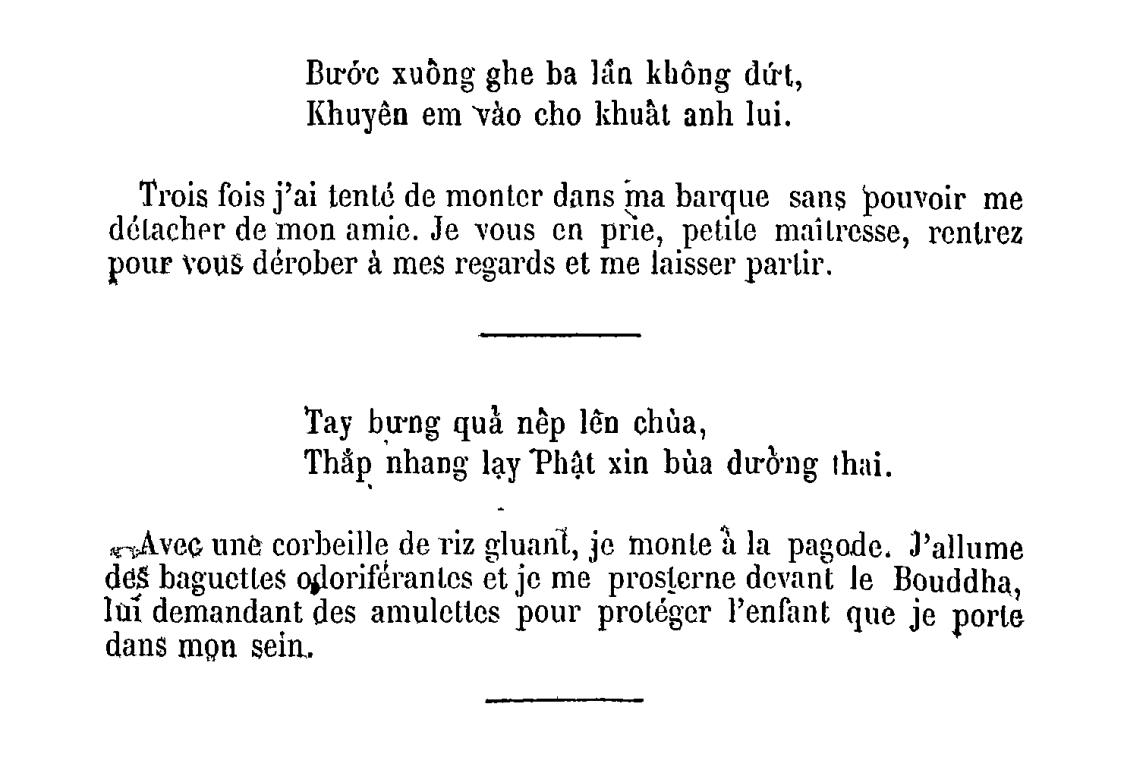
\includegraphics[width=1\linewidth]{img/1896.PNG}
    \caption{Chantes populaires et proverbes annamites} \footnote{\cite{cadao}}
    \label{fig:1896}
\end{figure}
Les chants populaires vietnamiens ont été traduits et présentés pour la première fois dans le Bulletin de la Société des Études Indochinoises en 1896 (voir figure \ref{fig:1896}). Avant l'apparition de l'écriture et encore aujourd'hui, les Vietnamiens ont une habitude culturelle de transmettre des connaissances de manière orale et de se souvenir de chants populaires (ca dao) et de tuc ngu (proverbes) pour communiquer des messages, des leçons de morale et des expériences agricoles dans la vie quotidienne. 
Comme dans de nombreux pays, la littérature orale et populaire précède souvent, voire toujours, la littérature écrite. Ces phrases, ces chansons et ces écrits sont transmis de bouche à oreille, de génération en génération, sans que l'on sache de nos jours qui en était l'auteur authentique. »\footnote{\cite{tinh}}
Dans un numéro du B.S.E.I de l'année 1963, un article décrit la science au Vietnam.

« Dans l'ancien Vietnam, la science expérimentale, telle que nous la concevons en Europe, n'a pour ainsi dire pas existé. Ce phénomène était d'ailleurs général en Asie, et la Chine, comme l'Inde, jusqu'au contact avec les Occidentaux, possédaient surtout une science empirique et des techniques traditionnelles. La culture chinoise, guère différente de la culture du Moyen-âge européen, accordait une place privilégiée et prépondérante à la littérature, à la philosophie et à la morale »\footnote{\cite{bsei}}

La transmission du savoir et de la culture dans les régions du Vietnam, du Laos et du Cambodge a une histoire profondément enracinée, débutant principalement par une tradition orale. L'éducation traditionnelle trouve son foyer dans les temples bouddhistes et confucianistes, particulièrement dans le nord du Vietnam. Les moines et les érudits de ces temples, vénérés en tant que sages respectés, se consacraient à l'étude des écrits en chinois, qui étaient la langue des textes classiques avant l'avènement du chu-nom et de la romanisation vietnamienne. Ces érudits, tout en étant des gardiens du savoir, étaient également des statues de moralité symbolique. Ils étaient étroitement liés à la communauté et à la population locale. Le tout premier établissement universitaire au Vietnam était le Temple de la Littérature, lui-même un temple confucianiste.

Au Vietnam, il existait également des enseignants privés qui dispensaient des cours particuliers, principalement destinés aux étudiants masculins, en vue de les préparer aux examens organisés par la cour royale. Ces examens visaient à conférer des titres pour occuper des postes gouvernementaux impériaux. Ces examens portaient principalement sur « Văn » (y compris la littérature, la philosophie, la morale), c'est pourquoi les intellectuels vietnamiens sont également désignés sous le terme de lettrés. Ces pratiques représentaient les manifestations majeures de la compétition intellectuelle dans la tradition confucéenne. Les influences de la culture chinoise, de l'astronomie et du calendrier lunaire étaient également omniprésentes et appliquées, en particulier dans le domaine de l'agriculture, notamment la culture du riz. 
Les régions montagneuses et les collines du Vietnam, couvrant une grande partie de son territoire, ont vu l'émergence de techniques sophistiquées de terrassement et de systèmes d'irrigation adaptés aux rizières.

La classe intellectuelle et l'élite au Vietnam étaient fortement influencées par la culture chinoise, maîtrisant les caractères chinois et adoptant les idées confucéennes. En plus de leurs rôles d'intellectuels, ils occupaient des postes de haute importance au sein du gouvernement en tant que mandarins, tout en nourrissant un fort patriotisme et un engagement envers leur patrie. Malgré près d'un millénaire de domination chinoise, le Vietnam a réussi à préserver sa culture et sa langue distinctives, même en face de nombreuses influences culturelles.

Le confucianisme, adopté en harmonie avec les croyances bouddhistes et les rituels ancestraux, a joué un rôle essentiel dans la construction de l'identité nationale et de la moralité au Vietnam. Le culte des ancêtres, le bouddhisme et le confucianisme ont renforcé les valeurs idéologiques et morales de la société vietnamienne. De plus, des croyances religieuses telles que le taoïsme et le caodaïsme, propres au peuple vietnamien, ont également émergé. La langue nationale a également joué un rôle essentiel dans la formation de l'identité nationale.

Au Laos et au Cambodge, deux pays majoritairement bouddhistes Theravāda, les moines occupent une place centrale dans l'enseignement, en particulier pour la langue principale, le khmer, et la médecine. Les monastères servent de centres éducatifs et religieux.

En ce qui concerne l'architecture et l'ingénierie, notamment les monuments d'Angkor au Cambodge, les palais et les pagodes, un niveau élevé de compréhension professionnelle et mathématique était requis. L'Indochine a connu un développement rapide de l'agriculture, en particulier de la culture du riz. Le climat tropical, caractérisé par des pluies abondantes, une chaleur constante et une humidité élevée, favorise une croissance rapide des plantes, bien que les risques climatiques soient également fréquents. Pour cette raison, les savoirs agricoles, fondés sur l'observation des étoiles et des cycles lunaires sont importants.

Les régions du Vietnam, du Laos et du Cambodge ont une histoire riche et complexe de transmission du savoir et de la culture, ancrée dans des traditions orales, des institutions religieuses, et des pratiques agricoles sophistiquées. Ces sociétés ont évolué au fil du temps, tout en préservant leur identité culturelle distincte malgré des influences extérieures importantes.

« La transformation culturelle commence par l'écriture,
Il en résulte qu'à partir du XIIIe siècle, parallèlement à la littérature orale, deux littératures écrites ont coexisté : la littérature sino-vietnamienne en chinois classique d'une part, la littérature en nom, c'est-à-dire en langue vietnamienne transcrite à l'aide de caractères chinois, d'autres part – cette dernière, composée en vers, étant reléguée au rôle de divertissement.»\footnote{\cite{tung}}

L'émergence du Chu-nom au début du Xe siècle représente une innovation notable au Vietnam, puisqu'il utilise le chinois comme un instrument de communication. Cette approche ingénieuse consiste à emprunter les caractères chinois pour exprimer les sons et les significations vietnamiens, tout en préservant une certaine autonomie par rapport au sens du mot d'origine.

On peut dire qu’après X siècles de domination, la société vietnamienne a accepté le concept de science chinoise sans grande évolution. Cependant, les influences du confucianisme, entendues ici comme les valeurs littéraires, philosophiques et éthiques promues, sont profondément ancrées dans les familles et les villages du Vietnam. L'apparition ultérieure de la science occidentale est considérée comme la deuxième fois rétablissant un nouveau concept avec des concepts scientifiques, visant la raison et l'exactitude. La domination française avec son appareil civilisationnel occidental n’était donc pas qu’une simple délocalisation géographique. Cela signifie également une profonde transformation idéologique.

« L'anomalie n'apparaît que sur la toile de fond fournie par le paradigme. Plus la décision et la portée du paradigme sont grandes, plus celui-ci se révèle un indicateur sensible pour signaler les anomalies et amener éventuellement un changement de paradigme.»\footnote{\cite{klun}}
L'anomalie dans le cas du Vietnam, cela peut être compris comme l'émergence d'un nouveau régime colonial, après la Chine, avec le droit d'imposer de nouveaux « paradigmes » à la société vietnamienne, même s'ils sont contraires à l'ancienne institution.


\section{L'histoire coloniale indochinoise}
L’histoire coloniale (ou l’histoire des empires colonial) est une champs de recherche souvent considérée comme « une histoire à marge », avec plusieurs concepts scientifiques possibles en contexte colonial, anti-colonial ou postcolonial… qui tournent autour le temps de colonisation, le territoire ou l’humain central qui sont concernés. Cette notion de l’histoire est pourtant cachée des domaines interdisciplinaires qui se croisent parmi plusieurs sciences humaines différentes : histoire, sociologie, anthropologie, géographie, politique… comme elle n’est loin de l’histoire d’une nation mais des empires coloniaux avec toute leur complexité. \footnote{\cites{Dulucq2003UneHE}}

Pour le cas de la France : 
« D’abord, de 1789 à l’adoption définitive du drapeau tricolore et du suffrage universel masculin, la France aurait fondé sa nation à travers ses Constitutions et ses processus internes de politisation.
Ensuite, la nation politique aurait fait sien l’héritage colonial ancien et s’est agrégé un empire, qu’elle n’a pas mêlé à la République. Autrement dit, rien d’essentiel dans la fondation de la nation ne se joue dans l’outre-mer colonial. La « Plus Grande France » n’est pas une République de citoyens et ce montage juridique commande une historiographie segmentée.»\footnote{\cites{Annales06}}

L’histoire de l’Indochine française ne fait pas exception, elle s’inscrit entièrement dans l’histoire des colonies françaises sous le drapeau tricolore avec toutes ses caractéristiques, pourtant, cette histoire désigne les « français » ne sont pas comme les « autres », les « français asiatiques » avec leurs bagages culturels différents, un climat tropical et ses histoires d’un autre continent que l’Europe.

Les relations entre le Vietnam en particulier et l'Indochine en général ont commencé avec des contacts religieux catholiques, au début des conflits entre les dynasties Trinh et Nguyen au XVIIe siècle. La Fondation de la Société des Missions étrangères a été fondée en 1647, ouvrant officiellement la voie aux activités des Jésuites dans le monde.

Parmi eux, Alexandre de Rhodes, après son arrivée au Vietnam, avec ses efforts en matière de langue, d'éducation et de mission, rédigea Le Dictionarium Anamiticum Lusitanum et Latinum, le premier dictionnaire à introduire la langue nationale, la romanisation de la langue nationale. connue sous le nom de transcriptions du vietnamien en caractères latins. Un alphabet vietnamien basé sur les lettres latines s’est progressivement formé. Ces idées ont permis aux Européens, en particulier aux missionnaires, de comprendre et d’apprendre le vietnamien à cette époque et ont contribué à façonner l’écriture du vietnamien moderne. Ainsi avec Alexandre de Rhodes « On peut considérer qu’entre la France et le Vietnam il est le premier « passeur de civilisations ».\footnote{\cite{phil}}

Au cours des deux siècles suivants, outre les échanges continus entre la France et le Vietnam à travers les lettres des missions et des députés européens, s'effectua également un commerce maritime avec l'échange de marchandises telles que la soie, les épices et la céramique. Cependant, ces activités ne sont pas encore considérées comme une relation clairement établie.

Participation militaire de Pigneau de Behaine -évêque d'Adran à la lutte de Nguyen Anh contre les Tay Son entame une relation diplomatique et politique entre les deux pays. À partir de ce moment, on peut parler d’une phase silencieuse de précolonisation. Puis, l'année 1825 fut le début des persécutions religieuses par l'empereur Minh Mang, cela prévient un "danger" hors orient qui se présente déjà dans la société. 

\begin{figure}[H]
    \centering
    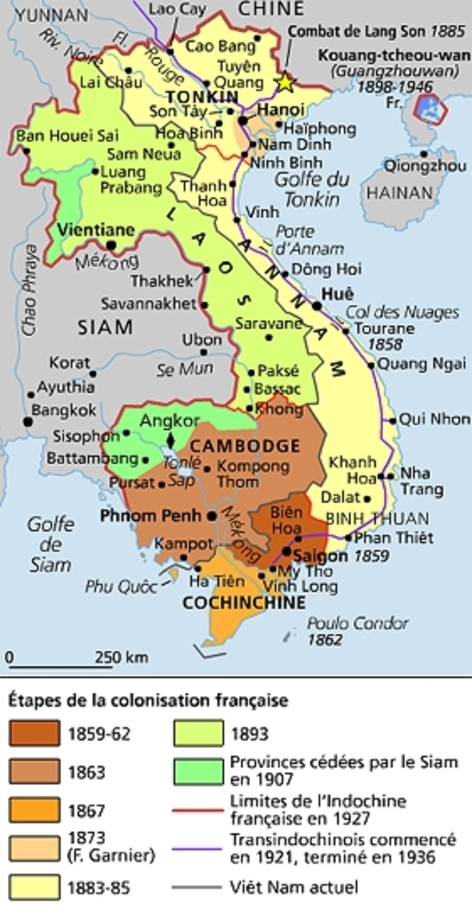
\includegraphics[width=0.5\linewidth]{img/1.1.union indochinoise.jpg}
    \caption{L'Union Indochinoise et ses étapes de la colonisation française}
    \label{fig:enter-label}
\end{figure}

« À partir du milieu du XIXe siècle, le royaume Dai Nam des Nguyen passe progressivement sous l’autorité française : après l’attaque du port de Tourane (actuellement Đa Nang) en 1858, Saigon est prise en 1859, le sud du pays devient une colonie française sous l’appellation de Cochinchine à partir de 1862 et le reste du pays, divisé en Tonkin et Annam, entre définitivement en 1884 dans l’Empire sous le régime du protectorat. La langue française étant la langue de l’administration coloniale, on forme des interprètes et autres auxiliaires indispensables à la marche des services. Il est logique de penser que les idées des Lumières ont dû s’introduire au Vietnam directement dans les fourgons du français. »\footnote{\cite{colon}}

L'un des principaux objectifs de cette colonisation était la Mission Civilisatrice. L'application de cette mission, quel que soit le territoire colonial, s'avérait complexe. Dans le cas spécifique du Vietnam et de l'Indochine dans son ensemble, cette mission revêtait une importance primordiale, symbolisant la transition des concepts scientifiques de l'orient vers l'occident.

« Plutôt « mission », d’amener ces civilisations inférieures au niveau de la civilisation française »
Des dichotomies telles que « Noir » et « Blanc », « sauvage » ou « barbare » et « civilisé », apparaissent alors comme autant de moyens mis en œuvre par le colonisateur pour justifier la domination des colonisés» \footnote{\cite{afri}}

Au commencement, au sein des colonies, des institutions intellectuelles et scientifiques coexistaient avec l'administration coloniale. Leur mission première était d'acquérir une compréhension approfondie des territoires colonisés, tout en contribuant aux buts plus larges de la colonisation. Toutefois, au fil du temps, des institutions universitaires autonomes ont émergé, poursuivant leurs propres objectifs de recherche indépendants. Les sociétés savantes constituent également une illustration de cette évolution. 
Cependant, \textit{que représente précisément la Société des études indochinoises ?}


%%%%%%Dans lequel la science ne fait pas partie importante, c'est pour ça que valoriser. Au XXe siècle, l'imprimerie s'est d'abord développée au Vietnam, Organisations et sociétés scientifiques savantes en générale


\section{Une première notion de la société savante}

La première société savante, qui reste la plus prestigieuse de ce statut est Académie des Inscriptions et Belles-Lettres - depuis 1652. Selon la définition de écrit par Régis Bertrand (Fédération historique de Florence) écrit dans le 1e Bulletin de liaision des sociétés savantes comme « une société qui produit et diffuse de la recherche, un groupe organisé dans un champ disciplinaire donné dont les adhérents ont pour objectifs de rendre compte de leurs travaux, d'améliorer la connaissance dans leurs domaines, d'assurer la formation et la recherche, de diffuser les résultats de leurs activités, de soutenir et de promouvoir leur discipline.»{\footnote{\cite{bum}}}

« la société de savoir pratique une attitude simplement cumulative des connaissances. Sonsouci n'est pas de mieux comprendre le monde qui l'entoure mais simplement d'engranger davantage de noms propres, de dates, de faits, et de descriptions. Jean Cluzel, secrétaire de l'Académie des sciences morales et politiques, évoque le rôle civilisateur de ces sociétés « dépositaires des anciennes traditions locales » {\footnote{\cite{alkd}}}

Il y a diverses définitions, cependant, les éléments généraux que nous retenons sont qu'une société savante se définit comme une organisation scientifique rassemblant des individus issus de diverses disciplines, tous animés par la volonté de développer la connaissance dans un domaine spécifique d'étude. L'adhésion à ces sociétés repose sur la volonté des membres de participer activement, cette participation étant soumise à l'approbation de leurs pairs. En plus de promouvoir la compréhension de l'objet de recherche, une société savante s'apparente à un institut intellectuel et comporte des éléments fondamentaux, notamment un conseil d'administration composé de présidents et de membres de l'association, un porte-parole scientifique, ainsi que diverses activités, telles que des séminaires et des cours en collaboration avec d'autres organisations scientifiques, généralement d'autres sociétés savantes.

Il est important de noter que les sociétés savantes fonctionnent selon un modèle horizontal, ce qui signifie qu'elles jouissent d'une certaine indépendance et ne sont pas directement subordonnées à une autorité académique supérieure. Elles établissent leurs propres normes et critères, et leur principale source de motivation réside dans la passion pour la recherche. Les considérations liées à la carrière et aux postes académiques ne sont pas prioritaires, la curiosité intellectuelle et la volonté d'explorer l'inconnu étant au premier plan. Dans le contexte des environnements coloniaux, caractérisés par des facteurs sociaux, géographiques et politiques inédits, de nouvelles disciplines scientifiques ont émergé, incitant les chercheurs à se tourner vers l'autoformation à partir des ressources scientifiques disponibles. Parallèlement, les sociétés savantes étaient interconnectées horizontalement, partageant une motivation commune visant à promouvoir une compréhension scientifique nouvelle.

Au sein de ces sociétés, une personne pouvait être membre de multiples associations, favorisant ainsi la diversification de la recherche et l'émergence d'approches interdisciplinaires au sein d'une même étude. Ces organisations soutiennent la recherche grâce à des infrastructures telles que des bibliothèques, des musées et des activités de recherche sociale, tout en favorisant la création d'un réseau social scientifique entre les chercheurs. L'objectif était de favoriser les échanges, la progression collective et d'apporter des éléments contribuant à une vision globale de l'objet de recherche, ce qui est illustré ici par le cas de la Société des Études Indochinoises (S.E.I) focalisée sur l'Indochine.

Un représentant du ministère de l’Éducation nationale a défini la société savante comme « un tissu associatif vivant » et « un des canaux de relations entre la recherche savante et la société civile ». \footnote{\cite{bbu}}

En effet, une société savante ne se limite pas uniquement aux activités de recherche scientifique internes, mais elle s'étend également vers l'extérieur en proposant diverses activités sociales. Cela inclut la tenue de séminaires, l'organisation d'expositions, ainsi que l'établissement de musées et de bibliothèques accessibles au public, favorisant ainsi la diffusion de la recherche scientifique auprès de la société en général. En résumé, une société savante entretient une étroite relation avec la société dans son ensemble.

« Tous ces courants donnent différentes catégories d’historiographie coloniale. On peut en distinguer grosso modo trois types. La première est constituée d’écrits de non-spécialistes, militaires et "coloniaux", travaux qui sont généralement des œuvres de commande? La seconde provient des travaux de propagandistes liés aux intérêts politiques et économiques de la colonisation, rédigeant et diffusant un savoir destiné à développer la fibre coloniale. Dans cette catégorie hybride, on trouve des auteurs appartenant au premier genre, mais aussi des savants, mobilisés pour la cause et capables de synthétiser une production hétéroclite. L'exemple le plus emblématique en est l'ouvrage paru en 1886 sous la direction d'Alfred Rambaud, professeur d’histoire à la Sorbonne: La France coloniale, Histoire, Géographie, Commerce”; après la préface de l'universitaire, les différents chapitres sont essentiellement confiés à des administrateurs et à des explorateurs. La même année voit la sortie d’un best-seller, Les Colonies françaises, rédigé sous les auspices d’un autre universitaire » .\footnote{\cites{marge05}}

Les sociétés savantes françaises ne se cantonnent pas uniquement à la France métropolitaine, elles élargissent leur champ d'action là où la science peut progresser et où de nombreuses découvertes restent à faire. L'exemple des sociétés savantes coloniales représente une forme de diffusion du savoir scientifique à l'échelle mondiale.

« Le troisième type d'histoire coloniale — que l’on pourrait qualifier de savante - se développe dans un cadre universitaire. S’appuyant sur le socle de publications produites par les catégories précédentes, mais surtout sur les sources passées au crible de la critique méthodique, ceux qui l’écrivent sont le pur produit du nouvel enseignement délivré à la Sorbonne. Rien, ni dans la méthode ni dans l’esprit général du travail, ne les distingue des autres travaux d'histoire. Leurs thèses sont rédigées selon les critères de rigueur scientifique de l’époque et ceux qui peinent à les satisfaire sont le plus souvent écartés de la carrière universitaire......Dulucq, Sophie, and Colette Zytnicki. » \footnote{\cites{marge05}}

La présence de ces organismes dans les colonies suscite également des interrogations quant à l'objectivité de leurs recherches. Dans cette étude, nous partons du principe que même si certains aspects de l'organisation des sociétés savantes sont étroitement liés à la politique, les études menées peuvent néanmoins être sujettes à des biais. Dans le cas de la Société des Études Indochinoises (S.E.I), les méthodes des humanités numériques seront utilisées en partie pour aborder cette question. 


\section{Société des études indochinoises}
« La crise ne fut, d’ailleurs, que passagères ; et quelques jours après la dissolution du comité ses anciens membres, réunis en séance extraordinaire, adoptaitent en principe sa reconstitution en une société libre appelée Société des Études Indo-chinoises »\footnote{\cite{soci}}

En quoi consiste exactement une société savante « libre » ? Comme l'indiquait le président George Dürrwell de la Société des Études Indochinoises dans son rapport adressé à Monsieur le Gouverneur général de l'Indochine le 30 septembre 1903, comme cité précédemment.

Après s'être « affranchie » du comité agricole et industriel de la Cochinchine, la nouvelle société, dotée de toutes les ressources précédentes mais arborant une nouvelle forme, est née. B.S.E.I a été fondée le 23 janvier 1883, immédiatement après la "suppression et la dissolution" du Comité agricole et industriel de la Cochinchine (1965-1883).

Si juste avant le Comité « fut placé sous la présidence du capital de frégate Fauque », « fut constituée avec des officiers de terre et de mer, soldats improvisés colons de la première heure »\footnote{\cite{a}} avec des missions bien définies dans le développement agricole de la colonie, l'organisation d'expositions, et bien sûr « dont les travaux insérés dans les bulletins du Comité prouvent qu’avec de la bonne volonté et de la persévérance, le Français est à la hauteur de toutes les situations » \footnote{\cite{a}}, et au cours de ces 18 années de développement, le Comité, dont il était l'un des «premiers ouvriers de la conquête dont les noms sont inscrits de droit au Livre d’Or de la Cochinchine » \footnote{\cite{soci}}. 

À ses débuts, le Comité agricole et industriel était un organe formel, peuplé en grande partie d'officiers de l'occupation française en Indochine. Son objectif initial était de superviser les expositions annuelles des produits locaux. La société fonctionnait selon des statuts rigides, avec des membres nommés par le gouverneur colonial.

Et au « 1er Octobre, le Comité comptait 107 membres et il était en rapport avec 17 sociétés savantes françaises ou étrangères. » \footnote{\cite{a}} . Cette phase prend fin, marquant ainsi la clôture de la première période historique et l'émergence d'un nouveau rôle en tant que revue continue du Bulletin de la Société des Études Indochinoises (B.S.E.I).

Toutefois, l'évolution politique et sociale de l'Indochine a provoqué une évolution majeure au sein de la S.E.I. En 1883, l'adoption de nouveaux statuts a marqué un tournant vers une structure plus démocratique. Désormais, les membres étaient cooptés plutôt que nommés, et la société bénéficiait d'une plus grande autonomie par rapport à l'administration coloniale à l'époque. 

Au fil du temps, la S.E.I. a élargi sa sphère d'intérêt pour englober une palette diversifiée de domaines, dans le statut de la société publiée année 1906 : 

« La S.E.I., continuant l'œuvre du Comité agricole et industriel, a pour objet l'étude de toutes les questions relatives tant à l'archéologie, aux arts, à l'ethnographie, et folklore, à la géograpbie, à l'histoire, à la philosophie, et aux religions, qu'à l'agri-culture, au commerce, à l'industrie et aux sciences de l'Indochine; elle s'intéresse aussi au rôle imparti à l'Indochine dans l'Extrême-Orient; elle conserve et transmet les monuments, archives et documents de toute nature, qu'européens qu'indigènes. »\footnote{\cite{bseik}}

La société a publié un Bulletin de ses travaux, entretenu des collections, participé à des expositions, commission et offert son soutien moral et intellectuel à diverses initiatives liées à ses domaines d'étude. Il conclut en notant que la société a publié un grand nombre d'articles au cours de ses 92 ans d'existence. Elle est constituée de plusieurs entités distinctes, notamment sa bibliothèque, sa scientifique et son musée.

Le Bureau de la société est composé d'un président, de deux vice-présidents, d'un secrétaire, d'un bibliothécaire, d'un trésorier et d'un conservateur de musée. Ces membres sont élus pour une durée d'un an et sont éligibles pour la réélection. Les élections pour le prochain Bureau ont lieu lors de l'Assemblée générale annuelle en décembre.

La société accueille un nombre illimité de membres, mais pour être admis, un candidat doit être parrainé par deux autres membres de l'association et doit obtenir les votes favorables de 2/3 des membres présents. Les membres peuvent également être révoqués de leur statut dans certaines circonstances, telles que leur démission volontaire, une absence prolongée ou s'ils sont exclus par les autres membres de l'association.

Il existe trois principales catégories de membres au sein de la S.E.I : les membres honoraires, qui sont désignés par le Bureau et qui peuvent être des étrangers, des fonctionnaires ou des individus ayant contribué de manière significative à la recherche sur l'Indochine ; les membres titulaires, qui résident en Indochine ; et les membres correspondants, qui résident à l'extérieur de la région.

Selon Martine François dans son article de \textit{Les sociétés savantes et l’histoire des voyages et des explorations} :
« Nous pouvons distinguer trois types de sociétés susceptibles d’avoir conservé des fonds intéressant les voyages, tout d’abord, celles créées spécialement pour étudier un pays, un continent, ce qui légitime la constitution de ces fonds."\footnote{\cite{ak}}
« Les sociétés consacrées à des pays ou à des continents Dès le milieu du XIXe siècle des sociétés savantes furent créées dans les territoires nouvellement colonisés comme la Société d’histoire et d’archéologie de Constantine, la Société historique algérienne, l’Académie d’Hippone, la Société des études indochinoises, l’Institut de Carthage, la Société des sciences, lettres et arts de la Réunion ou l’Académie malgache. Ces sociétés ont été les premières à étudier l’histoire et l’archéologie de ces pays nouvellement découverts. » \footnote{\cite{ak}}

En réalité, la Société des études indochinoises (S.E.I) est réputée pour être une société érudite dédiée à l'étude de pays ou de continents spécifiques. La Société des Études Indochinoises n'est pas la seule société savante coloniale française. On peut mentionner d'autres organisations de ce type, notamment aux colonies françaises : 

\begin{itemize}
    \item Société royale des Artes et des sciences de l’Ile Maurice
    \item Société d’agriculture d’Alger
    \item Société géographie et d’archéologie de la province d’Oran
    \item Société des sciences et art de la Réunion, ect.
\end{itemize}

En Indochine : 
\begin{itemize}
    \item Société médico-chirurgicale de l'Indochine \footnote{\cite{al}}
    \item Société médicale de Saigon – SAIGON\footnote{\cite{ab}}
    \item Société de géographie d'Hanoï (1921-)
    \item L'école française d'Extrême-orient
    \item Association des Amis du Vieux Huê
\end{itemize}

En 1933, lors de la célébration du cinquantième anniversaire de sa fondation, la Société des études indochinoises (S.E.I) avait déjà émis un total de 388 numéros de publication. Cela indique qu'en comparaison avec l'ensemble des journaux dont nous disposons des données pour notre corpus sera 1342 articles, la période qui est suivie n'a duré que 42 années. Toutefois, il est remarquable que leur productivité ait considérablement augmenté par la suite (1933-1975), atteignant finalement un total de 954 numéros de publications.

En 1893, la société a élargi ses horizons en introduisant le tourisme au sein de ses activités, sous l'impulsion de M. Commençait. Cependant, cette initiative a failli causer sa perte en 1925 lorsque le Bulletin a fusionné avec la Revue du Tourisme. Heureusement, la société a réussi à rebondir l'année suivante, en 1926.

Le logement en premier temps a toujours été un défi pour la société. En 1887, elle a été brusquement expulsée de ses locaux et a déménagé précipitamment, stockant sa bibliothèque, ses archives et ses meubles dans un compartiment de case malabare. Elle a ensuite loué un immeuble à colonel Rheinart pour 50 dollars par mois en 1887, puis a élu domicile à la société Philharmonique en 1891. En 1897, elle a emménagé au 16 rue Lagrandière, un immeuble appartenant à l'Évêché, où elle est restée pendant 20 ans. Enfin, elle a trouvé un emplacement stable au 12 Boulevard Norodom, dans un immeuble chrétien, pour 10 000 francs.\footnote{\cite{societe}}

L'un des moments forts de la société a été la contribution de M. Mercier Beauné en 1893, lorsqu'il a présenté des pierres préhistoriques gravées trouvées à Tay Ninh. En février 1897, un "air anthropologique" est né grâce à M. James, rédacteur en chef du Courrier de Saigon, qui a partagé des objets étranges parmi les membres, dont des armes, des colliers, des bijoux en os, en pierre et en cuivre, ainsi que des fragments de squelettes. Il a promis de céder une partie de sa collection à la société. Le général de Beylié a également contribué en fournissant d'importants moulages de vieilles pierres artistiques d'Angkor au musée\footnote{\cite{societe}}. 

Ces pionniers experts ont joué un rôle fondamental en traçant les premières lignes directrices de la recherche au sein de la Société des Études Indochinoises, marquant ainsi une transition significative dans leurs domains de recherche.

À une époque où l'Indochine était encore largement associée à l'agriculture et à l'exploitation des ressources naturelles, ces experts ont apporté une perspective nouvelle en se tournant vers l'archéologie et la préhistoire. Leur vision audacieuse a ouvert de nouvelles avenues pour la compréhension de l'histoire ancienne de la région, jetant ainsi les bases de la recherche archéologique et préhistorique qui allait suivre.

Le fonctionnement de la société a été un défi constant en raison de ses préoccupations scientifiques et philosophiques, conjuguées à des besoins matériels : 

« Les plus hautes préoccupations scientifiques et philosophiques y ont fait bon ménage avec des soucis très matériels: le local, le musée, les cotisations, les subventions, l'argent, pour tout dire en un mot, nécessaire non pas à rémunérer des travailleurs tous bénévoles, mais à payer le loyer, le personnel, l'éclairage, l'imprimeur, achats de livres, les abonnements aux revues, les timbres-poste et le papier de la correspondance parfois volumineuse qu'on échange avec l'Administration, avec les sociétés savantes d'outremer, avec les membres de la métropole... »{\footnote{\cite{societe}}}

Le 2 septembre 1945, à la place Ba Dinh de Hanoï, Ho Chi Minh proclama la création de la République démocratique et indépendante du Vietnam. La guerre de résistance commençait dans le Sud, également connue sous le nom de Nam Bô kháng chiên, fut un conflit armé qui a eu lieu après la Seconde Guerre mondiale. Il impliqua les Britanniques, les Indiens, une force opérationnelle française ainsi que les troupes japonaises du Groupe d'armées expéditionnaire japonais du Sud, qui se sont trouvés en opposition avec le mouvement vietnamien communiste, le Viêt Minh, dans le but de déterminer le contrôle du pays. 
Pour la toute première fois, notre société s'est retrouvée confrontée à des événements majeurs susceptibles de mettre en péril son existence. En effet, c'est la première fois que, en ouvrant les premières pages du Bulletin, nous avons été accueillis par un avertissement évoquant la situation politique actuelle. Dans le rapport moral du président de l'organisation, nous avons également constaté une préparation résolue à affronter d'éventuelles dérives. 

« L’année qui vient d’achever a été marqué par la volonté persistante de votre Comité de maintenir l’activité de la Société des études indochinoises dans la voie qu’elle s’est tracée dès le début de la guerre qui consiste à poursuivre sans défaillance l’œuvre entreprise il y a plus de soixante ans. »\footnote{\cite{moral1}}
Et aussi : 
« Quelle que soit l’incertitude du lendemain, une tache immense est offerte aux hommes de bonne volonté. Même si notre bulletin devait renoncer à paraitre, notre effort n’en serait pas ralenti et nous ne cesserions de susciter des recherches et d’accueillir, pour une résurrection très proche, le fruit de ces travaux »\footnote{\cite{moral1}}

Deux années se sont écoulées, mais la situation n'a montré aucune amélioration. En 1947, le président M. Berland a présenté un autre Rapport moral, marquant ainsi une nouvelle étape dans l'évolution de notre société. Cette fois-ci, des changements significatifs ont été apportés à notre statut, principalement en ce qui concerne les cotisations des membres. De plus, une recommandation audacieuse a été formulée : l'introduction de deux nouveaux titres inédits, celui de « membre bienfaiteur » pour ceux faisant un don de 200 dollars, et celui de « membre à vie" pour ceux qui contribuent à hauteur de 500 dollars en faveur de la société. 
« Au 9 Mars 1945, le nombre de nos sociétaires s’élevait à 507. Au 30 juin 1946, nous nous retrouvions 150. Cette chute verticale était imputable, pour une large part, aux rapatriements massifs et aux bouleversements introduits dans la vie de chacun »\footnote{\cite{moral}}
et aussi plus précisément dans l'article du projet de modification :
« Le comité arrête le détail des modifications aux statuts à soumettre à l’Assemblé Générale du 19 janvier, en ce qui concerne notamment le nouveau montant des cotisations, ainsi que l’adaptation du libellé de divers articles, relatifs à l’organisation nouvelle de l’Indochine. »\footnote{\cite{change}}


En ce qui concerne la présidence de la société, elle a été incarnée par des figures notables, dont :

\begin{itemize}
    \item \textbf{D. Mougeot (1883-1904)}, qui a été à la tête de la société pendant une période cruciale de son développement.
    \item \textbf{M. Dejean de la Bâtie (1904-1906)}, qui a poursuivi le travail de son prédécesseur.
    \item \textbf{M. Tanan et M. Durrwell}, qui ont partagé la présidence pendant une impressionnante période de 14 ans, marquée par des réalisations significatives.
    \item R\textbf{aphael Barquisseau (1933-)}, qui a apporté sa contribution à la société dans une période d'importants changements historiques.
   \textbf{ H. Berland (-1949)} qui a soutenu la société la période marquée par le changement de statut de la société
    \item \textbf{MM. Gayet Georges (1949-1950)} et Doan Quang Tuan (1950-1952), qui ont dirigé la société dans une période charnière.
    \item Enfin, le dernier président de la société, \textbf{M. Joseph Boquet (1952-1975)}, a exercé ses fonctions avec dévouement pendant 23 ans, marquant ainsi une ère importante de l'histoire de la société. Il a été épaulé par le vice-président Truong Vinh Tong.
\end{itemize}

Ces présidents, chacun à leur manière, ont contribué à l'épanouissement et à la renommée de la Société des Études Indochinoises, faisant d'elle une organisation emblématique de l'étude et de la préservation du patrimoine indochinois.


\subsection{\textbf{Activités de la société
}
}
La société des études indochinoises a joué un rôle essentiel dans un éventail diversifié d'activités et d'événements marquants au fil de son histoire, en Indochine et à l'international. Parmi les moments clés de son engagement, on peut citer :

\begin{itemize}
    \item Exposition de 1900 et Exposition coloniale de 1931 : La société a pris part à ces expositions prestigieuses, contribuant ainsi à mettre en lumière la richesse culturelle de l'Indochine.
    \item Communication au Congrès des Sociétés Savantes (1891) : Une communication significative sur les ressources naturelles indochinoises a été présentée par J. Schroeder, illustrant l'expertise de la société dans ce domaine.
    \item Congrès International d'Histoire des Relations Culturelles entre l'Occident et l'Orient à Tokyo (1957) : Un événement d'envergure internationale auquel la société a participé activement, favorisant ainsi les échanges culturels.
    \item Exposition d'Arts et d'Archéologie du Vietnam à Washington (1960) : La société a contribué à cette exposition majeure qui a permis de partager la richesse artistique et archéologique du Vietnam.
    \item Exposition d'Art Français au Japon à Tokyo (1961) : Une autre manifestation témoignant de l'influence culturelle et de la coopération internationale soutenue par la société.
    \item Conférence Régionale Asiatique sur l'Éducation des Adultes (1951) : La société a activement participé à cette conférence d'importance régionale, mettant en avant son engagement dans des domaines divers, dont l'éducation.
\end{itemize}

\subsection{{Mussée Blanchard de la brosse
}}

Un des éléments importants dans l'identité de la société savante indochinoise est également le rôle central joué par la S.E.I. dans la création du Musée archéologique et artistique de Saigon (Musée Blanchard de la brosse, le nom d'un diplomate et gouverneur colonial français). Initialement, l'idée de créer un musée n'était pas à l'ordre du jour, mais au fil du temps, la société a progressivement investi dans ce projet, contribuant à rassembler des objets et des spécimens d'origine indochinoise pour ce qui allait devenir une institution culturelle significative.

Depuis l'année 1897 a été témoin d'un moment décisif lorsque Ludovic Jammes, membre éminent de la société, a émis la proposition audacieuse d'une expédition dans les environs de Pursat, au Cambodge. Son objectif : collecter des objets préhistoriques. Le succès de cette expédition a rapidement incité la société à créer une commission dédiée à l'étude et à la mise en place d'un musée ouvert au grand public. La Société des Études Indochinoises a dû surmonter de nombreux défis au fil de son histoire, des difficultés financières et des conséquences de la Première Guerre mondiale aux promesses non tenues pour la construction d'un musée du gouvernement, et ce, jusqu'au 14 août 1929, marquant une date mémorable, le musée archéologique et artistique de Saigon a été officiellement inauguré lors d'une cérémonie imposante. Cela a dû être une décision importante, car la fondation a dépensé jusqu'à 45 000 piastres pour acheter la collection de M. Holbé comme plate-forme d'exposition pour le musée, sachant que la cotisation de l'association n'était que d'1 piastre par mois et que l'association ne disposait que d'environ 200 personnes. Cette décision fit alors grand bruit dans la presse indochinoise à propos d'un musée Blanchard de la brosse nouvellement né.  

« Au temps où il arrivait à Saïgon, mourait dans cette ville un ancien pharmacien de la marine, le docteur Holbé qui, au cours d'une longue carrière passée toute entière dans nos parages, avait réuni avec infiniment de science, d'admirables pièces d'art chinois, japonais, coréen, thibétain, khmer, siamois, javanais et indou. »\footnote{\cite{collection}}

Peu de temps après, il a ouvert ses portes au grand public, offrant ainsi à tous un accès aux richesses culturelles et historiques de l'Indochine :
« M. Bouchot, conservateur du musée Blanchard de
la Brosse, rend compte que le nombre des visiteurs du musée pour le mois de février 1929 s’est élevé à 10.458 contre 10 883 en janvier. » Dont 3932 Européens et 6526 indigènes.\footnote{\cite{bouchot}}

La société a continué à une participation actif dans la gestion du musée, contribuant à son développement et à l'enrichissement de ses collections. Les présidents de la société ont joué un rôle essentiel dans cette entreprise, en mobilisant des ressources et en garantissant l'engagement continu de la société envers le musée. Un personnage important est Jean Bouchot(1929-1932) comme directeur et Louis Marius Malleret les conservateurs du musée pendant la période 1935-1949. Pourtant, du 1956 à 1979, par rapport au contexte historique le musée devient musée national du Viêt Nam à Saïgon.

Lorsqu'il s'agit d'évoquer le succès et la reconnaissance de la société au sein de la communauté scientifique, cela ne peut tout simplement citer le message de félicitation de l’École français d’Extrême-Orient de Louis Malleret : 
« La société des études Indochinoises héritière de la tradition léguée par l’ancien Comité agricole et industriel de la Cochinchine, l’avait précédé depuis 1883 dans la voie de travaux de recherches. Des officiers de marine et des érudits vietnamiens s’étaient associés très tôt pour accomplir un premier inventaire de connaissance et susciter un mouvement de découvertes dans le domaine de l’exploration géographique, des investigations archéologiques et des études philologiques. »\footnote{\cite{feli}}
et aussi
 « la société a connu trois guerres et s’est invariablement remise à la tache avec une nouvelle ardeur. »
« Depuis les temps ont passé, les générations se succèdent et les recherches scientifiques sont devenues plus pénétrantes et plus sûres de leurs méthodes et de leurs résultats. »\footnote{\cite{feli}}

Dans la dernière revue publiée en 1975, la société elle-même a également consolidé sa position dans le domaine des études indochinoises, comme en témoigne le comité de rédaction écrivait :
« Doyenne des sociétés savantes en Indochine. Créatrice du musée Blanchard de Saïgon, qu'elle administrait. La société d'études indochinoises, poursuit l'œuvre du Comité agricole et industriel créé en 1865. Elle compte dès 1883, 300 membres actifs européens et indochinois. Elle est en relation avec 38 sociétés savantes et universités françaises. »\footnote{\cite{fin}}
Ceci est également noté dans la page de définition de l'organisation pour S.E.I dans le site web de la Comité des travaux historiques et scientifiques.

\textbf{La bibliothèque de la société des études indochinoises
}
La Bibliothèque de la Société des études indochinoises occupe une place de premier plan dans le paysage intellectuel de l'Indochine. Depuis ses débuts, elle a été le réceptacle d'une multitude de dons de livres, chacun d'une valeur inestimable et provenant de sources diverses. Les collections de la bibliothèque sont riches et variées, reflétant la diversité des intérêts et des domaines de recherche de ses membres.

L'évolution de la Bibliothèque de la Société des Études Indochinoises est aussi un aspect à remarquer. La bibliothèque a été constituée par des dons de provenance variée, ce qui a donné à sa collection un caractère hétérogène. Elle s'est d'abord concentrée sur des domaines tels que l'agriculture tropicale, la zootechnie, les produits industriels et les sciences naturelles. Avec le temps, la bibliothèque s'est élargie pour englober des domaines d'études sur l'Indochine et l'Extrême-Orient.

L'héritage de la bibliothèque remonte aux premiers catalogues du Comité agricole et industriel, qui comprenaient des sections consacrées à l'agriculture tropicale. Au fil du temps, la bibliothèque s'est élargie pour englober des sections dédiées aux Beaux-Arts, à l'archéologie, à l'histoire, à la physique et aux sciences naturelles. Les collections de périodiques et d'ouvrages rares ont également trouvé leur place au sein de ses rayons.

La diversité culturelle de l'Indochine se reflète également dans les collections de la bibliothèque, qui abritent plusieurs fonds locaux, notamment chinois, khmer, laotien et siamois. Les estampes, les photographies et les manuscrits des membres de la société, tels que A. Adhémard Leclère, Silvestre, Charles Lemire, ajoutent une dimension précieuse à ces collections.

Au cours de son histoire, à notre connaissance, la bibliothèque a entrepris plusieurs réorganisations en 1927, 1930 et 1933, afin de mieux répondre aux besoins de ses membres et de garantir un accès optimal à ses précieuses ressources. Elle a également procédé à des achats urgents en réponse aux demandes spécifiques de ses membres, démontrant ainsi son engagement envers la recherche et la diffusion des connaissances.

« Mais, quoi qu'il en soit de ses défauts, elle n'en est pas moins l’un des centres de documentations les plus précieux que l'on possède en Indochine, sur les questions qui intéressent ce pays et l'Extrême-Orient La Bibliothèque de la Société des Etudes Indochinoises pourrait, dans une modeste mesure, jouer en Cochinchine, le rôle que détient au Tonkin la Bibliothèque de l'École française d’Extrême-Orient. Il lui appartient, en effet, de spécialiser son objet dans la réunion de tous les ouvrages qui se rapportent à l'Indochine et aux pays voisins. » \footnote{\cite{bilo}}. Parmi les ouvrages importants qui composent ses collections, on peut citer des œuvres historiques et scientifiques telles que :

\textit{Le Catéchisme en latin et en quôc ngu de P. Alexandre de Rhodes} (1651), \textit{Les Divers Voyages et Missions du P. Alexandre de Rhodes en la Chine et autres Royaumes de l'Orient} (1654), \textit{Le Recueil de plusieurs Relations et traités singuliers et curieux de J. B. Tavernier} (1679), \textit{La Relation des Missions et des Voyages des Évêques vicaires apostoliques ès années 1673, 1673, 1674 et 1675} (1680), \textit{Le Journal du Voyage de Siam fait en 1685 et 1686 par l'abbé de Choisy} (1687), \textit{Le Nouveau Voyage autour du Monde de Le Gentil de la Barbinais} (1728), ect. aujourd'hui considérés comme des trésors inestimables.\footnote{\cite{bilo}}

En matière de préservation et de diffusion du savoir, la Bibliothèque de la Société des Études Indochinoises est à juste titre reconnue en tant qu'institution éminente, établissant ainsi une égalité remarquable avec la Bibliothèque de l'École française d'Extrême-Orient. Ensemble, ces deux institutions contribuent de manière significative à l'enrichissement du patrimoine intellectuel de l'Indochine et à la compréhension approfondie de la région et de ses multiples facettes.


%Les membres sont membre de plusieurs sociétés savantes différentes."

%Discours politique, eurocentrique, discours colonial
%Dans le status de la société, la première fois apparait
%\textit{"Toute discussion politique ou religieuse est interdite"
%Ce changement remarque

\section{Le Bulletin de la société des études indochinoises}

Parmi les revues scientifiques les plus influentes dans le contexte de la vie intellectuelle en Indochine au début du XXe siècle, en plus des publications de l'École française d'Extrême-Orient (EFEO), du Bulletin des amis du vieux Hué (BAVH), de la revue Indochina, et de Littérature et Histoire, il est incontournable de mentionner le Bulletin de la Société des Études Indochinoises (B.S.E.I). Cette revue a vu le jour pour la première fois le 23 janvier 1883, et dès son premier numéro, à l'article 25, on pouvait lire :

« Le Bulletin est ouvert à la publication de tous les travaux susceptibles de diffuser la connaissance des diverses parties de l’Indochine, de leur géographie, de leur population, ressources, besoin, langues, ect. Il contient, de plus, les décisions de l'autorité concernant son œuvre, les-rendus des séances, des extraits ou des résumés des travaux étrangers intéressant les comptes régions indochinoises et un bulletin bibliographique, analytique autant que possible. »

Le nom du Bulletin est en étroite corrélation avec l'association SEI, car son objectif premier est la diffusion des connaissances scientifiques liées à l'Indochine. De plus, il joue également le rôle d'organe de communication de l'association, favorisant ainsi les échanges avec d'autres sociétés savantes en France et à l'international. Au cours de ses 92 années d'existence, la revue s'est engagée à évoluer bien au-delà de ses débuts modestes.

Dans un premier temps, le comité de rédaction du journal a envisagé la création d'un magazine mensuel de seulement 16 pages par numéro. Cependant, cette idée a rapidement évolué vers la publication d'une revue de 50 pages tous les trois mois, ce qui a été jugé plus réaliste. Le premier numéro ne contenait que deux rapports, et les numéros suivants maintenaient une moyenne d'environ 50 pages, comprenant des comptes rendus de la société et des articles sur l'organisation de l'association. Entre 1886 et 1887, la revue ne produisait que deux numéros par an (au lieu des quatre prévus), mais ceux-ci comptaient environ 70 pages chacun.

À partir du dernier numéro de l'ancienne série en 1919, la revue a progressivement augmenté sa pagination pour atteindre environ 200 pages par numéro. Les numéros de la nouvelle série ont même dépassé les 500 pages (comme le numéro 4 en 1953). Cette évolution témoigne de la croissance des intérêts et de l'expérience des auteurs, ainsi que de l'émergence d'une équipe d'auteurs de plus en plus solide, tant en termes de qualité que de quantité.

Il est important de noter que le B.S.E.I ne fixe pas de limites strictes en ce qui concerne le nombre de pages par numéro. La longueur des numéros varie en fonction de la diversité des genres et des sujets abordés. L'Indochine demeure un terrain de découverte scientifique, une jeune colonie, offrant ainsi aux auteurs et intellectuels éloignés de la France l'opportunité d'explorer et de comprendre cette région. Ils y trouvent un champ intellectuel stimulant et sérieux, tout aussi captivant que celui de leur pays d'origine.

De nombreux auteurs vietnamiens ont été éduqués dans le système occidental et ont fréquenté les écoles françaises dès leur plus jeune âge. Bien qu'ils parlent vietnamien, leur esprit scientifique et leur pensée théorique sont aussi développés que ceux de leurs homologues européens. Ils ont adopté des approches rationnelles et se sont rapidement intégrés à la vie intellectuelle en émergence. La diversité des contenus est une caractéristique majeure de la revue, et les exemples mentionnés ci-dessus ne représentent qu'une infime partie de la richesse du contenu global du journal.

\textbf{Thèmes de la religion} : Le bouddhisme en général par D. Migot (1946), Quelle est la religion des Annamites ? par L. James (1895), La religion les montagnards du Haut-Donnai par J. Dourne (1949), Contribution à l'étude du Culte des génies tutélaires ou Neak Ta chez les Cambodgiens du Sud par A. Souyris Rolland (1951) .. 

\textbf{Éducation} : L’enseignement en Cochinchine par G. Taboulet (1942), De l’enseignement du français en Indochine par J. B de Saint Michel, Le français et le vietnamien dans l’enseignement au Vietnam par Doan Quan Tan (1954) de la chimie Etudes des minéraux lourds de quelques sables littoraux par Hoang Ngoc Can (1964)

\textbf{L'ethnologie} : Le peuple en Asie par Teilhard de Chardin (1955), Études anthropologiques par P. Huard (1947), Notes d'ethnographie Cochinchinoise par C. Richard (1927), etc. 

\textbf{Géographie} : Les origines de Hanoi par G. Azambre (1958), Les mobiliers préhistoriques de l'abri sous roche de Tam Pong (Haute Laos) par E. Saurin (1966) 
Folklore laotien : Xine-Xay, par Thao NHOUY (1934) 

\textbf{Littérature vietnamienne} : Chinh phu nam khuc (Femme de guerrier) par Doan Thi Diem traduction Huynh Khac Dung (1955)… 

\textbf{Médecine} : De la diffusion de médecine européenne en Cochinchine par Péralle (1895), L'art de guérir chez les Annamites par L. James (1896), Histoire de l'acupuncture chinoise par P. Huard et Wong (1957)... 

\textbf{Les langues} : Petit vocabulaire laotien par J. Taupin (1892), Essaie sur l'origine de la langue  Annamite par G. Janneau (1883) ou La forme politesse en Javanais moderne par C. Damais (1950) 

Aussi nombreux articles sur \textbf{l’archéologie}, \textbf{l’histoire moderne}, \textbf{l'agriculture}, \textbf{la botanique}, \textbf{l'industrie}, \textbf{l'art}, \textbf{l'architecture}..
La revue B.S.E.I. (Bulletin de la Société des Études Indochinoises) se présente comme un véritable guide de l'Indochine, offrant une palette thématique d'une richesse étonnante. Cependant, il est révélateur de noter que, en 1923, la revue a connu de nombreuses difficultés pour assurer sa publication régulière.

Ces obstacles étaient principalement d'ordre économique, ce qui a conduit à des interruptions dans la publication en 1920, 1921, 1922, 1924 et 1925. Cependant, il est important de noter que ces interruptions dans la publication n'ont pas interrompu les réunions mensuelles de l'association. Les procès-verbaux de ces réunions ont été intégralement réédités pour que les membres puissent toujours accéder à ces informations, avec des numéros spéciaux en 1923 et 1926. Cela peut s'expliquer par le fait que la plupart des lecteurs de la revue sont des membres inscrits, et la responsabilité de l'éditeur peut inclure la réédition d'informations sur la société.

La revue B.S.E.I. ne se limite pas à être uniquement une publication scientifique, il sert également de lieu de diffusion pour toutes les informations liées à la société. Il fonctionne en quelque sorte comme un canal d'informations sur la société savante et les travaux de recherche scientifique de ses membres. Selon les statuts de l'association en 1883, la revue était distribuée gratuitement aux membres, tandis qu'une cotisation était due par les membres titulaires et correspondants. Cette cotisation était fixée à deux piastres par mois, payables trimestriellement et à l'avance, mais elle était réduite à 1 piastre par mois lorsque le nombre de membres titulaires dépassait cent. Les membres honoraires n'avaient pas de cotisation à payer.

Au cours de ses 92 années de développement, B.S.E.I. a connu deux périodes distinctes : l'ancienne série de 1883 à 1920, intitulée "Bulletin de la Société des Études Indochinoises de Saigon", puis la nouvelle série de 1926 à 1975, sous le nom de "Bulletin de la Société des Études Indochinoises". Durant cette période, les numéros étaient regroupés par année, avec un système de classement basé sur les "Tombe", chaque année comptant quatre numéros correspondant à chaque saison. Au total, B.S.E.I. compte 135 numéros au total, mais ces numéros ne sont pas numérotés séquentiellement, mais plutôt par année.

L'origine de B.S.E.I. remonte à son prédécesseur, le Bulletin du Comité, qui était principalement administratif. En 1883, il a évolué pour devenir un véritable bulletin d'études scientifiques. Présenter la revue B.S.E.I. est une tâche complexe, car elle est peu connue dans les résultats de recherche classiques, mais elle est considérée par les experts scientifiques comme une revue scientifique précieuse en tant que porte-parole de la plus ancienne société savante d'Indochine, non pas en tant que successeur d'une autre revue savante, mais pour ses propres mérites. En 1896, pour la première fois, les statuts de la société ont énoncé :

\begin{figure}[H] %[!ht]
    \centering
    
\includegraphics[width=1\linewidth]{img/tout.PNG}
    \caption{Statut de la société en 1896}
    \label{fig:enter-label}
\end{figure}

Une simple phrase, isolée de l'article Ier de ce texte, suggère que la société savante a peut-être réussi à évoluer au-delà de sa forme initiale de comité placé sous le contrôle du gouvernement colonial. Cette observation invite à prendre position en dehors des contextes politiques et religieux.

Cela étant dit, il existe un paradoxe notable, car même dans la plupart des numéros de la société pendant cette période, la liste des membres inclut toujours des personnalités telles que M. Le Gouverneur Général de l'Indochine en tant que président d'honneur, aux côtés de M. Le Lieutenant-gouverneur et du Général commandant la brigade de Cochinchine, entre autres, en qualité de vice-présidents d'honneur. De nombreux membres de la société étaient des individus travaillant au sein du gouvernement colonial, des fonctionnaires intellectuels dont les carrières étaient étroitement liées à la situation politique de l'Indochine à l'époque.

Cependant, malgré leur rôle dans le gouvernement colonial, ces individus étaient animés par une curiosité intellectuelle et un engagement envers la science qui les poussaient à s'engager dans des débats non politiques et non religieux, mais centrés uniquement sur les questions de recherche liées à l'Indochine.

Le B.S.E.I a hérité de son prédécesseur initialement un axe sur la mission d'apprentissage agricole et industriel, a progressivement élargi son champ d'intérêt pour englober tous les domaines liés à l'Indochine, avec une orientation claire vers la diffusion du savoir. En 1883, les trois premiers numéros du journal étaient centrés sur des sujets tels que "les grains jaunes du riz", "les cultures expérimentales", "les comptes rendus sur les courants terrestres", etc. Cependant, au fil du temps, la revue a évolué et diversifié ses thématiques, comme nous le démontrerons dans les analyses quantitatives ultérieures.

En raison du fait que notre compréhension actuelle de cette revue est encore en cours de développement, il existe très peu de sources extérieures d'information sur le B.S.E.I, à l'exception de ses propres publications. Les auteurs des articles publiés dans le B.S.E.I sont à la fois français et vietnamiens, et ils collaborent pour enrichir les connaissances. Parmi les Français qui ont contribué de manière significative, on peut citer : \textbf{André Baudrit, Jean Bouchot, Pierre Brocheux, Arthur Chéon, Pierre Daudin, George Dürrwell, Maurice Durand, Louis Ricard, Louis Malleret, Geogrette Naudin ; Henri Marchal}… 

\textbf{Henri Marchal }: \textit{Le chanteur d'Angkor Wat} (1934), \textit{Le temple de Banteay Srei} (1936), \textit{Notes sur Birmanie} (1950), \textit{Les travaux de la conservation d'Angkor} (1953), \textit{Notes sur un théâtre à l'ombres à Siem Reap} (1958), L\textit{Le Naga dans l'art khmer} (1937)… 

\textbf{Pierre Daudin} avec \textit{Vue ensemble sur la sculpture et la modelage en Chine durant vingt siècles} (traduction en 1936), \textit{Note sur un cachet en ou découvert en Annam} (1936), \textit{Sigillographie sino-annamite}(1937), \textit{Deux mandarins militaires de Thieu- Tri : Le Sam et Trieu Tan} (1943), \textit{Un Japonais à la Cours des T'ang, Gouverneur et protectorat d'Annam }(1965)… 

 \textbf{George Dürrwell} avec \textit{Les colonies militaires dans la Basse-Cochinchine} (1998), L\textit{e jeu en Cochinchine} (1901), \textit{La famille annamite et les cultes des ancêtres} (1908), \textit{La commune annamite} (1905),\textit{ Une visite à Ong-Yem : Les champs d'essai et la colonie pénitentiaire} (1909)… 

\textbf{Arthur Chéon} a traduit \textit{Des langues monosyllabiques du Sud de l'Asie} (K. Himly) (1886), \textit{Histoire de La-to ; La vase qui parle} (1889) ou \textit{Notes sur l'origine des chants populaires annamites} (1989), \textit{Notes sur la chanson cambodgienne} (1890) 

\textbf{Maurice Durand} : \textit{L'avenir des études vietnamiens }(1953), \textit{Chants des pêcheurs de Truong-Dong} (culte de la baleine) (numéro 2, 1953), \textit{Quelques éléments sur l'univers moral des Vietnamiens} (1952), A\textit{lexandre de Rhodes} (1957), \textit{Les impressionnants en vietnamien} (1961), L\textit{a Science au Vietnam} (avec P.Huard)( 1963) 

Selon nos observations, au fil du temps, le nombre d'auteurs vietnamiens participant à la rédaction de journaux augmente, les noms typiques incluent des intellectuels célèbres : 
Nguyen The Anh est spécialisé dans la rédaction d'articles historiques. 

\textbf{Vuong Hong Sen} avec des articles sur la culture chinoise \textit{La pagode de l'Empereur}(1950),\textit{ Le Jade à Dakao} (1950), \textit{Les pot à envoûtement, ancêtres des flacons à parfum moderne} (1949) 

\textbf{Nghiem Toan} et \textbf{Louis Ricard}, co-traducteur de contes chinois, peuvent citer \textit{Histoire du Ou Pao An} (1958). Leurs traductions sont d'une grande qualité, au point qu'aujourd'hui \textit{Les trois royaumes} (publié sur B.S.E.I de 1960 à 1963), le premier des Quatre livres extraordinaires de la littérature classique chinoise, sa traduction est rééditée aux éditions Flammarion depuis 2009 jusqu'à aujourd'hui. 

\textbf{Tran Van Khe} introduit \textit{Mise au point de l'étude sur la musique sino-vietnamienne et les chants populaires du Viêt-Nam} (1959) ou \textit{Place de la musique dans les classes populaires au Vietnam} (1959) 

Les deux frères \textbf{Truong Vinh Ky} et \textbf{Truong Vinh Tong}, dont \textbf{Petrus Ky}, participèrent dès les premiers jours au Bulletin du Comité et poursuivirent leurs écrits au B.S.E.I avec des articles sur \textit{L'Ecriture en Annam} (1888) ; \textit{Chuyen doi xua : Contes d'autres fois : Le genre qui veut intimider son beau-père} ; \textit{Le renard et le tigre} traduits par \textbf{Truong Vinh Tong} (1932), ect.
Toutes ces histoires ont été traduites en français par Truong Vinh Tong, son jeune frère, et le texte est présenté de manière bilingue. Il est intéressant de noter que, à l'exception de Truong Vinh Ky, les autres auteurs sont tous apparus après 1950, ce qui témoigne clairement de l'émergence d'une nouvelle génération d'intellectuels vietnamiens participant à la rédaction de la revue.

Dans le numéro de 1967, quelque chose de remarquable s'est produit pour la première fois dans B.S.E.I : des titres d'articles et des annotations bilingues en vietnamien avec des accents complets ont fait leur apparition. Cette évolution linguistique montre une ouverture vers une audience vietnamienne plus large. Même dans le numéro de 1972, il y avait un article consacré à la poésie de Han Mac Tu qui s'étendait sur 108 pages. Ces exemples de contenu bilingue et la diversification des sujets démontrent la volonté de la revue de s'adapter aux besoins de son lectorat.

Les noms mentionnés dans le texte ne représentent que quelques-uns des nombreux auteurs ayant contribué à des milliers d'articles publiés dans B.S.E.I. Ces auteurs sont tous des chercheurs importants, voire célèbres, dans leurs domaines respectifs. Cependant, il est important de noter que les contributions au journal ne se limitent pas aux articles signés. Il existe également des articles non signés, dont l'origine reste parfois mystérieuse. Il peut s'agir d'articles collaboratifs dont le nom des contributeurs a été oublié ou d'articles rédigés collectivement par la rédaction.

En somme, les idées du journal restent ouvertes à une exploration plus approfondie, à la fois au sein de ce projet et au-delà. La richesse de son contenu, sa diversité linguistique et la variété des contributeurs en font un véritable trésor intellectuel à découvrir et à étudier davantage.


Les 14 sujets ci-dessus sont répartis de manière relativement précise en documents administratifs, mais le travail restant à accomplir est de continuer à classer les documents des autres types.

\textbf{Actes de la société} : (1926 -1975) peut être considéré comme la deuxième phase du parcours de développement de la revue, comprenant des résumés des activités de l'organisation savante. Incluant : réunions, activités d'associations, assemblées générales, conférences des souvenirs, séances du mois...
Ou publications des sociétés correspondantes

\textbf{Catalogue} (1886-1887) comprend des livres récemment acquis par la bibliothèque, des artefacts exposés au musée et des collections connexes. 

\textbf{Nécrologies} : Gratitude et annonce de membres importants récemment décédés

\textbf{Publication} (1886-1937) : Comprend des index des essais, mémoires, dictionnaires, livres, bulletins publiés, monographies de la société, vendus aux bibliothèques de Saigon et chez Paul Geuthner à Paris

\textbf{Procès-verbaux} (1883-1975) : procès-verbaux sommaires des assemblées ordinaires mensuelles de l'association

\textbf{Liste des membres et assemblées générales }: Liste des membres, comprenant généralement un président d'honneur, un vice-président, des membres honoraires et des membres correspondants, des membres titulaires

\textbf{Société correspondante} Les sociétés savantes ont des liens scientifiques de coopération avec l'association, principalement en France et à l'étranger

\textbf{Bibliographie :} Généralement, ce sont des critiques de livres, des recommandations et des revues de livres récemment publiés sur le thème de l'Indochine

\textbf{Rapport }: il existe de nombreux types de rapport sous forme d'articles, rapport financier, rapport moral, rapport du trésor pour l'année ect.

L'évolution du Bulletin se décompose en trois sections, y compris la partie du Bulletin du Comité agricole et industrie, pourtant dans cett recherche, nous nous concentrerons uniquement sur la recherche B.S.E.I dans les deux dernières phases en tant que revue scientifique multidisciplinaire et de la société des études indochinoise. 

\section{L'État de la recherche et méthode de travail}

Les trois phases du modèle de Basalla (1967) sont illustrées sur la figure \ref{fig:ball_model}. Dans la première phase, Basalla explique que la "périphérie coloniale", composée de sociétés ou nations considérées comme non scientifiques, servait uniquement de source de données passive pour le développement de la science moderne dans les pays européens. Pendant cette phase, des scientifiques qualifiés ainsi que des amateurs européens tels que les explorateurs, les voyageurs, les missionnaires, et d'autres, visitent les nouveaux territoires, étudiaient et collectaient des informations sur leur faune et leur flore, examinaient leurs caractéristiques physiques, puis rapportaient les résultats de leurs recherches. \footnote{\cite{ball}} 

Dans la deuxième phase, une participation accrue de scientifiques est observée, marquant l'avènement de l'ère de la "science coloniale". Cette période voit l'implication de scientifiques coloniaux locaux ainsi que d'autochtones acculturés dans les travaux scientifiques.

La troisième phase vise à établir une tradition scientifique nationale indépendante en suivant les normes occidentales. Les scientifiques formés pendant la deuxième phase luttent pour surmonter les obstacles philosophiques et religieux à la science dans leur pays en favorisant une diffusion plus large de la connaissance scientifique.

\begin{figure}[H] %[!ht]
    \centering
    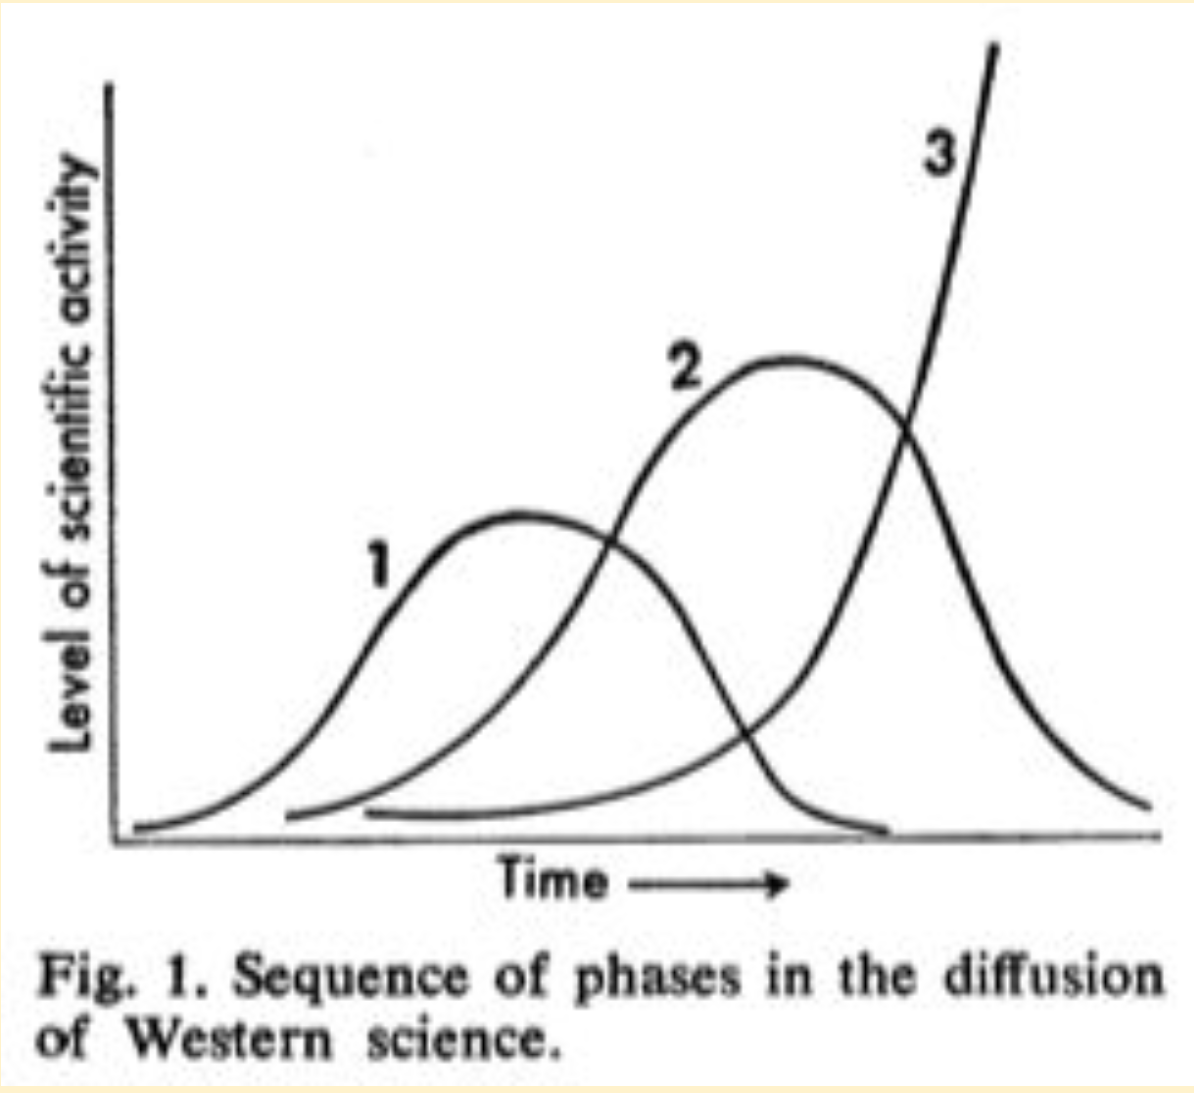
\includegraphics[width=0.5\linewidth]{img/ball's model.PNG}
    \caption[]{Modèle de Basalla \footnote{\cite{ball}} }
    \label{fig:ball_model}
\end{figure}

Nous soutenons l'idée que l'histoire de la science coloniale en Indochine, en général, suit également ce schéma, tout comme le processus de formation et de développement de la Société des Études Indochinoises (S.E.I) et de sa revue.

Si nous appliquons ce modèle au parcours du Bulletin de la Société des Études Indochinoises (B.S.E.I), nous pouvons estimer que la phase 1 correspond aux 18 premières années d'existence de son prédécesseur, le Bulletin du Comité Agricole et Industriel. La deuxième phase s'étend sur une période de 50 ans, de 1883 à 1933, tandis que la troisième phase commence à émerger de manière plus distincte à la fin des années 1960 et se prolonge jusqu'à la fin de la vie de la revue.

Notre étude se concentre sur une analyse temporelle des contenus de ce journal, dans le but d'identifier les principaux sujets scientifiques et de comprendre comment ils ont été présentés et développés au fil du temps. Cette analyse couvre la période allant de 1883 à 1975, année marquant la fin officielle de la publication du journal.

Pour mener à bien cette exploration, nous avons adopté une approche méthodologique basée sur les humanités numériques. Cette méthodologie implique l'utilisation d'outils et de techniques informatiques pour analyser et cartographier la distribution des contenus au sein du corpus, nous permettant ainsi de dégager des tendances et des évolutions dans les sujets scientifiques abordés.

En résumé, notre question de recherche se penche sur l'histoire du journal sur une période considérable, et nous abordons cette exploration avec une approche méthodologique moderne en nous appuyant sur les humanités numériques pour analyser et interpréter les données.

Premièrement, il convient de noter que grâce au développement de la technologie et à la prise de conscience de l'importance de préserver les sources documentaires anciennes, plusieurs projets ont récemment vu le jour pour numériser les sources de données indochinoises, notamment à ma connaissance, le projet \textbf{Vietnamica}\footnote{\cite{bibli}} et le projet \textbf{Patrimoines parrtagés}\footnote{\cite{partage}} entre Bibliothèque nationale de France et Bibliothèque nationale du Vietnam. Toutefois, ces sources restent largement sous-exploitées, notamment en ce qui concerne les recherches à grande échelle utilisant les humanités numériques. Lors de nos recherches de sources de référence pour cette étude, nous n'avons identifié qu'une étude récente menée par Emmanuelle Affidi sur le \textbf{Dong Duong Tap chi} (1913-1919)\footnote{\cite{duong}}, qui représente une tentative de diffusion du discours et de la science occidentale au Tonkin. Cette étude met en lumière les enjeux de l'interculturalité dans le contexte colonial entre savoir et pouvoir (1906-1936).

Cependant, il est important de souligner que ce nombre limité d'études demeure insuffisant pour exploiter pleinement le trésor de données disponible sur l'Indochine, qui comprend plus de 10.000 documents à la Bibliothèque nationale de France (BnF) et 540.000 pages de documents dans le cadre du projet Vietnamica.

Face à cette situation, et forts des compétences acquises au cours de notre spécialisation en humanités numériques, nous sommes convaincus que la recherche sur le Bulletin de la Société des Études Indochinoises (B.S.E.I) constitue le sujet le plus pertinent et approprié que nous puissions entreprendre. Ces recherches, en plus de la création d'un modèle d'alphabétisation multilingue, marquent les premières étapes d'une enquête plus approfondie sur l'histoire coloniale de l'Indochine et les relations entre le Vietnam et la France sur près d'un siècle d'exposition.

Un exemple qui nous a inspirés à entreprendre cette recherche est le projet de numérisation et de publication de l'ensemble des revues de  	
The Polynesian Society  \footnote{\cite{contribu}}, une société savante établie à l'Université d'Auckland, en Nouvelle-Zélande. Fondée en 1892, sa mission initiale était de promouvoir l'étude académique des cultures et des peuples autochtones de Nouvelle-Zélande, en particulier les Māoris, ainsi que d'autres peuples et cultures des îles du Pacifique, à la fois dans le passé et le présent. Pour atteindre cet objectif, la société a principalement utilisé le Journal de la Société Polynésienne, une publication trimestrielle disponible dans plusieurs langues locales et en anglais. Cette revue a été créé dès les premiers jours de la Société et continue d'être publié jusqu'à aujourd'hui.

Les recherches préliminaires sur B.S.E.I visent également à faire connaître cette revue à un vaste public de chercheurs travaillant sur l'Indochine, en mettant en évidence les trésors scientifiques méconnus de l'époque coloniale.

\section{Plan technique}
La figure \ref{fig:diagram} illustre notre schéma de travail pour explorer le corpus et extraire les sujets latents en utilisant une méthode de regroupement de documents. Tout d'abord, les bulletins sous forme d'images sont convertis en format texte à l'aide de Kraken, puis soumis à des techniques de prétraitement du texte, telles que le nettoyage du texte et la tokenisation. L'exploration du corpus implique différentes analyses et statistiques, qu'elles soient de nature temporelle ou spatiale, afin de mieux comprendre le contenu du corpus. La majeure partie de notre travail consiste à identifier les thèmes présents dans les textes. En utilisant des techniques de modélisation thématique telles que Top2Vec, nous parviendrons à identifier les thèmes dominants dans le corpus.

\begin{figure}[H]
    \centering
    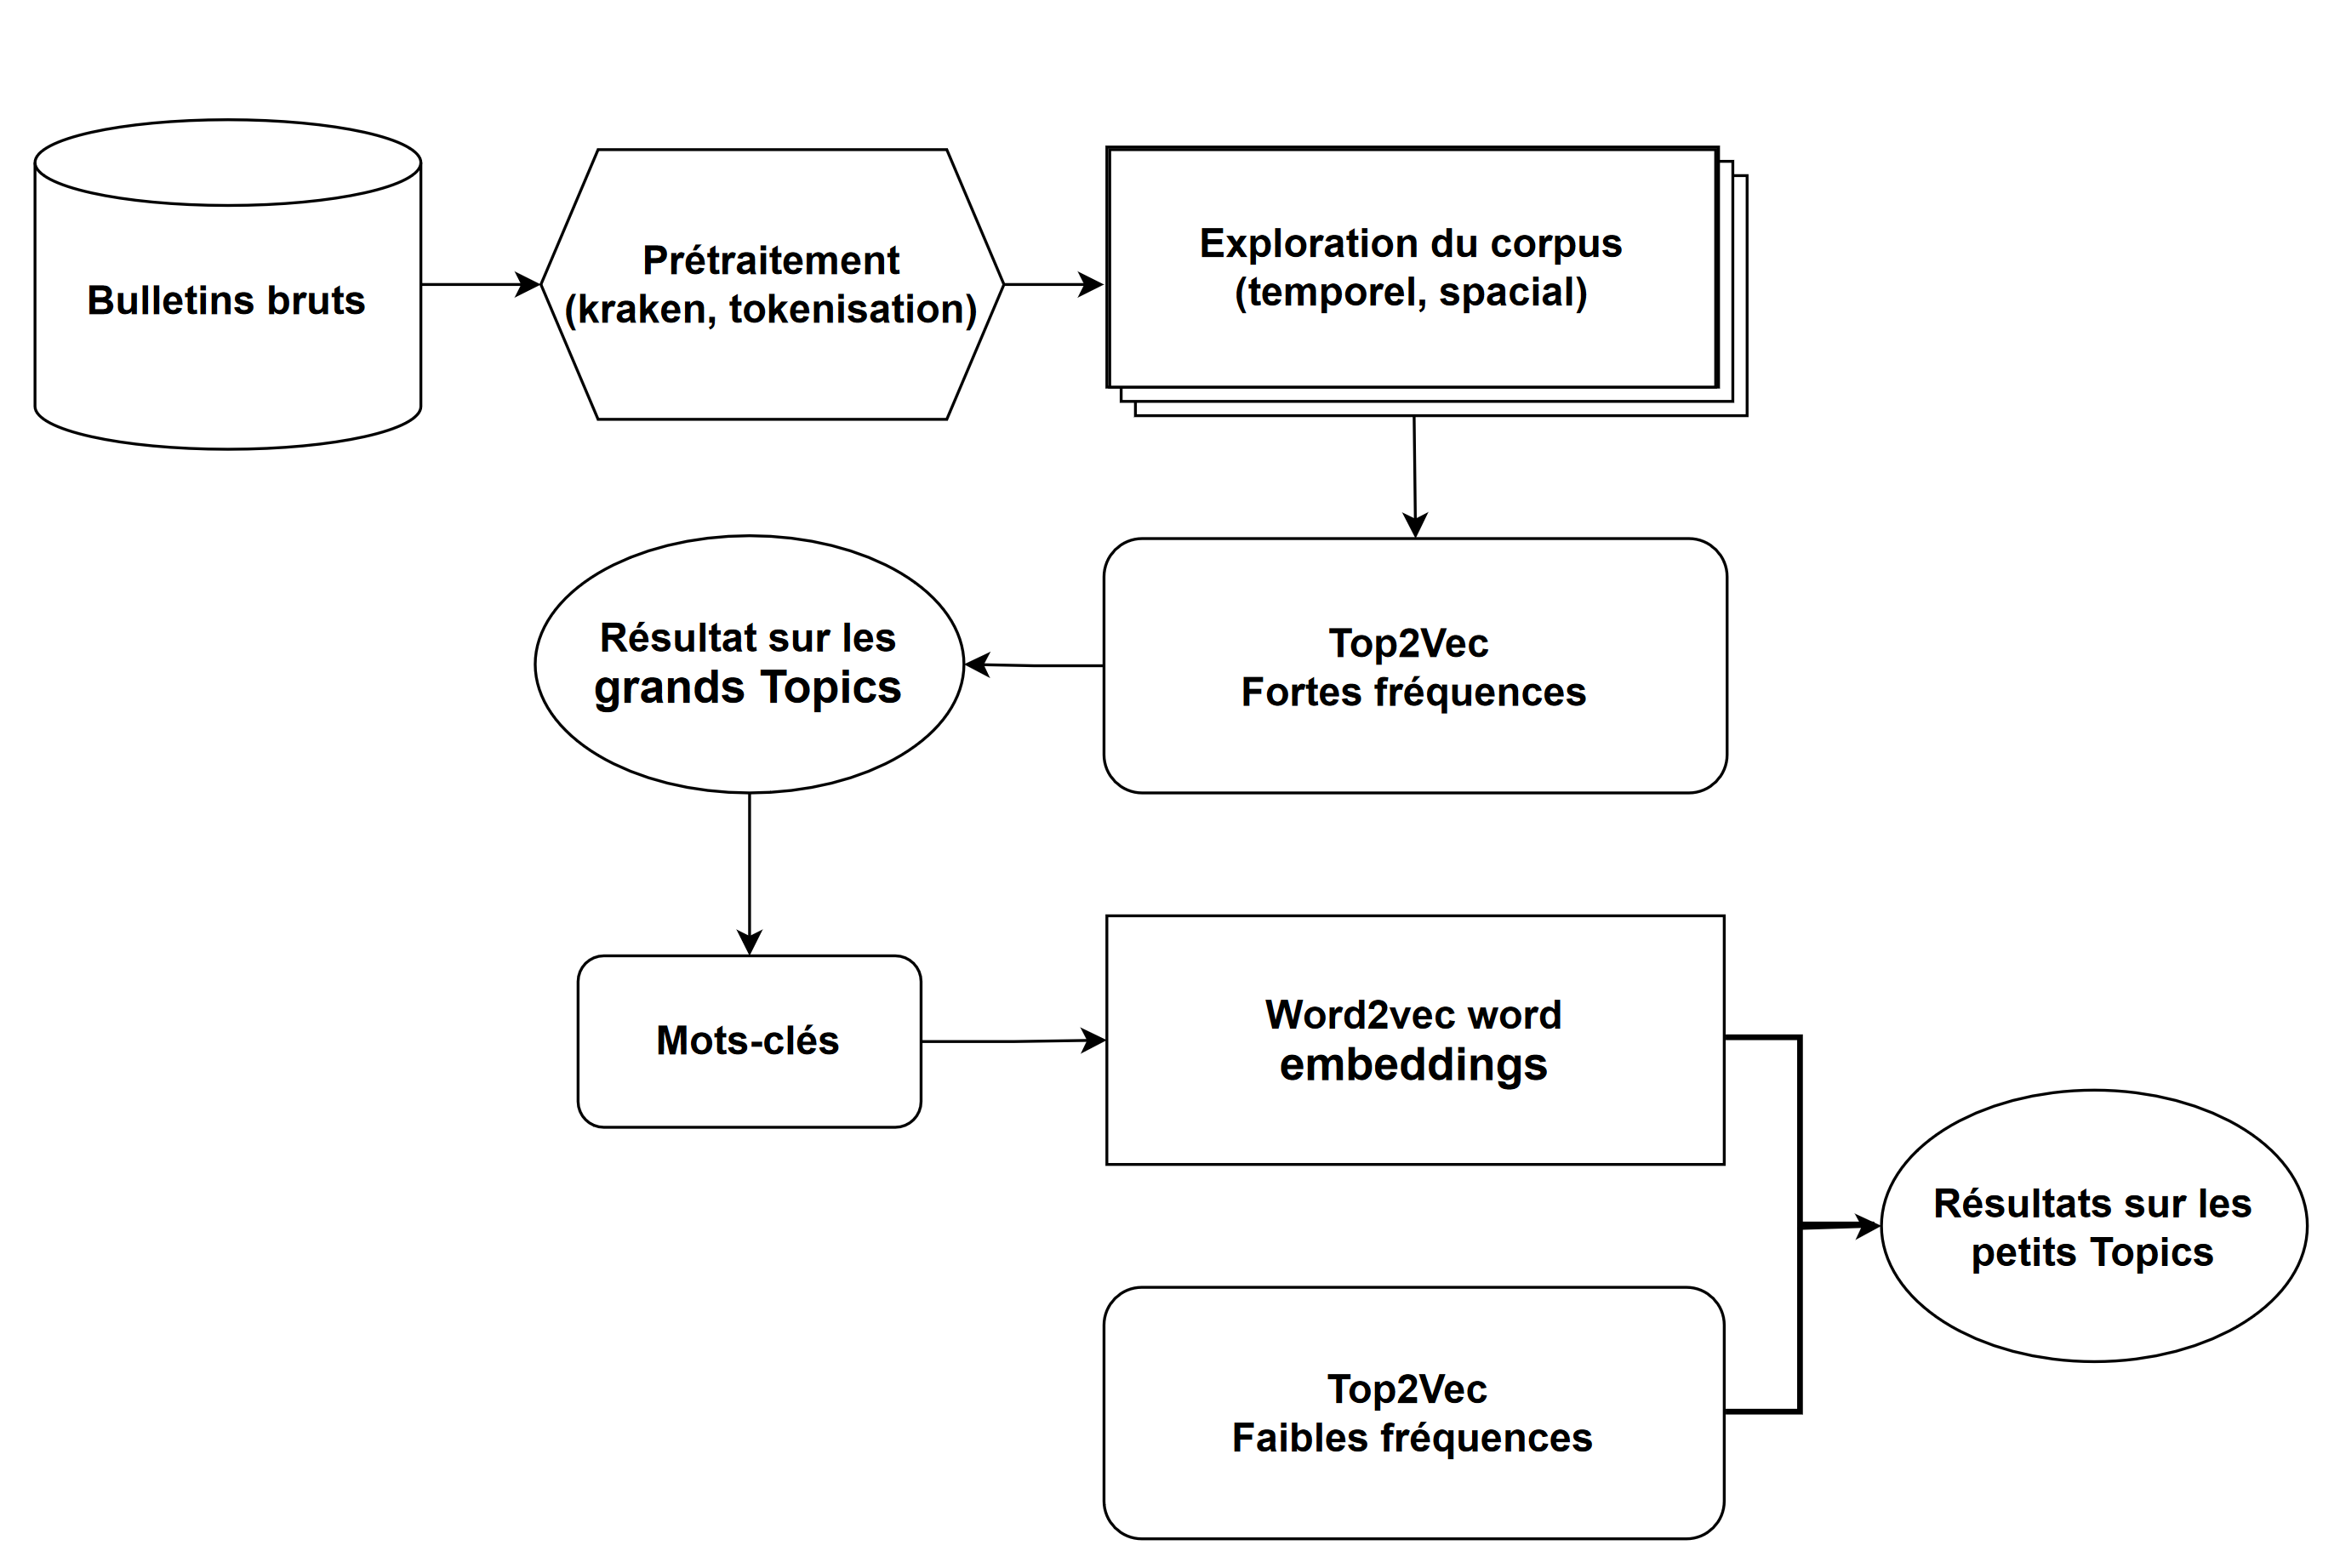
\includegraphics[width=1\linewidth]{img/1.2.diagram.PNG}
    \caption{Diagramme des étapes de travail}
    \label{fig:diagram}
\end{figure}


En premier lieu, le modèle Top2Vec est appliqué aux mots qui apparaissent fréquemment dans le texte, ce qui nous aide à identifier les sujets les plus importants du corpus. Ces sujets sont résumés à l'aide de mots-clés, qui seront ensuite utilisés dans un modèle d'intégration de mots appelé Word2Vec pour créer des ensembles de mots-clés plus détaillés. La combinaison de ces mots-clés avec un modèle Top2Vec entraîné sur des mots à faible fréquence d'occurrence nous permettra d'identifier des groupes de documents contenant des sujets latents à supprimer du corpus.


\part{Exploration du corpus Indochine}

\chapter{Un corpus scientifique important de l'Indochine}

\section{Base de données}

\subsection{Collection des Bulletins de la Société des études Indochinoises}

Le Bulletin de la Société des Études Indochinoises est une publication spécifiquement sélectionnée pour être numérisée dans le cadre du projet VALEASE (Valorisation de l'écrit en Asie du Sud-Est) depuis 2005. Ce projet consiste en une base de données numérique totale qui compte 540.000 pages de texte, soit 5\% des ressources de la Bibliothèque scientifique générale de Hô Chi Minh-Ville. Ce projet fait partie de la Bibliotheca Vietnamica, qui vise à numériser les archives de documents français anciens considérés comme un patrimoine national du Vietnam. L'objectif est de diffuser largement ces documents en Asie du Sud-Est et dans le monde entier. Parmi ces documents, on trouve de nombreuses publications rares des XVIe, XVIIe et XVIIIe siècles, telles que \textit{DelFhistoria della China} (1586), \textit{Dictionarivm annamiticvm lvsitanvm}, et \textit{latinvm ope sacrae congregations de propaganda fide in lvcem editvm AB / Alexandre de Rhodes} (1651), \textit{Voyage du Siam} (1666), \textit{Le grand dictionnaire historique, ou le mélange curieux de l'histoire sacrée et profane de Louis Moréri} (1759), et \textit{Voyage au Tonkin} (1788).

Les revues scientifiques numérisées dans le cadre du projet comprennent: Bulletin des Amis du Vieux Huê (BAVH) (1914-1923), Bulletin de l'École française d'Extrême-Orient (BEFEO) depuis 1901 , la revue Sudia (Van Su Dia) (1969-1975), ect.

Ces sources documentaires sont disponibles, pourtant elles manquent de recherches ultérieures approfondies sur le contenu des documents ainsi que sur les systèmes organisationnels qui les sous-tendent, sur les sujets, les auteurs, les fonctions, la quantité de journaux, les méthodes d'organisation et les institutions financières. Toutes ces informations, issues de documents authentiques, sont utiles pour mieux comprendre l’histoire de l’Indochine.

La qualité des fichiers PDF varie de 300 DPI, ce qui comprend les numéros annuels, soit un total de 82 dossiers avec 164 numéros. Les données des numéros de journaux ont ensuite été compilées manuellement par l'équipe Vietnamica sous la forme d'un fichier Excel qui contient les titres d'articles en français, traduits en deux langues (anglais et vietnamien), les numéros de journaux et les numéros de pages (sur le PDF et les pages sur papier). Les articles sont également divisés en 14 sections, dont la section "Autres" comprend la majorité des numéros divers non catégorisés. Le processus de classification étant effectué manuellement, l'équipe sélectionne uniquement les éléments clairement mentionnés et ne se penche pas sur les genres d'articles scientifiques. Ces paramètres sont nécessaires pour l'étape suivante du traitement, qui consiste à découper les numéros des journaux en fonction des articles. Cette étape est réalisée à l'aide de scripts PHP sur la page source de la bibliothèque électronique et les articles sont regroupés en sections, notamment : 

\begin{itemize}
    \item 15 unités Actes De La Société
    \item 35 unités bibliographies
    \item 10 unités Sociétés Correspondantes
    \item 15 unités Bureau De La Société Des Études Indochinoises
    \item 6 unités catalogues
    \item 12 unités Communications, Congrès et Allocutions
    \item 141 unités Etudes, Notes et Avis
    \item 35 unités Liste des Membres et Assemblées générales
    \item 12 unités Nécrologies
    \item 98 unités Procès-Verbaux
    \item 42 unités publications
    \item 34 unités Rapports et Comptes-rendus
    \item 18 unités Statuts De La Société Des Études Indochinoises
    \item 774 unités Autres
\end{itemize}

Les articles sont ensuite téléchargés dans la bibliothèque numérique du projet Vietnamica à l'adresse : https://revues.vietnamica.online/version2/bsei/

L'état actuel des données pour la réalisation de ce mémoire est que les numéros du bulletin ont été préalablement découpés. Pour passer à l'étape suivante, qui consiste à former un modèle textuel spécifique au corpus via le logiciel Kraken, nous avons sélectionné une liste d'articles pour la transcription manuelle, servant d'échantillons pour le modèle. Dans le but de mettre en œuvre un modèle mixte adapté au corpus, nous avons choisi les critères suivants :

\begin{itemize}
    \item Articles courts, mettant l'accent sur le contenu important (en fonction du titre de l'article).
    \item Des articles provenant de différentes étapes (afin de diversifier les échantillons d'écriture).
    \item Articles multilingues ou purement vietnamiens.
    \item Les fichiers utilisés pour la formation ont été téléchargés directement sur eScriptorium, reconnus par le modèle français automatique du site, puis corrigés manuellement. 

Les annotations ont ensuite été exportées vers le fichier ALTO et ont servi lors de 5 sessions de formation au total :
\end{itemize}

\begin{itemize}
    \item 700 pages de textes en français du B.S.E.I
    \item 400 pages de textes quoc ngu-français du B.S.E.I
    \item 500 pages de quoc ngu d'autres souces
\end{itemize}

\begin{figure}
    \centering
    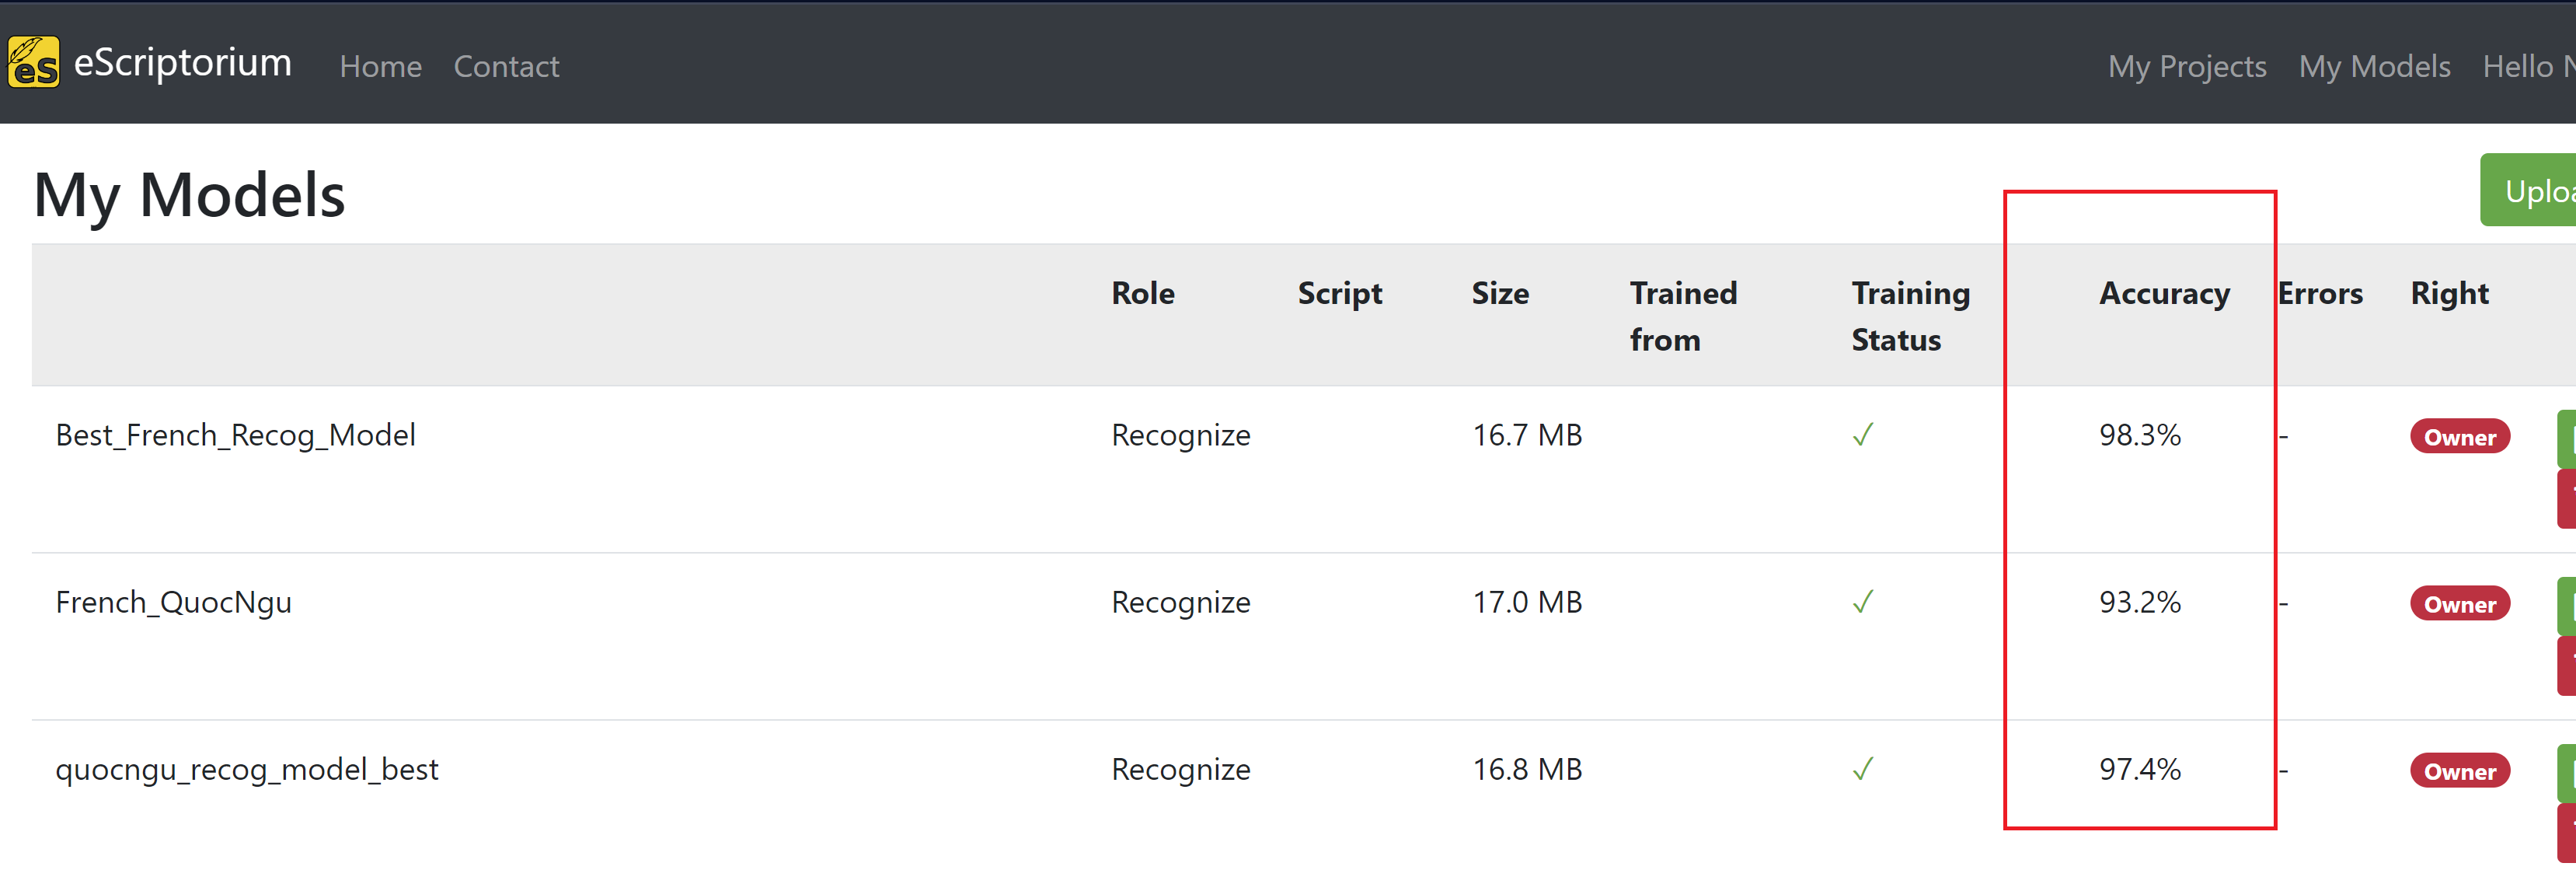
\includegraphics[width=1\linewidth]{img/model3.PNG}
    \caption{Les trois modèles principaux}
    \label{fig:enter-label}
\end{figure}

\textbf{Résultat :} 

\begin{enumerate}
    \item un modèle mixte atteint 93,2\% d'efficacité
    \item un modèle quoc-ngu 97\% d'efficacité
    \item Un modèle français 98.3\% d'efficacité
\end{enumerate}

Nous utilisons le modèle mixte pour exploiter le corpus B.S.E.I dans le cadre de ce projet. Cependant, ce modèle n'est réellement efficace qu'avec le français, et les parties vietnamiennes sont pratiquement inutilisables pour notre exploitation. Cela est en partie dû au faible nombre de textes en vietnamien dans le corpus, ce qui se reflète dans le processus de sélection manuelle des échantillons pour la formation. Avec un corpus comme le B.S.E.I, un modèle ayant une efficacité de 93,2\% est acceptable pour les premières expériences de recherche.

Le corpus du Bulletin de la Société des Études Indochinoises (B.S.E.I) revêt une importance capitale au sein de la bibliothèque numérique Vietnamica. Cette source regroupe un total de 1 342 articles numérisés, tâche entreprise par l'équipe du projet européen Vietnamica, centré sur la recherche historique et la numérisation de documents épitaphes vietnamiens.

De plus, 26 numéros du B.S.E.I sont également consultables dans la bibliothèque Galica, avec leur modèle français atteignant un taux d'efficacité de 87,95\%. À l'heure actuelle, l'intégralité des numéros du Bulletin de la Société des Études Indochinoises est accessible en libre consultation via l'adresse numérique du projet.

Les documents utilisés dans cette étude sont des numéros du B.S.E.I numérisés au format PDF. Le Bulletin a été publié pour la première fois à Saigon en 1883, succédant ainsi au Bulletin du Comité Agricole et Industriel de la Cochinchine (1865-1882). Selon les informations fournies dans le dernier numéro du B.S.E.I datant de 1975, il est possible de distinguer deux étapes cruciales dans le développement de cette publication :

\begin{itemize}
    \item 1883-1823 Ancienne série volumes 1-71 appelée Bulletin de Saigon
    \item  1826-1975 Nouvelle série change son nom pour Bulletin
\end{itemize}
Il convient de noter qu'il manque un numéro daté de 1938 dans le corpus, en raison de contraintes liées à la collecte des données.
\begin{figure}
    \centering
    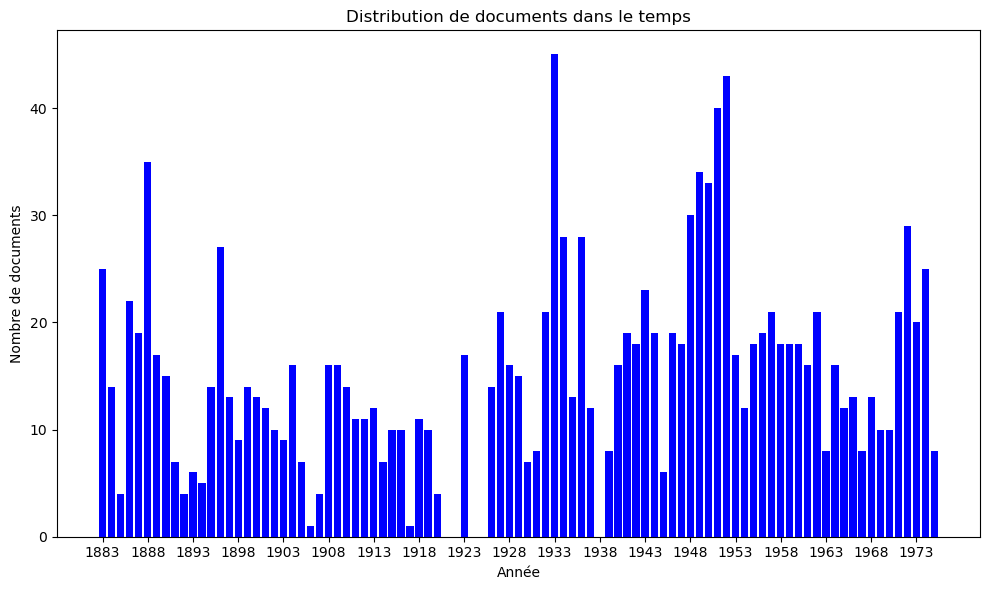
\includegraphics[width=1\linewidth]{img/2.1.nb_doc_year.png}
    \caption{Distribution de documents dans le temps}
    \label{fig:nb_doc_year}
\end{figure}

Parmi ces éditions, il y avait une réédition des volumes de l'édition originale datant de 1974, et ces publications étaient disponibles à la vente dans les bibliothèques correspondantes à Saigon, Hong Kong, Paris, et Bruxelles.

Parmi les volumes du B.S.E.I, deux publications d'une importance particulière ont été extraites et ultérieurement publiées de manière indépendante : 
\begin{itemize}
    \item Les Bas-Reliefs des Urnes Dynastiques de Hue par le R.P Bar-Nouin (1974)
    \item Historique romain des Trois Royaumes (trad. Nghiem Toan et Louis Ricaud) (1960-1963)  
\end{itemize}

Parmi eux, le Roman Historique des Trois Royaumes est réédité chez Flammarion depuis 2009 en France. \footnote{https://editions.flammarion.com/les-trois-royaumes-1/9782081225541}

Pour cette étude, notre attention sera exclusivement portée sur les publications scientifiques majeures du Bulletin de la Société des Études Indochinoises, sans recourir à la numérisation ni à l'utilisation des documents de son prédécesseur, le Bulletin du Comité agricole et industriel de la Cochinchine.

 %%%%%%% IMAGE illustion
 
La source des documents de recherche utilisés est l'une des près de 900 titres multilingues numérisés appartenant à la bibliothèque numérique Vietnamica. Ces documents numériques couvrent de nombreux sujets de la société du Vietnam et de l'Indochine aux XVIIe et XXe siècles, notamment : Arts, loisirs et sports ; Bibliographies, Guides et Annuaire ; Géographie et Histoire ; Institutions, droit et règlements ; Langues ; Littérature ; Monographies ; Religion ; Sciences sociales ; Sciences et techniques… Tous ces documents sont en open source, accessibles à tous pour qu'ils puissent s'y référer et les consulter. Outre les livres, deux importantes collections de journaux scientifiques sont conservées : le Bulletin de la Société des Études Indochinoises, le Bulletin des Amis du Vieux Huê, Excursions et Reconnaissances.

Le jeu de données utilisé pour ce mémoire comprend 164 numéros et constitue l'ensemble le plus complet de documents du B.S.E.I que nous avons pu trouver. Un aperçu de la distribution temporelle des données est présenté dans le tableau ci-dessus.

La Société des Études Indochinoises est la principale société savante parmi toutes les autres sociétés, et le corpus B.S.E.I est le document existant le plus ancien parmi les corpus, il peut donc être considéré comme un corpus précieux. Le B.S.E.I est rédigé en plusieurs langues, notamment le chinois, le quoc-ngu, le laotien, le cambodgien et le français.

Afin de disposer d'un corpus de textes uniforme pour la recherche et dans le but supplémentaire d'avoir un modèle de reconnaissance de texte efficace dans de nombreuses langues, ce qui aidera à numériser de nombreux textes dans la base de données de textes coloniale, nous avons décidé de construire un modèle.

Choix de Kraken 

Nous avons choisi Kraken car nous souhaitions former nous-mêmes un modèle adapté aux documents, notamment multilingues, pouvant inclure des langues non latines comme les caractères chinois et cambodgiens.

\textbf{Étapes d'entraînement :}

Expérience : 1000 pages imprimées saisies à la main, dont la plupart sont en français, avec de nombreuses polices différentes. Le vietnamien est utilisé sur environ 700 pages (à la fois des mots nouveaux et anciens), mais cela s'avère peu efficace. Parce que le nombre de textes en vietnamien dans le corpus B.S.E.I lui-même est encore limité.

Résultats : Le modèle actuel atteint une précision de 93.2\% pour le français et le vietnamien, notamment pour le français, qui est excellent.
Le résultat final consiste donc à utiliser le modèle et à effectuer des recherches en fonction des résultats obtenus.
Envisageons la mise en place d'un moteur de recherche textuelle pour les transcriptions.

\subsection{Méthode de l'extraction de données textuelles}

% Extraction de textes a partir des fichiers numerique (pdf):
% - conversion pdf en images (fichier pdf est de size 1535x2480, 300 DPI)
% - extraire de textes avec kraken
% UNE SOUS-CHAPITRE POUR LE KRAKEN ET L'APPRENTISAGE DU MODELE
\subsubsection{Entraînement du Modèle OCR Kraken}
L'étape importante de ce projet consiste à extraire du texte à partir d'images, et cela est rendu possible grâce à un modèle OCR (Reconnaissance Optique de Caractères en français). L'OCR est un type de modèle d'intelligence artificielle spécialement conçu pour reconnaître et extraire du texte à partir d'images ou de documents scannés. L'objectif principal d'un modèle OCR est de prendre une image contenant du texte, telle qu'une page de livre, un document imprimé ou une photo d'un panneau de signalisation, et de la convertir en texte éditable et lisible par une machine.

Pour notre projet, nous avons développé un modèle OCR en utilisant Kraken, un ensemble d'outils OCR qui permet un entraînement relativement facile pour une grande variété de scripts\footnote{\cite{kraken}}.

La formation d'un modèle OCR (Optical Character Recognition) comporte plusieurs étapes, parmi lesquelles deux sont essentielles : la segmentation et la transcription. La segmentation consiste à diviser une image contenant du texte en régions ou en lignes de texte individuelles. Une segmentation appropriée est essentielle car elle permet de séparer le texte des éléments non textuels et de délimiter chaque élément de texte, facilitant ainsi la reconnaissance et la transcription précise du texte par le modèle OCR. Notre processus de segmentation est réalisé en suivant les étapes suivantes :
\begin{itemize}
    \item Dans un premier temps, nous utilisons un modèle de référence sur Escriptorium pour segmenter les fichiers images
    \item Ensuite, nous corrigeons les segmentations sur Escriptorium, une plateforme collaborative conçue pour la transcription, l'annotation et l'analyse de documents manuscrits et historiques.
    \item Nous sélectionnons ensuite ces images segmentées et les exportons au format ALTO avant de les télécharger sur le serveur 
    \item Nous entamons le processus d'entraînement du modèle en préparant un fichier .sh contenant le script shell nécessaire, que nous exécutons sur le serveur.
\end{itemize}

La transcription, qui suit la segmentation, consiste à reconnaître et convertir les régions ou lignes de texte segmentées en caractères ou mots lisibles par une machine. Cette étape repose sur des techniques d'apprentissage automatique, faisant souvent appel à des réseaux de neurones, pour la reconnaissance et la transcription du texte.

La première phase de la transcription est la construction d'un "ground-truth dataset" (ensemble de données de vérité terrain), qui s'agit un ensemble de données annotées de manière précise et fiable qui sert de référence ou de vérité incontestable dans le domaine de l'apprentissage automatique.

Une fois que ces données sont préparées, nous les exportons sous forme de fichiers ALTO et les téléchargeons sur le serveur. L'entraînement du modèle est réalisé en utilisant les commandes fournies par Ketos, un framework logiciel spécialement conçu pour diverses tâches liées à l'analyse OCR. Ketos fait partie de l'écosystème Kraken OCR et est fréquemment utilisé dans le domaine des humanités numériques. L'ensemble des instructions concernant l'entraînement est décrit sur le site officiel de Kraken.\footnote{https://kraken.re/3.0/ketos.html}

% \textbf{evaluation du modele}

\section{Exploration du corpus}
\subsubsection{Outils de programmation}

Ce travail repose sur le langage de programmation Python ainsi que sur les bibliothèques construites au-dessus.

Pour l'analyse et la manipulation des données, nous faisons usage de Pandas\footnote{https://pandas.pydata.org/} et Numpy\footnote{https://numpy.org/}. Pour le traitement du texte y compris le nettoyage du texte, la tokenisation, nous utilisons les bibliothèques Spacy\footnote{https://spacy.io/} et NLTK\footnote{https://www.nltk.org/}.

Le regroupement des sujets est réalisé avec l'aide de Top2Vec, tandis que l'entraînement du modèle Word Embedding est effectué à l'aide de Word2Vec, une bibliothèque proposée par Gensim.

La visualisation des résultats est réalisée en utilisant des bibliothèques spécialisées dans ce type de tâche, telles que Matplotlib et UMAP.

\subsection{Exploration des titres de documents}

L'analyse des titres de documents peut s'avérer être un point de départ utile lors de l'analyse d'un sujet.

Le titre d'un article dans notre collection de documents comprend généralement le nom de l'article, la période concernée par le sujet ou la personne mentionnée, ainsi que le numéro de tome et/ou de fascicule. Quelques exemples du traitement de titre sont montrés dans le tableau \ref{tab:title_example}. En utilisant des techniques d'expressions régulières, nous procédons à l'extraction des mots vides ou des mots peu pertinents, tels que le numéro de tome ou de fascicule, afin de ne conserver que les termes importants du document. Nous nous intéressons à l'année de parution du document qui est systématiquement placée en dernière position et séparée par un tiret bas.

\begin{tabularx}{\textwidth}{X|l|l}
  \textbf{Titre original} & \textbf{Titre normalisé} & \textbf{Année} \\
\hline
 {actes-de-la-société\_1949\_tome\_xxiv\_3} &  acte société & 1949\\ 
\hline
    {un-cas-de-droit-maritime-international-en-1797\_1948\_tome\_xxiii} &  cas droit maritime international & 1948 \\
\hline
    {charles-carpeaux-1870-1904\_1952\_tome \_xxvii} & charles carpeaux& 1952 \\ 
    \label{tab:title_example}
\end{tabularx}

La période couverte du corpus s'étend sur deux siècles, de 1883 à 1975, comme illustré dans la Figure \ref{fig:nb_doc_year}. La répartition temporelle met en évidence le développement de la société au fil du temps, notamment pendant la période d'installation du colonialisme français en Indochine au début et le partie suivante en plein développement de la revue  malgré les contextes politiques complexes. Il est à noter qu'il existe une coupure dans les données autour des années 1920, due à la période de transition du Bulletin, marquant ainsi la séparation des deux parties du corpus.

Les collocations dans les titres sont visualisées dans la Figure \ref{fig:bigram-title}. On peut observer que les articles portant sur les études de la société indochinoise sont particulièrement plus fréquents que les autres. De plus, les actes de sociétés et les procès-verbaux sont également très présents dans le corpus.
\begin{figure}
    \centering
    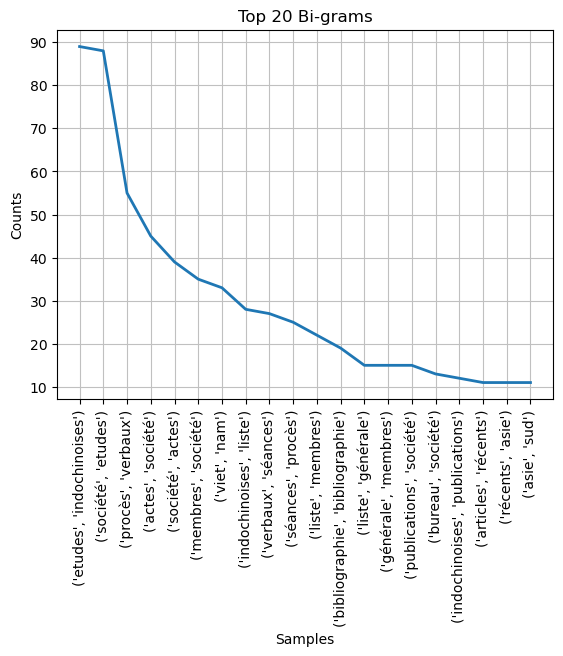
\includegraphics[width=12cm]{img/2.2.bigram-title.png}
    \caption{Bigram par titres}
    \label{fig:bigram-title}
\end{figure}

Un nuage de mots est une représentation visuelle de données textuelles qui est utilisée pour mettre en évidence les mots les plus fréquents dans un texte ou un corpus donné. C'est une technique de visualisation de données populaire qui offre un moyen rapide et intuitif de comprendre les termes ou les mots clés présents dans un ensemble de données.

\begin{figure}
    \centering
    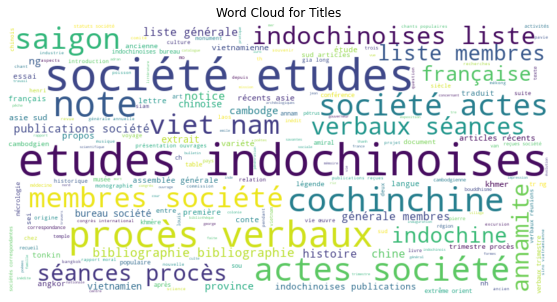
\includegraphics[width=12cm]{img/2.3.word_cloud_title.png}
    \caption{Nuage de mots par titres}
    \label{fig:nuage_titre}
\end{figure}

Le nuage de mots pour les titres est présenté dans la Figure \ref{fig:nuage_titre}, ce qui nous donne une idée des principaux sujets abordés dans le corpus. Comme pour les n-grams, cette visualisation nous permet de constater que les "études indochinoises" sont un thème récurrent dans l'ensemble des publications.

Un graphe de co-occurrence, également appelé réseau de cooccurrence ou matrice de cooccurrence, est un concept fondamental du NLP. Il est utilisé pour représenter et analyser les relations entre les éléments en fonction de leur cooccurrence dans un ensemble de données.

\begin{figure}[H]
    \centering
    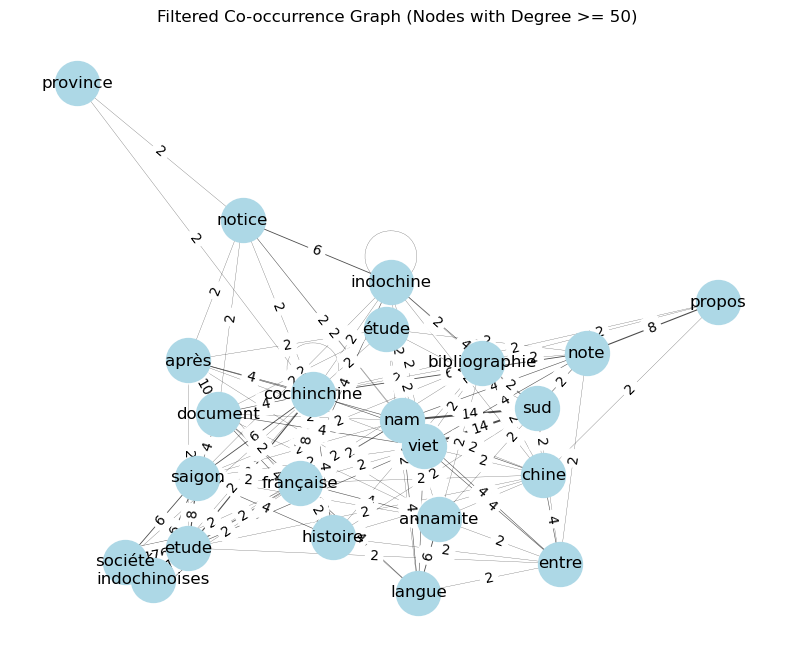
\includegraphics[width=12cm]{img/2.4.co-occurence-title.png}
    \caption{Graphe co-occurrence}
    \label{graph_cooc}
\end{figure}

Les mots qui co-apparaissent fréquemment sont susceptibles d'être sémantiquement liés, ce qui permet d'obtenir un aperçu de la structure sous-jacente du texte. Dans le cas de votre exemple avec les mots "étude", "société", et "indochinoise", on peut intuitivement constater que ces sujets sont liés à des termes tels que "Saigon", "français" et "histoire".


%%%%%%%%%%%%%%%%%%%%%%%%%%%%%%%%%%%%%%%%%%%%%%%%%%%%%%%%%%%%%%%%%%%%%%%%%%%%%%%%%%%%%%%%%%%%%%%%%%%%%%%%%%%%%%%%%%%%%%%%%%%%%%%%%%%%%%%%%%%%%%%%%%%%%%%%%%%%%%%%%%%%%%%%%%%%%%%%%%%%%%%%%%%%%%%%%%%%%%%%%%%%%%%%%%%%%%%%

\subsection{Exploration générale du corpus}
\subsubsection{Statistiques du Corpus}
Le tableau \ref{Tab:statscorpus} présente une description avec les statistiques simples de la taille du corpus.

\begin{table}[H]
\caption{Statistiques du corpus}
\centering
\bigskip
\begin{tabular}{lc}
    \hline
    Article &  916 \\
    Phrases &  474034  \\
    Mots &  6345322 \\
    \hline
\end{tabular}
 \label{Tab:statscorpus}
\end{table}
\bigskip

Les bigrammes et trigrammes du corpus sont visualisés dans la figure \ref{fig:bigram}. On y retrouve les collocations déjà rencontrées dans les titres, telles que "étude indochine", "procès verbal", "membre société", ainsi que des collocations plus spécifiques comme "extrême orient", "point vue", "phan thanh gian", etc.

\begin{figure}
\centering
\begin{subfigure}{0.6\textwidth}
    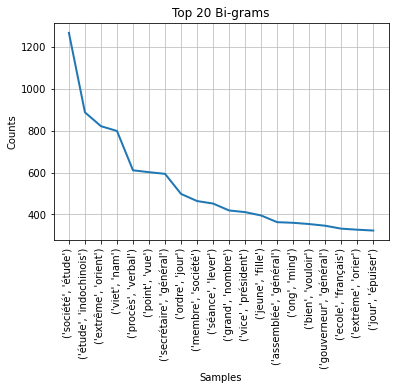
\includegraphics[width=\textwidth]{img/2.5.bigram.png}
    \caption{Bigrams}
    \label{fig:bigram}
\end{subfigure}
\hfill

\begin{subfigure}{0.6\textwidth}
    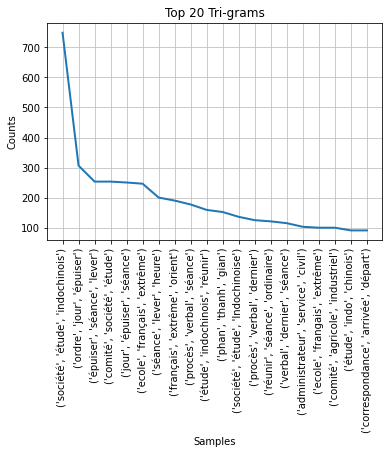
\includegraphics[width=\textwidth]{img/2.6.trigram.png}
    \caption{Trigrams}
    \label{fig:trigram}
\end{subfigure}
        
\caption{Collocations populaires du corpus}
\label{fig:ngrams}
\end{figure}
    
Dans la figure \ref{fig:nuage_corpus}, nous présentons un nuage de mots du corpus. Il est important de noter que les verbes les plus courants ont été exclus pour mettre en évidence les termes les plus intéressants :

\begin{figure}[H]
    \centering
    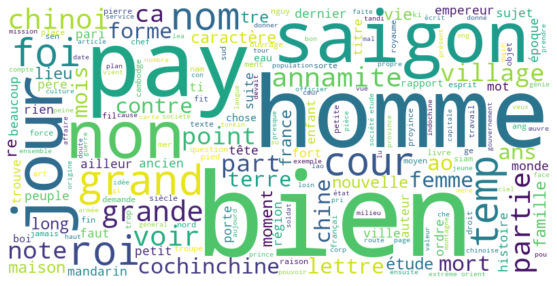
\includegraphics[width=12cm]{img/2.7.word_cloud_total.png}
    \caption{Nuages des mots du corpus}
    \label{fig:nuage_corpus}
\end{figure}

%%%%%%%%%%%%%%%%%%%%%%%%%%%%%%%%%%%%%%%%%%%%%%%%%%%%%%%%%%%%%%%%%%%%%%%%%%%%%%%%%%%%%%%%%%%%%%%%%%%%%%%%%%%%%%%%%%%%%%%%%%%%%%%%%%%%%%%%%%%%%%%%%%%%%%%%%%%%%%%%%%%%%%%%%%%%%%%%%%%%%%%%%%%%%%%%%%%%%%%%%%%%%%%%%%%%%%%%%%%%%%%%%%%%%%%%%%%%%%%%%%%%%%%%%%%%%%%%%%%%%%%%%%%%%%%%%%%%%%%%%%%%%%%%%%%%%%%%%%%%%%%%%%%%%%%%%%%%%%%%%%%%%%%%%%%%%%%%%%%%%%%%%%%%%%%%%%%%%%%%%%%%%%%%%%%%%%%%%%%%%%%%%%%%%%%%%%%%%%%%%%%%%%%%%%%%%%%%%%%%%%%%%%%%%%%%%%%%%%%%%%%%%%%%%%%%%%%%%%%%%%%%%%%%%%%%%%%%%%%%%%%%%%%%%%%%%%%%%%%%%%%%%%%%%%%%%%%%%%%%%%%%%%%%%%%%%%%%%%%%%%%%%%%%%%%%

\subsubsection{Suppression des mots vides}
La suppression des mots vides des données textuelles dans NLP offre plusieurs avantages, notamment la réduction du bruit, la réduction de la dimensionnalité et l'augmentation de la sensibilité aux termes importants. 
Un comptage a été mis en place pour estimer la proportion de mots vides dans le texte original, et il s'avère qu'ils représentent environ 4.12\% de l'ensemble du corpus.

Comparé à la liste des mots vides de NLTK, celle fournie par Spacy est plus complète, nous l'utilisons pour les analyses de modélisation de sujets qui nécessitent la suppression maximale des mots peu importants. Voici un exemple pour illustrer comment les mots vides sont supprimés en utilisant les listes de mots vides de Spacy et de NLTK :

\textbf{Texte original} : \textit{des liens sociaux des coutumes et des mœurs des religions et des philosophies qui commandent les cohésions et les poussées populaires étude des sciences et des littératures qui nourrissent intellectuellement les élites dirigeantes apparaissent de plus en plus nécessaires notre époque tous les peuples frémissent et ébranlent vers des destins nouveaux. Les débuts de étude systématique de extrême orient et le défrichement des sciences humaines d' asie ne datent que d'hier. et bon nombre des études faites commencent à peine à être diffusées. or la société des etudes indochinoises a le privilège plus rare dans le monde entier qu' on ne pense utiliser les concours de savants et de spécialistes qui ont une expérience directe des pays et des civilisations extrême}

\textbf{Texte traité par NLTK}: \textit{ lien social coutume mœur religion philosophie commander cohésion poussée populaire    étude science littérature nourrir intellectuellement élite dirigeant apparaître plus plus nécessaire    époque    tout peuple frémir    ébranlent vers destin nouveau début    étude systématique    extrême orient défrichement science humain    asie dater    hier bon nombre étude fait commencer    peine    être diffuser or société etude indochinoise avoir privilège plus rare monde entier penser    utiliser concours savant spécialiste avoir expérience direct pays civilisation extrême}

\textbf{Texte traité par Spacy} : \textit{ lien social coutume mœur religion philosophie commander cohésion poussée populaire    étude science littérature nourrir intellectuellement élite dirigeant apparaître nécessaire    époque    peuple frémir    ébranlent destin début    étude systématique    extrême orient défrichement science humain    asie dater    hier bon nombre étude commencer    peine    diffuser société etude indochinoise privilège rare monde entier penser    utiliser concours savant spécialiste expérience direct pays civilisation extrême.}
%%%%%%%%%%%%%%%%%%%%%%%%%%%%%%%%%%%%%%%%%%%%%%%%%%%%%%%%%%%%%%%%%%%%%%%%%%%%%%
\subsubsection{Analyse de sentiment}

Effectuez une analyse des sentiments pour évaluer le sentiment général ou les émotions exprimées dans le corpus de texte. J’utilise TextBlob un bibliothèque populaire dans ce domaine.

\textbf{Polarité:} La polarité fait référence au ton émotionnel ou au sentiment exprimé dans un morceau de texte. Il indique si le texte exprime un sentiment positif, négatif ou neutre.  La polarité est généralement mesurée sur une échelle numérique allant de -1 à 1, où  -1 représente un sentiment fortement négatif, 0 représente un sentiment neutre et 1 représente un sentiment fortement positif. Par exemple, un texte contenant des mots positifs comme « heureux », « amour » et « incroyable » aura un score de polarité positif. Un texte contenant des mots négatifs comme « triste », « haineux » et « décevant » aura un score de polarité négatif. Un texte contenant un mélange de mots positifs et négatifs peut avoir un score de polarité proche de 0, indiquant un sentiment neutre.

\begin{figure}[!ht]
    \centering
    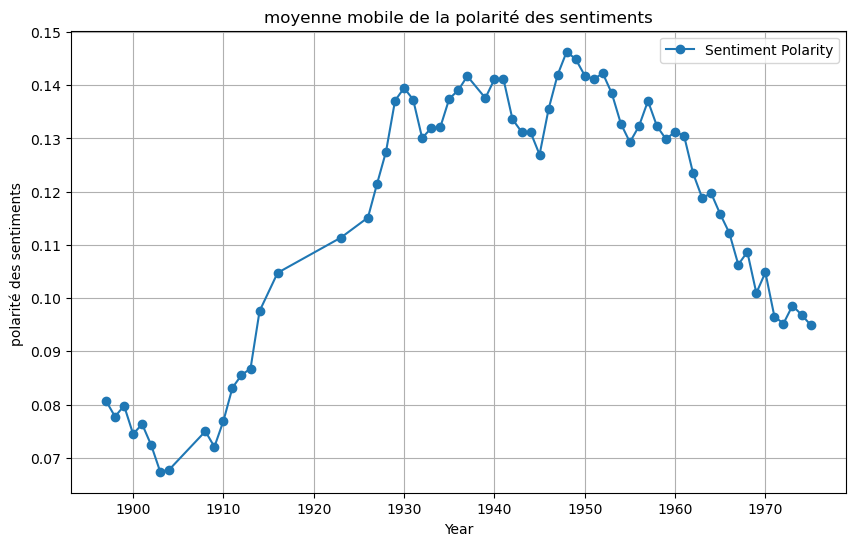
\includegraphics[width=12cm]{img/2.8.polarity_sentiment.png}
    \caption{Nuages des mots des titres}
    \label{fig:polar_senti}
\end{figure}

En général, les scores de polarité des documents sont assez faibles, variant entre 0.07 et 0.15, ce qui indique un sentiment plutôt neutre dans l'ensemble du corpus. Cela peut s'expliquer par le fait que les documents sont principalement des bulletins d'études, qui ont tendance à être informatifs et à contenir peu d'émotion. Cependant, on peut observer une augmentation continue de la polarité entre 1880 et 1940. Cette période a été témoin d'une influence coloniale importante en Indochine, principalement de la part des puissances coloniales françaises. Les sentiments exprimés dans le corpus peuvent refléter l'évolution des sentiments de la population locale, passant de la résistance initiale et du mécontentement sous le régime colonial à l'émergence des premiers mouvements nationalistes. Les sentiments pourraient devenir plus positifs à mesure que les gens commençaient à rechercher une plus grande autonomie. Ensuite, on observe la période pendant laquelle le gouvernement colonial français a commencé à se retirer d'Indochine, et en même temps, les nuances expressives des documents ont diminué pour atteindre un état plus neutre.

\textbf{Subjectivité} est la mesure dans laquelle un morceau de texte exprime un point de vue subjectif ou objectif. Cela indique à quel point le texte est basé sur des opinions, des sentiments ou des croyances personnelles plutôt que sur des faits ou des objectifs purement objectifs. La subjectivité est généralement mesurée sur une échelle numérique allant de 0 à 1, où 0 représente un texte très objectif ou factuel et 1 représente un texte hautement subjectif ou basé sur une opinion. Par exemple, un reportage objectif qui présente des faits et des chiffres sans opinions personnelles aura un faible score de subjectivité (proche de 0). Alors qu'un article de blog personnel ou une critique de produit exprimant des sentiments et des opinions personnels auront un score de subjectivité élevé (plus proche de 1).

Le changement de subjectivité des sentiments dans les documents de 1880 à 1975 peut être attribué à des facteurs historiques, politiques et socioculturels qui ont façonné le récit et les attitudes au fil du temps.

\begin{figure}[!ht]
    \centering
    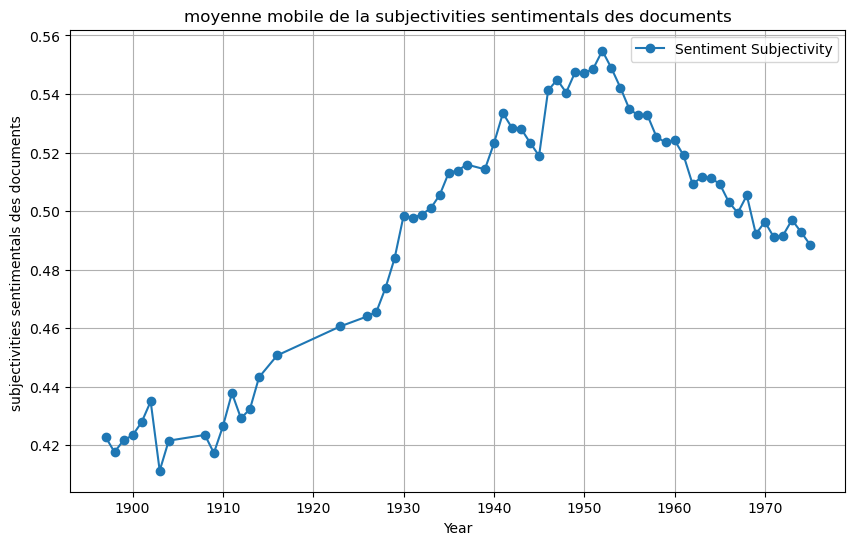
\includegraphics[width=12cm]{img/2.9.subjectivity_sentiment.png}
    \caption{Subjectivite sentimental}
    \label{fig:subject_senti}
\end{figure}

\textbf{Conclusion : }Analyser les sentiments au fil des années dans un corpus lié à l’Indochine peut être significatif pour les études historiques et culturelles. Cependant, elle doit être menée avec une orientation de recherche claire, en étant consciente des limites de l’analyse des sentiments et en tenant compte du contexte historique plus large. Les enseignements tirés d’une telle analyse peuvent contribuer à une meilleure compréhension de la façon dont l’Indochine a été perçue et représentée au fil du temps. 

 Les point de vue de Thomas Kuhn est "On  concevait  qu’en  ajoutant des résultats aux théories, on devrait se rapprocher toujours plus  du  vrai  au  fur  et  à  mesure  des  siècles.  Selon  Kuhn,  cela  ne  se  passe pas ainsi. Le progrès scientifique procède par une succession de périodes calmes et de ruptures. Pendant les périodes stables, la discipline se  développe,  organisée  autour  d’un  paradigme  dominant,  sorte  de  cadre théorique auquel adhère la communauté des professionnels du moment. Par exemple, la mécanique newtonienne a fonctionné ainsi du xviie siècle au début du xxe siècle sans être remise en cause. On y accumule des connaissances, mais aussi des problèmes à résoudre. Lorsque ces anomalies se multiplient, une crise survient, qui peut déboucher  sur  une  révolution  scientifique."\footnote{\cite{thomaskun08}}

 
\subsubsection{Analyse du vocabulaire des termes significatifs}

L'utilisation du terme "Annamite" jusqu'en 1948 dans la Figure \ref{fig:ananm_viet} reflète l'influence de la colonisation française sur la région et l'évolution politique et sociale qui a conduit à l'adoption du terme "Vietnamien" pour décrire le peuple et la nation du Vietnam. Les autorités coloniales françaises avaient une influence considérable sur la région et ont imposé leur propre terminologie et leur vision du monde aux habitants de la colonie. Le terme "Annamite" était historiquement utilisé pour désigner les habitants de la région qui correspond approximativement au nord et au centre du Vietnam moderne. Il provient du nom de l'ancien royaume d'Annam, qui existait avant la colonisation française. Les Français ont conservé ce terme pour désigner les Vietnamiens même après avoir élargi leur contrôle sur l'ensemble de l'Indochine. Le passage de l'utilisation du terme "Annamite" à "Vietnamien" en 1948 a coïncidé avec le déclin du colonialisme français en Indochine et le début du mouvement nationaliste vietnamien dirigé par Ho Chi Minh. Le changement de terminologie était également lié à la montée du nationalisme vietnamien et à l'affirmation de l'identité nationale vietnamienne distincte.

\begin{figure}[H] %[!ht]
    \centering
    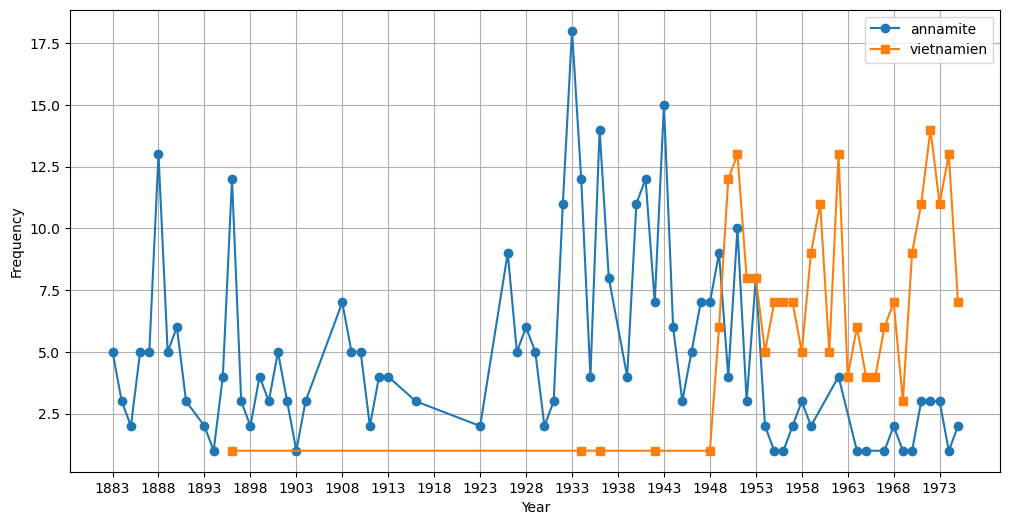
\includegraphics[width=12cm]{img/vietnam_annamite.png}
    \caption{Changement de fréquence d'utilisation entre les termes "annamite" et "vietnamien"}
    \label{fig:ananm_viet}
\end{figure}

On peut clairement observer un changement significatif dans la fréquence d'utilisation de ces deux termes dans la Figure \ref{fig:ananm_viet}. Tout d'abord, vers 1949, le terme "Vietnamien" émerge soudainement avec une utilisation plus répandue. Historiquement, en juillet 1949, le gouvernement provisoire de l'État du Vietnam a été établi, avec la nomination de Bao Dai en tant que chef de l'État. À partir de ce moment, le terme "vietnamien" a été rétabli officiellement. 

M. Cao-vân-Chiêu, ancien conseiller de l'Union Française lorsqu'il demanda, le 3 décembre 1953, à la tribune de l'assemblée versaillaise, que l'adjectif « vietnamien » fût substitué, dans tous les cas, à celui d'annamite qui réapparaissait parfois par inadvertance dans les textes officiels français. » 

Les deux termes, "vietnamien" et "annamite", représentent en réalité deux affirmations totalement différentes de l'identité nationale. Dans le contexte colonial, le terme "annamite" était souvent considéré comme péjoratif, même si, selon Jean Rispaud : 

« En tout cas, avant la deuxième guerre mondiale, les se nommaient eux-mêmes « gens d'Annam » et pas autrement, bien que ce nom sonnât désagréablement aux oreilles des lettrés qui en connaissaient l'origine. Tous les Occidentaux ont pu l'entendre comme moi en Indochine et d'innombrables témoignages écrits le confirment. »\footnote{\cite{vietnam}}

Un curieux problème historique : 
"An Nam" est un ancien nom du Vietnam, qui signifie "Sud Pacifié" et « qui avait été imposé par la Chine  en l'an 264 avant J.-C »\footnote{\cite{vietnam}}. à une époque où le pays était sous la domination du Nord. Ce nom avait pour intention de rappeler la vassalité du Vietnam envers la Chine, car le pays ne s'était pas rebellé ni n'avait fait la guerre. En revanche, le terme "Vietnam" (pays du Sud) affirmait l'indépendance du pays en tant qu'entité distincte, libre de toute colonisation.

Dans les années qui ont suivi, de 1933 à 1949, le terme "annamites" était largement utilisé dans la revue. Cela s'explique en partie par la période florissante du développement de la revue, caractérisée par un grand nombre de textes, ainsi que par la présence d'éminents intellectuels en tant qu'auteurs. Cette période a vu une augmentation des études sur le peuple vietnamien, ses coutumes et ses ethnies par rapport aux années précédentes.

Il est également intéressant de noter qu'à la dernière étape de l'élaboration du bulletin, de 1969 à 1975, le terme "annamites" a progressivement disparu au profit du terme "vietnamien". Cette évolution correspondait aux changements politiques de l'époque, où les Français n'avaient plus l'avantage. De plus, au sein du journal, de nombreux auteurs vietnamiens écrivaient sur leur propre pays et aspiraient à développer une identité nationale et scientifique pour le peuple vietnamien. Par exemple, certains articles d'auteurs vietnamiens en 1971-1972 reflétaient cette évolution.

\begin{itemize}
    \item L’expérience poétique et l’itinéraire spirituel de Han Mac Tu par Vo Long Te (1971)
    \item Quelques livres récents sur les études Vietnamien par Nguyen The Anh (1971)
    \item Nguyen Binh Khiem porte-parole de la sagesse populaire par Xuan Phuc (1971)
    \item Folklore du Sud du Vietnam : ong Hong, l’homme le plus riche de Nam Ky par Dao Van Hoi (1971)
    \item Dictionnaires vietnamiens par Vo Tong Le (1972)
    \item Nguyen Truong To, patriote réformiste, poète et homme d’action par Thai Van Kiem (1972)
    \item Enrichissement des forêts de conifères par introduction d’essences résineuses exotiques sur les Hautes Plateaux du Langbiang par Nguyen Van Thon (1972)
    \item Le culte de la Baleine par Thai Van Kiem (1972)
\end{itemize}

\begin{figure}[H] %[!ht]
    \centering
    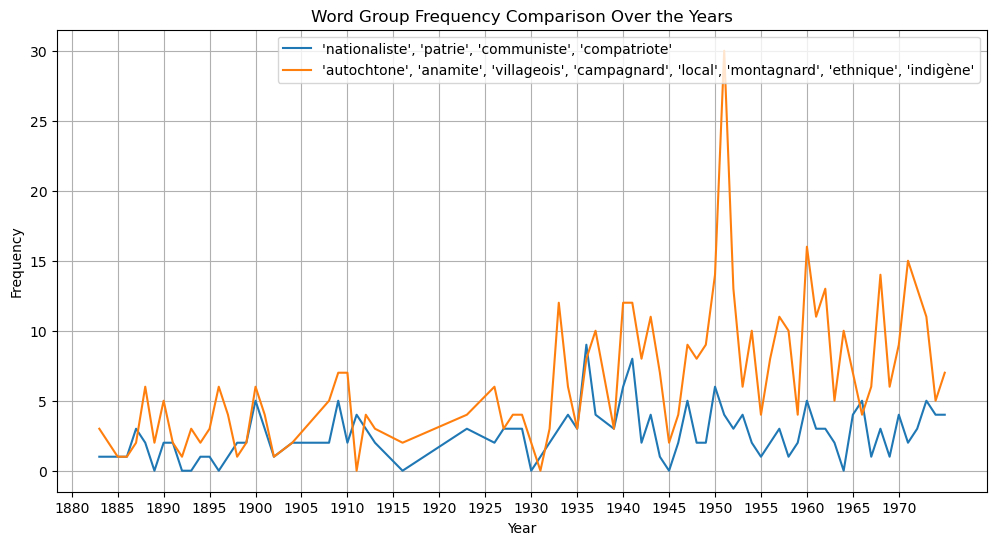
\includegraphics[width=12cm]{img/2.11.national_local.png}
    \caption{Évolution de la fréquence d'utilisation des termes "nationalisme" ou "localisme"}
    \label{fig:national_local}
\end{figure}
Nous portons également notre attention sur des sujets controversés afin de mesurer le niveau d'objectivité du corpus dans la figure \ref{fig:national_local}. Cependant, en ce qui concerne les thèmes liés au localisme, bien que les termes utilisés semblent parfois renvoyer à des minorités ethniques ou à des civilisations moins avancées, ils demeurent un élément récurrent dans l'ensemble du corpus. Les articles correspondants traitent souvent de questions d'ethnicité et d'ethnologie. De même, le nationalisme est abordé plus tard dans le corpus, mais la majorité des articles restent axés sur les études des pays indochinois et leurs aspects ethniques. La quantité accrue d'articles et l'expérience plus approfondie des auteurs entraînent également une augmentation du nombre de mots abordant ces sujets.

\begin{figure}[H] %[!ht]
    \centering
    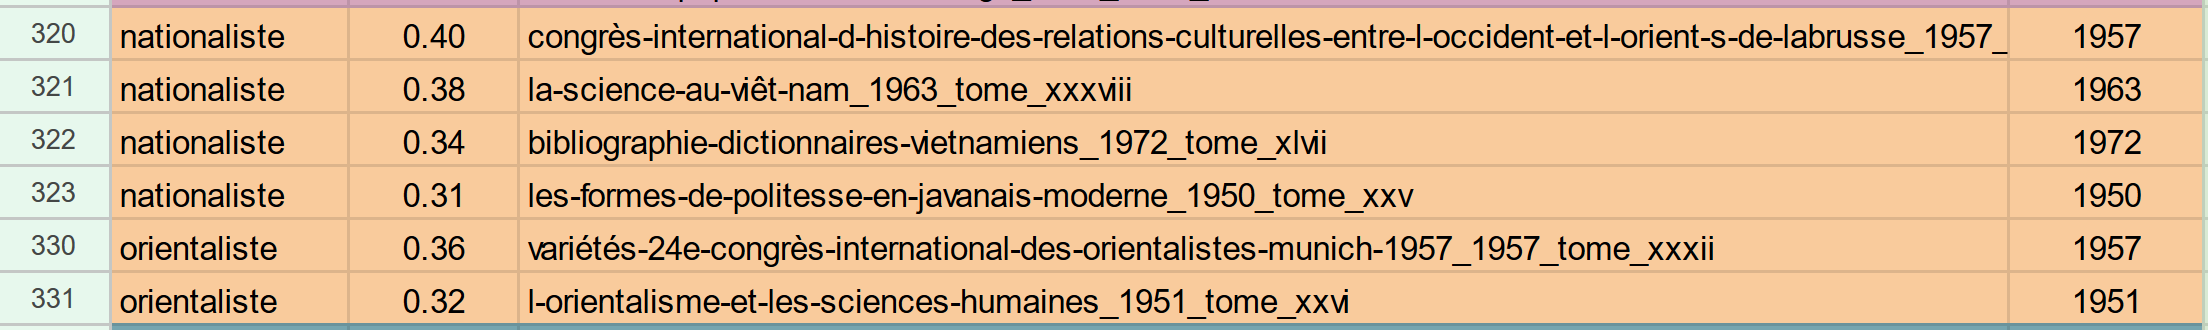
\includegraphics[width=1\linewidth]{img/nationaliste.PNG}
    \caption{Quelques exemples d'articles}
    \label{fig:enter-label}
\end{figure}

\begin{figure}[H] %[!ht]
    \centering
    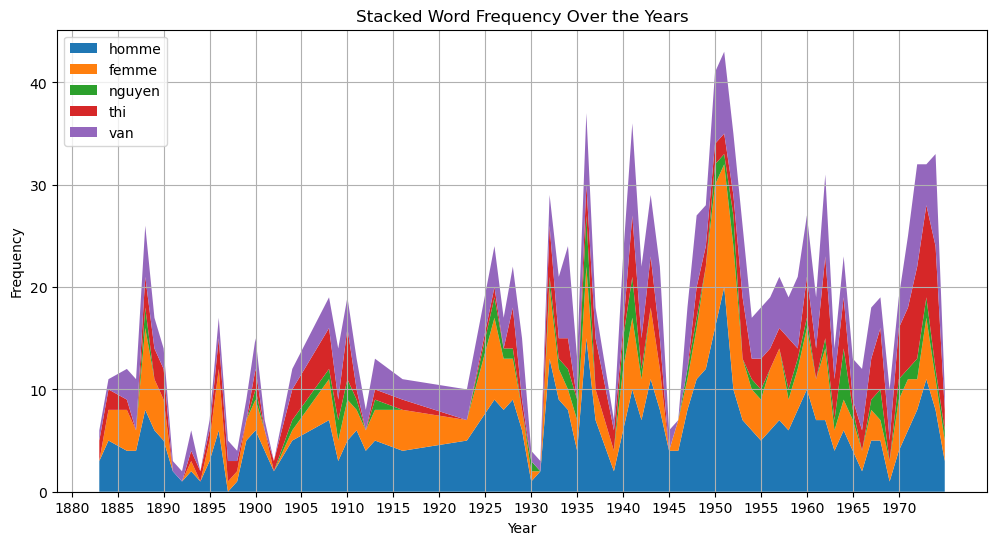
\includegraphics[width=12cm]{img/2.12.name_viet.png}
    \caption{Évolution de la fréquence d'utilisation des termes "homme", "femme" et des noms Vietnamiens}
    \label{fig:name_viet}
\end{figure}


Dans la Figure \ref{fig:mot_geo}, nous analysons l'utilisation de termes géographiques dans différentes régions de l'Indochine. Nous remarquons une répartition très équilibrée de la fréquence d'utilisation de ces termes, ce qui suggère que les publications du bulletin étaient équitablement réparties entre les différentes régions de l'Indochine à l'époque.

Le Tonkin et la Cochinchine étaient deux régions historiques situées dans l'ancienne Indochine française, en Asie du Sud-Est. 
Le Tonkin était situé au nord de l'actuel Vietnam.
Il était délimité approximativement par la rivière Rouge (Song Hong) au nord et par le 17e parallèle au sud, ce qui le séparait de la Cochinchine.
Le Tonkin comprenait les régions du delta du fleuve Rouge et des montagnes du Nord, et il était principalement peuplé par des Vietnamiens Kinh. Hanoï était la capitale du Tonkin.
La Cochinchine était située au sud de l'actuel Vietnam.
Elle était bordée par la mer de Chine méridionale à l'est, le Cambodge à l'ouest, et le Tonkin au nord. La Cochinchine était composée en grande partie de terres basses, y compris le delta du Mékong, et elle était connue pour sa fertilité. Sa principale ville était Saïgon, qui est aujourd'hui Ho Chi Minh-Ville.

\begin{figure}[H]
    \centering
    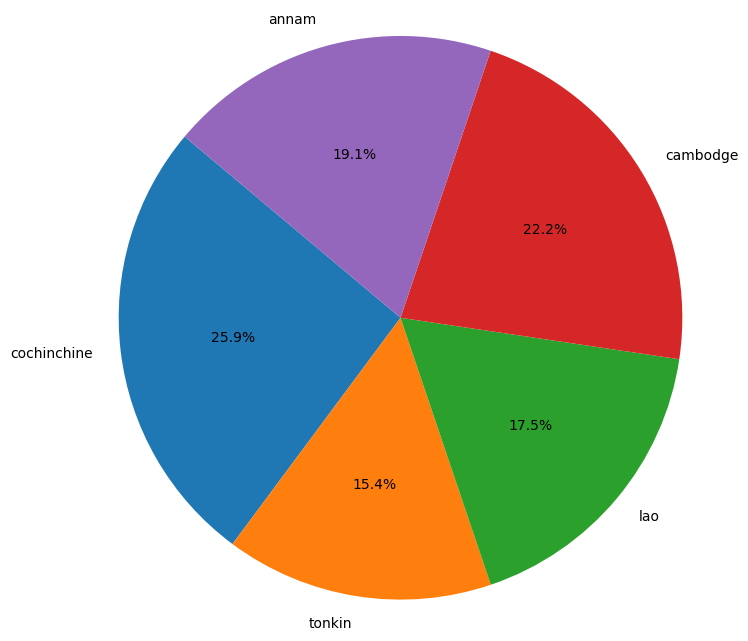
\includegraphics[width=12cm]{img/2.13.mot_geo.png}
    \caption{Répartition des termes des régions géographiques}
    \label{fig:mot_geo}
\end{figure}

Le Laos était l'une des composantes de l'Indochine française. Il était principalement considéré comme une région rurale et montagneuse, et son économie reposait sur l'agriculture, en particulier la culture du riz. Sous la domination française, le Laos a été intégré dans l'administration coloniale indochinoise, bien qu'il ait conservé une certaine autonomie locale. Pendant cette période, le Laos a été exposé à l'influence culturelle française, mais il est resté largement rural et peu développé sur le plan économique.

Le Cambodge, quant à lui, était une autre composante de l'Indochine française. Le Cambodge a une histoire riche et ancienne en tant que royaume khmer, mais il est devenu un protectorat français au XIXe siècle. Pendant la période coloniale, le Cambodge a été gouverné par une administration française, mais il a également conservé sa monarchie. Le Cambodge a connu une modernisation sous l'influence française, avec des développements urbains, l'introduction de l'éducation occidentale et des changements sociaux.

Effectivement, dans le corpus, les thèmes abordés ne sont pas répartis de manière égale selon les régions géographiques, mais chaque région a ses propres domaines d'intérêt distincts. Par exemple, au Vietnam, bien que les thèmes soient diversifiés, ils se concentrent souvent sur des sujets tels que la géographie, l'agriculture, la langue, etc. En revanche, le Cambodge présente des thèmes liés à la religion, à l'architecture et à la culture khmère, tandis que le Laos explore également sa culture ancienne, Le Tonkin avec la culture confucéenne et de riches éléments ethniques traditionnels, l'Annam est principalement axé sur les anciennes dynasties,etc.

Cependant, dans l'ensemble, le rapport entre les régions est assez équilibré, même si la Cochinchine, en tant qu'objet de recherche direct de la revue, compte naturellement un nombre plus important de contributions. Cette répartition reflète l'engagement de la revue à explorer et à documenter les aspects scientifiques, culturels et géographiques de chaque région de l'Indochine, contribuant ainsi à une compréhension globale de la région dans son ensemble.

Nous allons encore découvrir ces aspects historiques, culturels et économiques de ces régions dans les prochaines sections.

\part{Exploitation des sujets du corpus avec les méthodes d'apprentissage automatique}

\chapter{Modélisation thématique du corpus}

\section{Regroupement des documents avec Top2Vec}

\subsection{Introduction}
\subsubsection{Topic Modeling}
La modélisation thématique est une technique puissante dans le domaine du traitement du langage naturel (NLP) et de l'analyse de texte. Elle permet de révéler des structures thématiques cachées au sein d'une collection de documents. Cette approche a des applications variées, notamment dans la recherche d'informations, la recommandation de contenu et l'analyse des sentiments.
En utilisant des algorithmes statistiques et d'apprentissage automatique, la modélisation thématique explore les données textuelles pour identifier des groupes de mots ou de termes qui apparaissent fréquemment ensemble, formant ainsi des sujets cohérents. Ces sujets représentent des concepts ou des thèmes significatifs présents dans le texte, ce qui facilite l'exploration, la catégorisation et la compréhension de grandes collections de documents complexes. 

L'un des algorithmes de modélisation thématique les plus largement utilisés est l'allocation de Dirichlet latente (LDA), introduite par Blei et ses collègues dans leur article fondateur intitulé "Latent Dirichlet Allocation" \footnote{\cite{blei2003latent}}. LDA, ainsi que d'autres modèles similaires, opère sur l'hypothèse que les documents d'un corpus sont des mélanges de sujets, et que chaque sujet est une distribution sur des mots. Grâce à des méthodes probabilistes, LDA peut identifier ces sujets latents et les mots qui leur sont associés, ce qui a révolutionné notre façon d'explorer et de comprendre de grands ensembles de données textuelles.

Cependant, comme toute méthode, LDA présente ses limites et ses faiblesses. Dans un article de Chang et al.\footnote{\cite{NIPS2009_f92586a2}},  l'auteur explore la question de l'interprétabilité dans la modélisation thématique. Il explique comment les sujets générés par LDA ne correspondent pas toujours aux intuitions humaines, ce qui rend difficile la compréhension et l'interprétation des résultats. De plus, LDA exige de l'utilisateur qu'il spécifie le nombre de sujets à l'avance, ce qui peut s'avérer difficile, et les résultats peuvent varier en fonction de ce choix. De plus, LDA suppose une représentation en sac de mots, qui ignore l'ordre des mots et peut perdre un contexte important \footnote{\cite{10.4108/eai.13-7-2018.159623}}.

\subsubsection{Top2Vec, Qu'est-ce que c'est et comment ça marche ?}

\textbf{Top2Vec} \footnote{\cite{angelov2020top2vec}} est un algorithme de pointe de modélisation thématique et de regroupement de documents qui combine les atouts des techniques traditionnelles de modélisation de sujets avec la capacité de découvrir dynamiquement des sujets sans avoir besoin de spécifier le nombre de sujets à l'avance. Top2Vec étend les capacités de modélisation thématique en introduisant le regroupement hiérarchique de documents.

L'une des fonctionnalités les plus remarquables de Top2Vec est sa capacité à représenter les sujets sous forme de groupes de documents plutôt que de simples collections de mots-clés. Cette approche capture le contexte des sujets de manière plus complète, ce qui facilite l'exploration des sujets à différents niveaux de granularité. Top2Vec offre également une solution au problème difficile de la détection automatique du nombre de sujets dans un ensemble de données.

Comparé aux modèles thématiques traditionnels, Top2Vec va au-delà en effectuant un regroupement hiérarchique de documents plutôt que de collections de mots-clés. Il regroupe les documents similaires en clusters, permettant aux utilisateurs d'explorer des sujets à plusieurs niveaux de granularité. Cela facilite la compréhension des relations entre les documents et les sujets et fournit une représentation plus riche contextuellement des sujets.

Le regroupement hiérarchique et l'intégration au niveau du document dans Top2Vec facilitent l'interprétation et l'exploration des sujets par les utilisateurs. Les utilisateurs peuvent naviguer dans la hiérarchie pour comprendre les relations entre les sujets et les documents.

Top2Vec propose également différentes API qui fournissent des fonctions de recherche intégrées comme le calcul du nombre de sujets, la recherche de documents liés à chaque sujet, la recherche par mots clés, etc. Nous expérimentons ces fonctions pour examiner ses performances et la qualité de la modélisation.

\begin{figure}[H] %[!ht]
    \centering
    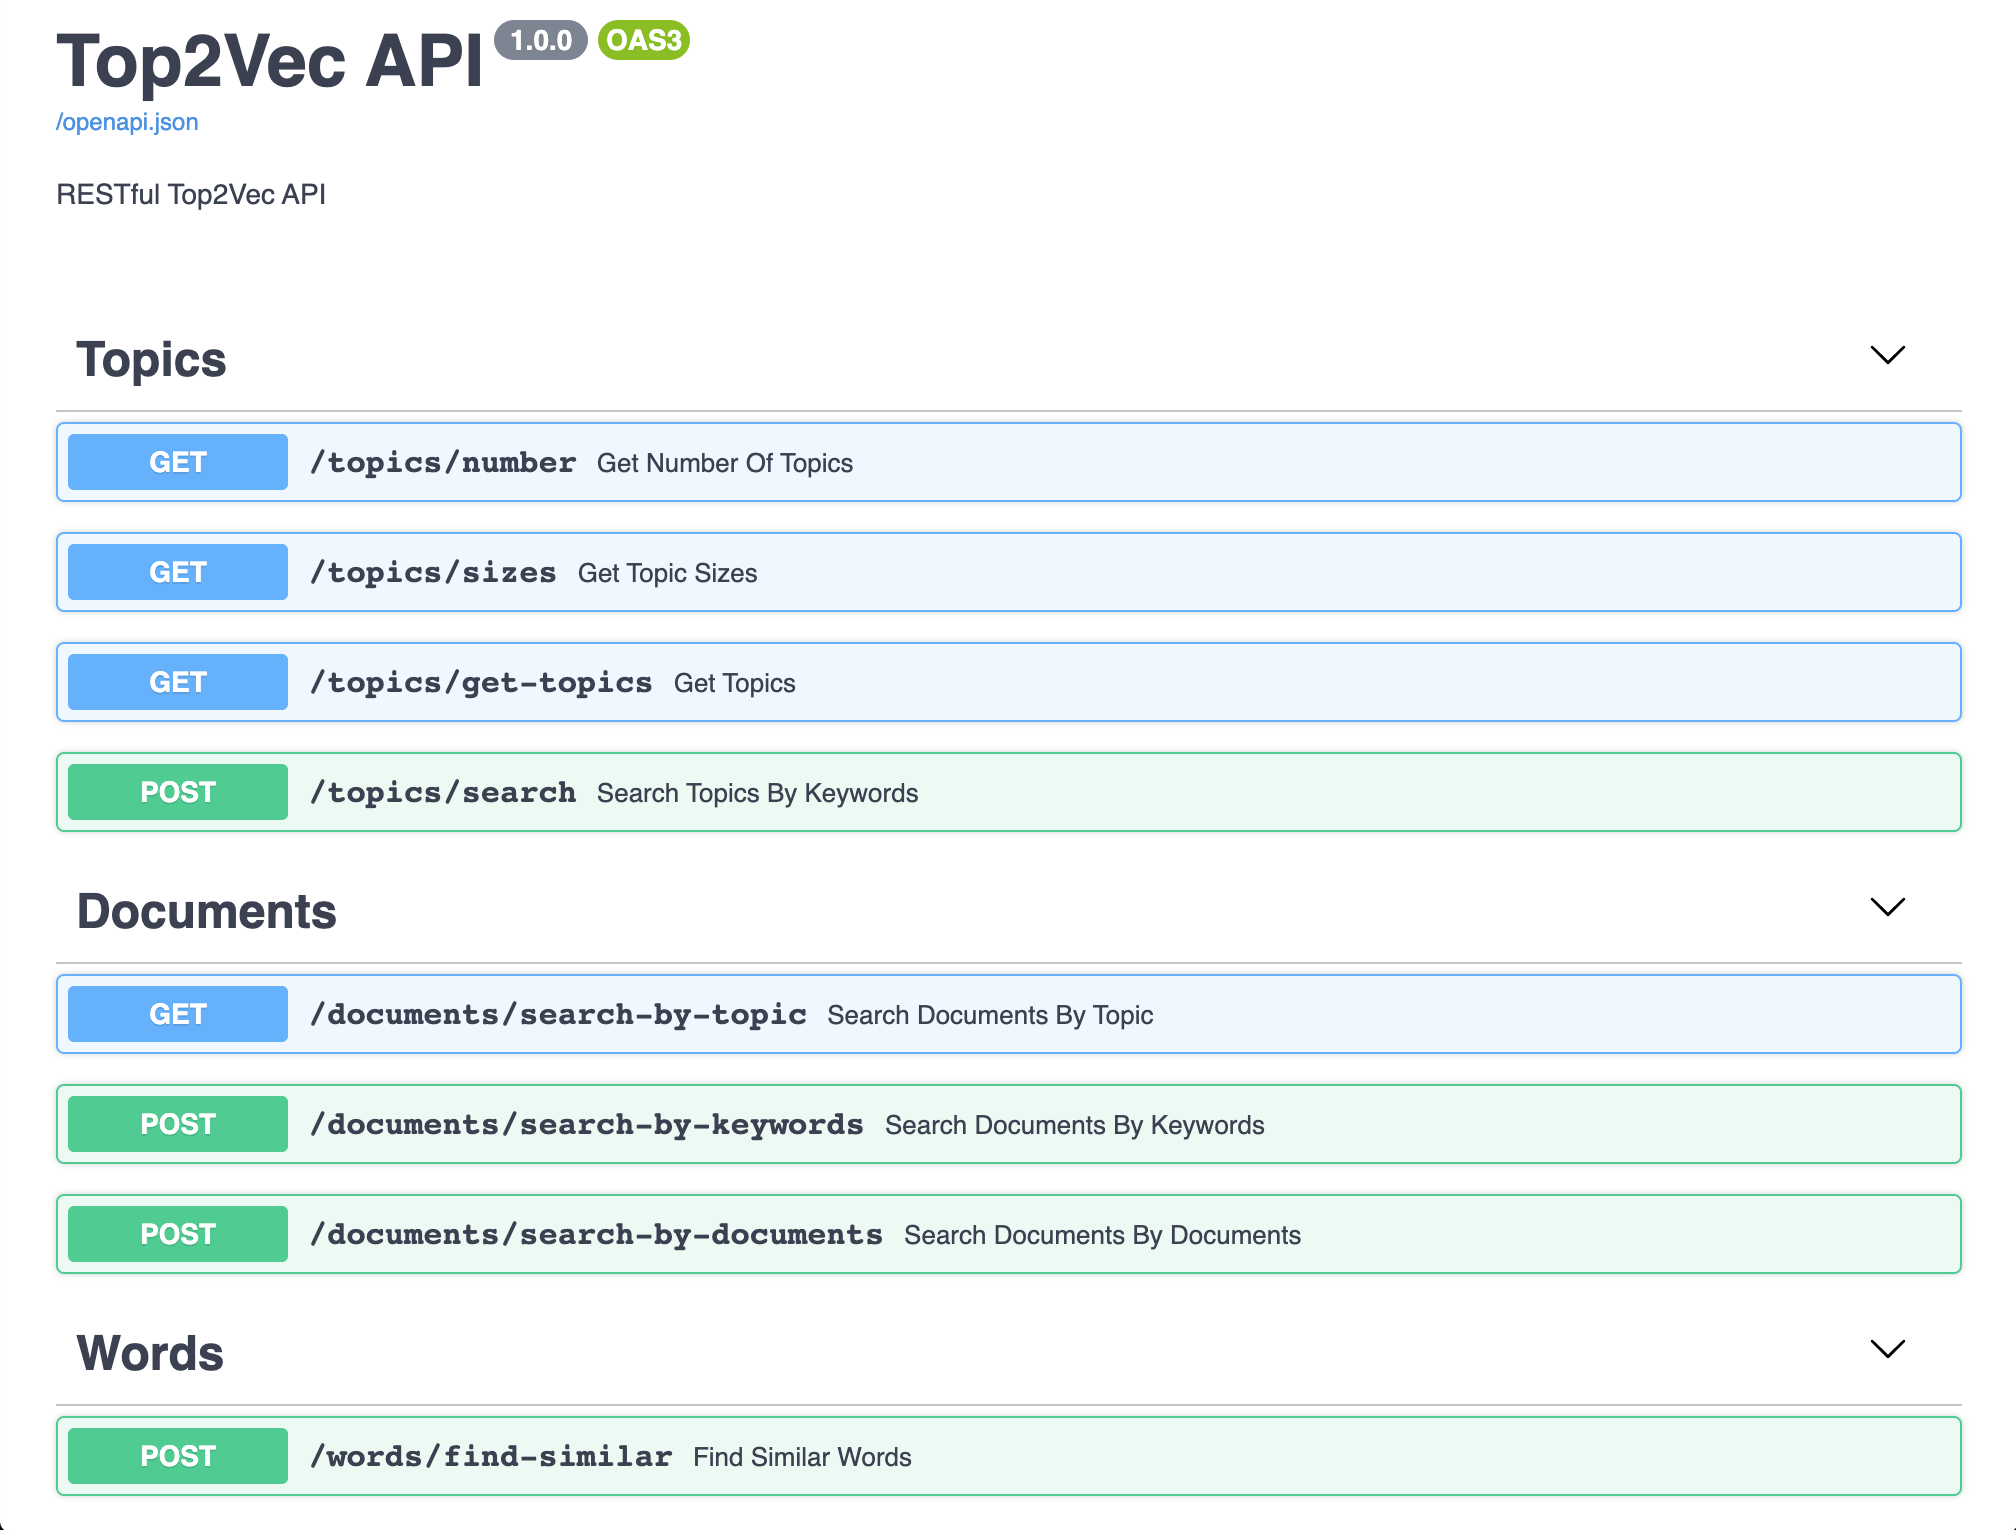
\includegraphics[width=12cm]{img/3.1.restful-top2vec.png}
    \caption{API proposé par Top2Vec}
    \label{fig:api_top2vec}
\end{figure}

\subsubsection{L'algorithme de Top2Vec}
Dans un premier temps, Top2Vec crée des vecteurs de documents et de mots intégrés conjointement à l'aide de Doc2Vec. L'image \ref{fig:docword} illustre un exemple dans lequel les documents qui sont placés à proximité des autres documents similaires et à proximité des mots les plus distinctifs.

\begin{figure}[H] %[!ht]
    \centering
    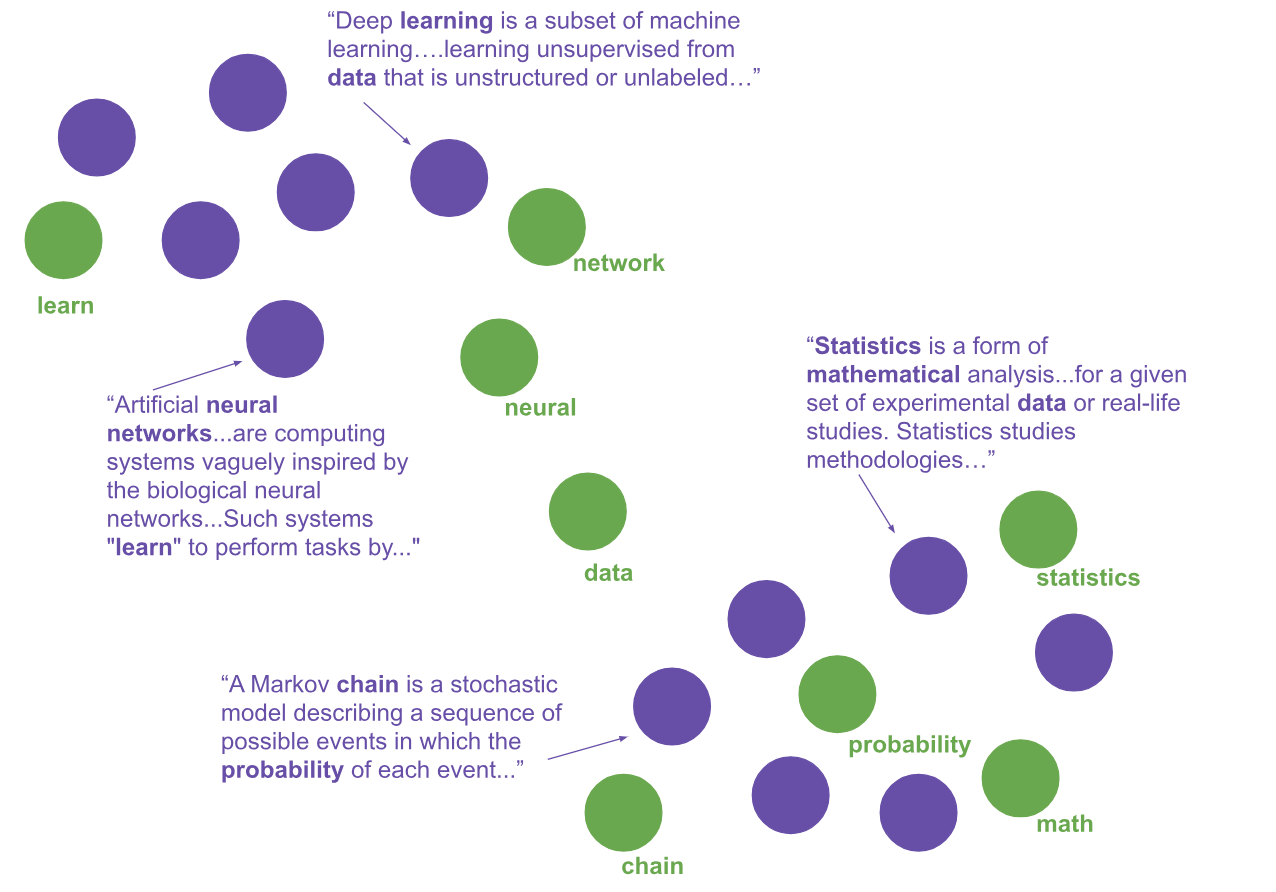
\includegraphics[width=12cm]{img/doc_word_embedding.png}
    \caption{L'emplacement des documents similaires dans l'espace des vecteurs}
    \label{fig:docword}
\end{figure}

Dans le NLP et l’apprentissage automatique, les documents sont souvent représentés sous forme de vecteurs de grande dimension. Chaque dimension de ces vecteurs peut correspondre à un terme (mot) unique dans un vocabulaire, ce qui donne des milliers, voire des millions de dimensions pour un seul document.
Les vecteurs de documents dans un tel espace de grande dimension sont très clairsemés, donc la deuxième étape dans le procès de formation est de réduire des dimensions, qui aide à trouver des zones denses. 
La réduction de dimensions de vecteurs de documents fait référence au processus de réduction des représentations vectorielles originales des documents tout en préservant leurs informations et caractéristiques essentielles.
Cette étape est montrée dans l'image \ref{fig:step2_top2vec}, avec chaque point est un vecteur de document. \footnote{Les images d'illustration de l'algorithme dans cette section sont de la source \cite{Ddangelov}}

\begin{figure}
     \centering
     \begin{subfigure}[b]{0.9\textwidth}
         \centering
         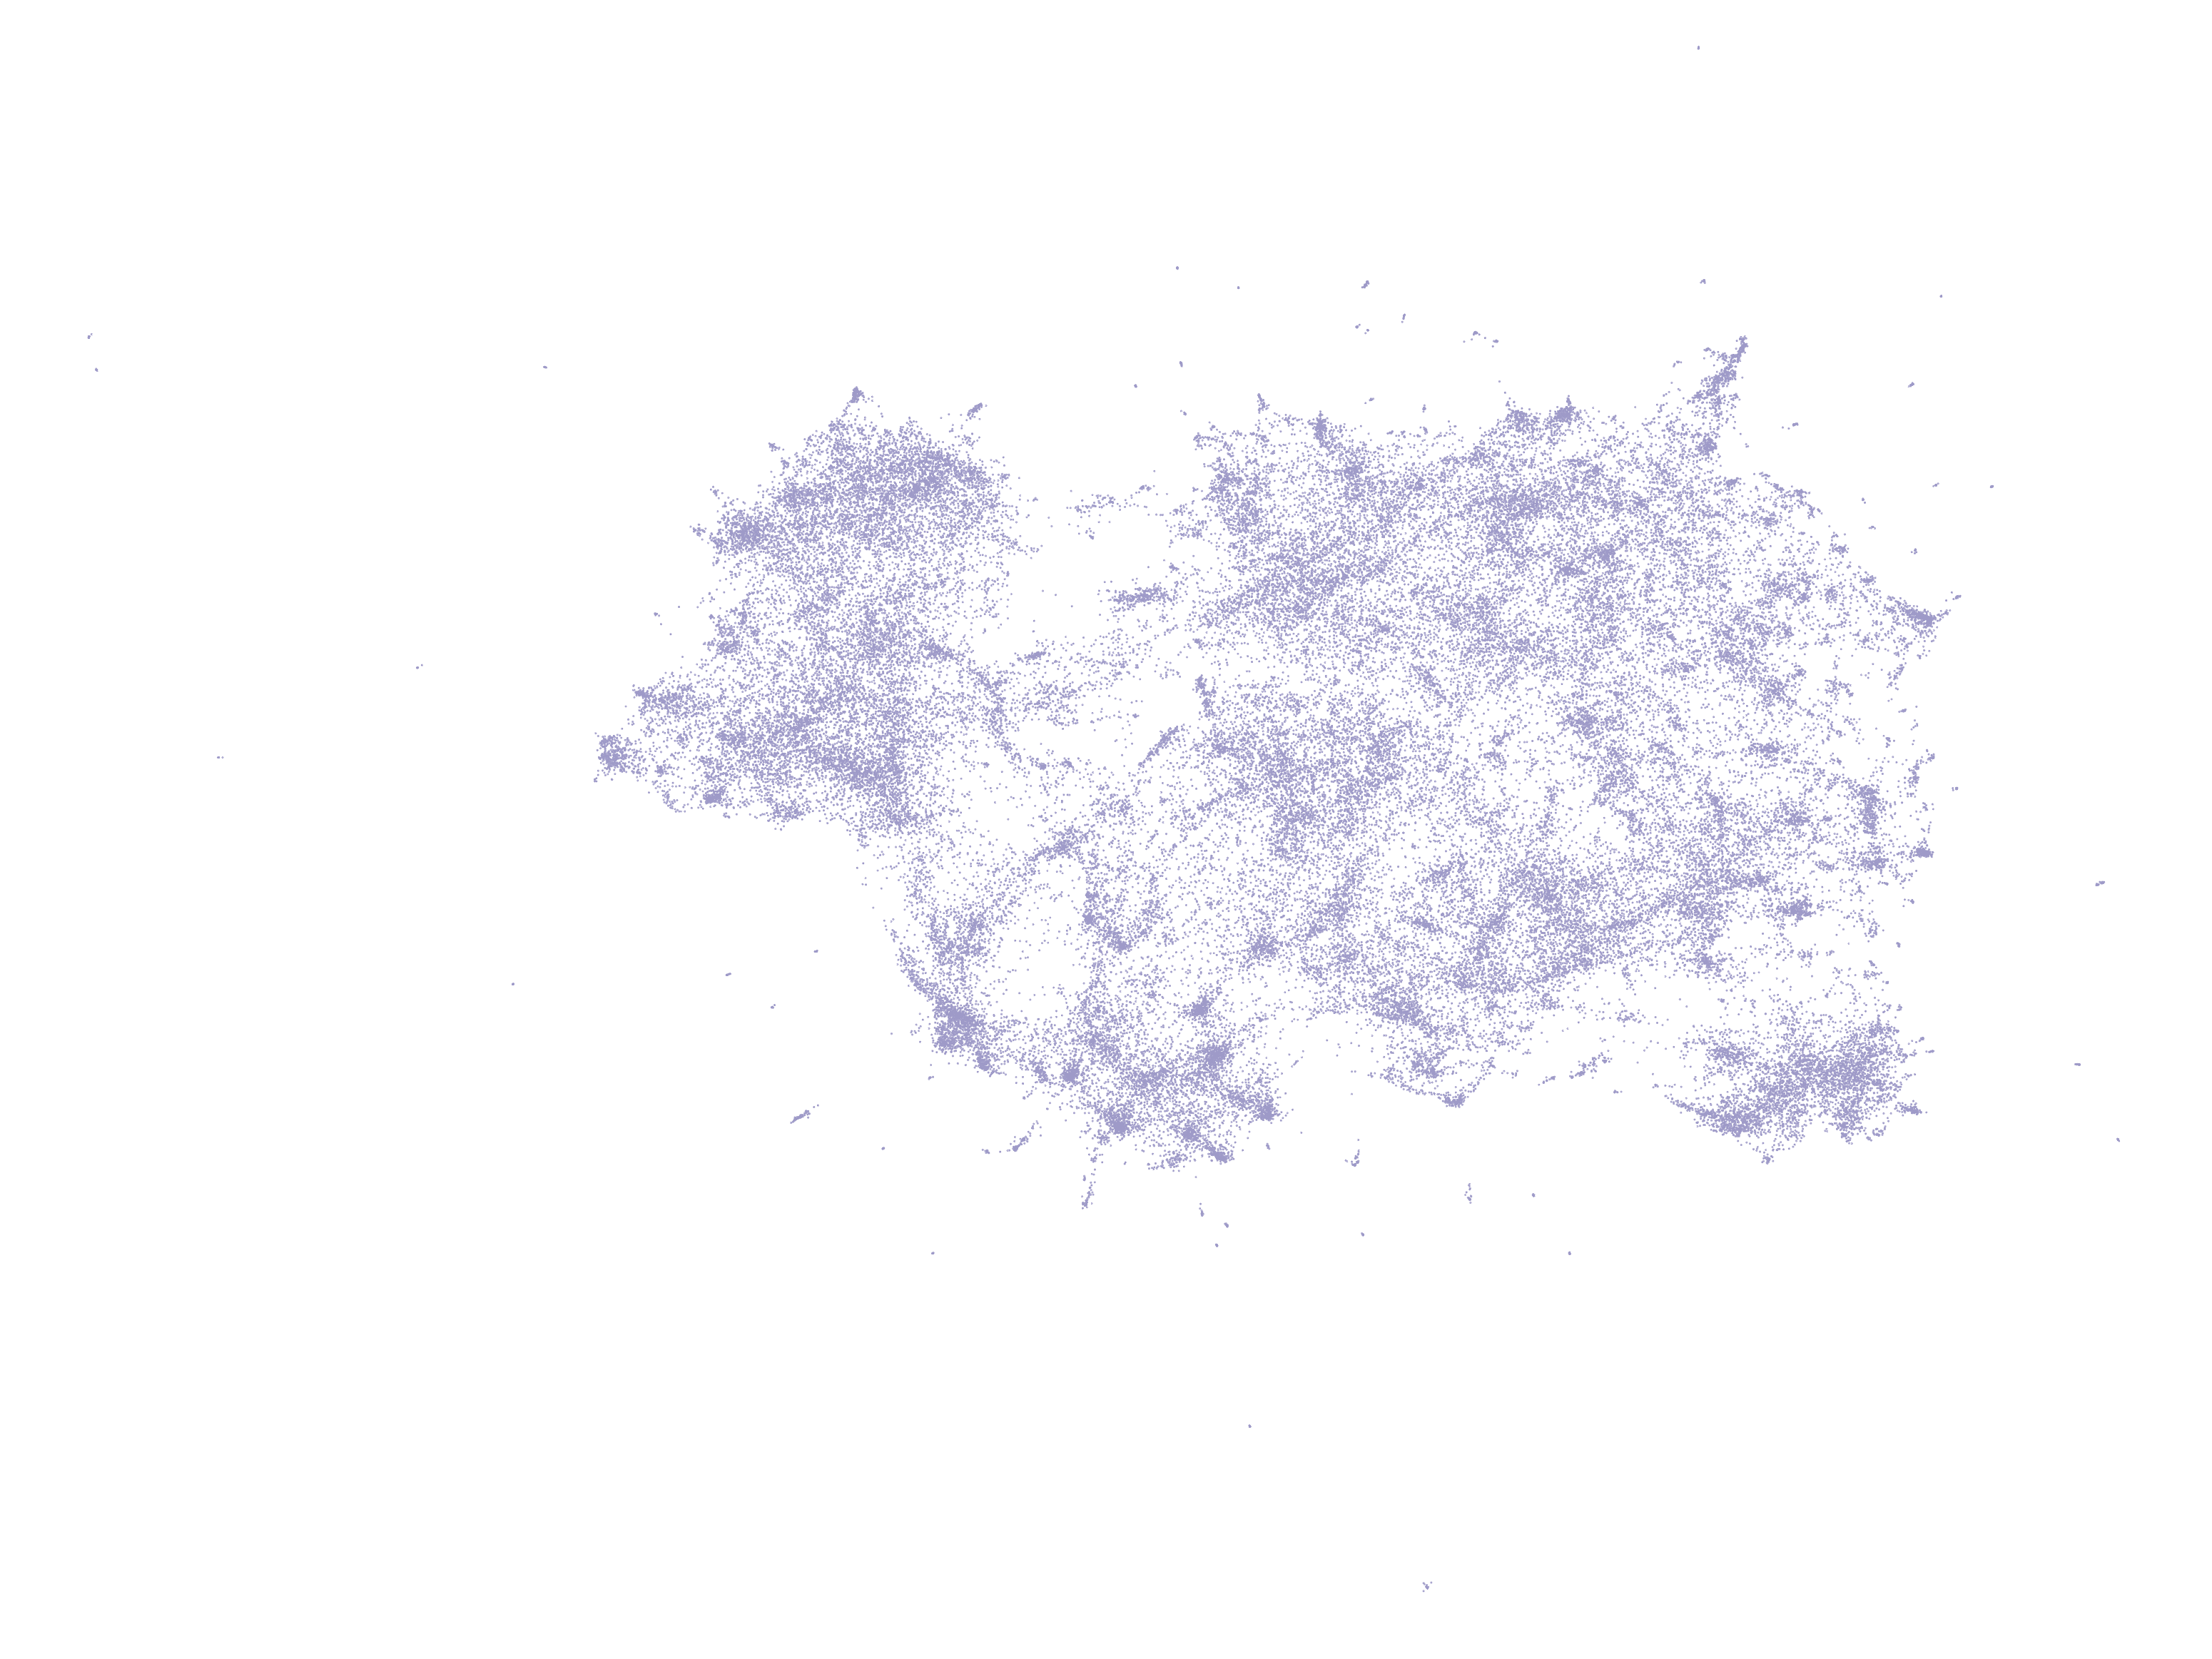
\includegraphics[width=\textwidth]{img/sparse.png}
         \caption{Les vecteurs de grande dimension}
         % \label{fig:tp12_0}
     \end{subfigure}
     \hfill
     \begin{subfigure}[b]{0.9\textwidth}
         \centering
         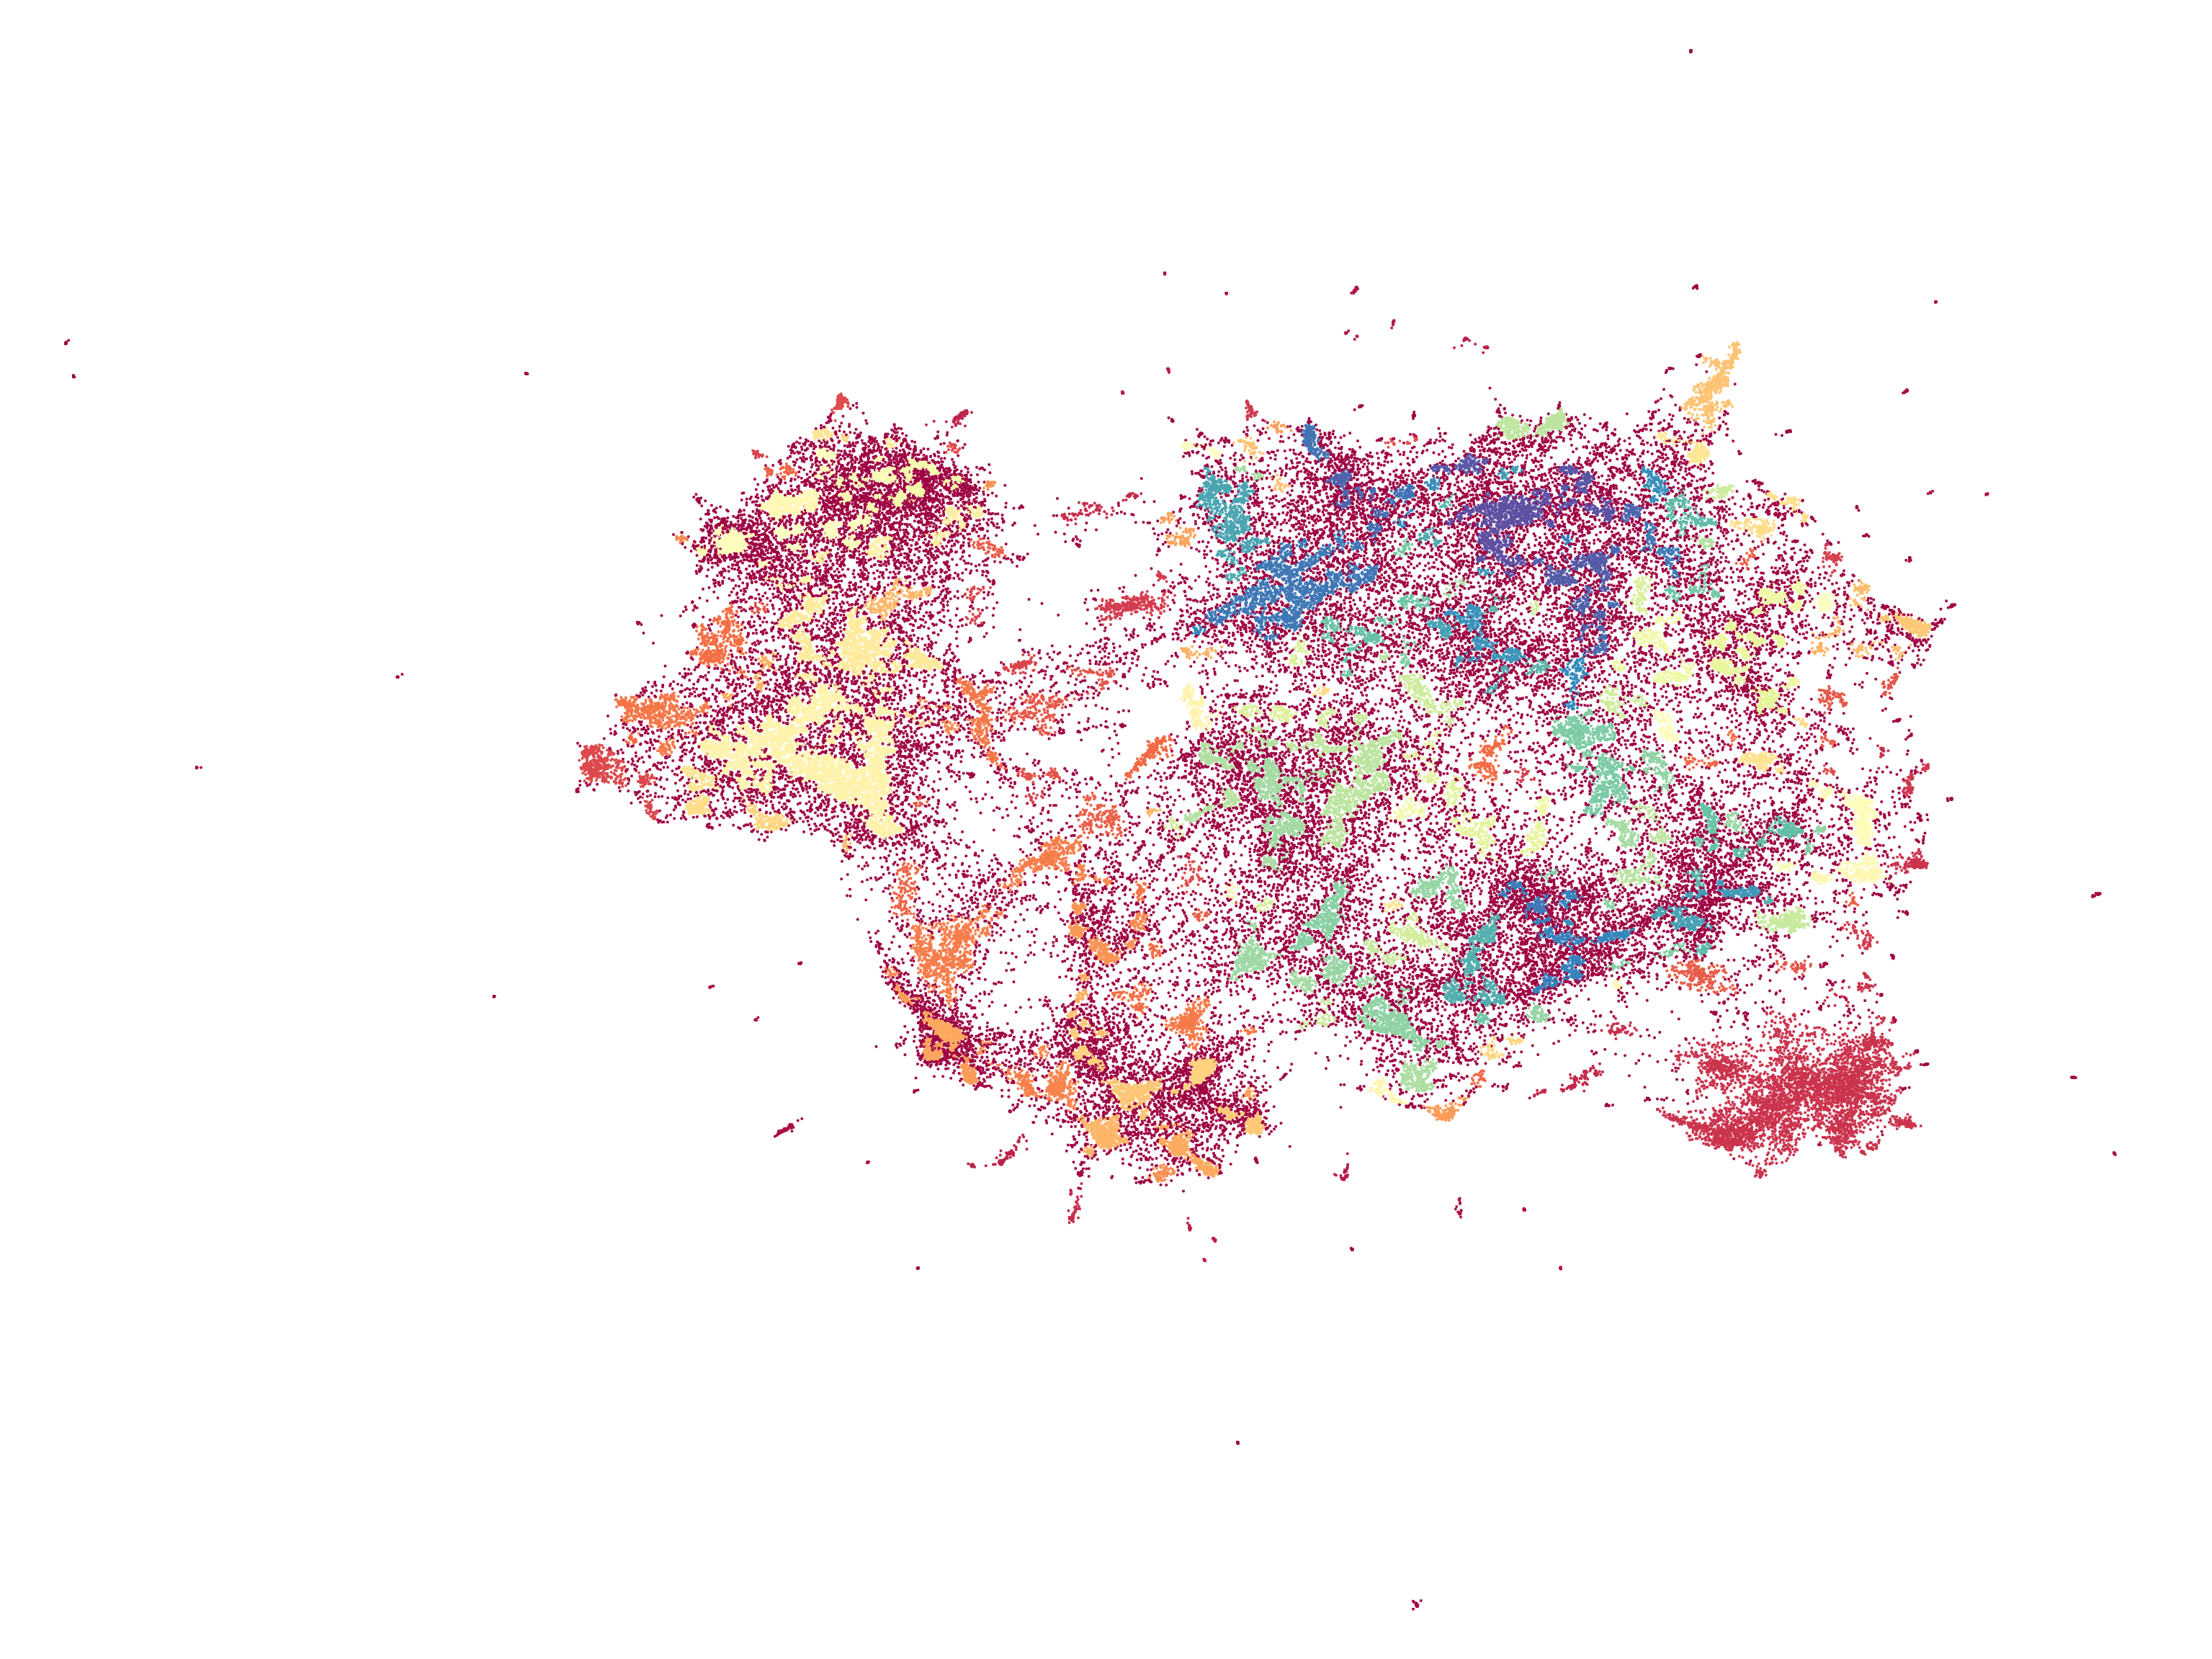
\includegraphics[width=\textwidth]{img/dense.png}
         \caption{Les zones denses des vecteurs de dimension réduite}
         % \label{fig:dense}
     \end{subfigure}
     \hfill
        \caption{La recherche des zones denses avec la réduction de dimension}
    \label{fig:step2_top2vec}
\end{figure}

Ensuite, Top2Vec calcule le centroïde des vecteurs de document pour chaque zone dense, ce centroïde est le vecteur du sujet.
Dans la figure \ref{fig:topic_vector}, les points rouges sont des documents aberrants et ne sont pas utilisés pour calculer le vecteur thématique. Les points violets sont les vecteurs de documents appartenant à une zone dense, à partir de laquelle le vecteur thématique est calculé.

\begin{figure}[H] %[!ht]
    \centering
    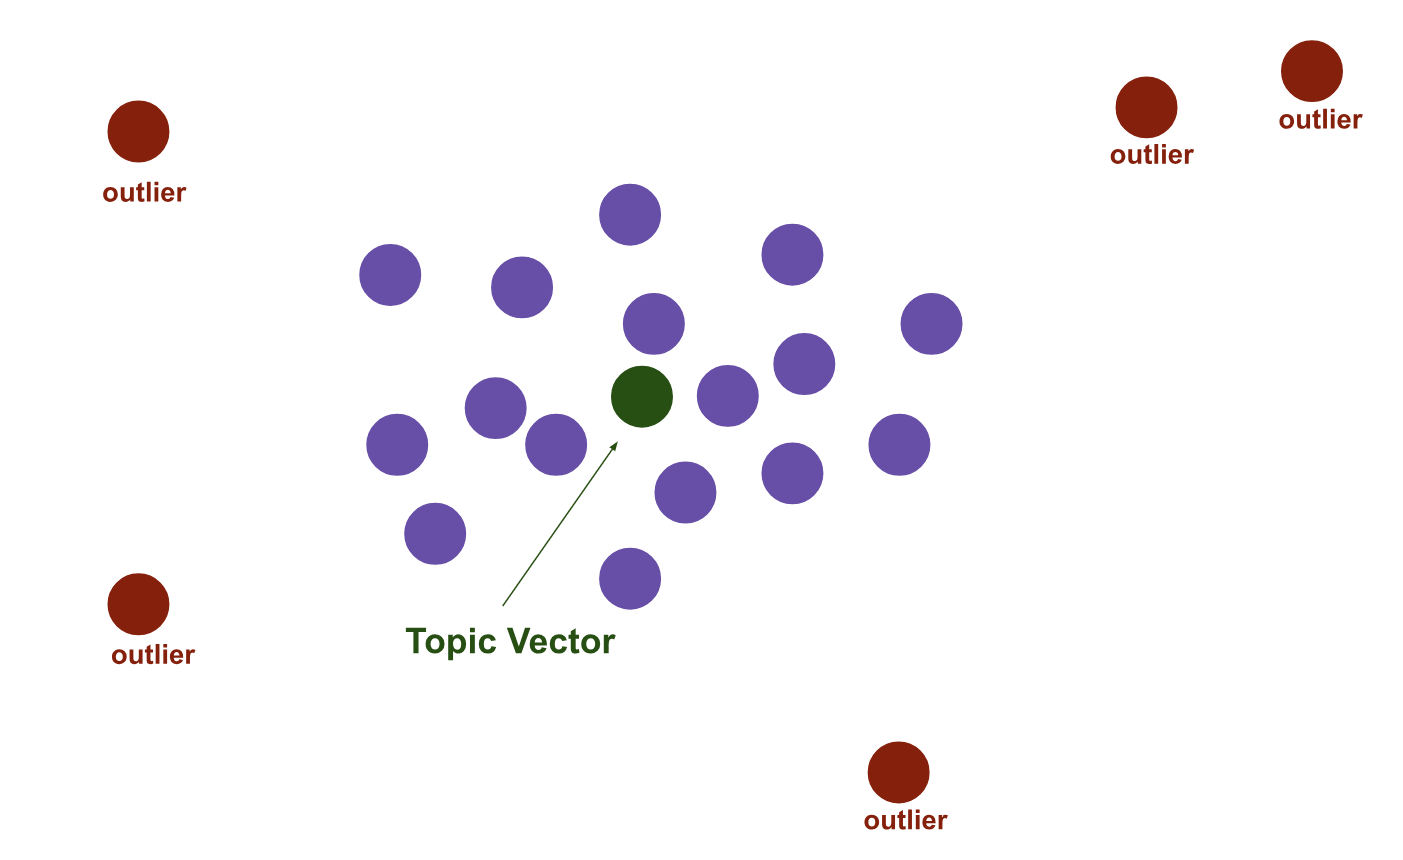
\includegraphics[width=12cm]{img/topic_vector.png}
    \caption{Calcul du centroïde de zone dense alias vecteur du sujet}
    \label{fig:topic_vector}
\end{figure}

Finalement, les vecteurs de mots les plus proches dans la figure \ref{fig:find_keyword} par ordre de proximité deviennent les mots thématiques. Dans Top2Vec, la recherche des plus proches voisins (N-Nearest) est utilisée pour trouver les mots-clés du sujet. 

\begin{figure}[H] %[!ht]
    \centering
    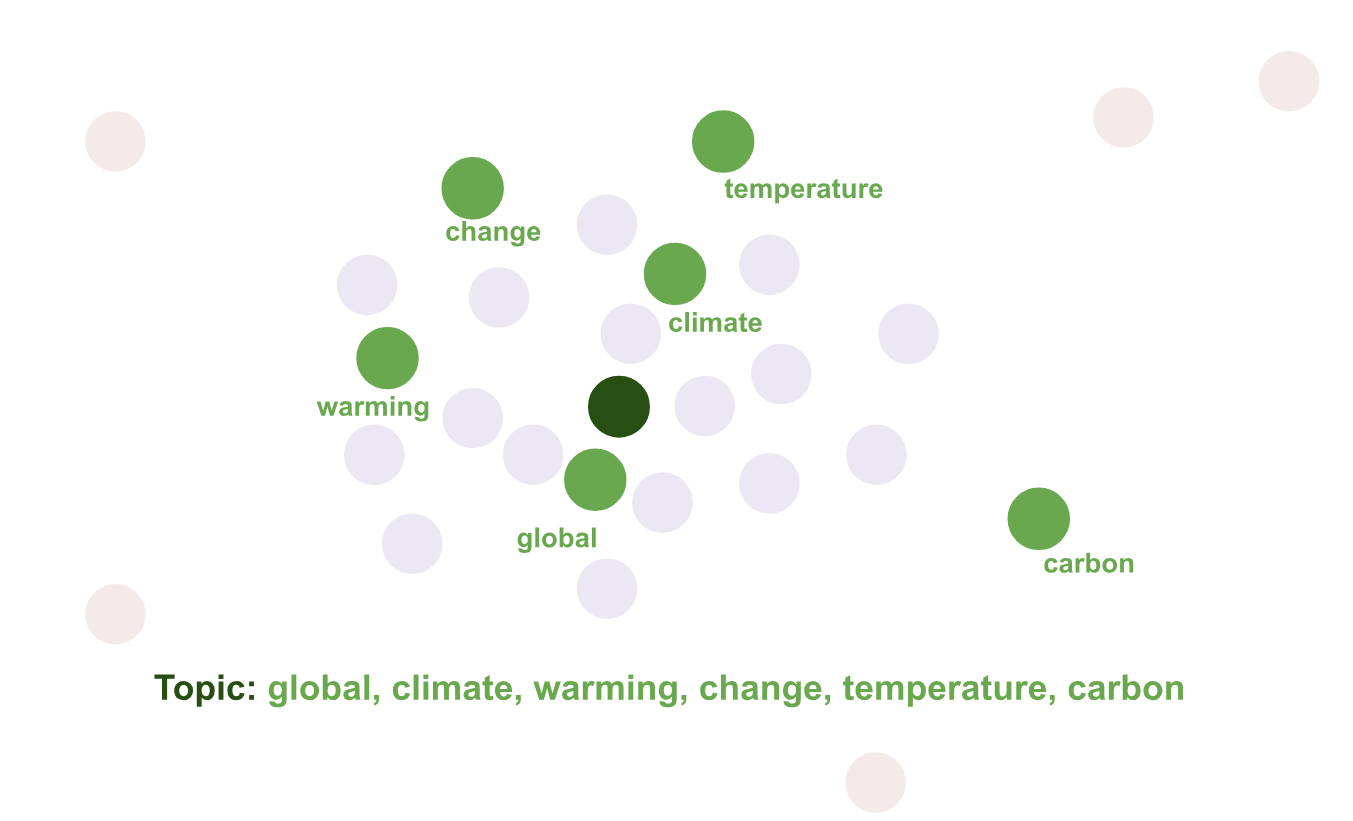
\includegraphics[width=12cm]{img/find_keyword.png}
    \caption{Recherche de mots clés qui sont les mots plus proches au centroïde}
    \label{fig:find_keyword}
\end{figure}

\subsubsection{Structure de l'implémentation}
\textbf{L'objectif de cette étude} est d'effectuer une classification optimale des thèmes présents dans le corpus, en mettant particulièrement l'accent sur les documents de recherche et scientifiques de l'époque de l'Indochine.

Dans la première phase, nous procéderons à plusieurs entraînements en utilisant les modèles LDA et Top2Vec. L'objectif est de comparer l'efficacité de ces deux méthodes. Les résultats devraient confirmer la supériorité de Top2Vec sur LDA en ce qui concerne la modélisation thématique de notre corpus. Nous examinerons également l'impact de certains paramètres essentiels du modèle, notamment le paramètre \textit{min\_count}, qui détermine la fréquence minimale requise pour qu'un mot soit pris en considération, et le paramètre \textit{ngram\_vocab}, qui permet de choisir entre l'analyse de mots individuels ou de collocations n-grammes dans le corpus.

Dans la deuxième phase, nous entreprendrons des ajustements sur le corpus en réduisant certaines catégories de documents moins pertinentes et moins contributives à la thématique scientifique que nous souhaitons identifier. Les résultats de cette étape confirment notre hypothèse selon laquelle le modèle Top2Vec présente encore certaines limites, car il ne parvient pas à détecter les sous-thèmes latents au sein des grands thèmes.

En utilisant un modèle Word2Vec, nous introduisons une étape supplémentaire dans notre processus de modélisation thématique pour les sous-thèmes latents. Nous utilisons des ensembles de mots-clés générés par un modèle Word2Vec bien entraîné, qui prend en compte les mots de faible fréquence dans les documents. Parallèlement, un nouveau modèle Top2Vec est également entraîné en utilisant la même fréquence d'occurrence. Cette approche nous permet d'obtenir des modèles plus compétents dans la compréhension des mots, ce qui facilite la détection précise de petits sous-thèmes associés à des mots-clés spécifiques.

\subsection{Une comparaison de modélisation des sujets entre LDA et Top2Vec}
\subsubsection{LDA performance}
Pour effectuer une allocation de Dirichlet latente (LDA) sur notre corpus, nous utilisons la bibliothèque Gensim. Dans le code ci-dessous, nous créons un dictionnaire Gensim et une représentation de corpus en sac de mots (BoW) à partir du texte prétraité. Ensuite, nous construisons un modèle LDA avec num\_topics = 5 qui définit le nombre de sujets à étudier arbitrairement.

\begin{lstlisting}
# Create a dictionary and a corpus from the preprocessed text
dictionary = corpora.Dictionary(filtered_corpus)
corpus_bow = [dictionary.doc2bow(doc) for doc in filtered_corpus]
# Build the LDA model
lda_model = LdaModel(corpus_bow, num_topics=5, id2word=dictionary, passes=15)
\end{lstlisting}

A la fin de la formation, nous obtenons 5 sujets avec les mots-clés suivants :\newline
\textit{Topic 0: faire,grand,bien,roi,pays,jour,travail,français,cochinchine,chinois \newline
Topic 1: vietnamien,nam,chinois,nguy,langue,étude,thi,bien,histoire,grand\newline
Topic 2: grand,faire,bien,homme,jour,nom,petit,année,chinois,long\newline
Topic 3: société,membre,comité,président,séance,général,saigon,bulletin,etude,secrétaire\newline
Topic 4: saigon,faire,annamite,cochinchine,amiral,lettre,france,pari,bien,français}

Dès la première impression, il est difficile de tirer le thème de chaque sujet en regardant ces mots-clés. Nous essaierons d'extraire quelques documents qui présentent une meilleure similitude dans chaque sujet. Par exemple dans le sujet 0, nous avons trouvé une classe de documents autour du thème de l'architecture ou des monuments de l'époque :\newline
\textit{Document 2 (1799 mots) - Similarité : 1.00 - vue ensemble sculpture modelage chine durant vingt siècles\newline
  Document 3 (11273 mots) - Similarité : 1.00 - vérification dates inscriptions monuments khmers seconde partie\newline
  Document 5 (1501 mots) - Similarité : 0.94 - etude monuments représentatifs art français saigon\newline
}

Mais aussi des documents des chansons :\newline
  \textit{Document 70 (16501 mots) - Similarité : 1.00 - chants antiques montagne\newline
  Document 71 (469 mots) - Similarité : 0.97 - chants populaires proverbes annamites\newline
  Document 114 (1966 mots) - Similarité : 0.98 - folklore musical jara bahnar}

Et les trois grand traductions du roman Les Trois Royaumes qui est le premier des Quatre livres extraordinaires de la littérature classique chinoise :\newline
\textit{Document 190 (73211 mots) - Similarité : 1.00 - trois royaumes traduction notes commentaires nghiêm to louis ricaud\newline
  Document 191 (32268 mots) - Similarité : 1.00 - trois royaumes traduction notes commentaires nghiêm to louis ricaud\newline
  Document 192 (66806 mots) - Similarité : 1.00 - trois royaumes traduction notes commentaires nghiêm to louis ricaud}

Nous constatons une incohérence entre les sujets des documents, qui s'explique principalement par le fait que la méthode LDA est basée sur un ensemble de mots fréquemment associés à ce sujet et pas sur leur relation thématique. LDA nécessite la spécification de paramètres, tels que le nombre de sujets (num\_topics). Si ces paramètres ne sont pas choisis de manière appropriée pour le corpus, les sujets résultants risquent de ne pas être significatifs. Le réglage de ces paramètres peut être difficile et nécessite souvent une expertise du domaine.
Dans ce travail, plusieurs tentatives sur différents paramètres ont été faites mais aucune ne propose une modélisation significative.
\footnote{Les résultats de deux autres modèles de 12 sujets et 24 sujets sont inclus en annexe de cette memoire.}

\subsubsection{Top2Vec performance}
La formation du Top2Vec est implémentée comme suit :
\begin{lstlisting}
from top2vec import Top2Vec
import multiprocessing
# Initialize Top2Vec model
model_T2V = Top2Vec(documents=preprocessed_corpus, 
                tokenizer=lambda x: x.split(), 
                min_count=200,
                speed='deep-learn',
                workers=(multiprocessing.cpu_count())
               )
\end{lstlisting}
Dans cet appel, le paramètre 'min\_count' représente la fréquence minimale à laquelle chaque mot doit apparaître dans le corpus pour être pris en compte. Par exemple, min\_count=100 exige que chaque mot soit présent au moins 100 fois dans le corpus pour être inclus dans le modèle. Le paramètre 'speed' détermine la vitesse à laquelle le modèle est entraîné. L'option 'fast-learn' est la plus rapide mais génère des vecteurs de moindre qualité. L'option 'learn' génère des vecteurs de meilleure qualité mais prend plus de temps à s'entraîner. L'option 'deep-learn' apprend les vecteurs de la meilleure qualité mais nécessite beaucoup plus de temps d'entraînement. Comme l'option 'deep-learn' est choisie, le nombre maximal de threads de travail (workers) est utilisé pour accélérer la formation du modèle.

Nous présentons ici un modèle entraîné avec les mots apparaissant au moins 200 fois. Après l'apprentissage automatique, Top2Vec retourne un regroupement de 10 sujets avec les mots-clés suivants :

\begin{tabular}{|p{15cm}|}
\hline
Regroupement des sujets et les mot-clés\\
\hline
\textbf{Sujet} \textbf{1 }:  lecteur,  pensée,  savant,  étudier,  historien,  civilisation  scientifique,  intellectuel,  auteur,  ouvrage \\ \hline
\textbf{Sujet} \textbf{2} :  surface,  liquide,  sec,  couche,  mètre,  diamètre,  épaisseur,  sol , profondeur,  tige\\ \hline
\textbf{Sujet} \textbf{3} : comité,  membre,  bulletin,  secrétaire,  président,  séance,  réunion  assemblée,  publication,  commission \\ \hline
\textbf{Sujet} \textbf{4} :  amiral,  navire,  capitaine,  expédition,  commandant,  marine  gouvernement,  armer,  établissement,  port \\ \hline
\textbf{Sujet} \textbf{5} : génie,  offrande,  prière,  buffle,  divinité,  parent,  autel  laotien,  maison,  sacrifice \\ \hline
\textbf{Sujet} \textbf{6} :  monument,  angkor,  relief,  sculpture,  édifice,  temple,  style  statue,  khmèr,  décor \\ \hline
\textbf{Sujet} \textbf{7} :  nên,  làm,  nào,  qua,  cœur,  cho,  khi,  mari,  aimer,  nhà  \\ \hline
\textbf{Sujet} \textbf{8} :  asia,  studie,  vietnam,  asie,  rét,  thai,  tnam,  viet,  van,  nam \\ \hline
\textbf{Sujet} \textbf{9} :  géographie,  agriculture,  société,  annal,  journal,  revue,  agricole  colonial,  indo,  tonkin \\ \hline
\textbf{Sujet} \textbf{10} :  directeur,  professeur,  secrétaire,  rue,  président,  administrateur  général,  collège,  colonial,  municipal \\ 
\hline
\end{tabular}
\vspace{1cm}

Intuitivement, les mots-clés de chaque sujet se présentent de manière plus cohérente autour d'un thème spécifique, ce qui nous permet de nommer directement chaque sujet. Par exemple, le thème 1 couvre des mots liés à l'agriculture et aux plantations, le thème 3 s'agit des documents militaires, et le thème 5 mentionne l'architecture et les monuments d'Angkor-Vat (Cambodge). Voici une liste de documents faisant partie des documents les plus similaires dans le sujet "Agriculture" :
\begin{itemize}
    \item culture de l \textbf{abaca} lettre de m le gérant du consulat général de manille 1889
    \item courtes notices sur l indochine i l opium ii les \textbf{pêcheries} la \textbf{préparation} du nuoc mam les salines 1898
    \item rapport présenté par m j josselme sur la culture du \textbf{rocou} 1883 
    \item rapport sur la culture du \textbf{jute} 1895 
    \item de la préparation en cochinchine des \textbf{fromages} de pate de \textbf{haricots} \item notice sur la culture du \textbf{café} libéria 1888
    \item remarques faites dans le drainage d une \textbf{tourbière bois} de trams et armes ou outils en pierre taillée dans la \textbf{tourbe} 1884 
    \item mémoire sur le \textbf{sulfatage} des \textbf{céréales} 1883
    \item notice sur le mac lua \textbf{plante} \textbf{tinctoriale} 1887 
\end{itemize}


On peut observer dans la figure \ref{fig:heatmap} les cartes thermiques (heatmap) qui visualisent les scores de similarité entre 4 modèles en faisant varier les valeurs de min\_count entre 50, 100, 200 et 400. De manière générale, on constate une faible similarité entre les différents sujets. Le modèle avec une fréquence d'occurrence des mots comprise entre 100 et 200 génère plus de sujets que les modèles avec un min\_count de 50 ou 400, ce qui confirme notre hypothèse selon laquelle il existe une plage de fréquence à laquelle les mots deviennent plus bruyants (faible/moyenne fréquence, par exemple 50) ou plus génériques (haute fréquence, par exemple 400). En ce qui concerne la similarité, le modèle à 100 fréquences présente les meilleurs résultats, car il comporte moins de sujets fortement similaires que le modèle à 200 fréquences, par exemple les sujets 7, 8 et 9.

\begin{figure}[H]
        \centering
        \begin{subfigure}[b]{0.45\textwidth}
            \centering
            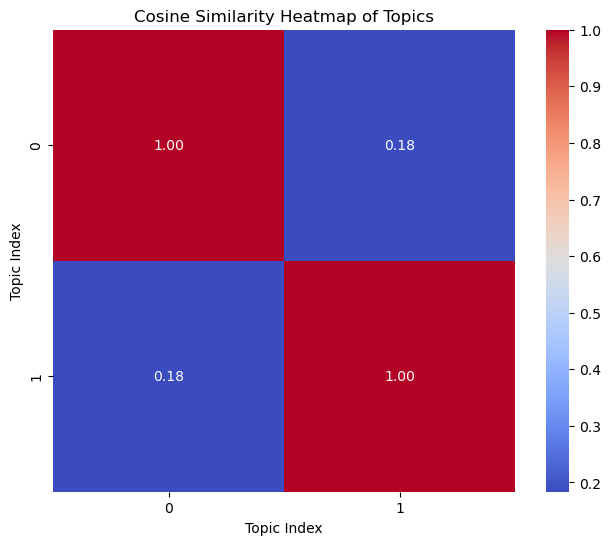
\includegraphics[width=\textwidth]{img/3.2acosine_sim_50_ngram_deep.png}
            \caption[min\_count = 50]%
            {{\small min\_count = 50}}    
            % \label{fig:50}
        \end{subfigure}
        \hfill
        \begin{subfigure}[b]{0.45\textwidth}  
            \centering 
            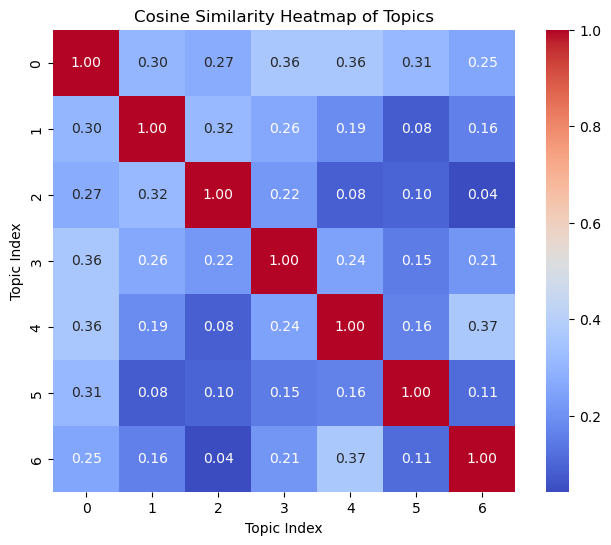
\includegraphics[width=\textwidth]{img/3.2bcosine_sim_100_ngram_deep.png}
            \caption[min\_count = 100]%
            {{\small min\_count = 100}}    
            % \label{fig:100}
        \end{subfigure}
        \vskip\baselineskip
        \begin{subfigure}[b]{0.45\textwidth}   
            \centering 
            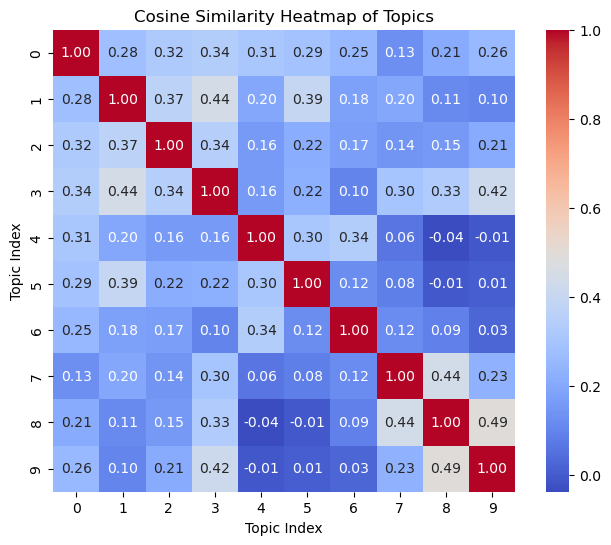
\includegraphics[width=\textwidth]{img/3.2ccosine_sim_200_ngram_deep.png}
            \caption[min\_count = 200]%
            {{\small min\_count = 200}}    
            % \label{fig:200}
        \end{subfigure}
        \hfill
        \begin{subfigure}[b]{0.45\textwidth}   
            \centering 
            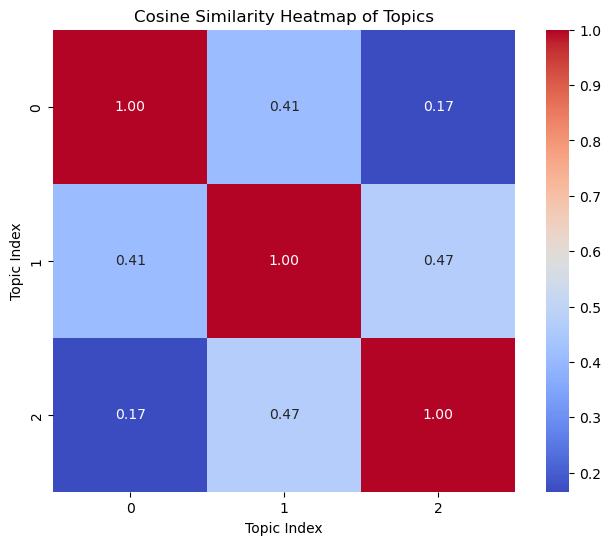
\includegraphics[width=\textwidth]{img/3.2d.cosine_sim_400_ngram_deep.png}
            \caption[min\_count = 400]%
            {{min\_count = 400}}    
            % \label{fig:400}
        \end{subfigure}
        \caption {Carte thermique de la similarité du modèle utilisant différentes valeurs min\_count}
        \label{fig:heatmap}
    \end{figure}

\subsubsection{Entraînement  des sujets avec les collocations ngram}
Non seulement il regroupe les documents en fonction de l'entraînement des mots individuels, mais Top2Vec est également capable de détecter les expressions courantes dans le corpus et de les ajouter au vocabulaire des sujets.

En utilisant le paramètre \textit{ngram\_vocab = True}, le modèle s'entraîne  pour repérer les collocations fréquentes et les considérera lors de la classification des sujets, ce qui renforcera davantage l'identité de chaque sujet par rapport aux mots individuels.

\begin{lstlisting}
mincount = 200
train_speed = 'deep-learn'
model_test_param = Top2Vec(documents=preprocessed_corpus, 
            tokenizer=lambda x: x.split(), 
            min_count=mincount,
                ngram_vocab = True,
            speed=train_speed,
            workers=(multiprocessing.cpu_count() )
           )
model_test_param.save(f'model_ngram_{mincount}_{train_speed}')
\end{lstlisting}

La Figure \ref{wc_militaire_2gram} présente le nuage de mots générés pour le sujet militaire, qui inclut des bigrammes tels que "expédition militaire", "armée canon", "capitaine vaisseau", "port Touraine".

\begin{figure}[H] %[!ht]
    \centering
    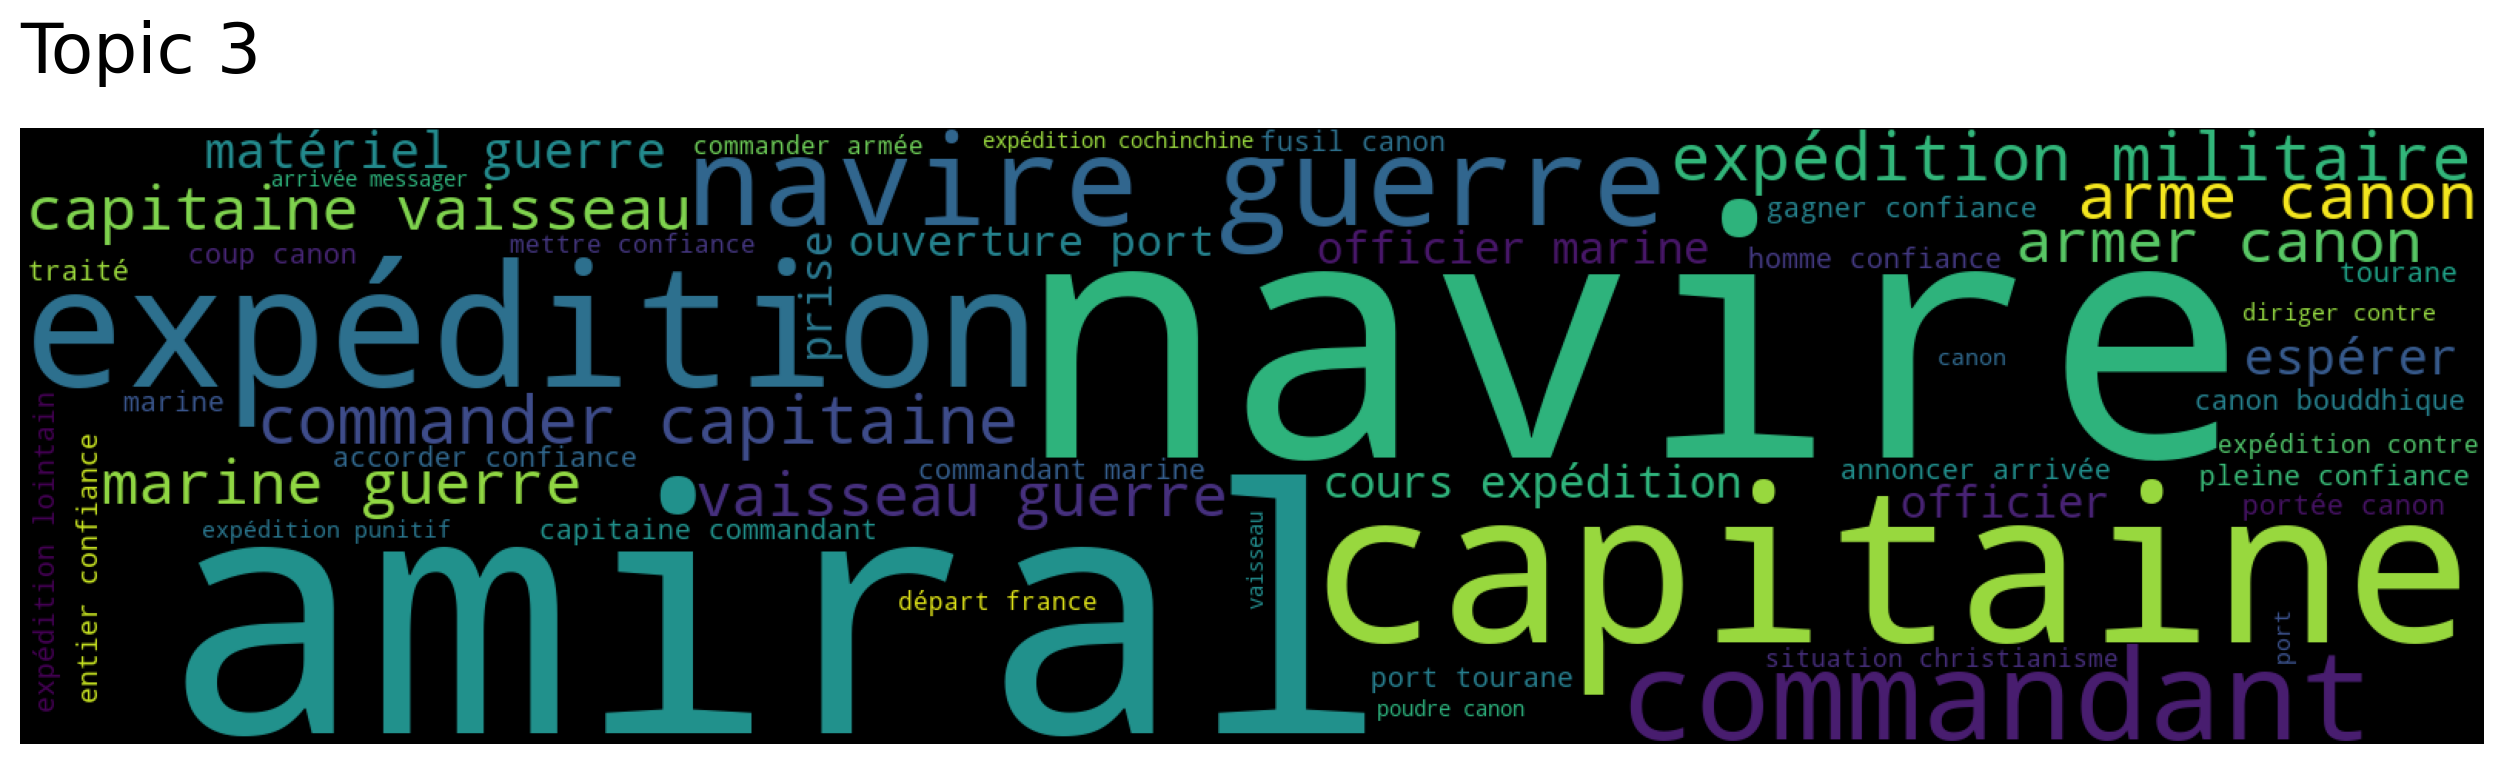
\includegraphics[width=14cm]{img/3.4.wc_militaire.png}
    \caption{WordCloud du sujet militaire avec un modèle de ngram\_vocab}
    \label{wc_militaire_2gram}
\end{figure}

\subsection{Analyses des significations des sujets}

La Figure \ref{fig:topic_size_docs} illustre la distribution de documents parmi les sujets regroupés, y compris ceux que nous avons considérés comme peu utiles, obtenus à la suite d'un entraînement avec l'option ngram\_vocab. Nous pouvons observer que trois grands sujets, à savoir "recherche générale", "militaire" et "traduction/bilingue en vietnamien", représentent une grande partie du corpus, tandis que les groupes de documents 7, 9 et 10 contiennent très peu de documents. Un autre groupe que nous avons identifié  comme "divers" - groupe 4 par contre inclut beaucoup de documents, avec les autres sujets tels que "agriculture", "architecture", "ethnies du Laos", "études asiatiques" et "traduction/bilingue en chinois", chacun de ces sujets occupe également une part importante du corpus. Nous allons examiner de plus près le contenu de chaque groupe de documents afin de mieux comprendre leur vraie signification. Nous espérons identifier les avantages et les inconvénients de cette méthode de regroupement.

\begin{figure}[H] %[!ht]
    \centering
    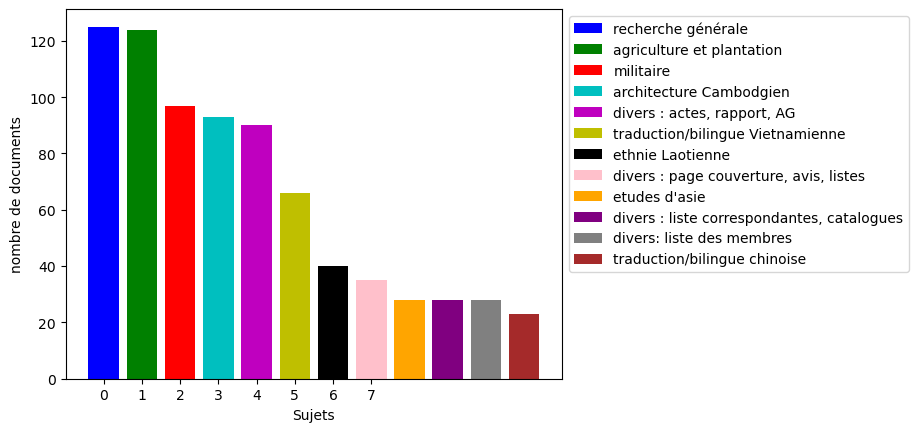
\includegraphics[width=14cm]{img/topic_size_docs.png}
    \caption{Répartition du nombre de documents entre les sujets regroupés}
    \label{fig:topic_size_docs}
\end{figure}

En plus du sujet militaire que nous avons examiné en détail avec son nuage de mots dans la section précédente (voir Figure \ref{wc_militaire_2gram}), notre analyse a également identifié d'autres sujets populaires dans le corpus qui sont détectés de manière assez précise. Parmi ces sujets figurent "Agriculture et Plantation" ainsi que "Recherche générale," qui comprend principalement des documents de recherche en histoire et en sciences humaines. Les nuages de mots correspondants sont visibles dans les Figure \ref{fig:tp12_0} et \ref{fig:tp12_1}.

Cependant, l'inconvénient de ces sujets est qu'ils semblent être un peu trop généraux en ce qui concerne les thèmes qu'ils englobent. Cela suggère qu'il existe encore davantage de sujets intéressants qui se cachent sous chaque thème principal. Par exemple, dans le sujet 1 - "Agriculture et Plantation," il est possible de trouver des articles portant sur des sujets tels que la médecine et les maladies, la nourriture ou la cuisine de l'époque. De même, dans le sujet 0 - "Recherche historique et humanités," les sujets de recherche demeurent trop vastes et peuvent englober d'autres thèmes plus spécifiques à l'intérieur de leur champ d'étude.

\begin{figure}[H]
     \centering
     \begin{subfigure}[b]{0.9\textwidth}
         \centering
         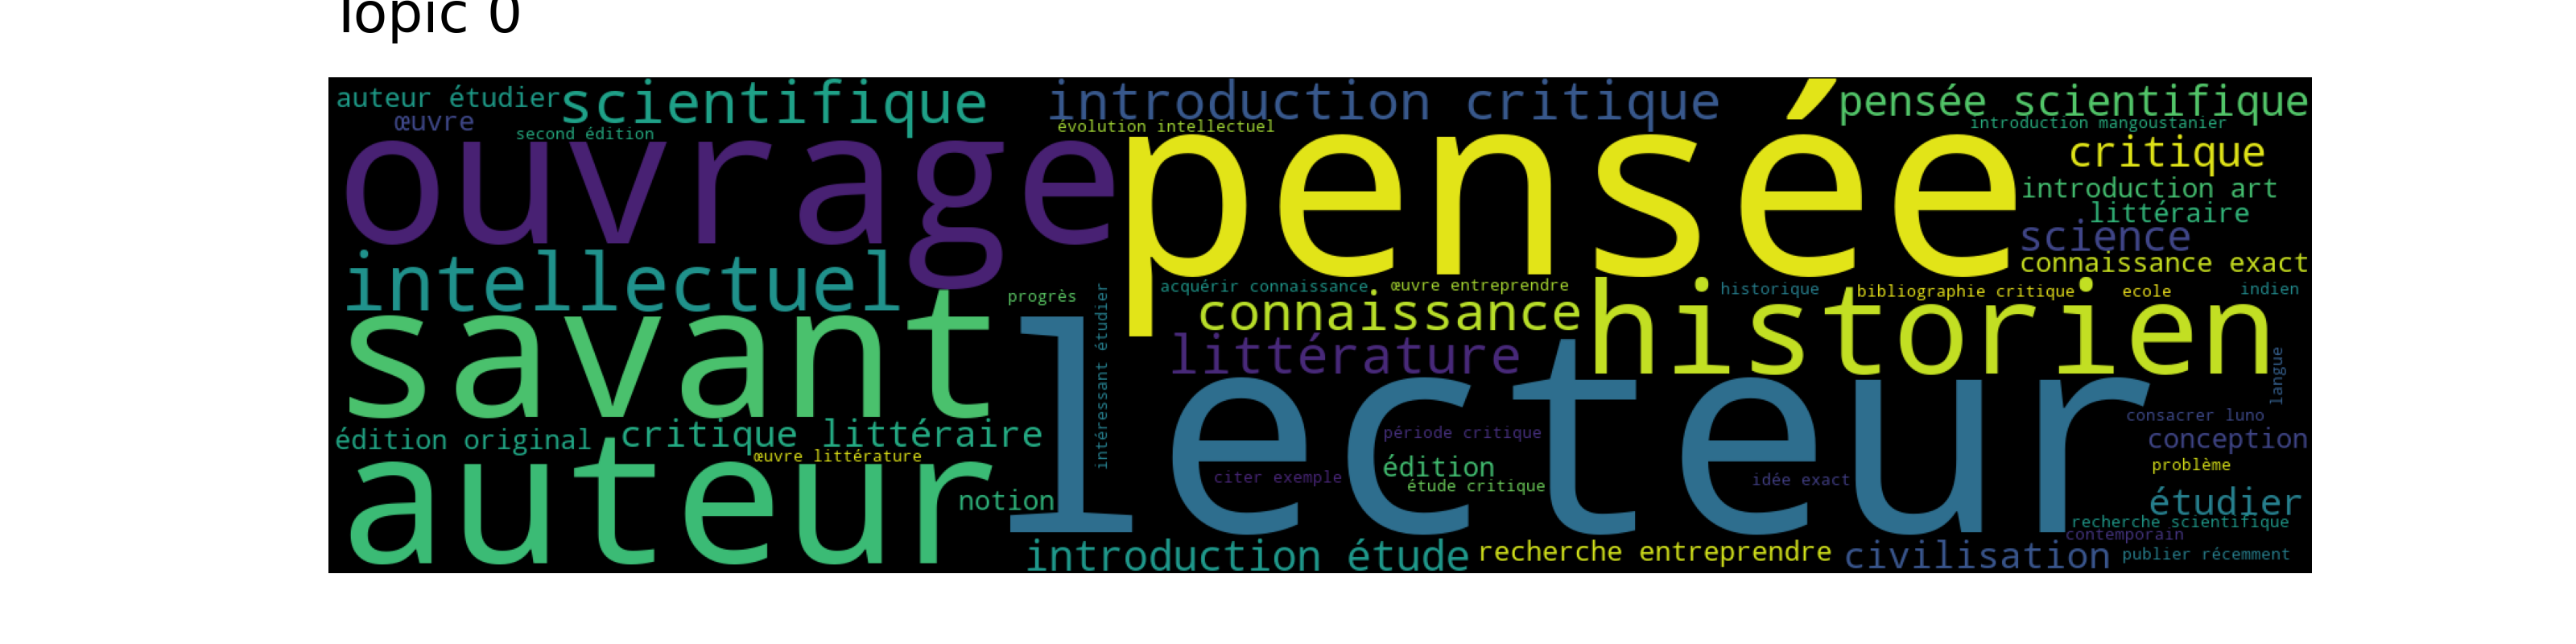
\includegraphics[width=\textwidth]{img/wordcloud model ngram 200 topic 0 .png}
         \caption{Recherche historique et humanité}
         \label{fig:tp12_0}
     \end{subfigure}
     \hfill
     \begin{subfigure}[b]{0.9\textwidth}
         \centering
         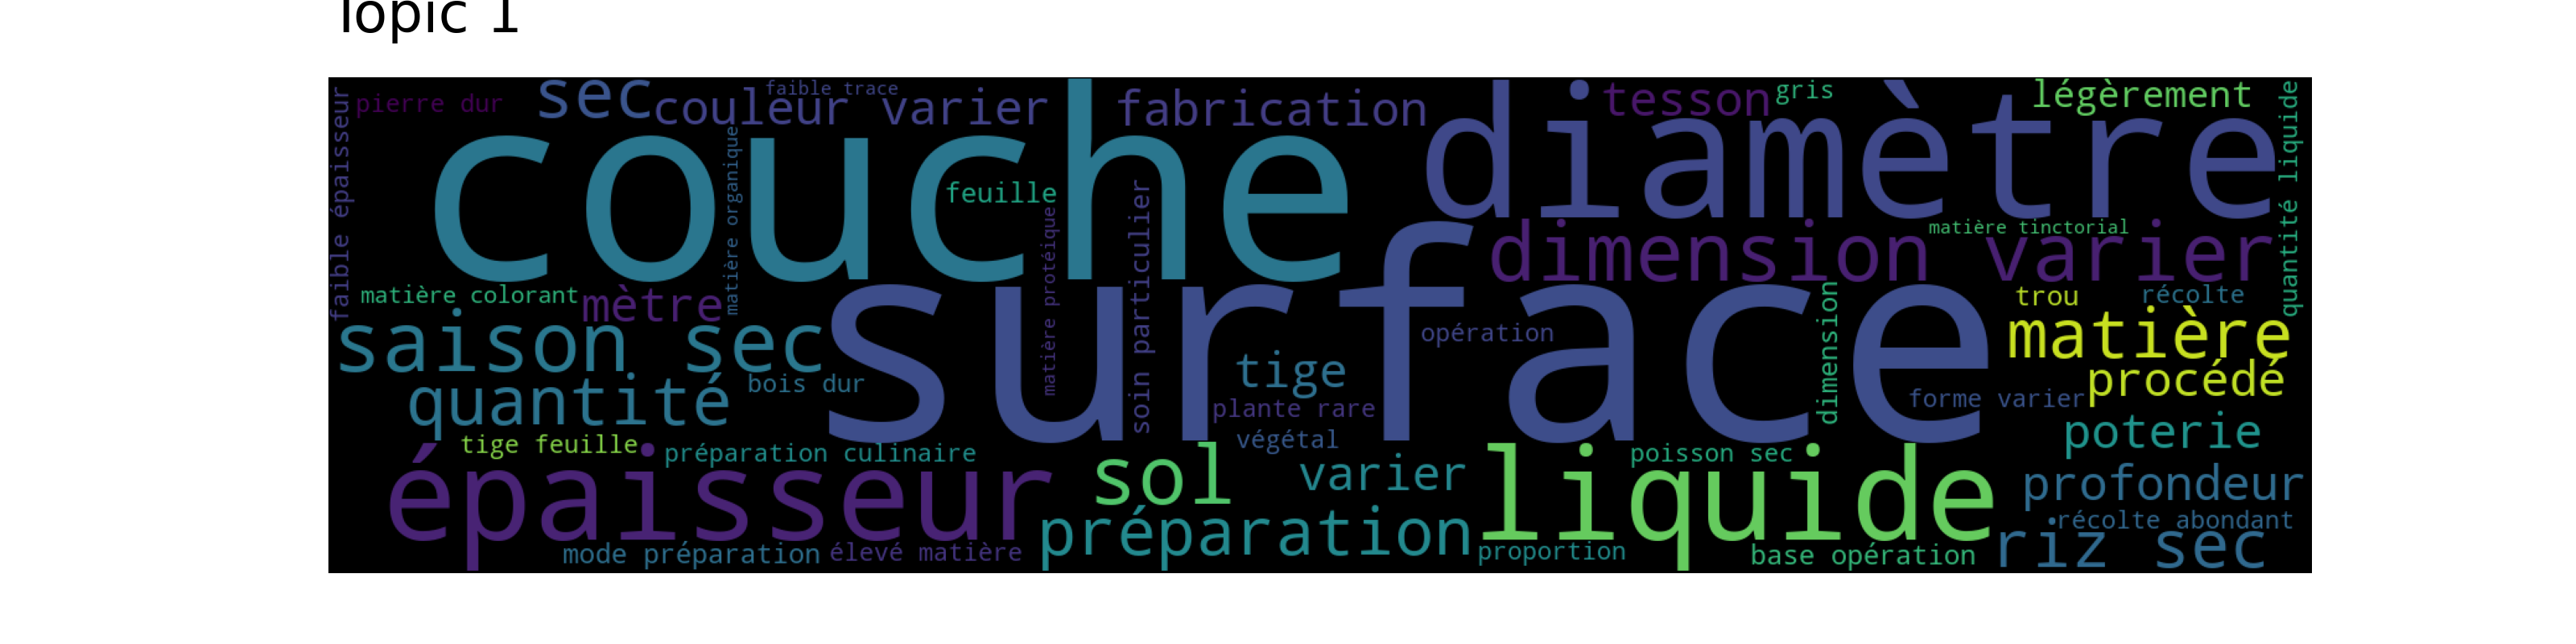
\includegraphics[width=\textwidth]{img/wordcloud model ngram 200 topic 1 .png}
         \caption{Agriculture et Plantation}
         \label{fig:tp12_1}
     \end{subfigure}
     \hfill
        \caption{Les grands sujets du corpus}
    % \label{fig:2_big_topic}
\end{figure}

En outre, certains sujets sont très bien regroupés avec une belle cohérence de contenu dans les documents. La Figure \ref{fig:lao_cam} illustre les nuages de mots pour les sujets "Culture et Architecture Khmer Cambodgien" et "Les ethnies Vietnamiennes/Laotiennes".

\begin{figure}[ht]
     \centering
     \begin{subfigure}[b]{0.9\textwidth}
         \centering
         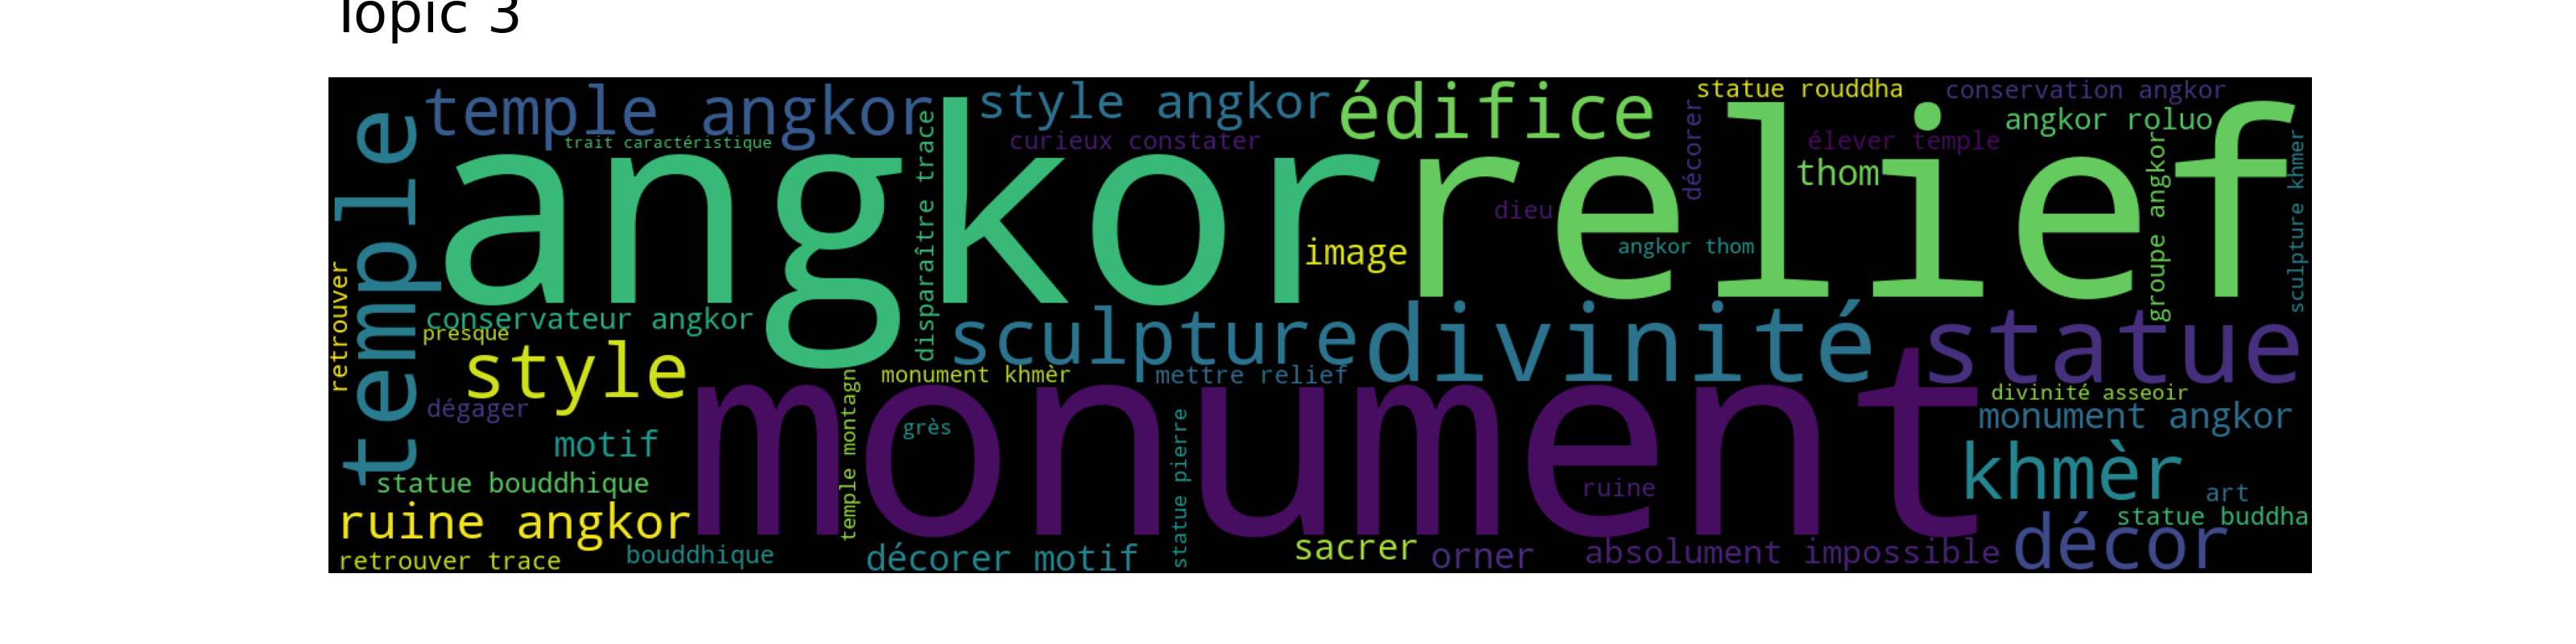
\includegraphics[width=\textwidth]{img/wordcloud model ngram 200 topic 3 .png}
         \caption{Culture et Architecture Khmer Cambodgien}
         \label{fig:tp12_3}
     \end{subfigure}
     \hfill
     \begin{subfigure}[b]{0.9\textwidth}
         \centering
         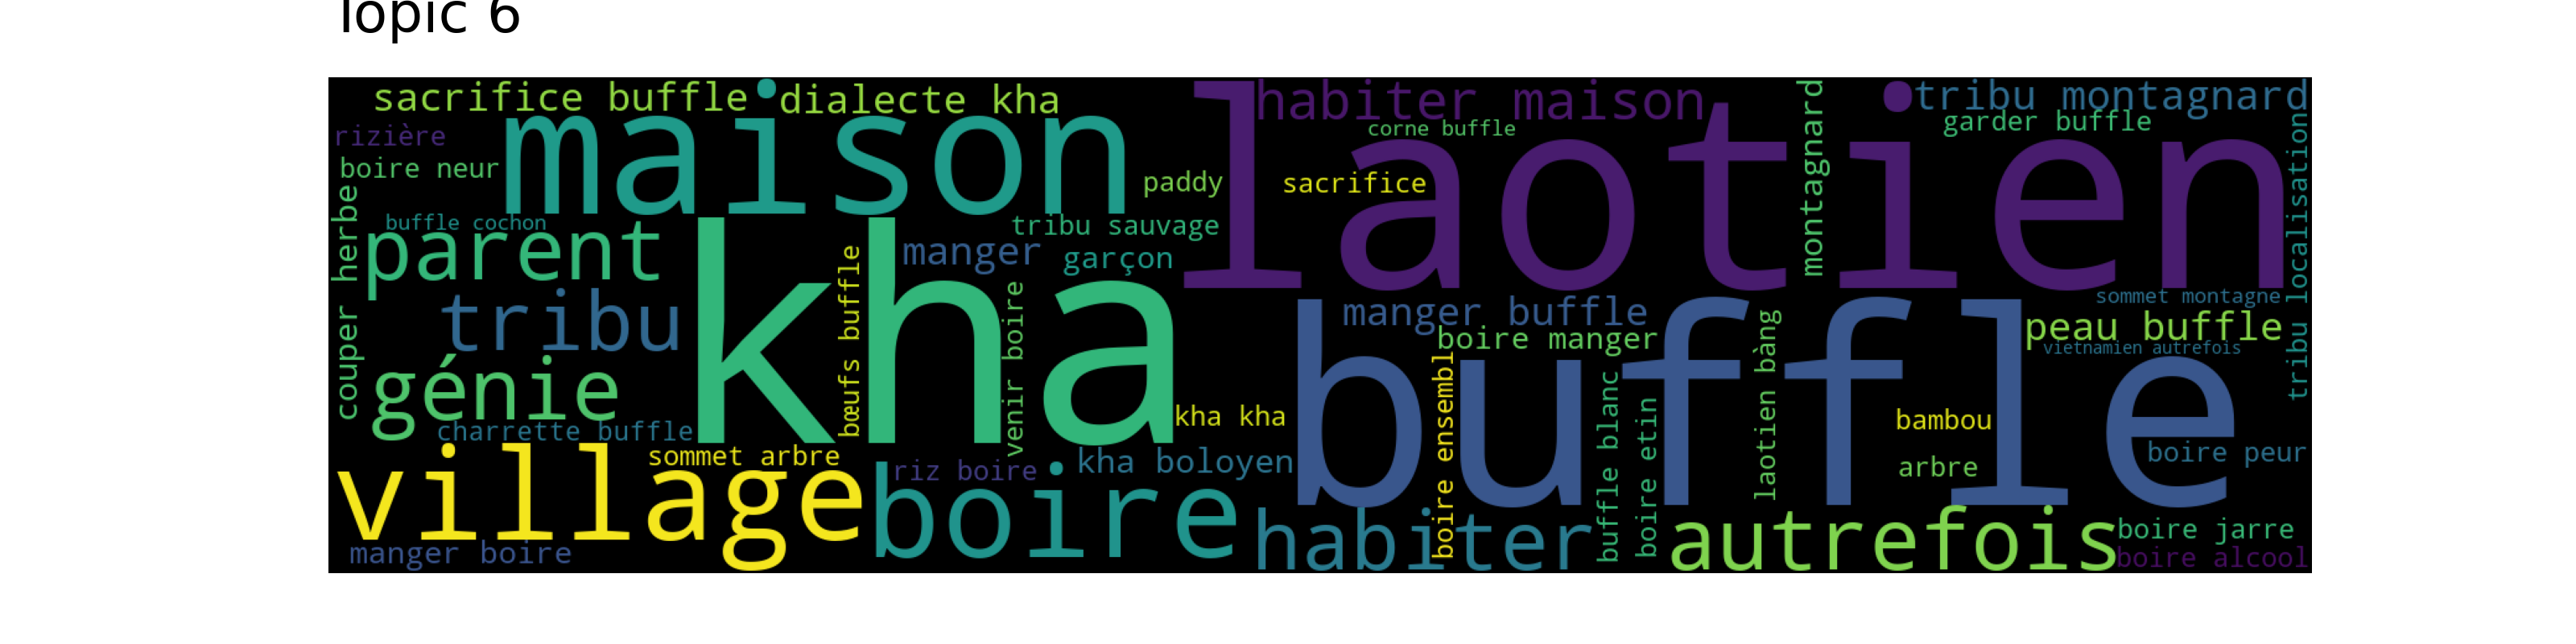
\includegraphics[width=\textwidth]{img/wordcloud model ngram 200 topic 6 .png}
         \caption{Les ethniques Vietnamiens/Laotiens}
         \label{fig:tp12_6}
     \end{subfigure}
     \hfill
        \caption{Les sujets de Laos/ Cambodge}
        \label{fig:lao_cam}
\end{figure}

La Figure \ref{fig:vie_chn} met en évidence deux groupes de documents qui sont regroupés principalement en fonction des langues autres que le français qui coexistent dans les textes. Dans ce cas, le modèle tient compte de la présence de mots étrangers qui apparaissent fréquemment, plutôt que du contenu réel des sujets. Dans le nuage de mots des documents chinois, on trouve de nombreux noms en Pinyin qui n'apportent aucune signification. Cependant, il y a deux mots clés importants, "graver" et "antique", qui proviennent d'un grand article sur la sigillographie chinoise. Malheureusement, il y a également de bons articles sur la médecine traditionnelle et des récits sur les rois vietnamiens qui sont mal classés dans la liste des documents.

\begin{figure}[h]
     \centering
     \begin{subfigure}[b]{.9\textwidth}
         \centering
         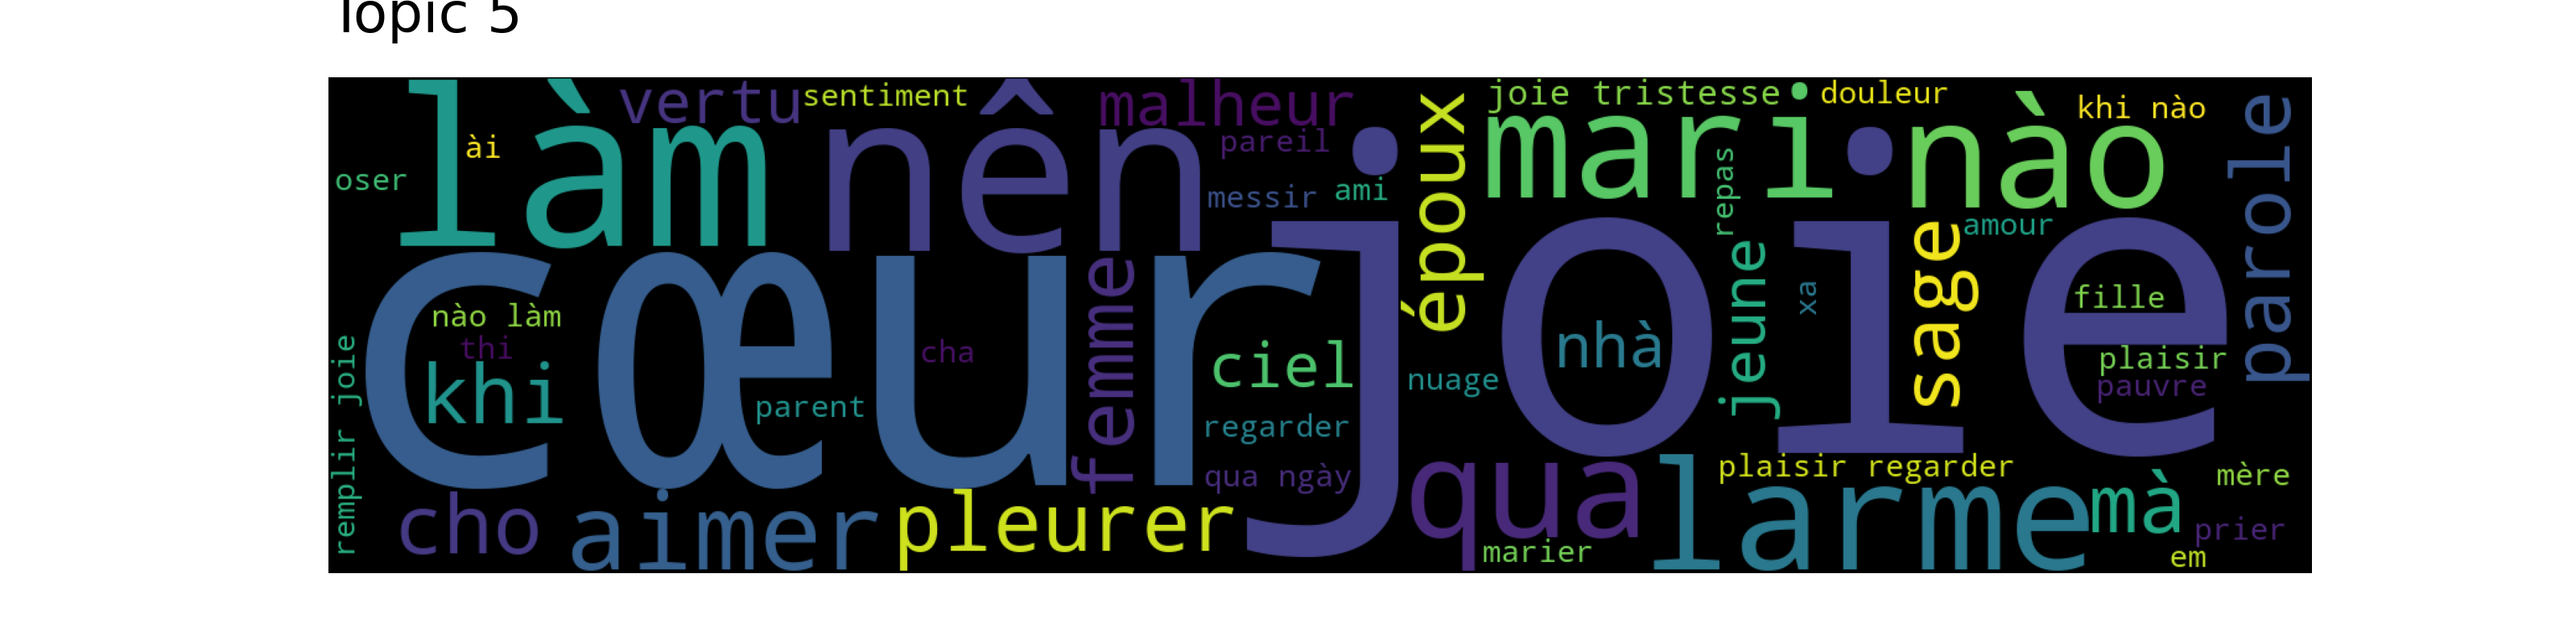
\includegraphics[width=\textwidth]{img/wordcloud model ngram 200 topic 5 .png}
         \caption{Traduction/Bilingue Vietnamien}
         \label{fig:tp12_5}
     \end{subfigure}
     \hfill
     \begin{subfigure}[b]{.9\textwidth}
         \centering
         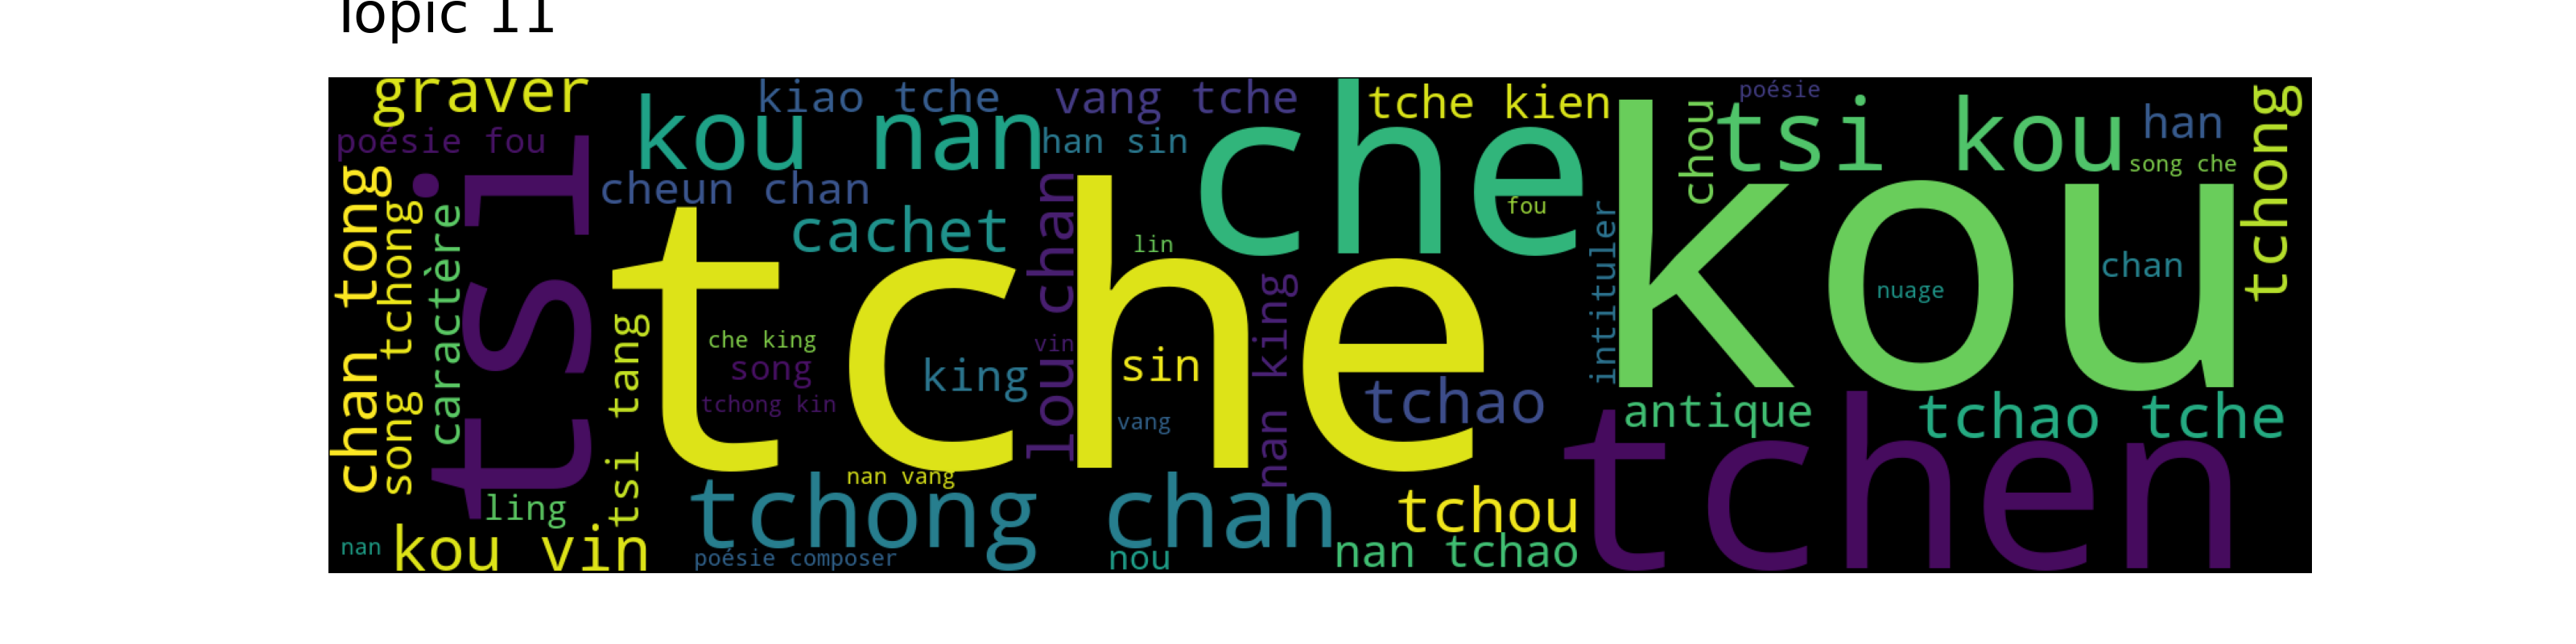
\includegraphics[width=\textwidth]{img/wordcloud model ngram 200 topic 11 .png}
         \caption{Traduction/Bilingue Chinoise}
         \label{fig:tp12_11}
     \end{subfigure}
     \hfill
        \caption{Les documents billingue ou les traductions}
        \label{fig:vie_chn}
\end{figure}

Un autre type de regroupement considéré comme un mauvais regroupement est illustré dans la Figure \ref{fig:noise_topic}, où le modèle a évalué des documents tels que les couvertures, les tables des matières, les avis, les listes de membres, les listes de sociétés correspondantes, ou encore les rapports d'activités trimestriels ou annuels de la société, comme des sujets principaux. Cela souligne également une faiblesse d'un modèle entraîné avec des bigrams, car il met en avant des collocations répétitives dans le texte, telles que "société de géographie", "directeur général", "activité de la société", alors que ces documents sont généralement courts et n'apportent pas suffisamment de contributions sémantiques. Nous considérons ces types de sujets comme du bruit.

\begin{figure}[H]
     \centering
     \begin{subfigure}[b]{0.9\textwidth}
         \centering
         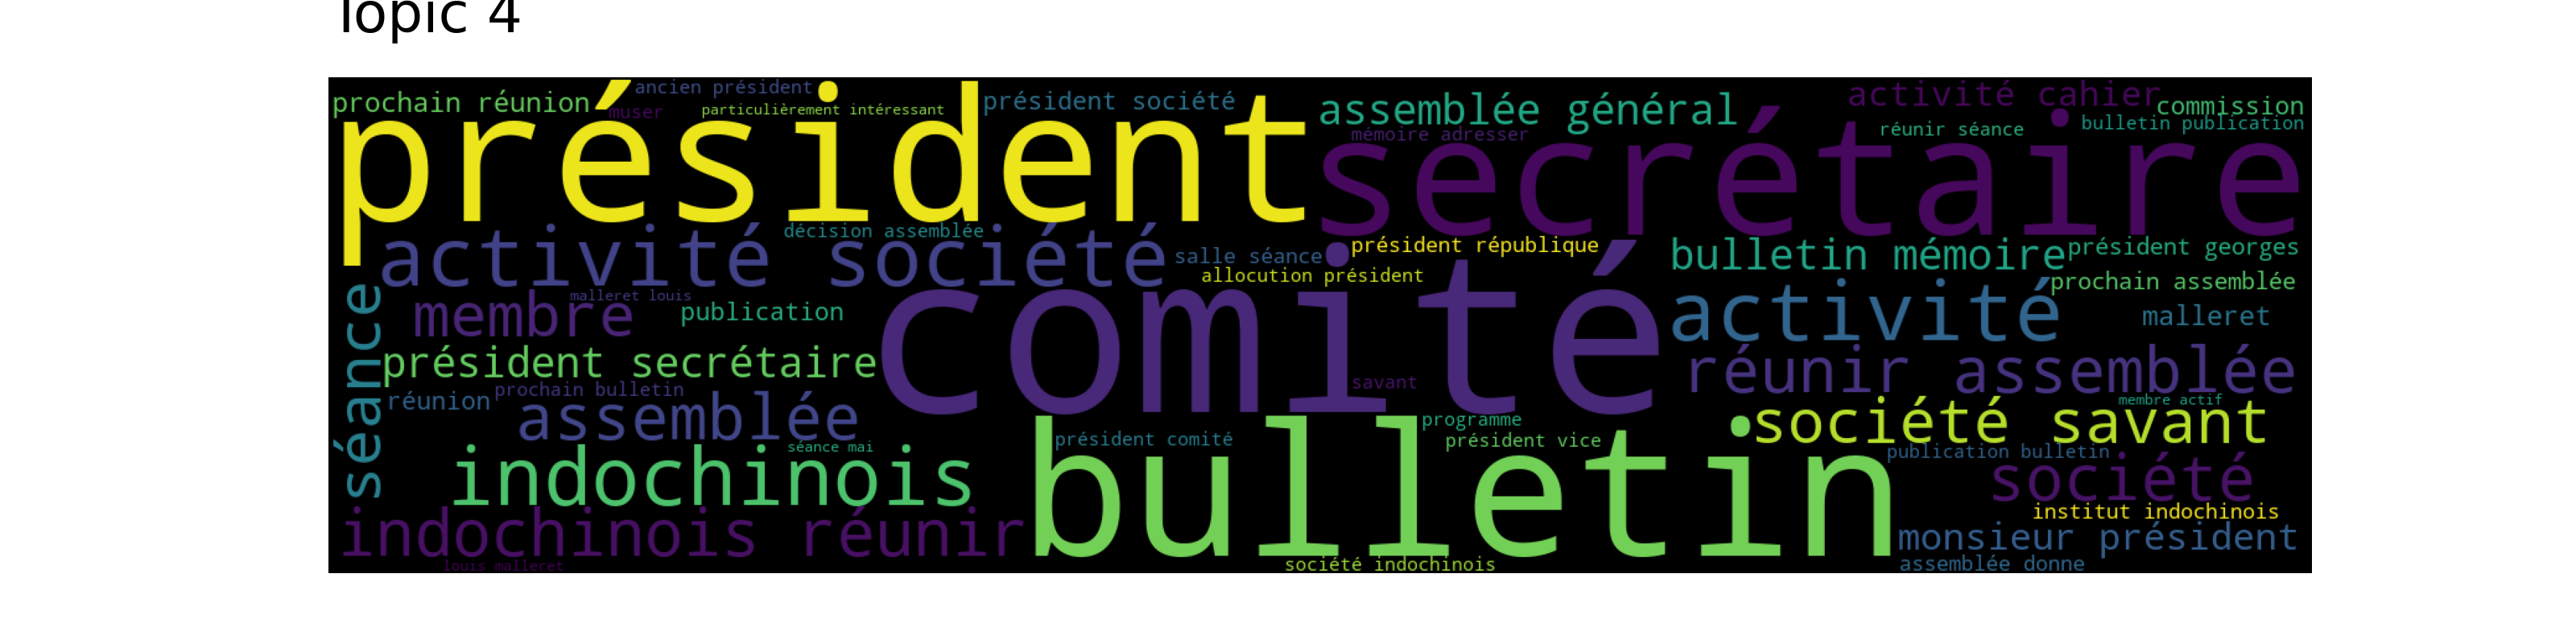
\includegraphics[width=\textwidth]{img/wordcloud model ngram 200 topic 4 .png}
         \caption{Assemblee generale, allocution president}
         \label{fig:tp12_4}
     \end{subfigure}
     \hfill
     \begin{subfigure}[b]{0.9\textwidth}
         \centering
         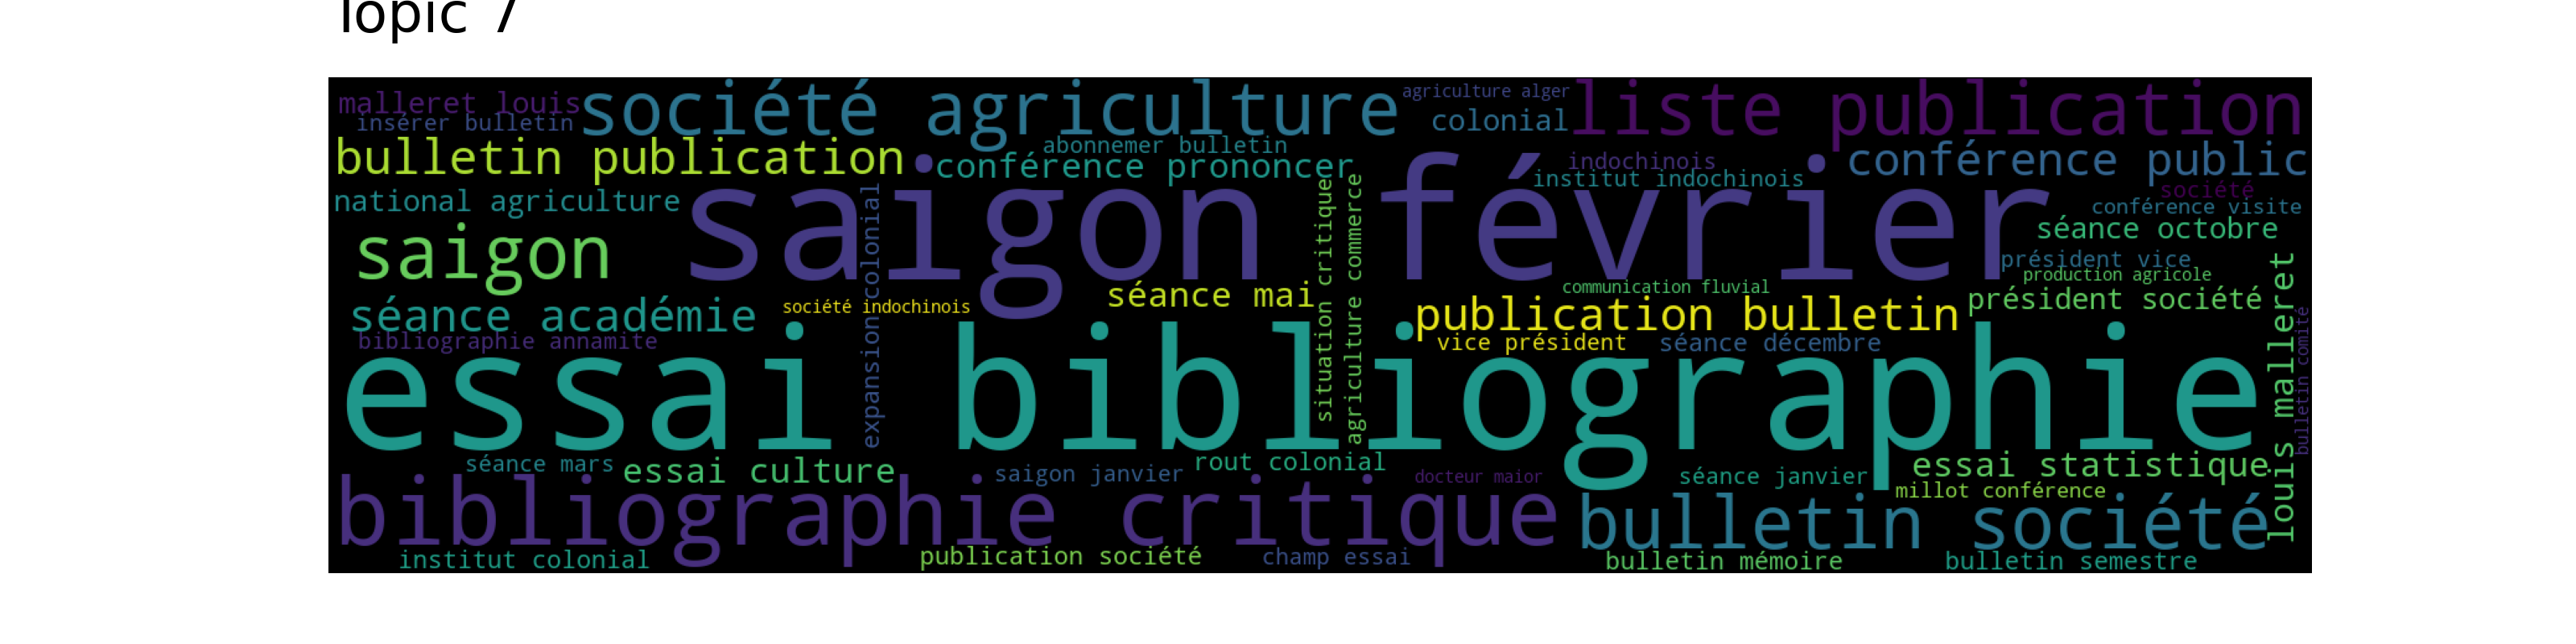
\includegraphics[width=\textwidth]{img/wordcloud model ngram 200 topic 7 .png}
         \caption{Couverture, tables de matiere, avis, liste des membres}
         \label{fig:tp12_7}
     \end{subfigure}
     \hfill
     \begin{subfigure}[b]{0.9\textwidth}
         \centering
         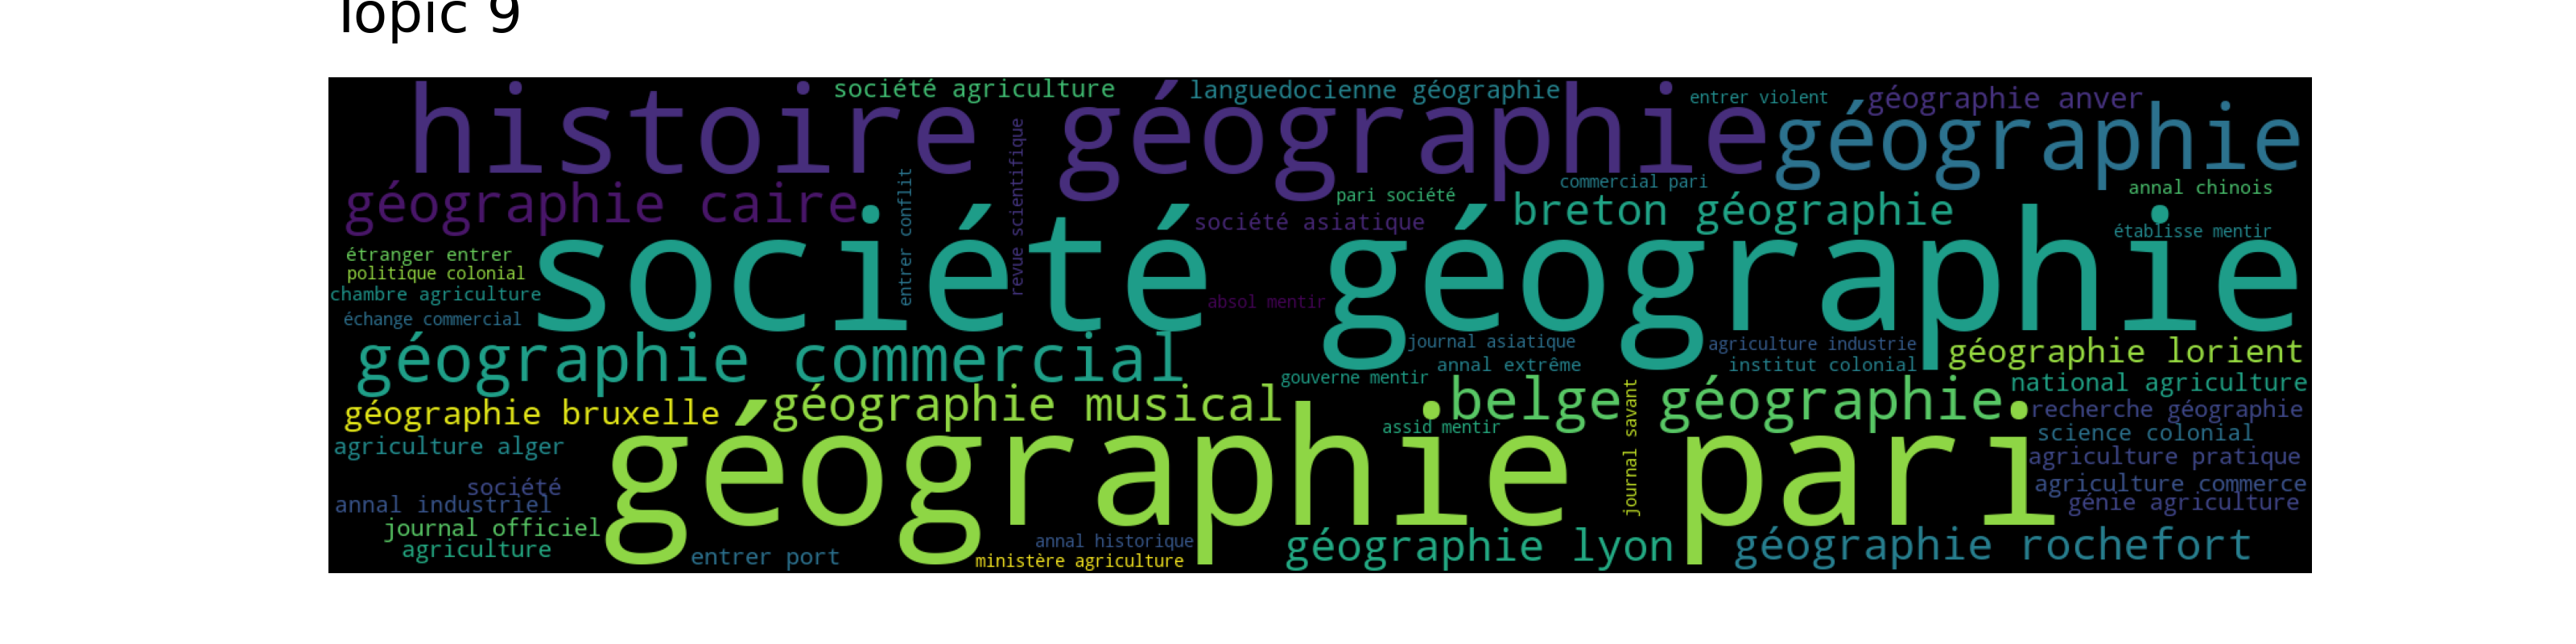
\includegraphics[width=\textwidth]{img/wordcloud model ngram 200 topic 9 .png}
         \caption{Catalogues, listes des correspondantes}
         \label{fig:tp12_9}
     \end{subfigure}
        \caption{Les sujets du bruit}
        \label{fig:noise_topic}
\end{figure}

Les vecteurs associés à chaque document peuvent être représentés visuellement en utilisant une projection UMAP, de manière similaire à ce qui est montré sur la Figure \ref{fig:umap12}. Dans cette représentation, les points symbolisent les segments et sont colorés en fonction de leur sujet principal. Une observation importante est la prédominance de quatre sujets principaux : "recherche générale", "agriculture et plantation", "militaire" et "architecture cambodgienne". Les vecteurs du sujet "recherche générale" se positionnent au centre de l'espace où l'on peut également trouver les vecteurs des autres groupes, un peu comme dans la zone des documents militaires. En revanche, les documents relatifs aux sujets "agriculture" et "architecture cambodgienne" sont assez distinctifs et se trouvent en périphérie de l'espace.

\begin{figure}[t]
    \centering
    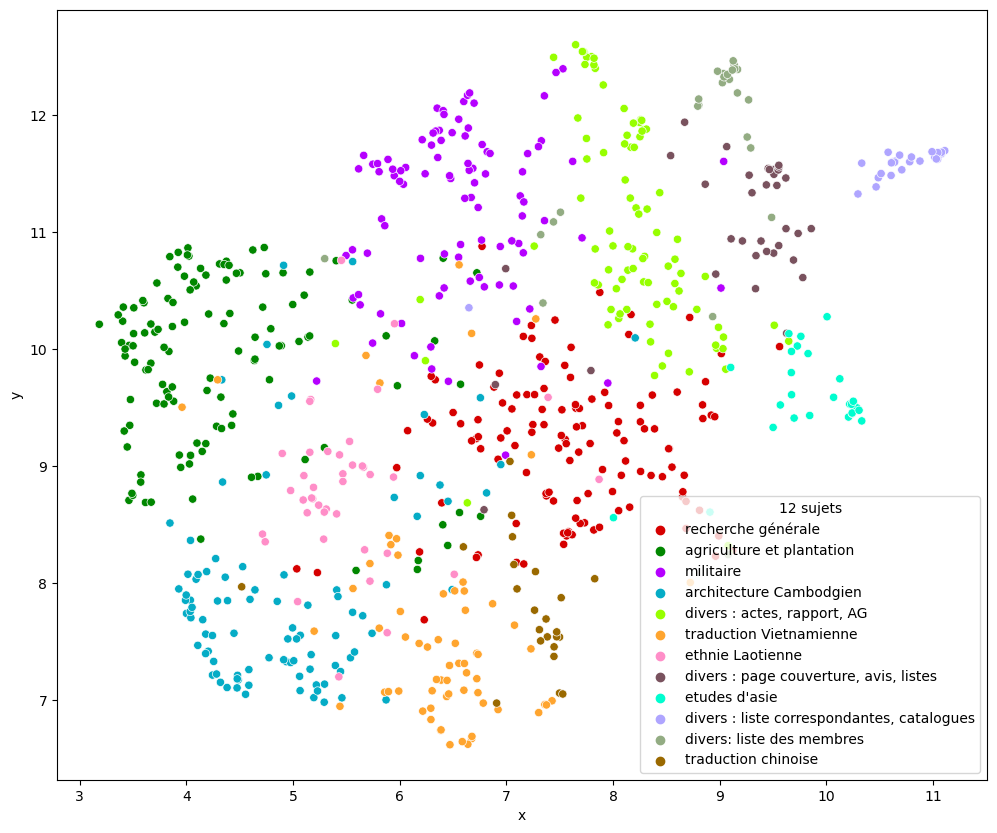
\includegraphics[width=13cm]{img/12umap.png}
    \caption{Distribution spatial des sujets}
    \label{fig:umap12}
\end{figure}

\subsection{Discussion}
Dans cette section, nous présentons deux modèles thématiques qui s'appliquent directement à notre corpus. Contrairement à LDA, une méthode traditionnelle que nous avions initialement envisagée pour la classification de documents, mais qui n'a pas produit de résultats clairs, Top2Vec a rapidement démontré sa supériorité en offrant une compréhension significative de la structure sémantique de ses thèmes. 

En conséquence, nous avons choisi d'exploiter Top2Vec pour approfondir nos recherches dans ce projet. Malgré une analyse approfondie des sujets, certaines limites subsistent. Notre objectif est donc de minimiser autant que possible les thèmes moins pertinents, afin de nous concentrer sur la sélection des textes les plus essentiels qui contribuent à la réputation de ce magazine.

En outre, un autre défi que nous rencontrons avec Top2Vec concerne la tendance des grands sujets à englober un large éventail de petits domaines de recherche, ce qui complique la création de sujets plus précis. Malgré nos nombreux essais avec différents paramètres, nous n'avons pas réussi à obtenir plus que le nombre correct de sujets. 

De plus, en dehors de quelques sujets principaux comme "Agriculture", "Militaire" ou bien "Architecture", chaque exécution de l'apprentissage automatique génère un modèle différent, ce qui pose des problèmes en termes de reproductibilité, similaire à de nombreux modèles d'apprentissage aléatoire. Notre tâche consistera donc à développer une méthodologie de recherche capable de systématiquement identifier les documents liés à chaque sous-thème de manière cohérente.

% Il est également intéressant d'examiner la répartition des sujets au fil du temps à l'époque, la figure \ref{fig:topic_time} présente cet aspect. On peut immédiatement remarquer une distribution inversée dans le temps entre le sujet 6 et le sujet 8. Le sujet 0, composé de sujets liés à l'histoire, à la recherche et à la littérature, est très rare avant 1920, lorsque la colonie indochinoise était encore en cours d'installation. Le sujet 6, qui concerne les traductions et les textes vietnamiens, n'apparaît que après les années 1945, tandis que le sujet 8, qui englobe les documents du gouvernement, se trouve principalement au début du régime colonial de l'époque. On peut également noter que le sujet militaire est plus concentré autour de l'année 1945, une période particulièrement importante de la guerre de libération au Vietnam et en Indochine. Les documents sur l'agriculture (sujet 1) sont moins présents entre 1910 et 1950.

% \begin{figure} %[!ht]
%     \centering
%     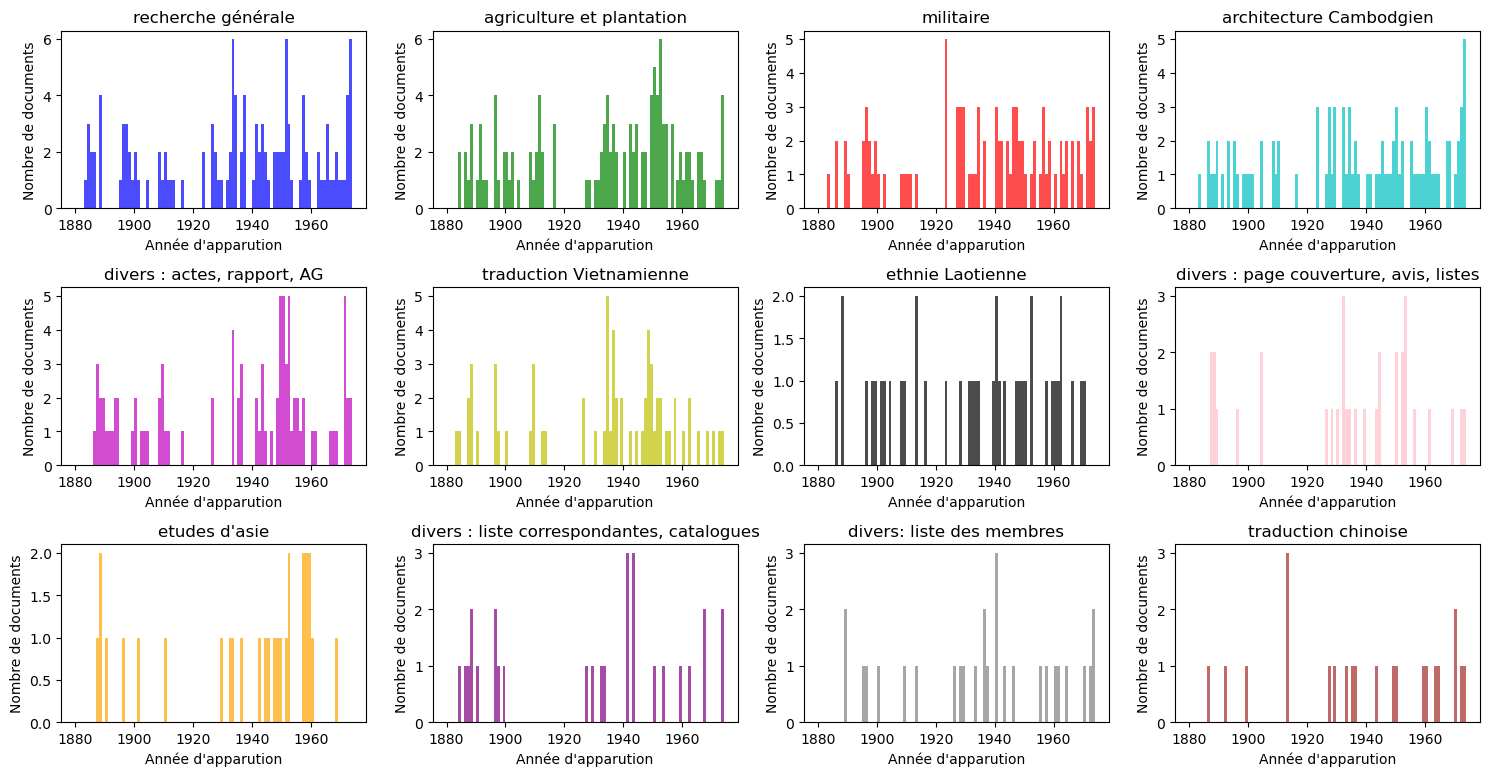
\includegraphics[width=14cm]{img/12temp.png}
%     \caption{Distribution temporelle des sujets}
%     \label{fig:topic_time}
% \end{figure}

\clearpage
\newpage
% \mbox{~}
% \clearpage
% \newpage

\section{Amélioration du modèle de regroupement}
Dans cette section, nous allons proposer deux approches pour améliorer le regroupement des sujets. La première approche est dirigée directement de nos observations quand nous avons constaté qu'une part importante des documents divers sont identifiés comme un sujet en raison de la répétition fréquente de certains vocabulaires ou de la similarité structurelle et de longueur entre ces documents. La présence de ces documents dans le corpus peut influencer le regroupement. Comme ces contenus de documents ne contribuent pas beaucoup de significations, nous avons décidé de les éliminer du corpus en les filtrant par les titres de documents. 

Les résultats de la première approche seront discutés, et il apparaît que le modèle n'arrive toujours pas à distinguer différentes disciplines scientifiques dans le corpus. Un autre problème réside dans les articles qui mélangent le français et une autre langue, souvent le vietnamien ou le chinois, et qui peuvent parfois inclure de véritables articles sur d'autres sujets.
C'est pourquoi nous proposons la deuxième approche, qui consiste à utiliser Word2Vec. Ce modèle est capable de rechercher une liste de mots-clés, et un modèle Top2Vec qui s'entraîne  sur un espace de mots plus large pourrait alors extraire les documents pertinents pour chaque mot-clé. 
Une analyse de cette méthode de recherche sera apportée en fin de la section.

\subsection{Avec un corpus pré-filtré}
\subsubsection{Suppression des documents moins pertinents}
Pour réduire l'impact des documents divers liés à l'administration ou à l'organisation de la société B.S.E.I, nous allons les filtrer avant de procéder à l'entraînement du corpus. Le tableau \ref{tab:acte_societe} présente une statistique sur la quantité de documents et de mots de ce type de documents. Cette partie représente 10,35 \% de l'ensemble du nombre de documents et 4,24 \% en termes de quantité de mots.
\begin{center}
\begin{tabular}{ |c|c|c| } %{|p{5cm}|p{5cm}|p{4cm}|}
\hline
Titre & Nombre de documents & pourcentage de mots\\
\hline
actes société & 45 & 1.34\%  \\ 
liste membres & 22 &  2.22\%  \\
liste générale membres & 15 & 0.37\%  \\
procès verbaux/verbal & 57 & 0.29\% \\ 
bureau-de-la-société & 15 & 0.37\%  \\
\hline
Total & 139 & 4.24\%  \\
\hline
\end{tabular}
\label{tab:acte_societe}
\end{center}

\subsubsection{Analyse des résultats}

Le modèle a ensuite été ré-entraîné, ce qui a abouti à une nouvelle modélisation réduite à 6 sujets, avec les mots-clés qui sont répertoriés dans le tableau \ref{tab:6topic}.

\begin{center}
\begin{tabular}{|p{15cm}|}
\hline
Regroupement des sujets et les mot-cles\\
\hline
 Sujet 0 : centimètre, sécher, sec, couche, acide, sol, liquide, graine, rendement, quantité, humidité, température, mètre, surface, tige \\ \hline
 Sujet 1 : joie, larme, prosterner, malheur, cœur, ciel, écria, parole, pleurer, époux, mari, messir, hsiuan, bouddha, bonheur \\ \hline
 Sujet 2 : chercheur, pensée, civilisation, savant, synthèse, intellectuel, science, conception, spécialiste, ouvrage, documentation, morale, scientifique, lecteur, connaissance \\ \hline
 Sujet 3 : amiral, frégate, expédition, capitaine, canonnière, navire, marine, commandant, prise, débarquer, artillerie, expéditionnaire, colonie, occupation, conquête \\ \hline
 Sujet 4 : conférence, culturel, indochinois, président, activité, société, étude, comité, membre, programme, savant, ecole, congrès, secrétaire, bibliothèque \\ \hline
 Sujet 5 : monument, sculpture, statue, relief, sanctuaire, angkor, khmèr, décoratif, édifice, linteau, architecture, art, temple, buddha, prei \\ \hline
 Sujet 6 : géographie, société, agriculture, journal, revue, rulletin, society, indo, annal, colonial, bulletin, savant, colonie, commercial, courrier \\ \hline
\end{tabular}
\label{tab:6topic}
\end{center}
% \vspace{1cm}

Le modèle a réussi à former une structure de sujets avec une répartition de documents plus équilibrée, comme le montre la Figure \ref{fig:repartition_7topics}. En observant la répartition en nombre de mots, on constate que les deux sujets "Vie et Religieux" et "Militaire" contiennent beaucoup plus de texte que les autres sujets. En effet, parmi les documents du sujet "Militaire", on a trouvé que deux sur trois étaient de grandes traductions du roman historique "Les Trois Royaumes", qui relate une longue période de guerre en Chine et qui est classé parmi les romans les plus longs et les plus anciens de l'histoire chinoise.

\begin{figure*}[]
    \centering
    \begin{subfigure}[t]{0.45\textwidth}
        \centering
        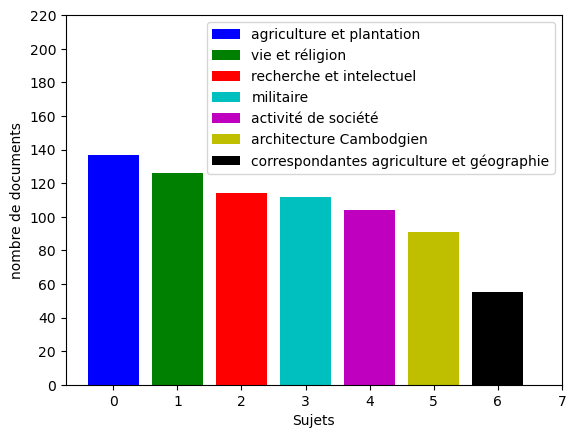
\includegraphics[height=1.9in]{img/6topic_size_docs.png}
        \caption{Répartition de documents}
    \end{subfigure}%
    ~ 
    \begin{subfigure}[t]{0.45\textwidth}
        \centering
        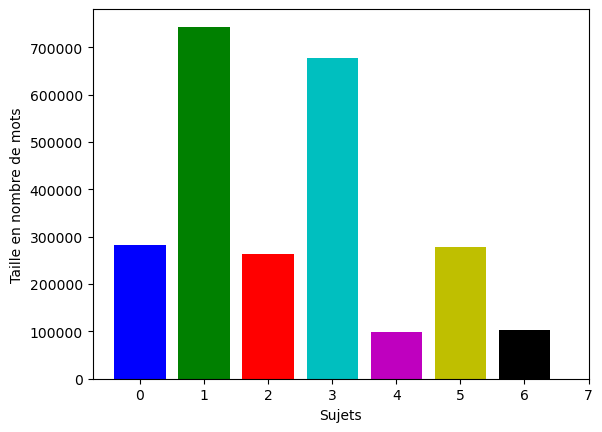
\includegraphics[height=1.9in]{img/6topic_size_words_true.png}
        \caption{Répartition de mots}
    \end{subfigure}
    \caption{Répartition entre les sujets}
    \label{fig:repartition_7topics}
\end{figure*}

En revanche, les documents liés aux activités et aux sociétés correspondantes contiennent très peu de texte dans leurs documents mais malgré tout ils sont bien regroupés par la similarité de leur nature et aussi de leur vocabulaire.

% \begin{figure}[H] %[!ht]
%     \centering
%     \includegraphics[width=14cm]{img/wordcloud filter 2 model ngram 200 topic 0 .png}
%     \caption{WordCloud du sujet }
%     \label{tp0}
% \end{figure}

\begin{figure}[H] %[!ht]
    \centering
    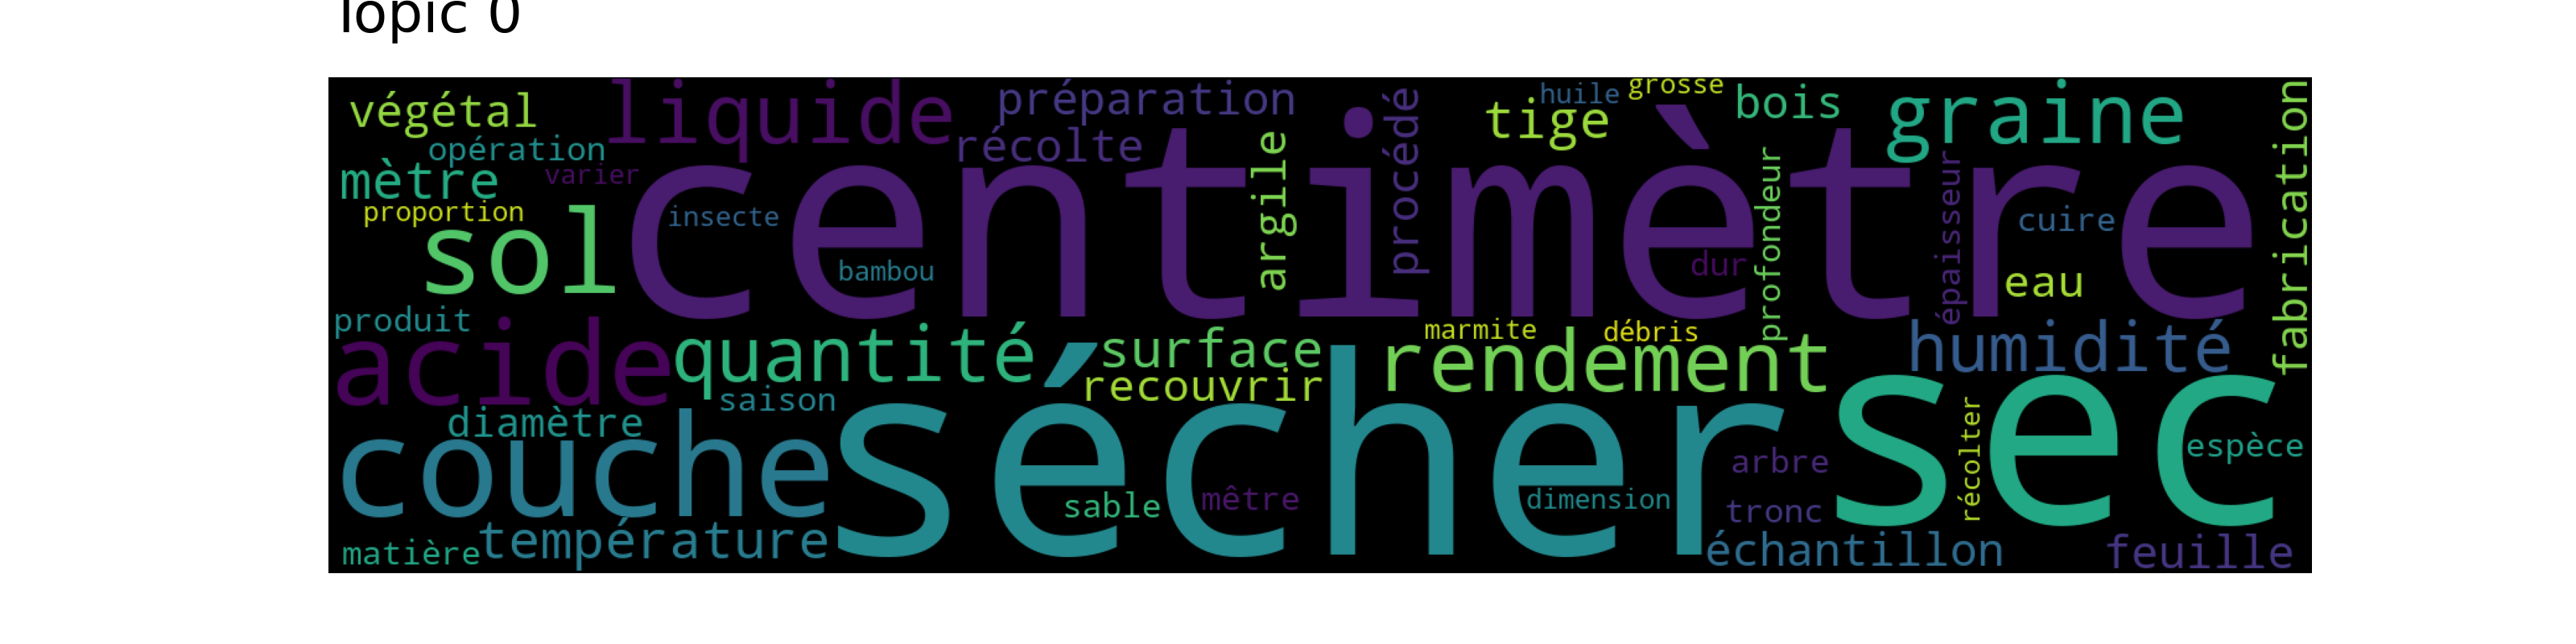
\includegraphics[width=14cm]{img/final_6_topic 0 .png}
    \caption{Agriculture, plantation, alimentation }
    \label{tp0}
\end{figure}
\textbf{Topic 0}: Agriculture, plantation, alimentation\newline
Quelques documents de référence  : 
\begin{itemize}
    \item 
Etudes des minéraux lourds de quelques sables littoraux par Hoang Ngoc Can 1964
    \item 
Résultats des mesures de la température des eaux marines par Hoang Ngoc Can 1964

    \item 
Au sujet des tectes de Dalat par Mailles 1934
    \item 
Compte rendu analytique sur les courants terrestres par Lourme 1883

    \item 
Rapport sur la fabrication de l'acool de riz en Cochinchine par Lévie 1883

    \item 
L'industrie du décortiage du riz en Basse-Cochinchine par Passerat de la Chapelle 1901

    \item 
La poterie dans le Sud-Cambodge par A. Souyris Rolland 1950
\end{itemize}

Les nuages de mots associés à chaque sujet reflètent de manière cohérente l'identité de chaque sujet. En effet, le Bulletin du Comité agricole et industriel de la Cochinchine, en tant que prédécesseur, avait une orientation centrée sur l'agriculture et la culture, et ces thèmes continuent de prédominer dans l'ensemble du corpus. Le premier thème, en particulier, est composé d'articles scientifiques axés sur la recherche en agriculture en Indochine. Les mots-clés révèlent une diversité de cultures tropicales, ainsi que des éléments naturels fondamentaux tels que le sol, l'eau, le sable, la saison, l'argile, la température de surface et leurs caractéristiques telles que "sec", "humidité", "acide", "profondeur", "sécheresse", etc. De plus, on trouve des termes liés au processus de production agricole, tels que "préparation", "fabrication", "récolte", "récolter", qui renforcent la cohérence thématique de ce sujet.

% Effectivement, le thème général de l'agriculture couvre une grande variété de nuances et de domaines d'études plus spécifiques qui ne sont pas facilement discernables à partir d'un simple nuage de mots. Les termes techniques tels que "centimètre", "quantité", "diamètres", "dimension", "échantillon" suggèrent une dimension de précision et de mesure au sein de ce domaine.

Il est important de noter que derrière ce sujet général de l'agriculture, il existe des sujets plus spécialisés et des sous-domaines qui nécessitent une recherche plus approfondie pour être pleinement compris. Par exemple, au sein de cette thématique, il est possible de trouver des recherches portant sur les matériaux, l'industrie, voire des aspects tels que l'artisanat, comme la fabrication de céramique. Ces sujets plus spécifiques et ces nuances offrent d'excellents points de référence dans le corpus. Cependant, une analyse plus détaillée et approfondie est nécessaire pour explorer les thèmes sous-jacents et comprendre pleinement la portée de la recherche dans le domaine de l'agriculture en Indochine.

\begin{figure}[H] %[!ht]
    \centering
    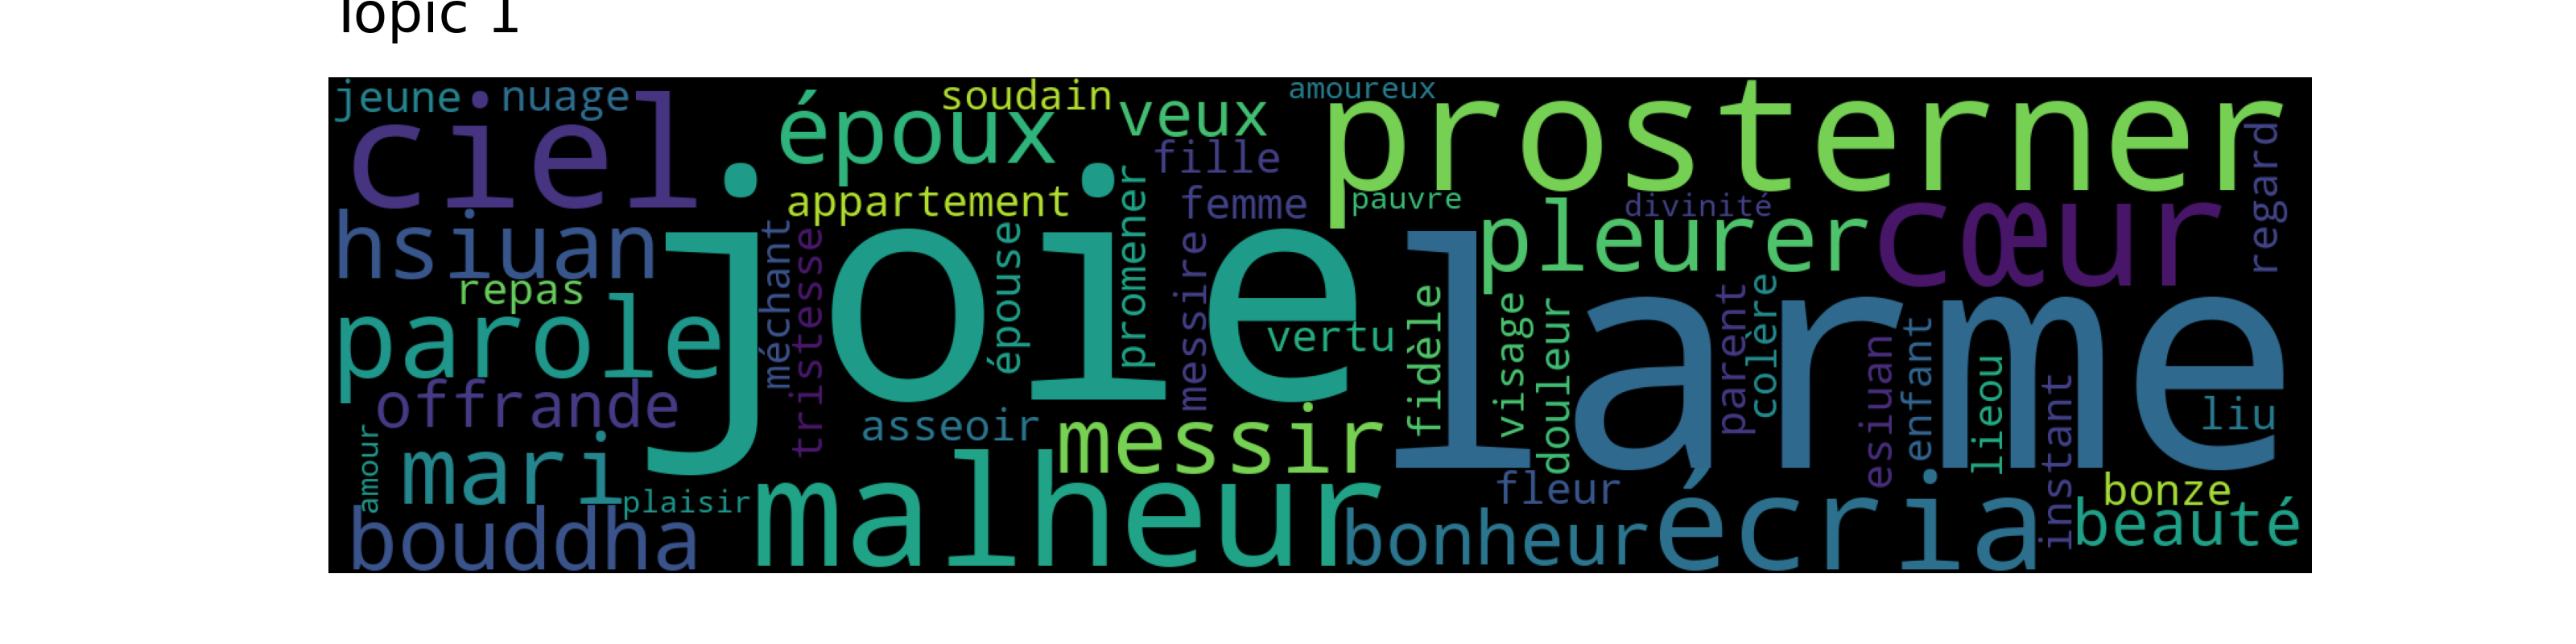
\includegraphics[width=14cm]{img/final_6_topic 1 .png}
    \caption{La vie de famille et religion }
    \label{tp1}
\end{figure}

Topic 1 : La vie de famille et religion

Le bouddhisme et le culte des ancêtres représentent deux des croyances fondamentales du peuple vietnamien, et ils sont intrinsèquement liés à la structure familiale vietnamienne. Les récits et les enseignements religieux sont fréquemment ancrés dans la vie familiale et les émotions humaines. Bien que l'analyse des mots puisse suggérer une prédominance de termes liés aux émotions et à la famille, en réalité, la plupart des articles sur ce sujet sont associés à la dimension religieuse.

"L’Islam est professé par 2\% de la population, 6\% confessent le chris-tianisme et 92\% le bouddhisme. Cette dernière religion est surtout répandue au Camboge et au Laos ; au Viet-Nam, elle est imprégnée de confucianisme"\footcites{truong}


- Topic 2: Intellectuel
\begin{figure}[H] %[!ht]
    \centering
    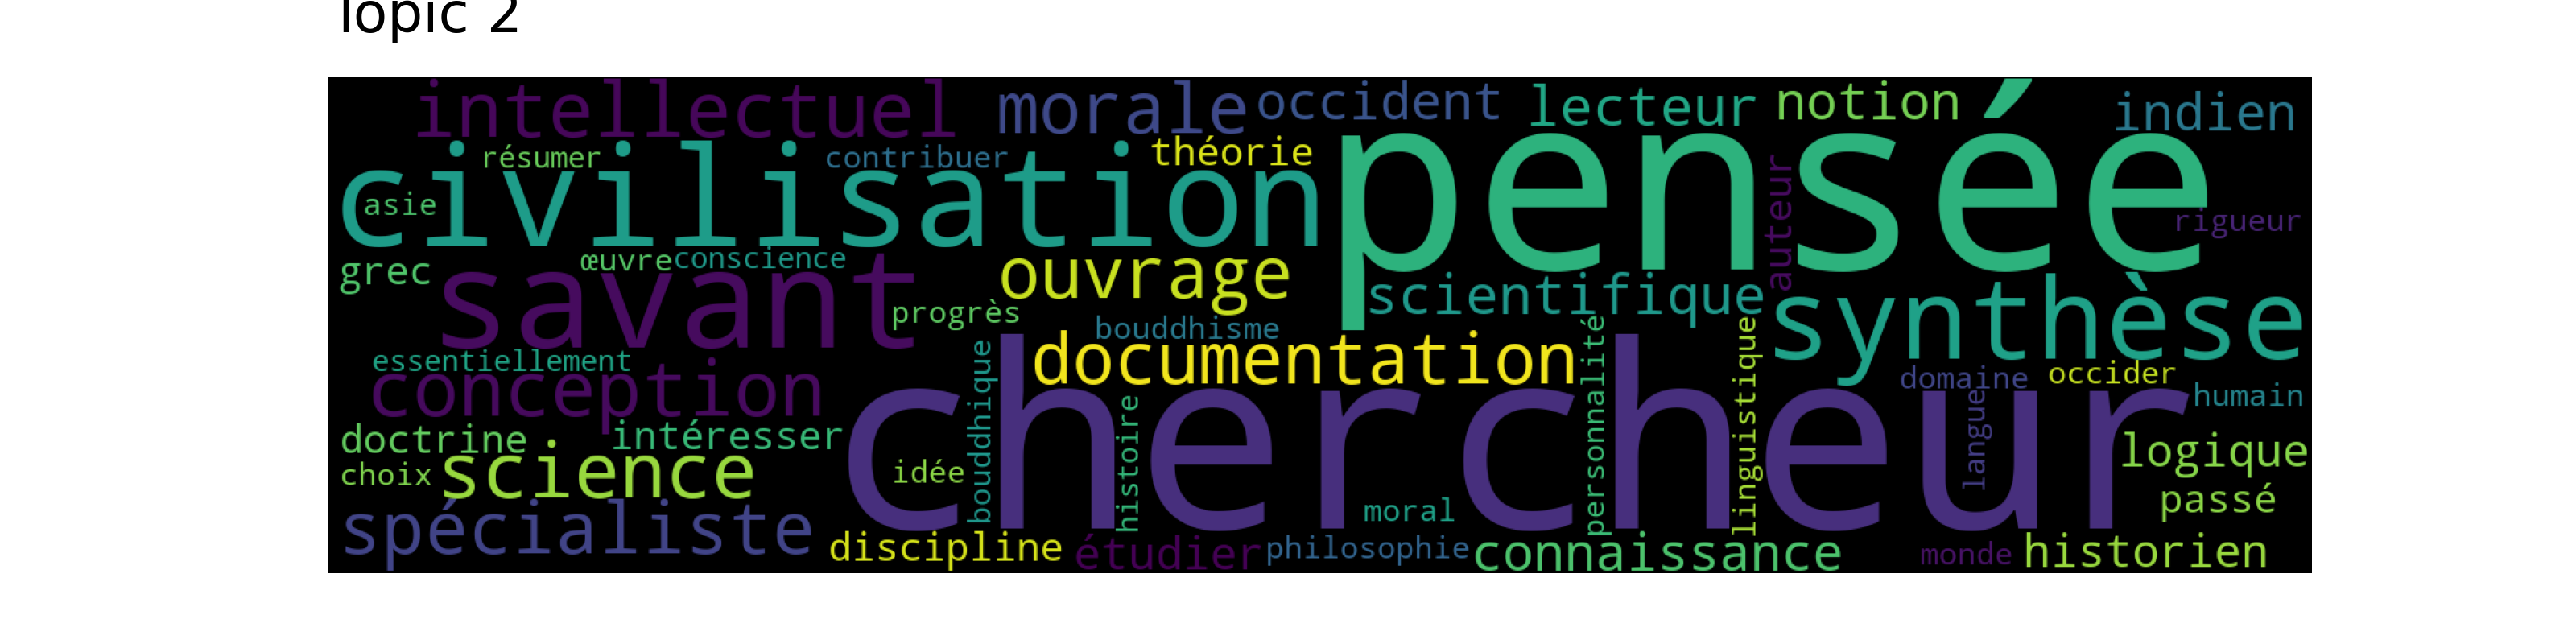
\includegraphics[width=14cm]{img/final_6_topic 2 .png}
    \caption{Intellectuel }
    \label{tp2}
\end{figure}

B.S.E.I reste est une société "savante", car cette expression occupe une place importante dans le deuxième thème du corpus. Ce sujet comprend des sujets intellectuels et scientifiques, des recherches, des essais et des critiques sur l'Indochine. Les discussions tournent autour de sujets autres que l’agriculture
"ouvrage", "documentation", "savant", "intellectuel",  "chercheur", "science", "pensée", "connaissance", "scientifique", "science", synthèse"

Effectivement, il est clair que le B.S.E.I avait un objectif scientifique bien défini et qu'il ne se limitait pas seulement aux articles de recherche scientifique. Il englobait également d'autres types de documents tels que les bibliographies, les catalogues, les publications de l'association et d'autres sociétés savantes. Cette approche montre que le journal avait une vision holistique de la recherche dans l'environnement scientifique et intellectuel de son époque.

En maintenant un réseau complet de documents intellectuels et en répertoriant de manière détaillée les travaux d'autres sociétés savantes, le B.S.E.I a contribué à enrichir les connaissances de ses membres et à promouvoir de nouvelles recherches dans le domaine de l'Indochine. Il a ainsi joué un rôle important dans la diffusion des connaissances et dans la création d'une communauté scientifique dynamique et productive.

Cela montre également que la revue ne se limitait pas à un seul domaine de recherche, mais embrassait une variété de sujets liés à l'Indochine, ce qui contribuait à sa richesse et à sa diversité scientifiques.
Il est important de noter que le magazine restait constamment au courant des développements scientifiques extérieurs et s'efforçait de maintenir son niveau. Cette approche témoigne de l'engagement de la société savante S.E.I. envers la recherche scientifique de haute qualité et son désir de rester à la pointe des avancées dans divers domaines liés à l'Indochine.

En restant à jour avec les développements scientifiques extérieurs, le magazine pouvait non seulement informer ses membres des dernières découvertes et avancées, mais aussi contribuer à la diffusion de ces connaissances au sein de la communauté scientifique indochinoise. Cela renforçait sa réputation en tant qu'organe de diffusion de la connaissance de premier plan dans la région.

En fin de compte, cette approche de maintien du niveau et d'ouverture aux développements extérieurs a contribué à faire du B.S.E.I une revue scientifique de grande qualité et à renforcer son rôle dans la promotion de la recherche en Indochine.

- Topic 3: Militaire
\begin{figure}[H] %[!ht]
    \centering
    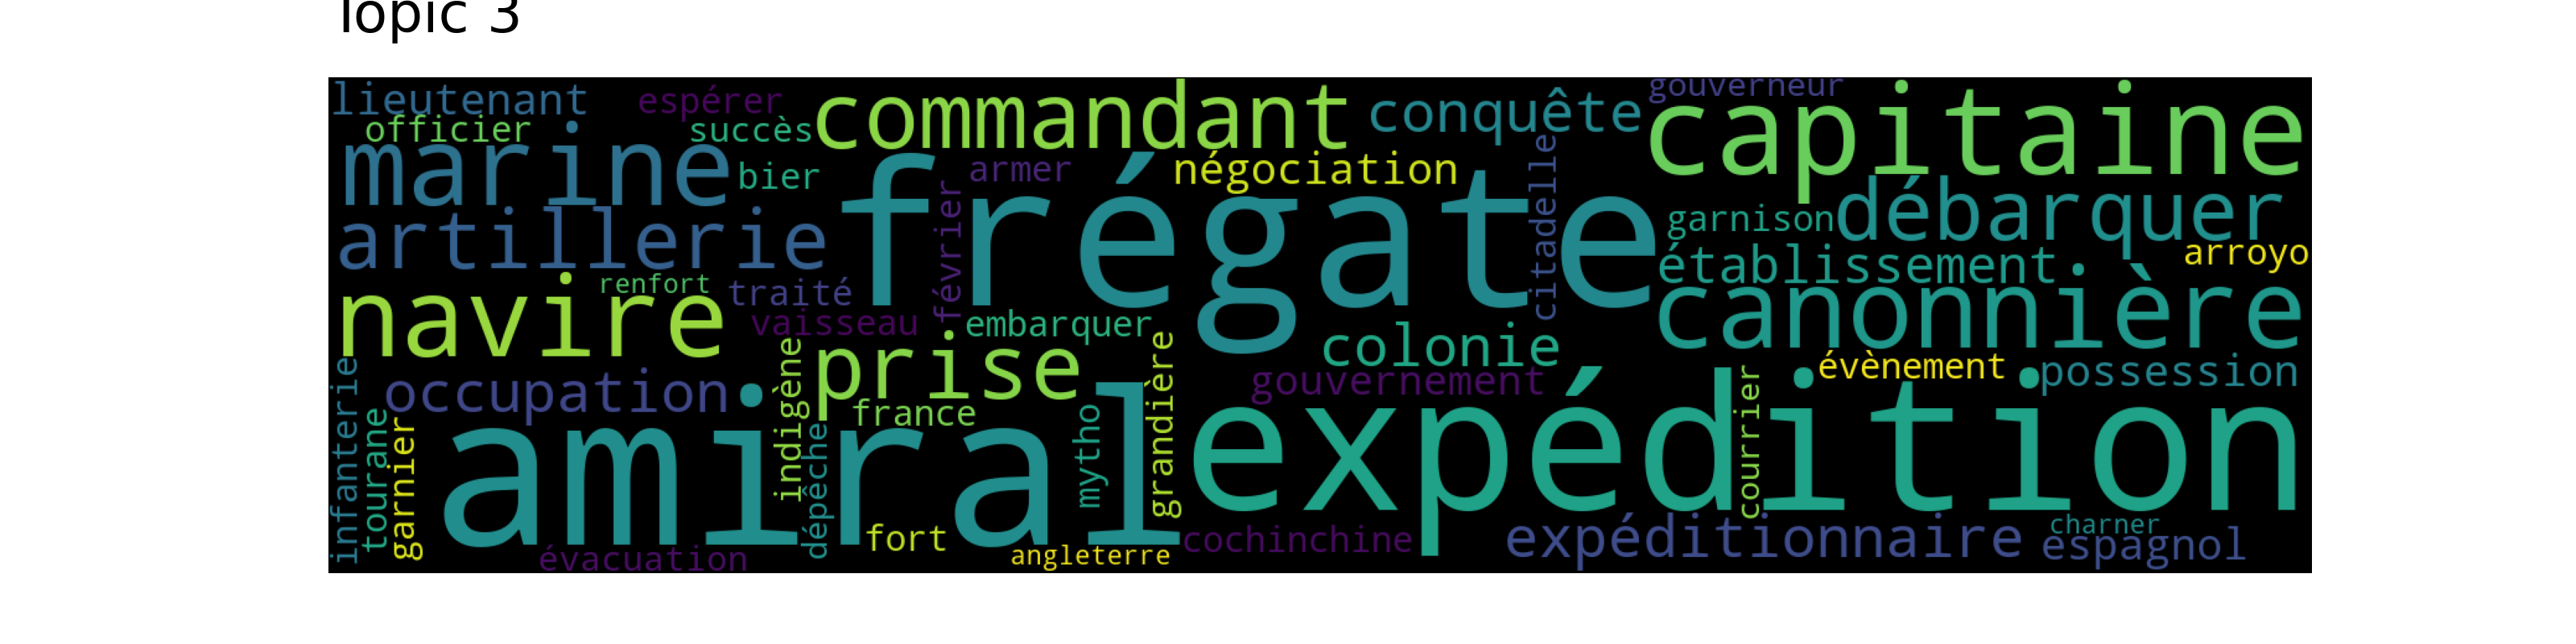
\includegraphics[width=14cm]{img/final_6_topic 3 .png}
    \caption{Document militaire et de la guerre}
    \label{tp3}
\end{figure}

Il est en effet intéressant de noter que, malgré le contexte colonial et les conflits qui ont marqué l'histoire de l'Indochine, la revue B.S.E.I a maintenu une politique de ne pas discuter de politique et de religion. Cela témoigne de sa volonté de se concentrer sur des sujets scientifiques et de recherche, plutôt que de s'engager dans des débats politiques ou religieux.

Le fait que les thèmes liés au militaire dans le nuage de mots comprennent principalement des études sur l'histoire de l'Indochine, les relations passées et les guerres avec les pays voisins est également intéressant. Cela montre que le journal a abordé ces sujets d'un point de vue historique et académique, plutôt que de prendre position sur des questions politiques contemporaines.

Il est également notable que des séries telles que Les trois royaumes ont été abordées dans le journal, ce qui démontre la diversité des sujets traités dans B.S.E.I et son engagement envers la recherche et la diffusion des connaissances purement scientifiques sur l'Indochine.

\begin{figure}[H] %[!ht]
    \centering
    \includegraphics[width=1\linewidth]{img/millitaire.PNG}
    \caption{Enter Caption}
    \label{fig:enter-label}
\end{figure}

- Topic 4:  Activités administratives et intellectuelles de la société
\begin{figure}[H] %[!ht]
    \centering
    \includegraphics[width=14cm]{img/final_6_topic 4 .png}
    \caption{Activités administratives et intellectuelles de la société }
    \label{tp4}
\end{figure}

En plus de la rédaction d'articles, la société savante s'engage également dans d'autres activités scientifiques importantes telles que l'organisation de séminaires, de réunions, de congrès, de programmes, de séances et de commissions. Toutes ces activités contribuent à enrichir les intérêts de l'organisation et à promouvoir la recherche scientifique. Elles sont regroupées sous un thème distinct qui met en lumière leur importance au sein de la société savante.


- Topic 5: Architecture cambodgien  - Angkor Vat

\begin{figure}[H] %[!ht]
    \centering
    \includegraphics[width=14cm]{img/final_6_topic 5 .png}
    \caption{Architecture cambodgien }
    \label{tp5}
\end{figure}
L'architecture khmère et ses mystères ont toujours captivé l'attention des chercheurs indochinois. Dans lesquels, nous avons trouvé Angkor Wat qui est l'un des monuments emblématiques de l'architecture cambodgienne et l'un des sites historiques et religieux les plus importants au Cambodge.

« sculpture », « monument », « angkor », « décoratif », « khmer », « relief », « santuaire », « angle, « dégager », « statue », « divinité », « motif », «style », "temple", "édifice"

Bien que la plupart des recherches portent sur le Vietnam, en particulier sur la Cochinchine, il existe une exception notable en ce qui concerne les monuments et l'architecture. En observant le tableau de répartition ci-dessous, on peut voir que ce domaine, représenté en rose, suscite un intérêt particulièrement élevé au sein de la société savante. Les aspects artistiques de ces œuvres architecturales ont été étudiés en profondeur, avec une fréquence élevée, surtout dans les années 1950, et ce jusqu'aux derniers numéros. 

Ce tableau montre clairement que l'expertise dans le domaine de l'architecture des temples au Cambodge a évolué et s'est développée au fil du temps, passant d'une connaissance limitée à une compréhension approfondie, et cette expertise a été maintenue au fil des ans.
\begin{figure}[H] %[!ht]
    \centering
    \includegraphics[width=14cm]{img/stackfreq_year_keyword_cambodge.png}
    \caption{Fréquence mots de l'architecture cambodgien}
    \label{stackfreq_year_keyword_cambodge}
\end{figure}

L'un des auteurs éminents qui a contribué aux recherches sur l'architecture des temples au Cambodge est Henri Marchal (1876-1970),un architecte français, mais aussi un explorateur, un archéologue et un philologue et épigraphe affecté à la Conservation d'Angkor.

Parmi les articles sur ce sujet, on peut citer :
\begin{itemize}
    \item 
L'art cambodgien moderne par H. Marchal (1913)

    \item 
Des influences étrangeres dans l'art de la civilisation khmers par H. Marchal (1936)

    \item 
Sur l'architecture de l'art Khmer primitif du Founan par H. Parmentier (1933)

    \item 
Le Naga dans l'art Khmer par H. Marchal (1937)

    \item 
Evolution du diademe dans la statuaire khmer par J. Boiseelier (1950)

    \item 
Note sur les alignements khmers par P. Paris (195é)

    \item 
Les travaux de la Conservation d'Angkors par H. Marchal (1953)

    \item 
Reconnaissance de l'ancienne chausssée khmer d'Angkor au Mékong par Kompong (1904)
\end{itemize}

- Topic 6: Correspondantes d'agriculture et de geographie

\begin{figure}[H] %[!ht]
    \centering
    \includegraphics[width=14cm]{img/final_6_topic 6 .png}
    \caption{WordCloud du sujet }
    \label{tp6}
\end{figure}

Le modèle regroupe non seulement les sujets de mots-clés proches les uns des autres, mais distingue également implicitement les types de texte. Dans ce thème, l'agriculture, qui est le thème le plus important du corpus, revient, mais sous une forme différente. Il contient principalement des textes courts, de correspondances et les noms de livres dans la catégorie bibliographie ou publication, tous liés à l'agriculture et à la géographie.

En regardant la distribution des nombres sur la Figure \ref{fig:repartition_7topics}, on constate que c'est le sujet avec le moins de mots, mais cela est principalement dû au fait que les mots ont le même vocabulaire et les mêmes caractéristiques de longueur, ce qui les regroupe. Cela montre également qu'un modèle Top2vec avec une haute fréquence de mots n'atteint toujours pas des résultats optimaux pour les sujets.

Il est intéressant de constater que la répartition des articles et des mots dans les différents sujets varie considérablement. Certaines catégories, telles que l'agriculture et la plantation, les correspondants, et les activités de la société, contiennent de nombreux articles mais ces articles sont généralement courts en longueur. En revanche, d'autres sujets, tels que le militaire (à l'exception d'un biais lié aux textes des trois royaumes) et surtout la vie et la religion, peuvent avoir moins d'articles, mais ces articles sont souvent beaucoup plus longs.

Cette variation suggère qu'il existe un potentiel pour explorer davantage les sujets qui ont été moins développés dans le corpus. Par exemple, les sujets liés à la vie et à la religion pourraient offrir des opportunités de recherche approfondie, étant donné la longueur des articles disponibles dans ces catégories. Il est également possible qu'il existe de nombreux petits sujets inexplorés au sein de ces thèmes plus larges, ce qui pourrait permettre de découvrir de nouvelles perspectives et de nouvelles idées de recherche.

En fin de compte, l'analyse de la répartition des articles et des mots dans les différents sujets peut aider à identifier les domaines de recherche qui ont été moins explorés et à orienter les futurs travaux de recherche dans ces domaines. Cela peut contribuer à une compréhension plus complète des sujets abordés dans le B.S.E.I et à l'exploration de nouvelles pistes de recherche.

L'analyse du graphique révèle une certaine logique dans la proximité et la distance entre les thèmes abordés dans le B.S.E.I. Plusieurs observations peuvent être faites à partir de la visualisation sur la Figure \ref{umap7}.

\begin{figure}[H] %[!ht]
    \centering
    \includegraphics[width=14cm]{img/umap7.png}
    \caption{Projection spatial UMAP des vecteurs documents}
    \label{umap7}
\end{figure}

Proximité des thèmes : On remarque que les thèmes des activités de la société et les correspondants de l'association sont très proches les uns des autres dans le graphique. Cela suggère une certaine similarité ou corrélation entre ces deux catégories de sujets, ce qui est logique puisque les correspondants font partie intégrante des activités de la société.

Séparation des correspondants : Les correspondants de l'association sont complètement séparés des autres thèmes dans le graphique, ce qui indique qu'ils constituent une catégorie distincte et isolée. Cela reflète leur rôle particulier au sein de la société savante.

Proximité des thèmes de la vie et de la religion : Le thème de la vie et de la religion apparaît proche des thèmes de la vie de l'agriculture et des plantations, ainsi que du contenu de l'architecture religieuse du Cambodge. Cela suggère une connexion entre ces sujets, peut-être liée à l'influence de la religion sur la vie quotidienne et l'agriculture dans la région.

Liens des sujets intellectuels : Les sujets intellectuels sont étroitement liés à la société et à la plupart des autres thèmes dans le graphique. Cela suggère que l'intellectualisme était un élément central dans les activités de la société savante et qu'il était souvent en relation avec d'autres domaines de recherche.

En résumé, le graphique met en lumière les relations et les connexions entre les thèmes abordés dans le B.S.E.I. Il offre des informations précieuses sur la manière dont ces sujets étaient organisés et liés au sein de la société savante, ce qui peut aider à mieux comprendre la structure et l'orientation de la recherche menée par la Société des Études Indochinoises.

\subsubsection{Discussion}
En éliminant préalablement les documents moins pertinents par rapport à notre objectif de recherche, nous avons réussi à construire un modèle Top2Vec plus compact et équilibré en termes de nombre de documents, ainsi qu'à regrouper des documents similaires en termes de sens et de caractéristiques. 

Cependant, il est clair que cette approche n'a pas suffisamment contribué à extraire des sous-thèmes plus spécifiques. En effet, dans le modèle actuel composé de 7 thèmes, les thèmes principaux restent relativement redondants par rapport au modèle précédent qui en comportait 12. Il semble donc que cette méthode de filtrage ne soit pas aussi efficace que souhaité. Pour aller plus en profondeur dans l'exploration du corpus et découvrir des sujets plus détaillés, notamment en termes de vocabulaire, nous envisageons d'utiliser Word2Vec, dont nous présenterons l'application dans la section suivante.
\newpage 
\subsection{Avec l'application de Word2Vec}
\subsubsection{Introduction}
La technique du \textbf{Word Embedding} est un pilier fondamental du Traitement Automatique du Langage Naturel (NLP) qui transforme des mots ou des phrases en vecteurs numériques dans un espace de grande dimension continue. L'idée essentielle consiste à représenter les mots de manière à capturer leurs relations sémantiques et syntaxiques. Cette représentation permet aux modèles d'apprentissage automatique de mieux appréhender et exploiter les données textuelles, car elle encode des informations sur la signification des mots, les contextes et les similitudes.

En règle générale, les Word Embeddings sont appris à partir de vastes corpus de textes grâce à des techniques non supervisées. En plaçant les mots ayant des significations ou des utilisations similaires à proximité les uns des autres dans l'espace d'intégration, ces modèles d'intégration de mots contribuent à saisir la structure sémantique du langage. Parmi les modèles d'intégration de mots populaires, citons Word2Vec, GloVe (Global Vectors for Word Representation), et FastText.

Word2Vec représente un modèle d'intégration de mots spécifique, introduit par Tomas Mikolov et son équipe de Google en 2013 \footcite{DBLP:journals/corr/MikolovSCCD13}, marquant ainsi le début d'une ère nouvelle dans le domaine du NLP.

Word2Vec est un algorithme d'apprentissage automatique qui permet de créer des représentations vectorielles de mots, appelées embeddings. Ces embeddings sont utilisés dans diverses tâches de traitement du langage naturel, notamment le regroupement de mots, la classification et la génération de texte \footcite{articleMikolovW2V}. Pour ce faire, Word2Vec exploite des réseaux de neurones pour apprendre ces embeddings à partir de vastes quantités de données textuelles. Les résultats sont des vecteurs, un par mot du corpus d'apprentissage, qui capturent efficacement les relations entre les mots.

Dans l'espace vectoriel ainsi créé, des vecteurs proches les uns des autres signifient que les mots ont des sens similaires en fonction du contexte, tandis que des vecteurs éloignés indiquent des sens différents. Par exemple, les mots "Hanoï" et "Saigon" seraient proches, tandis que "Saigon" et "véhicule" seraient plus éloignés. Cette caractéristique représente une amélioration significative par rapport au modèle "sac de mots" qui se contente de compter les occurrences de mots dans un corpus de données textuelles. \footcite{inproceedingsWord2vec}.

Les modèles Word2Vec sont remarquablement efficaces sur le plan informatique, capables de gérer de vastes vocabulaires et corpus textuels. Les embeddings résultants sont utiles dans de nombreuses applications de NLP, comme l'analyse des sentiments, la traduction automatique, les systèmes de recommandation et le regroupement de documents. Ils permettent aux machines de comprendre et de travailler avec des données textuelles en reflétant la sémantique sous-jacente du langage, faisant ainsi office de pierre angulaire des applications modernes de NLP.

\subsubsection{Entraînement du modele Word2Vec}
Dans cette étude, nous allons explorer Gensim, une bibliothèque Python très répandue pour la création de modèles d'apprentissage automatique basés sur du texte. Nous allons l'utiliser pour former un modèle Word2Vec. Un modèle Word2Vec est créé en appelant la fonction suivante :

\begin{lstlisting}
from gensim.models import Word2Vec
from nltk.tokenize import word_tokenize

# Create and train a Word2Vec model
model_w2v = Word2Vec(sentences=tokenized_corpus, vector_size=1000, window=10, min_count=20, sg=0)

# Get the word vector for a specific word
word_vector = model_w2v.wv['scienctifique']

# Find similar words to a given word
similar_words = model_w2v.wv.most_similar('science', topn=20)

\end{lstlisting}

\textbf{vector\_size} spécifie la dimensionnalité des vecteurs de mots (incorporations de mots) que le modèle Word2Vec apprendra. vector\_size = 100 par exemple détermine la longueur des vecteurs représentant chaque mot dans l'espace d'intégration. Des vecteurs de plus grande taille peuvent capturer des relations plus complexes entre les mots, mais nécessitent plus de données d'entraînement et de mémoire.

\textbf{window} définit la distance maximale entre le mot actuel et le mot prédit dans une phrase (ou un contexte).
Il contrôle la taille de la fenêtre contextuelle du modèle.
Par exemple, si \textit{window = 5}, le modèle prend en compte les cinq mots avant et les cinq mots après le mot actuel lors de l'apprentissage des incorporations de mots.
Une taille de fenêtre plus petite capture les relations locales entre les mots, tandis qu'une taille de fenêtre plus grande capture un contexte plus global.

\textbf{min\_count }spécifie le nombre minimum (fréquence) d'un mot dans le corpus pour qu'il soit pris en compte lors de la formation ce qui est similaire à son utilisation dans Top2Vec.

La visualisation des intégrations Word2Vec à l'aide de t-SNE (t-Distributed Stochastic Neighbor Embedding) peut être un outil précieux pour observer la manière dont les mots se regroupent dans un espace de dimension réduite.

Dans un graphique de visualisation t-SNE, les deux axes représentent un espace bidimensionnel dans lequel les données de grande dimension (dans ce cas, les embeddings de mots Word2Vec) sont projetées. En d'autres termes, l'algorithme t-SNE tente de disposer les points de données (dans ce contexte, les mots) de manière à ce que les mots similaires soient proches les uns des autres et que les mots différents soient éloignés les uns des autres dans cet espace bidimensionnel.

La Figure \ref{sne} présente une telle distribution pour les mots qui apparaissent au moins 100 fois dans le corpus. On peut facilement remarquer que les mots regroupés sont très similaires, par exemple : (roi, empereur, titre, troupe), (mer, terre, eau), (Van, Thi, Nguyen, Vietnamien), (homme, femme), (famille, père, vie, mort), (séance, président, comité, membre), etc.

Cette représentation visuelle permet de mettre en évidence les relations sémantiques et syntaxiques entre les mots, facilitant ainsi la compréhension des regroupements de mots ayant des significations similaires dans l'espace Word2Vec.

\begin{figure}[H] %[!ht]
    \centering
    \includegraphics[width=14cm]{img/SNE.png}
    \caption{Distribution stochastique des voisins t-SNE}
    \label{sne}
\end{figure}

\subsubsection{Application des vecteurs Word2Vec pour la recherche des sujets}

Dans cette section, nous allons utiliser Word2Vec pour extraire un ensemble de mots-clés liés à notre thème d'intérêt, qui est la recherche et la science. Nous allons commencer par fournir une liste de mots-clés classiques associés à la science. Un modèle Word2Vec déjà entraîné sera capable de calculer et de retourner une liste de mots de longueur arbitraire considérés comme "similaires" dans leur espace vectoriel.

En étudiant cette liste, nous pourrons sélectionner différents mots ou collocations de mots qui pourraient représenter différents axes de recherche que nous souhaitons découvrir dans les couches internes de chaque sujet donné par Top2Vec. Nous aurons également la possibilité d'étendre cette liste en prenant chaque mot de la liste initiale et en demandant à Word2Vec de trouver de nouveaux mots similaires.

Cette approche nous permettra d'explorer et d'identifier des concepts et des domaines spécifiques liés à la recherche et à la science, en utilisant les informations capturées dans l'espace sémantique des mots par le modèle Word2Vec.

\textbf{Recherche des mots similaires}

En réalité, Top2Vec propose également une fonction pour rechercher des mots similaires en se basant sur ce qu'il a appris lors de la modélisation des sujets. Cependant, d'un point de vue algorithmique, l'objectif principal de Top2Vec n'est pas la similarité des mots. Il découvre des sujets dans un corpus et associe des mots à ces sujets. Bien que nous puissions mesurer la similarité entre des sujets ou des documents avec Top2Vec, il n'est pas principalement conçu pour les tâches de similarité entre les mots.

En revanche, Word2Vec apprend des représentations continues des mots dans un espace vectoriel de telle manière que des mots similaires soient regroupés à proximité les uns des autres dans cet espace vectoriel.

Voici un exemple qui illustre comment la méthode `Word2Vec.similar\_to\_keyword()` fonctionne pour obtenir une liste de 20 mots similaires au terme "scientifique".
\begin{lstlisting}
model_W2V.wv.similar_by_word('science',20)
>>
[('scientifique', 0.8899936676025391),
 ('médecine', 0.887998640537262),
 ('international', 0.885227620601654),
 ('contribution', 0.8683810830116272),
 ('archéologie', 0.8623462319374084),
 ('ethnologie', 0.8555389046669006),
 ('collaboration', 0.849744439125061),
 ('universel', 0.8497161865234375),
 ('médical', 0.8341251611709595),
 ('orientaliste', 0.8278639316558838),
 ('enrichir', 0.8277556896209717),
 ('unesco', 0.8257268071174622),
 ('ethnographie', 0.8231016993522644),
 ('manuel', 0.8221821188926697),
 ('revue', 0.822064995765686),
 ('indochine', 0.8218351602554321),
 ('national', 0.8206552267074585),
 ('savant', 0.8202723264694214),
 ('philosophie', 0.8200579285621643),
 ('orientalisme', 0.8192302584648132)]
\end{lstlisting}

Nous pouvons effectuer une comparaison entre cette liste et ce que le modèle Top2Vec suggère, en tenant compte du fait que ces deux modèles ont été tous deux entraînés en utilisant la même fréquence d'occurrence minimale (min\_count = 10) afin de garantir la comparabilité des résultats.

\begin{lstlisting}
model_T2V.similar_words(['science'],20)
>>
    [('scientifique', 0.6902187722544227), ('philosophie', 0.5809475431503167), ('étude', 0.5521098714814373), ('université', 0.5203653772090963), ('asie', 0.5196150235942933), ('recherche', 0.5191305586368542), ('congres', 0.5051189088436547), ('histoire', 0.49536285900614574), ('orient', 0.4939587142138291), ('savant', 0.4929562825259586), ('institut', 0.49073761852770154), ('technique', 0.4883345871370738), ('connaissance', 0.4840244353445985), ('extrême', 0.4768467212086376), ('probleme', 0.4734519460738481), ('orientalisme', 0.47328741068810387), ('international', 0.470452656842586), ('humain', 0.46990407416850477), ('géographie', 0.4688430974692131), ('mathématique', 0.46787602909710624)]
\end{lstlisting}
Nous observons une différence entre les deux listes en ce qui concerne l'évaluation de la similarité entre les mots. Alors que le mot 'scientifique' reste en tête de liste car il est directement dérivé du mot 'science', les scores attribués par les deux modèles sont nettement différents : 0,8899 pour Word2Vec, mais seulement 0,6902 pour Top2Vec. Nous observons le même phénomène pour quelques autres mots, tels que 'savant' et 'orientalisme'.

Cela peut s'expliquer par l'objectif de l'entraînement de chaque modèle : Word2Vec est formé pour prédire les mots contextuels à partir d'un mot cible (modèle Skip-gram) ou vice versa (modèle Continuous Bag of Words). Cet objectif conduit à la création de vecteurs de mots où des mots sémantiquement similaires sont regroupés étroitement dans l'espace vectoriel.

En revanche, Top2Vec est conçu pour découvrir des sujets puis associer des mots à ces sujets. Son objectif principal est de regrouper les mots dans des sujets plutôt que de créer des embeddings de mots basés sur la similarité sémantique.

En ce qui concerne la richesse et la variété du vocabulaire, Word2Vec présente un avantage avec une plus grande diversité de mots spécifiques couvrant différents domaines scientifiques. Sur une liste de 50 mots similaires, nous nous intéressons particulièrement aux mots qui désignent des domaines scientifiques tels que : médecine, archéologie, orientalisme, ethnographie, philosophie, géographie, anthropologie, sociologie, astrobiologie, anatomie, et paléontologie.

En revanche, avec Top2Vec, la sélection de mots liés aux domaines scientifiques est un peu plus restreinte : histoire, orientalisme, géographie, mathématiques, astronomie, linguistique, physique, archéologie, et anthropologie.

Il est effectivement notable que Word2Vec offre une plus grande variété de termes. Cette différence peut s'expliquer en partie par la dimensionnalité des embeddings de mots, qui est plus élevée dans Word2Vec et permet ainsi de capturer des relations sémantiques plus nuancées.

En plus de trouver des mots liés aux disciplines scientifiques, Word2Vec est également capable d'identifier des entités de personnes qui ont travaillé dans la recherche à l'époque, telles que Renou, Burnouf, Herbert, Grosset, et Fistoir. En revanche, Top2Vec ne propose aucune entité de ce type dans sa liste. Cette capacité de Word2Vec à extraire des entités spécifiques est un exemple de sa capacité à capturer des informations sémantiques fines et des relations contextuelles entre les mots. Il peut être particulièrement utile pour identifier des chercheurs, des auteurs ou d'autres entités spécifiques dans un corpus de texte. Cela met en évidence l'avantage de Word2Vec dans la découverte de termes spécifiques et d'entités dans le domaine de la recherche scientifique.

\textbf{Exploration de sujets à partir de mots-clés}

Après avoir obtenu la liste de mots-clés similaires à notre mot-cible, comme par exemple 'science', nous avons la possibilité d'utiliser une méthode de l'API du modèle Top2Vec pour découvrir les documents les plus pertinents dans divers domaines scientifiques.

Illustrons cela avec le terme 'médecine'. Nous trouvons ci-dessous un extrait de code permettant d'extraire les documents liés à un mot-clé donné. L'argument num\_doc=10 indiquera de récupérer les 10 documents les mieux classés en termes de similarité :

\begin{lstlisting}
from top2vec import Top2Vec

num_doc = 10
keyword = 'médecine'
model = Top2Vec.load('model_ngram_10_deep-learn')

[search_doc,search_score, search_doc_ID] = model.search_documents_by_keywords([keyword],num_doc)
for id,score in zip(search_doc_ID, search_score):
    print(score, ";" ,id, ";" ,data[id]["FolderName"])
\end{lstlisting}

Et voici le résultat :
\begin{lstlisting}
0.6868148446083069 ; 434 ; lãn-ông-et-la-médecine-sino-vietnamienne_1953_tome_xxviii
0.5724442601203918 ; 41 ; bio-bibliographie-de-la-médecine-chinoise_1956_tome_xxxi
0.46906882524490356 ; 318 ; bibliographie-etudes-historiques-sur-l-ancienne-médecine-au-viêt-nam-et-en-chine_1955_tome_xxx
0.44850513339042664 ; 95 ; histoire-de-l-acupuncture-chinoise_1959_tome_xxxiv
0.3707107901573181 ; 357 ; de-la-diffusion-de-la-médecine-européenne-en-cochinchine_1895_3e-fascicule
0.3464908003807068 ; 472 ; quelques-aspects-de-la-pénétration-des-sciences-occidentales-au-japon-depuis-le-xvie-siècle_1952_tome_xxvii
0.33641865849494934 ; 573 ; la-science-au-viêt-nam_1963_tome_xxxviii
0.3148581087589264 ; 206 ; panorama-médical-du-viêt-nam-d-autrefois_1951_tome_xxvi
0.23182639479637146 ; 277 ; médecine-populaire-au-cambodge_1965_tome_xl
0.23011955618858337 ; 694 ; variétés_1959_tome_xxxiv_4
\end{lstlisting}

Parmi les 10 documents mentionnés, nous avons immédiatement identifié 7 documents liés à la médecine ou à des sujets médicaux. En examinant de plus près les trois documents restants avec les indices 472, 573 et 694, nous avons constaté une fréquence élevée de termes médicaux tels que 'médecine', 'médical', 'chirurgie', 'chirurgien', 'chirurgical', etc., comme le montre la figure \ref{fig:medical}, ce qui confirme la pertinence de la sélection effectuée par Top2Vec.

\begin{figure}[H] %[!ht]
    \centering
    \includegraphics[width=14cm]{img/preuve_medecine_Top2Vec.png}
    \caption{Les textes medicaux dans l'article ID 472}
    \label{fig:medical}
\end{figure}

Un autre exemple qui illustre la performance de cette méthode concerne le terme 'laotien'. Comme mentionné précédemment, ce sujet spécifique se rapporte principalement aux ethnies laotiennes, mais il peut parfois être masqué sous des sujets plus généraux de recherche humaine. En utilisant cette technique, nous pouvons efficacement retrouver les documents relatifs à ce sujet plus spécifique parmi le corpus, même s'ils sont étroitement liés au sujet de recherche plus large.

\begin{lstlisting}
les-villages-du-plateau-des-bolovens_1951_tome_xxvi
le-dialecte-des-kha-boloven_1949_tome_xxiv
les-tribus-sek-et-kha-de-la-province-de-cammon_1950_tome_xxv
les-tribus-sô-de-la-province-de-cammon_1950_tome_xxv
rapport-à-m-le-gouverneur-général-par-j-taupin-résultat-de-sa-mission-au-laos_1888_semestre_2
monographie-de-la-province-de-stung-treng-cambodge_1913_semestre_1
monographie-de-la-province-de-savannakhet_1904_semestre_1
la-population-du-laos-en-1943-dans-son-milieu-géographique_1957_tome_xxxii
notes-sur-les-phou-theng-et-thai-bo_1949_tome_xxiv
essai-d-histoire-des-populations-montagnardes-du-sud-indochinois-jusqu-à-1945_1955_tome_xxx
\end{lstlisting}

C'est ainsi qu'en répétant cette méthode pour tous les mots-clés qui nous intéressent, les documents seront triés correctement avec un taux de réussite très élevé. Les termes sélectionnés et les résultats des documents pour ces termes sont présentés dans l'Annexe.

\textbf{**Exploration de documents dans diverses disciplines scientifiques**}

En examinant les mots suggérés par Word2Vec, nous avons finalement identifié les termes suivants qui représentent les disciplines de recherche à l'époque indochinoise : \textbf{\textit{ethnologie, philologie, sociologie, archéologie, géographie, ethnographie, anthropologie, médecine, orientalisme, philosophie, anatomie, paléontologie, économie, linguistique, précolombien, astrobiologie, philologue, préhistoire, astronomie, sinologie, mathématiques, et nationalisme}}. 

Pour garantir un certain niveau de précision dans les documents recherchés, nous avons appliqué un filtre aux résultats, exigeant que le score de similarité soit supérieur à 0,25. Il est important de noter que la méthode de notation de Top2Vec est assez exigeante, et avec un score d'environ 0,4, nous avons déjà pu identifier des documents étroitement liés à notre mot-clé. Les documents les plus pertinents dans chaque domaine de recherche, accompagnés de leurs scores et de l'année de publication, sont répertoriés dans l'annexe de ce mémoire.

Les figures \ref{fig:circle_topic} et \ref{fig:theme_nbdoc_scientifique} présentent la répartition des documents appartenant à différentes disciplines scientifiques que nous avons sélectionnées parmi les mots-clés les plus marquants. Parmi les sujets les plus populaires de l'époque, nous pouvons mentionner l'archéologie, la géographie, l'ethnologie, la préhistoire, la linguistique et la philosophie, qui englobent de nombreuses sciences humaines.

Malgré une limite en termes de quantité de documents disponibles, des domaines de recherche plus spécifiques et avancés tels que l'astronomie, la paléontologie et l'astrobiologie sont déjà présents dans ce corpus. Ils auraient tout à fait pu jouer un rôle pionnier dans la recherche dans ces domaines en Indochine.

\begin{figure} [H]%[!ht]
    \centering
    \includegraphics[width=14cm]{img/theme_nbdoc_scientifique_0.2.png}
    \caption{Nombre de documents par sujet scientifique}
    \label{fig:theme_nbdoc_scientifique}
\end{figure}

% "Nous examinerons successivement l'intérêt que présentent pour nos études: 1) l'histoire de la civilisation; 2) I ‘histoire de la technologie; 3) l'histoire des religions; 4) l'histoire des beaux-arts, enfin 5) les recherches archéologiques, anthropologiques et ethnologiques."\footnote{\cite{sarton}}


\begin{figure} [t]%[!ht]
    \centering
    \includegraphics[width=14cm]{img/circle_topic.png}
    \caption{ Partitions des disciplines scientifiques}
    \label{fig:circle_topic}
\end{figure}

% \begin{figure} [H]%[!ht]
%     \centering
%     \includegraphics[width=14cm]{img/theme_freq_scientifique.png}
%     \caption{Frequence de mots-cles par sujet scientifique}
%     \label{fig:theme_freq_scientifique}
% \end{figure}

Dans la Figure \ref{fig:theme_freq_per_doc}, nous calculons la fréquence moyenne de présence du mot-clé par document. Malgré le fait que les documents médicaux ne représentent que le troisième plus grand nombre de documents, leur fréquence d'occurrence est exceptionnellement élevée par rapport aux autres termes. Cette observation souligne l'importance et la prévalence des sujets médicaux dans le corpus étudié.

\begin{figure} [H]%[!ht]
    \centering
    \includegraphics[width=14cm]{img/theme_freq_per_doc.png}
    \caption{Fréquence de mots-cléés par documents dans chaque sujet}
    \label{fig:theme_freq_per_doc}
\end{figure}

La figure \ref{fig:all_theme_year_scientifique} présente la distribution temporelle de toutes les disciplines scientifiques. En général, on observe une augmentation de la fréquence des documents scientifiques au fil du temps. Cependant, il est intéressant de noter que quatre années en particulier se démarquent par un nombre significativement plus élevé de documents, à savoir 1933, 1951, 1959 et 1971. Ces années pourraient avoir été marquées par des développements importants ou des événements particuliers qui ont conduit à une production accrue de documents scientifiques dans le domaine de l'Indochine. Une analyse plus approfondie des documents de ces années pourrait fournir des informations précieuses sur les tendances et les événements scientifiques de l'époque.

\begin{figure}[H] %[!ht]
    \centering
    \includegraphics[width=14cm]{img/all_theme_year_scientifique.png}
    \caption{ Distribution de documents scientifique en periode Indochine}
    \label{fig:all_theme_year_scientifique}
\end{figure}

L'analyse des emplacements vides sur la carte thématique du B.S.E.I révèle des informations intéressantes sur l'évolution de la revue au fil du temps. Voici quelques observations à partir de cette analyse :

Évolution en deux étapes : Le graphique montre clairement deux étapes distinctes dans le développement du magazine. La première étape est caractérisée par un nombre limité de sujets fondamentaux, ce qui indique que la revue se concentrait principalement sur des domaines spécifiques de recherche. La seconde étape montre une diversification des sujets et une augmentation significative du nombre d'articles publiés chaque année.

Anniversaire du 50e anniversaire : En 1933, il y a une augmentation marquée du nombre de sujets et d'articles. Cela correspond au 50e anniversaire du lancement de la revue, ce qui suggère que cet événement a été célébré par une édition spéciale plus volumineuse et diversifiée.

L'année 1952 représente une exception notable dans l'histoire du B.S.E.I en raison du nombre exceptionnellement élevé de pages du journal publiées cette année-là, atteignant jusqu'à 602 pages. Cette situation se démarque nettement des normes générales observées dans l'ensemble du corpus de la revue.

Développement quantitatif et qualitatif : Au fil des ans, le nombre de sujets et d'articles dans la revue a continué de croître, indiquant un développement à la fois quantitatif et qualitatif. Cela suggère que la revue est devenue de plus en plus dynamique et productive au fil du temps.

En résumé, l'analyse des emplacements vides sur la carte thématique du B.S.E.I montre comment la revue a évolué au fil des ans, passant d'une phase de concentration sur des sujets spécifiques à une phase de diversification et de croissance. Cette évolution reflète la maturation et l'expansion de la société savante au fil du temps.

% \begin{figure}[H] %[!ht]
%     \centering
%     \includegraphics[width=14cm]{img/theme_year_medecine.png}
%     \caption{Distribution des document sujet medecine dans le temps}
%     \label{fig:theme_year_medecine}
% \end{figure}

\subsubsection{Discussion}
Dans cette section, l'utilisation de Word2Vec pour identifier des mots-clés importants s'est avérée extrêmement utile pour mettre en avant des sujets cachés au sein de diverses sources de documents, qui n'étaient pas encore suffisamment organisés par la méthode Top2Vec. Cette approche permet de résoudre le dilemme auquel Top2Vec est confronté lorsqu'il s'agit d'apprendre à partir de fréquences de mots trop faibles. En capitalisant sur la capacité du modèle Top2Vec à comprendre les termes à basse fréquence, nous pouvons désormais filtrer avec une grande précision les documents liés à des domaines de recherche spécifiques.

Cependant, il est important de noter que dans certains domaines où les recherches sont encore limitées à un stade précoce, il peut être difficile pour notre modèle de filtrer avec une précision absolue. Néanmoins, cette méthode permet au moins de repérer les documents qui mentionnent un domaine de recherche donné, ce qui peut ensuite faciliter la découverte d'autres documents importants, y compris ceux provenant d'autres agences correspondantes à travers le monde, et non seulement en Indochine.


\part*{Conclusion}
\addcontentsline{toc}{part}{Conclusion}
\markboth{Conclusion}{Conclusion} 

L'étude du le Bulletin de la Société des Études Indochinoises (B.S.E.I) n'est pas seulement l'étude d'une revue scientifique mais aussi l'étude d'une organisation scientifique avec tous les appareils qui la sous-tendent, une coulisse scientifique affichée sur papier. Tous les procès-verbaux et activités de l'association à l'intérieur et à l'extérieur du journal créent un cadre de vie scientifique vivant en Indochine. Un sérieux et une passion pour la recherche avec un attachement toujours plus profond à cette terre. D'une autre manière, on peut conclure que grâce à la revue, la société savante a favorisé l'émergence d'une communauté scientifique indépendante, dynamique et particulièrement productive en Indochine, atteignant un niveau de qualité sans précédent tant avant qu'après cette période.

La science en Indochine, même en adoptant des concepts européens, ne pouvait pas produire des résultats identiques à ceux de l'Europe. La science coloniale, en général, était influencée par les modèles européens, mais elle devait nécessairement s'adapter aux réalités locales, notamment dans un pays caractérisé par une culture asiatique fortement influencée par la pensée classique de la Chine et de l'Inde.

La société savante S.E.I. et sa revue s'inscrivent effectivement dans le concept de société savante, avec toutes les caractéristiques typiques de ce type d'organisation, mais aussi avec des exceptions dues au contexte colonial particulier de l'Indochine. Les scientifiques qui travaillaient en Indochine étaient véritablement des explorateurs, car l'environnement indochinois était un lieu propice pour tester leurs méthodes de raisonnement européennes tout en découvrant des méthodes et des approches qui n'avaient jamais existé auparavant. En tant que pionniers dans cette terre scientifique nouvelle, ils n'avaient pas d'empreintes de prédécesseurs à suivre, ce qui leur offrait une grande liberté d'exploration intellectuelle.

Dans les premières années du B.S.E.I., même les futurs "spécialistes" n'avaient pas toujours une compréhension parfaite de leur domaine, n'étaient pas sûrs de leurs connaissances initiales et ne disposaient pas nécessairement de résultats clairs dans leurs recherches. Cependant, au fil du temps, les sociétaires ont pu affiner leurs méthodes de recherche, accumuler des connaissances et contribuer de manière de plus en plus significative à la compréhension de l'Indochine et de ses spécificités scientifiques. Naturellement, ils se sont transformés en érudits de l'Indochine, des spécialistes du Vietnam, des individus dont la compréhension de cette région coloniale était exceptionnelle et prééminente

Après toutes les premières découvertes de cette recherche dans le cadre d'un programme de master 2, la première porte vient de s'ouvrir et les mystères de la plus ancienne revue scientifique d'Indochine perdurent encore. Nous espérons poursuivre ces recherches plus en profondeur et obtenir des résultats positifs par la suite.

Il reste encore de nombreuses orientations pour l'avenir de ce projet, des aspects inexplorés dans les documents d'organisation de l'association, les listes de membres qui ont changé au fil des périodes, la capacité à organiser les finances, la période de dépassement des crises et des difficultés. Toutes ces connaissances restent ouvertes à des recherches plus approfondies sur ce projet.

Sur le plan technique, la première réalisation du projet réside dans la mise en place d'un modèle de reconnaissance optique de caractères (OCR) pour l'écriture manuscrite, qui atteint un taux de réussite à l'entraînement relativement élevé de 93,2\%. De plus, ce modèle démontre une capacité à se perfectionner davantage en utilisant de nouvelles données et d'autres méthodes d'entraînement. 

Les limites et les échecs rencontrés lors de la construction d'un modèle OCR pour le vietnamien ouvrent également de nouvelles opportunités pour des expérimentations futures. Cela comprend la possibilité de concevoir des fichiers ALTO adaptables spécifiquement adaptés à ce corpus, ainsi que l'exploration de solutions avec d'autres logiciels mieux adaptés au vietnamien. Malgré les défis persistants dans la reconnaissance des textes mis en évidence par les expérimentations réelles avec ce corpus, ce modèle a tout de même réussi à créer une base de textes compréhensible. Cela ouvre la voie à une exploration plus approfondie du corpus et, potentiellement, à une modélisation significative des sujets qu'il renferme.

De plus, l'application des modèles de Topic Modeling s'avère extrêmement efficace pour identifier les sujets principaux présents dans le corpus. Bien que le paramétrage des modèles d'apprentissage puisse être délicat en raison de la complexité et de la diversité des documents, nous avons néanmoins développé une méthode de recherche en combinaison des modèles Top2Vec et Word2Vec qui nous permet finalement d'accéder aussi précisément que possible aux thèmes scientifiques que nous cherchons à étudier. Ces premiers résultats nous encouragent également à envisager la création d'un moteur de recherche thématique plus automatisé et plus efficace pour notre base de données. Ils constituent aussi une base importante pour la poursuite de nos recherches dans ce riche réservoir de documents historiques et de connaissances sur l'Indochine.



% annexes
\appendix
\part*{Annexes}
\addcontentsline{toc}{part}{Annexes}
\pagestyle{myheadings}
\markboth{Annexes}{Annexes}

\section{Disponibilité des données du mémoire}\label{code}

Illustrations, code et données du mémoire disponibles sur Github à cette adresse : \url{https://github.com/giangpen/B.S.E.I.}. 

Version \LaTeX disponible sur Github, à cette adresse \url{}.

\newpage
\section{LDA topics 12 Sujets}

Topic 0: cachet,caractère,forme,sceau,grand,che,ang,ancien,han,chinois

Topic 1: mer,sud,pays,che,tchen,ang,nord,nom,nan,tan

Topic 2: société,saigon,comité,membre,séance,président,général,etude,secrétaire,bulletin

Topic 3: jarre,vietnam,saigon,perle,van,lao,objet,poterie,forme,tesson

Topic 4: village,nam,viet,system,central,vietnamese,area,social,vith,northern

Topic 5: cau,ang,roi,faire,samtec,troupe,pays,grand,homme,royal

Topic 6: faire,grand,bien,jour,homme,roi,pays,chinois,annamite,lettre

Topic 7: thi,nguy,cho,nam,phong,chi,femme,trong,vietnamien,bien

Topic 8: nguy,grand,année,empereur,mandarin,lê,nam,chinois,tri,faire

Topic 9: eau,petit,grand,art,forme,village,bien,terre,maison,pierre

Topic 10: chinois,paddy,histoire,chine,van,auteur,étude,réf,vietnamien,cochinchine

Topic 11: compte,nam,pari,sud,bien,vietnamien,grand,nom,face,licent


\newpage 
\section{LDA topics 24 Sujets}

Topic 2: chinois,jour,grand,chine,nom,caractère,bien,pays,cachet,date

Topic 10: poste,paillote,xay,délégation,village,phu,xine,milicien,bou,méra

Topic 16: pot,chaux,cuy,chique,annamite,chine,poisson,vai,espèce,anse

Topic 3: association,pinus,pin,classe,social,dalat,chef,structure,réclusion,individu

Topic 13: nam,carte,saigon,vietnamien,nom,société,viet,sud,duong,van

Topic 14: société,pari,tonkin,saigon,géographie,cochinchine,chine,carte,indo,français

Topic 18: jarre,forme,petit,long,objet,poterie,partie,région,terre,perle

Topic 21: arrêté,nhlong,nhoà,sadec,délégation,canton,inspection,càmau,contrainte,luin

Topic 0: rue,face,mélanésien,bien,indice,gauche,facette,bord,crête,européen

Topic 9: fromage,chao,soia,géologique,haricot,azote,mine,sauce,graine,fermenter

Topic 5: saigon,compte,directeur,service,commettre,administrateur,colonial,cochinchine,france,van

Topic 12: chinois,siècle,étude,chine,histoire,grand,art,ancien,pari,sud

Topic 6: monument,art,angkor,siècle,temple,tête,tour,pierre,statue,petit

Topic 19: vith,vietnamese,also,voyel,rhode,letter,vjetnamese,language,vord,system

Topic 11: société,membre,comité,séance,président,saigon,général,faire,bulletin,travail

Topic 23: nguy,nam,thi,grand,lê,vietnamien,chinois,tri,année,texte

Topic 4: paddy,vietnam,kuê,van,lao,saigon,demande,carte,bull,cambodge

Topic 7: faire,grand,bien,siam,fort,eau,roi,pays,français,lettre

Topic 8: tibétain,burnouf,langue,lévi,indianisme,sanskrit,tokharien,sogdien,indien,recherche


Topic 1: annamite,lettre,amiral,faire,saigon,hanoi,commandant,garnier,tonkin,français


\newpage

\newpage
\section{10 topic Top2Vec single word learning}

Keyword topic 0 : ['lecteur' 'pensée' 'savant' 'étudier' 'historien' 'civilisation'
 'scientifique' 'intellectuel' 'auteur' 'ouvrage' 'contemporain' 'notion'
 'critique' 'histoire' 'science' 'conception' 'connaissance' 'historique'
 'progrès' 'littéraire']

Keyword topic 1 : ['surface' 'liquide' 'sec' 'couche' 'mètre' 'diamètre' 'épaisseur' 'sol'
 'profondeur' 'tige' 'quantité' 'matière' 'préparation' 'procédé' 'varier'
 'espèce' 'végétal' 'rare' 'fabrication' 'recouvrir']

Keyword topic 2 : ['comité' 'membre' 'bulletin' 'secrétaire' 'président' 'séance' 'réunion'
 'assemblée' 'publication' 'commission' 'société' 'muser' 'indochinois'
 'budget' 'activité' 'bibliothèque' 'malleret' 'proposer' 'approuver'
 'impression']

Keyword topic 3 : ['amiral' 'navire' 'capitaine' 'expédition' 'commandant' 'marine'
 'gouvernement' 'armer' 'établissement' 'port' 'traité' 'prise' 'espagnol'
 'timent' 'possession' 'conquête' 'cochinchinois' 'vaisseau' 'guerre'
 'lieutenant']

Keyword topic 4 : ['génie' 'offrande' 'prière' 'buffle' 'divinité' 'parent' 'autel'
 'laotien' 'maison' 'sacrifice' 'bonze' 'cérémonie' 'garçon' 'village'
 'kha' 'manger' 'autour' 'rituel' 'sabre' 'sacrer']

Keyword topic 5 : ['monument' 'angkor' 'relief' 'sculpture' 'édifice' 'temple' 'style'
 'statue' 'khmèr' 'décor' 'art' 'brique' 'thom' 'orner' 'angle'
 'évolution' 'divinité' 'archéologique' 'motif' 'ruine']

Keyword topic 6 : ['nên' 'làm' 'nào' 'qua' 'cœur' 'cho' 'khi' 'mari' 'aimer' 'nhà' 'mà'
 'mère' 'amour' 'larme' 'ài' 'ciel' 'malheur' 'thi' 'cha' 'xa']

Keyword topic 7 : ['asia' 'studie' 'vietnam' 'asie' 'rét' 'thai' 'tnam' 'viet' 'van' 'nam'
 'réf' 'compte' 'rulletin' 'contribution' 'national' 'social' 'pham'
 'revue' 'science' 'culturel']

Keyword topic 8 : ['géographie' 'agriculture' 'société' 'annal' 'journal' 'revue' 'agricole'
 'colonial' 'indo' 'tonkin' 'colonie' 'science' 'industriel' 'commercial'
 'national' 'scientifique' 'pari' 'développement' 'géographique'
 'étranger']

Keyword topic 9 : ['directeur' 'professeur' 'secrétaire' 'rue' 'président' 'administrateur'
 'général' 'collège' 'colonial' 'municipal' 'résident' 'université'
 'retraite' 'institut' 'saigon' 'conseiller' 'cholon' 'public' 'docteur'
 'conseil']


\newpage
\section{Abbreviations}
S.E.I : Société des études indochinoises

B.S.E.I Bulletin de la société des études indochinoises

BnF : Bibliothèque nationale de France

BnV : Bibliothèque nationale du Vietnam

L'EFEO : École française d'Extrême-Orient

BAVH : Bulletin des amis du vieux Huê

\newpage
\section{Quelques images de la société des études indochinoises}

\begin{figure}[H] %[!ht]
    \centering
    \includegraphics[width=1\linewidth]{img/société des études indochinoise.PNG}
    \caption{Société des études indochinoises et l'amical Bourbonnaise}
    \label{fig:enter-label}
\end{figure}

\begin{figure}[H] %[!ht]
    \centering
    \includegraphics[width=1\linewidth]{img/museee.jpg}
    \caption{Musée Blanchard de la brosse}
    \label{fig:enter-label}
\end{figure}
souce : https://virtual-saigon.net/Data/Buildings?ID=4027

\begin{figure}[H] %[!ht]
    \centering
    \includegraphics[width=1\linewidth]{img/bibliotheque.PNG}
    \caption{La bibliothèque de la société des études indochinoises}
    \label{fig:enter-label}
\end{figure}

\newpage
\section{Certains auteurs importants de B.S.E.I}

(La plupart des informations sur les autres sont collectées depuis Wikipedia)

\textbf{Maurice Durand} professeur de lettres au lycée Chasseloup-Lauba. Il est ensuite appelé auprès du recteur de l'université indochinoise, commet chef du bureau des affaires culturelles (1946-1947). Il est mémoire permanente de l’EFEO en 1949. Son œuvre scientifique est considérable. Il publie des études de grammaire, d'histoire, d'histoire des religions et d'histoire de l'art, ainsi que de traduction d'un roman classique en vers.
%%https://www.efeo.fr/biographies/notices/durand.htm

\textbf{Henri Marchal} (1876-1970)est un architecte français, mais aussi un explorateur, un archéologue et un philologue et épigraphe affecté à la Conservation d'Angkor, site sur lequel il travailla pendant plus de 40 ans jusqu'à un âge très avancé et donc, membre de l'École française d'Extrême-Orient. Il est décédé à Siem Reap (Cambodge) en 1970.

\textbf{Arthur Achéon} : administrateur de la 1e classe de Services civile de l'Indochine, un connaisseur remarquable de la langue annamite et un correspondant de l'Ecole Française d'Extrême-Orient.
%%https://www.persee.fr/doc/befeo_0336-1519_1928_num_28_3_3161

\textbf{Truong Vinh Tong} (1884-1974) était un professeur et homme politique vietnamien. Il a été ministre des Affaires étrangères du Vietnam sous la présidence de Nguyen Van Tam. Il était le plus jeune fils du savant vietnamien Pétrus Ky.

\textbf{Vuong Hong Sen} (1902-1996) avait trois lignées : Kinh, Chinois et Khmer. Durant ses années d'étudiant, il étudia au Collège Chasseloup Laubat. Après avoir obtenu le Brevet Elémentaire, il travaille comme fonctionnaire avec rang de secrétaire et sert dans de nombreux lieux de 1923 à 1943, notamment au Palais du Gouverneur de Cochinchine (1939 - 1943). À partir de 1948, il a travaillé comme conservateur par intérim du Musée national du Vietnam à Saigon jusqu'à sa retraite en 1964. Il était un lecteur assidu et aimait enregistrer tout ce qu'il entendait et voyait. La plupart de ses œuvres sont tirées de documents sous forme de mémoires qu'il conserve encore.

\textbf{Pétrus Truong Vinh Ky} (1837 - 1898) était un homme politique, érudit, écrivain, linguiste, éducateur et chercheur culturel vietnamien du XIXe siècle.
Tran Van Khe (1921-2015) était un célèbre chercheur en musique et culture traditionnelles au Vietnam. Il est le premier Vietnamien à avoir un doctorat en musicologie en France et a été professeur à l'Université de la Sorbonne, en France, et membre honoraire du Conseil international de la musique de l'UNESCO. C'est une personne avec une longue histoire d'activités de recherche et d'enseignement et a contribué à promouvoir la musique vietnamienne en particulier et la culture vietnamienne en général dans le monde.

\textbf{Nghiem Toan} (1907 - 1975) était un enseignant, professeur et chercheur littéraire qui a enseigné au lycée Gia Long, au lycée Van Lang, à l'Université de littérature de Saigon et à l'Université pédagogique de Saigon. Il porte également le pseudonyme de Hao Nhien.

\textbf{Nguyen The Anh} (1936-2023) est un écrivain vietnamien. Ancien recteur de l'université de Hué, et ancien responsable de la chaire Histoires et civilisations de la péninsule indochinoise à l'École pratique des hautes études à Paris, il est l'auteur de nombreuses études historiques en anglais, français et vietnamien.

\textbf{Thai Van Kiem} (1922-2015) est un orientaliste vietnamien originaire de Hue, ancien administrateur en chef des services civils du Vietnam et auteur de nombreux ouvrages sur la culture et la civilisation vietnamiennes.
\newpage 
\section{Certains présidents de la société}

\textbf{Doan-Quan-Tân (1895 - 1970)} était un éducateur, homme politique et fonctionnaire vietnamien. Ministre de l'Éducation nationale du gouvernement provisoire du Sud-Vietnam de 1948 à 1949, Directeur général de l'Agence d'information Vietnam-Presse de 1952 à 1954, et Conservateur de la Bibliothèque nationale du Sud-Vietnam de 1954 à 1957. Il a également été nommé Professeur au Lycée Jean-Jacques Rousseau de Saïgon en 1957.
Il était un membre actif de nombreuses organisations, y compris l'École française d'Extrême-Orient, la Société d'enseignement mutuel du Sud-Vietnam, l'Université populaire franco-vietnamienne, la Société des études indochinoises et l'Alliance Française. En reconnaissance de ses contributions, il a été fait Chevalier de la Légion d'honneur en 1955 et a reçu la médaille d'Officier d'académie la même année.
Enfin, le 5 décembre 1958, il est devenu membre non résidant de l'Académie des sciences d'outre-mer.

\textbf{PÂRIS Pierre Paul ( 1860-1943)}
Député de la Cochinchine de 1910 à 1914.
Commis-rédacteur aux affaires indigènes de Cochinchine en 1882, il fut adjoint en 1884 au représentant du Protectorat français au Cambodge. Administrateur en 1884, il exerça la fonction de résident général par intérim en 1886, mais il démissionna en 1887 pour se faire inscrire avocat au barreau de Saïgon.
Simultanément, il dirigea une plantation de caoutchouc et s'intéressa à la culture du riz.

\textbf{Raphaël Barquissau (1888 - 1961)} était un professeur français originaire de Saint-Pierre, La Réunion. Il était le fils de Lucien Barquissau, professeur à Saint-Pierre, et d'Adèle Barre.
Raphaël Barquissau a également occupé la présidence et la vice-présidence de plusieurs associations, dont l'Académie de la paix, la Société des agrégés de France, la Confédération des travailleurs intellectuels, l'Association nationale des écrivains d'expression française de la mer et de l'outre-mer, ainsi que la Société des poètes français. Il a également été délégué de la Société des études indochinoises.
Il est devenu membre titulaire de l'Académie des sciences coloniales le 4 mai 1945. En reconnaissance de ses contributions, il a été nommé chevalier de la Légion d'honneur en 1934, puis élevé au grade d'officier en 1949.

\textbf{Georges Paul Emile Lucien Gayet (1891 - 1962)} était un inspecteur de 1ère classe des colonies françaises. Né à Toulon, dans le Var, il était le fils de Pierre Emile Lucien Gayet et de Marie Christine Jeanne Valague, tous deux sans profession.
Il a notamment été chef du cabinet du Président du conseil et des ministres de la Marine et de l'Intérieur en 1933-1934, ainsi que directeur au ministère de l'Intérieur l'année suivante, avec des missions dans le sud algérien.
De 1947 à 1949, il a exercé les fonctions de chef de la mission de contrôle de l'exécution du budget de l'État en Indochine, participant à la conférence de Fontainebleau à la fin de la guerre d'Indochine. En 1950-1951, il a été commissaire du gouvernement près le conseil d'État pour le ministère de la France d'outre-mer.
En parallèle de sa carrière, Georges Paul Emile Lucien Gayet a également été actif dans plusieurs organisations, présidant la Société d'études indochinoises entre 1946 et 1949, ainsi que l'Académie de la Paix et le conseil consultatif du Comité central français pour l'outre-mer.
Il est devenu membre titulaire de la 2e section de l'Académie des sciences d'outre-mer le 19 juillet 1946.


\newpage 
\section{Project Vietnamica}\label{chapitre}

\bigskip

Je remercie toute l'équipe de Vietnamica et en particulier Philippe Papin, Marc Bui et Pascal Bourdeaux pour m'avoir permis de réaliser mes recherches sur leur corpus. 

\bigskip

\textbf{Équipe de Vietnamica en France:}
\begin{itemize}
    \item Philippe Papin
    \item Marc Bui
    \item Pascal Bourdeaux
    \item Nguyen Thi Hiep
    \item Béatrice Wisniewski
    \item Nguyen Thi Hai
    \item Lou Vargas
    \item Nguyen Hoang Phuc
    \item Jade Thau
    \item Olivier Masson
    \item Ho Kim Thoa
\end{itemize}

\bigskip

Lien : \url{https://vietnamica.online/}.

\bigskip

\newpage 
\section{Regroupement des disciplines scientifiques}
Dans le tableau \ref{tab:full_discipline}, nous répertorions les résultats de la recherche de documents portant sur diverses disciplines scientifiques obtenus grâce à la combinaison de deux modèles, Top2Vec et Word2Vec. Nous ne présentons ici que les articles dont le score de similarité dépasse 0,3, une valeur que nous avons établie après observation et estimation, et qui permet d'obtenir une indication satisfaisante de la pertinence du document par rapport au sujet auquel il a été classifié.

\begin{longtable}{|p{3cm}|p{1cm}|p{10cm}|p{1cm}|}
\hline
Discipline & Score & Articles & Année\\
\hline
anatomie & 0.61 & l extrême asie et le corps humain 1948 tome xxiii & 1948  \\ \hline
anatomie & 0.47 & quelques aspects de la pénétration des sciences occidentales au japon depuis le xvie siècle 1952 tome xxvii & 1952  \\ \hline
anatomie & 0.36 & lãn ông et la médecine sino vietnamienne 1953 tome xxviii & 1953  \\ \hline
anatomie & 0.32 & etudes anthropologiques 1951 tome xxvi & 1951  \\ \hline
anatomie & 0.32 & bibliographie etudes historiques sur l ancienne médecine au viêt nam et en chine 1955 tome xxx & 1955  \\ \hline
anatomie & 0.31 & bio bibliographie de la médecine chinoise 1956 tome xxxi & 1956  \\ \hline
anatomie & 0.31 & extrait d une lettre de m josselme en réponse aux observations de m viaud 1888 semestre 2 & 1888  \\ \hline
anatomie & 0.30 & les chemins du raisonnement et de la logique en extrême orient 1949 tome xxiv & 1949  \\ \hline
anthropologie & 0.41 & anthropologie physique des chams 1951 tome xxvi & 1951  \\ \hline
anthropologie & 0.40 & raciologie de l indochine française 1947 tome xxii & 1947  \\ \hline
anthropologie & 0.39 & etudes anthropologiques 1951 tome xxvi & 1951  \\ \hline
anthropologie & 0.34 & variétés internationales 1960 tome xxxv & 1960  \\ \hline
anthropologie & 0.32 & variétés 1959 tome xxxiv 4 & 1959  \\ \hline
anthropologie & 0.31 & ixe congrès des sciences du pacifique bui quang tung 1957 tome xxxii & 1957  \\ \hline
archéologie & 0.43 & etudes archéologiques indiennes 1951 tome xxvi & 1951  \\ \hline
archéologie & 0.39 & sociétés savantes en rapport avec la société des etudes indochinoises de saigon 1884 semestre 1 & 1884  \\ \hline
archéologie & 0.36 & etudes indochinoises 1951 tome xxvi & 1951  \\ \hline
archéologie & 0.35 & bibliographie 1928 tome iii & 1928  \\ \hline
archéologie & 0.34 & catalogue des collections reliées 1887 semestre 2 & 1887  \\ \hline
archéologie & 0.34 & la vie et l œuvre de louis malleret 1901 1970 1971 tome xlvi & 1971  \\ \hline
archéologie & 0.34 & variétés 24e congrès international des orientalistes munich 1957 1957 tome xxxii & 1957  \\ \hline
archéologie & 0.34 & la vie et l œuvre de henri parmentier 1871 1949 1949 tome xxiv & 1949  \\ \hline
archéologie & 0.34 & adresses de félicitations des sociétés savantes d indochine et d outre mer 1933 tome viii & 1933  \\ \hline
archéologie & 0.34 & echanges 1933 tome viii & 1933  \\ \hline
archéologie & 0.33 & le musée ethnographique de la sei 1932 tome vii & 1932  \\ \hline
archéologie & 0.33 & congrès international d histoire des relations culturelles entre l occident et l orient s de labrusse 1957 tome xxxii & 1957  \\ \hline
archéologie & 0.32 & catalogue des collections reliées 1887 semestre 1 & 1887  \\ \hline
archéologie & 0.31 & la vie et l œuvre de george coedès 1886 1969 1971 tome xlvi & 1971  \\ \hline
archéologie & 0.30 & variétés bibliographiques 1940 tome xv & 1940  \\ \hline
astrobiologie & 0.62 & variété bibliographiques 1936 tome xi 4 & 1936  \\ \hline
astrobiologie & 0.31 & bio bibliographie de la médecine chinoise 1956 tome xxxi & 1956  \\ \hline
astronomie & 0.40 & variété bibliographiques 1936 tome xi 4 & 1936  \\ \hline
astronomie & 0.40 & la pensée scientifique en asie ancienne 1953 tome xxviii & 1953  \\ \hline
astronomie & 0.37 & vérification des dates des inscriptions des monuments khmers seconde partie 1910 semestre 1 & 1910  \\ \hline
astronomie & 0.33 & quelques aspects de la pénétration des sciences occidentales au japon depuis le xvie siècle 1952 tome xxvii & 1952  \\ \hline
astronomie & 0.32 & etude sur la vérification des dates des inscriptions des monuments khmers 1909 semestre 2 & 1909  \\ \hline
économiste & 0.45 & catalogue des collections reliées 1887 semestre 2 & 1887  \\ \hline
économiste & 0.42 & catalogue des collections reliées 1887 semestre 1 & 1887  \\ \hline
économiste & 0.38 & une enquête démographique et sociale sur un quartier de saigon cholon 1954 tome xxix & 1954  \\ \hline
économiste & 0.36 & variétés au viêt nam variétés internationales 1961 tome xxxvi & 1961  \\ \hline
ethnographie & 0.41 & echanges 1933 tome viii & 1933  \\ \hline
ethnographie & 0.36 & l exposition ethnographique de la société des etudes indochinoises 1933 tome viii & 1933  \\ \hline
ethnographie & 0.33 & note sur le missionnaire charles emile bouillevaux découvreur d angkor 1949 tome xxiv & 1949  \\ \hline
ethnographie & 0.32 & raciologie de l indochine française 1947 tome xxii & 1947  \\ \hline
ethnographie & 0.32 & le musée ethnographique de la sei 1932 tome vii & 1932  \\ \hline
ethnographie & 0.32 & rapport financier pour l année 1933 1934 tome ix 3 & 1934  \\ \hline
ethnologie & 0.43 & introduction à l ethnologie du đình 1962 tome xxxvii & 1962  \\ \hline
ethnologie & 0.41 & notes bibliographiques 1951 tome xxvi & 1951  \\ \hline
ethnologie & 0.38 & congrès international d histoire des relations culturelles entre l occident et l orient s de labrusse 1957 tome xxxii & 1957  \\ \hline
ethnologie & 0.33 & l orientalisme et les sciences humaines 1951 tome xxvi & 1951  \\ \hline
ethnologie & 0.33 & variétés 1959 tome xxxiv 4 & 1959  \\ \hline
ethnologie & 0.31 & adresses de félicitations des sociétés savantes d indochine et d outre mer 1933 tome viii & 1933  \\ \hline
ethnologie & 0.31 & variétés internationales 1960 tome xxxv & 1960  \\ \hline
géographie & 0.61 & sociétés savantes en rapport avec la société des etudes indochinoises de saigon 1884 semestre 1 & 1884  \\ \hline
géographie & 0.58 & catalogue des collections reliées 1887 semestre 1 & 1887  \\ \hline
géographie & 0.56 & catalogue des collections reliées 1887 semestre 2 & 1887  \\ \hline
géographie & 0.52 & echanges 1933 tome viii & 1933  \\ \hline
géographie & 0.35 & séance de commémoration du cinquantenaire de la société des etudes indochinoises 1883 1933 1933 tome viii & 1933  \\ \hline
géographie & 0.35 & etudes géographiques 1951 tome xxvi & 1951  \\ \hline
géographie & 0.32 & variétés 1958 tome xxxiii & 1958  \\ \hline
géographie & 0.32 & hanoi notes de géographie urbaine 1955 tome xxx & 1955  \\ \hline
géographie & 0.31 & bibliographie de l indo chine orientale depuis 1880 1889 semestre 1 & 1889  \\ \hline
linguistique & 0.45 & structure de la langue vietnamienne 1974 tome xlix & 1974  \\ \hline
linguistique & 0.44 & l orientalisme et les sciences humaines 1951 tome xxvi & 1951  \\ \hline
linguistique & 0.34 & articles récents sur l asie du sud est 8 1973 tome xlviii & 1973  \\ \hline
linguistique & 0.32 & une étape importante en linguistique vietnamienne 1972 tome xlvii & 1972  \\ \hline
linguistique & 0.32 & etudes centre asiatiques 1951 tome xxvi & 1951  \\ \hline
linguistique & 0.32 & carte ethno linguistique de la région de voeunsai cambodge 1952 tome xxvii & 1952  \\ \hline
linguistique & 0.31 & les formes de politesse en javanais moderne 1950 tome xxv & 1950  \\ \hline
linguistique & 0.30 & bibliographie 1965 tome xl & 1965  \\ \hline
mathématique & 0.45 & quelques aspects de la pénétration des sciences occidentales au japon depuis le xvie siècle 1952 tome xxvii & 1952  \\ \hline
mathématique & 0.37 & la science au viêt nam 1963 tome xxxviii & 1963  \\ \hline
mathématique & 0.37 & l extrême asie et le corps humain 1948 tome xxiii & 1948  \\ \hline
mathématique & 0.31 & variété bibliographiques 1936 tome xi 4 & 1936  \\ \hline
mathématique & 0.31 & alexandre de rhodes 1957 tome xxxii & 1957  \\ \hline
médecine & 0.58 & lãn ông et la médecine sino vietnamienne 1953 tome xxviii & 1953  \\ \hline
médecine & 0.50 & bio bibliographie de la médecine chinoise 1956 tome xxxi & 1956  \\ \hline
médecine & 0.41 & de la diffusion de la médecine européenne en cochinchine 1895 3e fascicule & 1895  \\ \hline
médecine & 0.41 & histoire de l acupuncture chinoise 1959 tome xxxiv & 1959  \\ \hline
médecine & 0.41 & bibliographie etudes historiques sur l ancienne médecine au viêt nam et en chine 1955 tome xxx & 1955  \\ \hline
médecine & 0.33 & quelques aspects de la pénétration des sciences occidentales au japon depuis le xvie siècle 1952 tome xxvii & 1952  \\ \hline
médecine & 0.32 & panorama médical du viêt nam d autrefois 1951 tome xxvi & 1951  \\ \hline
médecine & 0.32 & médecine populaire au cambodge 1965 tome xl & 1965  \\ \hline
nationaliste & 0.40 & congrès international d histoire des relations culturelles entre l occident et l orient s de labrusse 1957 tome xxxii & 1957  \\ \hline
nationaliste & 0.38 & la science au viêt nam 1963 tome xxxviii & 1963  \\ \hline
nationaliste & 0.34 & bibliographie dictionnaires vietnamiens 1972 tome xlvii & 1972  \\ \hline
nationaliste & 0.31 & les formes de politesse en javanais moderne 1950 tome xxv & 1950  \\ \hline
orientaliste & 0.36 & variétés 24e congrès international des orientalistes munich 1957 1957 tome xxxii & 1957  \\ \hline
orientaliste & 0.32 & l orientalisme et les sciences humaines 1951 tome xxvi & 1951  \\ \hline
paléontologie & 0.61 & le révérend père emile licent sj 1966 tome xli & 1966  \\ \hline
paléontologie & 0.46 & le service géologique de l indochine 1898 1953 le service géologique de la république du viêt nam depuis 1953 1973 tome xlviii & 1973  \\ \hline
paléontologie & 0.39 & bibliographie 1960 tome xxxv & 1960  \\ \hline
paléontologie & 0.32 & le paléolithique des environs de xuân loc 1971 tome xlvi & 1971  \\ \hline
philologie & 0.45 & in mémoriam jean przylusky 1946 tome xxi & 1946  \\ \hline
philologie & 0.38 & congrès international d histoire des relations culturelles entre l occident et l orient s de labrusse 1957 tome xxxii & 1957  \\ \hline
philologie & 0.38 & le musée ethnographique de la sei 1932 tome vii & 1932  \\ \hline
philologie & 0.33 & etudes indiennes classiques 1951 tome xxvi & 1951  \\ \hline
philologie & 0.32 & maurice durand 1914 1966 1966 tome xli & 1966  \\ \hline
philologie & 0.31 & rapports de l étude pratique de la langue annamite vulgaire 1884 semestre 1 & 1884  \\ \hline
philologue & 0.46 & etudes chinoises classiques 1951 tome xxvi & 1951  \\ \hline
philologue & 0.43 & paul pelliot 1946 tome xxi & 1946  \\ \hline
philologue & 0.42 & etudes indiennes classiques 1951 tome xxvi & 1951  \\ \hline
philologue & 0.32 & in memoriam alfred foucher 1952 tome xxvii & 1952  \\ \hline
philologue & 0.31 & l orientalisme et les sciences humaines 1951 tome xxvi & 1951  \\ \hline
philosophie & 0.41 & variété bibliographiques 1936 tome xi 4 & 1936  \\ \hline
philosophie & 0.35 & bibliographie dictionnaires vietnamiens 1972 tome xlvii & 1972  \\ \hline
philosophie & 0.31 & les chemins du raisonnement et de la logique en extrême orient 1949 tome xxiv & 1949  \\ \hline
précolombien & 0.52 & l amérique précolombienne et l asie méridionale 2e article 1943 tome xviii & 1943  \\ \hline
précolombien & 0.36 & rapport trimestriel 1942 tome xvii & 1942  \\ \hline
précolombien & 0.34 & table méthodique par matières 1949 tome xxiv & 1949  \\ \hline
précolombien & 0.32 & tables du bulletin de la sei 1971 tome xlvi & 1971  \\ \hline
préhistoire & 0.38 & présentation d ouvrages 1973 tome xlviii 4 & 1973  \\ \hline
préhistoire & 0.33 & chronique littéraire 1958 tome xxxiii & 1958  \\ \hline
préhistoire & 0.32 & raciologie de l indochine française 1947 tome xxii & 1947  \\ \hline
préhistoire & 0.31 & nouvelles récoltes d objets préhistoriques 1975 tome l & 1975  \\ \hline
sinologie & 0.70 & etudes chinoises classiques 1951 tome xxvi & 1951  \\ \hline
sinologie & 0.43 & paul pelliot 1946 tome xxi & 1946  \\ \hline
sinologie & 0.41 & etudes bouddhiques 1951 tome xxvi & 1951  \\ \hline
sinologie & 0.39 & nécrologie de maurice verdeille 1875 1940 1940 tome xv & 1940  \\ \hline
sinologie & 0.37 & bibliographie 1964 tome xxxix 2 & 1964  \\ \hline
sinologie & 0.32 & bibliographie 1960 tome xxxv & 1960  \\ \hline
sinologie & 0.31 & chronique littéraire 1959 tome xxxiv & 1959  \\ \hline
sociologie & 0.37 & bibliographie des livres et revues reçus en 1958 1959 tome xxxiv & 1959  \\ \hline
sociologie & 0.36 & revues 1962 tome xxxvii 1 & 1962  \\ \hline
sociologie & 0.33 & essai de bibliographie pratique sur les populations montagnardes du sud vietnam 1935 1966 1967 tome xlii & 1967  \\ \hline
sociologie & 0.32 & chronique littéraire 1958 tome xxxiii & 1958  \\ \hline
sociologie & 0.31 & articles récents sur l asie du sud est 8 1973 tome xlviii & 1973 \\ \hline 
\end{longtable}
\label{tab:full_discipline}
\backmatter

\addcontentsline{toc}{chapter}{Bibliographie}
%\nocite{*}
\printbibliography

% glossaire
%\include{back/glossaire}

% Liste des figures
\listoffigures
% table des tableaux
\listoftables


\end{document}